% =====================================================================
%  Fondamenti di Unreal Engine, lezione 10 — Il nuovo personaggio:
%  Lean, State Machine e passi con i Physical Material.
%  Decima lezione del corso breve di introduzione a Unreal Engine (focus
%  sui Blueprint), online su Zoom, nel tardo pomeriggio (pausa
%  annunciata "alle solite 18, scusate, 17.55"; chiusura all'ora di cena:
%  "vi mando a cena"). Docente titolare (come nelle lezioni precedenti,
%  nella trascrizione non viene mai chiamato per nome). Mancano tre
%  lezioni alla fine del modulo con questo docente: questa, quella di
%  giovedì (i menu) e quella di martedì 30, l'ultima prima delle lezioni
%  con Davide.
%  Contenuti, nell'ordine della lezione: la correzione in diretta del
%  progetto di uno studente (IA_Move cancellata e sostituita da IA_Run,
%  la ricreazione per duplicazione di IA_Look, i mapping in IMC_Default,
%  gli Add Movement Input da ricollegare; lo Spring Arm agganciato alla
%  freccia, la location da azzerare, Target Offset Z = 60, Use Pawn
%  Control Rotation); l'annuncio della cartella Footstep Sounds e dei
%  Physical Material; il compito facoltativo sul bot; il personaggio
%  nuovo che non interagisce con il livello (il tag Player per la
%  torretta, le collisioni); la lezione opzionale di giovedì (menu o
%  argomenti a scelta); il bot di Federico (lo Slot DefaultSlot che
%  manca, la rotazione durante il Montage); la dimostrazione del
%  risultato finale (i passi su superfici diverse); la creazione di
%  ABP_Bot2 e BP_Bot2 (scheletro, Skeletal Mesh, Anim Class), la copia
%  dell'Event Graph da ABP_Knight, Event Blueprint Initialize Animation
%  (Try Get Pawn Owner, Cast To, le referenze promosse a variabile),
%  il Validated Get, la ricreazione delle variabili mancanti, i commenti
%  (tasto C) e i Reroute Node; il Blend Space 2D BS_Bot2 (Lean da -10 a
%  10, GroundSpeed da 0 a 500, Max Walk Speed a 500), la domanda sul
%  collegamento automatico fra Max Walk Speed e asse; il calcolo del
%  Lean (Get Owning Actor, Get Actor Rotation, Current e Previous
%  Rotation, Delta Rotator, Split Struct Pin, FInterp To, Get World
%  Delta Seconds); il chiarimento sul blocco Initialize; la State
%  Machine Locomotion a sette stati (Idle, Walk, Jump Idle, Jump Run,
%  Fall, Land Idle, Land Run) e le sue regole (GroundSpeed, Is Falling,
%  il Print String di prova, la variabile ReceiveInput da Get Last
%  Input Vector); la pausa; le ultime transizioni; la camera e il
%  personaggio in gioco (Spring Arm e Camera a zero, offset, World
%  Settings, Default Pawn Class, i grafi di input copiati da BP_Knight);
%  il debug in diretta di due progetti (Character Movement duplicato,
%  update non collegato, il Lean che non inclina, rimandato alla volta
%  successiva); l'Anim Notify AN_Footstep (Received_Notify, Line Trace
%  By Channel verso il basso, Draw Debug Type, Get Surface Type, i
%  Physical Surface nelle Project Settings, Switch on EPhysicalSurface,
%  Play Sound at Location sull'Impact Point); i suoni (Sound Wave, Sound
%  Cue, Random, Modulator e i valori di pitch); i Sync Marker e le
%  Notify Track nelle animazioni di corsa (frame 3 e 13); i Physical
%  Material PM_Rock e PM_Water e il Phys Material Override sulle
%  pedane; gli ultimi problemi degli studenti; la chiusura.
%  Fonte: trascrizione automatica della decima lezione (UE10), circa
%  due ore e mezza. Integrazioni dai libri "Blueprints Visual Scripting
%  for Unreal Engine 5" (Romero, Sewell; capitoli 6, 11, 14, 15, 16 e
%  17) e "Blueprints Visual Scripting for Unreal Engine", seconda
%  edizione (stessi autori, Unreal Engine 4), e nozioni tecniche generali
%  su Unreal Engine 5, sempre segnalate come approfondimenti. I due libri
%  non trattano i Physical Material, gli Anim Notify, i Sync Marker né i
%  Sound Cue: su questi argomenti gli approfondimenti si basano sul
%  funzionamento generale dell'engine.
%
%  Pacchetti richiesti nel preambolo del libro (già presenti nel
%  main.tex): \usepackage{booktabs}, \usepackage{amsmath},
%  \usepackage{amssymb}, \usepackage{tikz} con
%    \usetikzlibrary{shapes.geometric,shapes.symbols,shapes.misc,
%      arrows.meta,positioning,calc,fit}
%  (le librerie vanno caricate nel preambolo, non nel capitolo).
%  Consigliati, come per gli altri capitoli: \usepackage[italian]{babel}
%  e \usepackage[T1]{fontenc} (il capitolo compila anche senza).
%
%  Collocazione nel libro: parte "Fondamenti di Unreal Engine", decimo
%  capitolo (numerazione propria 1.10). Nel file principale del libro,
%  subito dopo la riga della nona lezione:
%
%    % =====================================================================
%  Fondamenti di Unreal Engine, lezione 10 — Il nuovo personaggio:
%  Lean, State Machine e passi con i Physical Material.
%  Decima lezione del corso breve di introduzione a Unreal Engine (focus
%  sui Blueprint), online su Zoom, nel tardo pomeriggio (pausa
%  annunciata "alle solite 18, scusate, 17.55"; chiusura all'ora di cena:
%  "vi mando a cena"). Docente titolare (come nelle lezioni precedenti,
%  nella trascrizione non viene mai chiamato per nome). Mancano tre
%  lezioni alla fine del modulo con questo docente: questa, quella di
%  giovedì (i menu) e quella di martedì 30, l'ultima prima delle lezioni
%  con Davide.
%  Contenuti, nell'ordine della lezione: la correzione in diretta del
%  progetto di uno studente (IA_Move cancellata e sostituita da IA_Run,
%  la ricreazione per duplicazione di IA_Look, i mapping in IMC_Default,
%  gli Add Movement Input da ricollegare; lo Spring Arm agganciato alla
%  freccia, la location da azzerare, Target Offset Z = 60, Use Pawn
%  Control Rotation); l'annuncio della cartella Footstep Sounds e dei
%  Physical Material; il compito facoltativo sul bot; il personaggio
%  nuovo che non interagisce con il livello (il tag Player per la
%  torretta, le collisioni); la lezione opzionale di giovedì (menu o
%  argomenti a scelta); il bot di Federico (lo Slot DefaultSlot che
%  manca, la rotazione durante il Montage); la dimostrazione del
%  risultato finale (i passi su superfici diverse); la creazione di
%  ABP_Bot2 e BP_Bot2 (scheletro, Skeletal Mesh, Anim Class), la copia
%  dell'Event Graph da ABP_Knight, Event Blueprint Initialize Animation
%  (Try Get Pawn Owner, Cast To, le referenze promosse a variabile),
%  il Validated Get, la ricreazione delle variabili mancanti, i commenti
%  (tasto C) e i Reroute Node; il Blend Space 2D BS_Bot2 (Lean da -10 a
%  10, GroundSpeed da 0 a 500, Max Walk Speed a 500), la domanda sul
%  collegamento automatico fra Max Walk Speed e asse; il calcolo del
%  Lean (Get Owning Actor, Get Actor Rotation, Current e Previous
%  Rotation, Delta Rotator, Split Struct Pin, FInterp To, Get World
%  Delta Seconds); il chiarimento sul blocco Initialize; la State
%  Machine Locomotion a sette stati (Idle, Walk, Jump Idle, Jump Run,
%  Fall, Land Idle, Land Run) e le sue regole (GroundSpeed, Is Falling,
%  il Print String di prova, la variabile ReceiveInput da Get Last
%  Input Vector); la pausa; le ultime transizioni; la camera e il
%  personaggio in gioco (Spring Arm e Camera a zero, offset, World
%  Settings, Default Pawn Class, i grafi di input copiati da BP_Knight);
%  il debug in diretta di due progetti (Character Movement duplicato,
%  update non collegato, il Lean che non inclina, rimandato alla volta
%  successiva); l'Anim Notify AN_Footstep (Received_Notify, Line Trace
%  By Channel verso il basso, Draw Debug Type, Get Surface Type, i
%  Physical Surface nelle Project Settings, Switch on EPhysicalSurface,
%  Play Sound at Location sull'Impact Point); i suoni (Sound Wave, Sound
%  Cue, Random, Modulator e i valori di pitch); i Sync Marker e le
%  Notify Track nelle animazioni di corsa (frame 3 e 13); i Physical
%  Material PM_Rock e PM_Water e il Phys Material Override sulle
%  pedane; gli ultimi problemi degli studenti; la chiusura.
%  Fonte: trascrizione automatica della decima lezione (UE10), circa
%  due ore e mezza. Integrazioni dai libri "Blueprints Visual Scripting
%  for Unreal Engine 5" (Romero, Sewell; capitoli 6, 11, 14, 15, 16 e
%  17) e "Blueprints Visual Scripting for Unreal Engine", seconda
%  edizione (stessi autori, Unreal Engine 4), e nozioni tecniche generali
%  su Unreal Engine 5, sempre segnalate come approfondimenti. I due libri
%  non trattano i Physical Material, gli Anim Notify, i Sync Marker né i
%  Sound Cue: su questi argomenti gli approfondimenti si basano sul
%  funzionamento generale dell'engine.
%
%  Pacchetti richiesti nel preambolo del libro (già presenti nel
%  main.tex): \usepackage{booktabs}, \usepackage{amsmath},
%  \usepackage{amssymb}, \usepackage{tikz} con
%    \usetikzlibrary{shapes.geometric,shapes.symbols,shapes.misc,
%      arrows.meta,positioning,calc,fit}
%  (le librerie vanno caricate nel preambolo, non nel capitolo).
%  Consigliati, come per gli altri capitoli: \usepackage[italian]{babel}
%  e \usepackage[T1]{fontenc} (il capitolo compila anche senza).
%
%  Collocazione nel libro: parte "Fondamenti di Unreal Engine", decimo
%  capitolo (numerazione propria 1.10). Nel file principale del libro,
%  subito dopo la riga della nona lezione:
%
%    % =====================================================================
%  Fondamenti di Unreal Engine, lezione 10 — Il nuovo personaggio:
%  Lean, State Machine e passi con i Physical Material.
%  Decima lezione del corso breve di introduzione a Unreal Engine (focus
%  sui Blueprint), online su Zoom, nel tardo pomeriggio (pausa
%  annunciata "alle solite 18, scusate, 17.55"; chiusura all'ora di cena:
%  "vi mando a cena"). Docente titolare (come nelle lezioni precedenti,
%  nella trascrizione non viene mai chiamato per nome). Mancano tre
%  lezioni alla fine del modulo con questo docente: questa, quella di
%  giovedì (i menu) e quella di martedì 30, l'ultima prima delle lezioni
%  con Davide.
%  Contenuti, nell'ordine della lezione: la correzione in diretta del
%  progetto di uno studente (IA_Move cancellata e sostituita da IA_Run,
%  la ricreazione per duplicazione di IA_Look, i mapping in IMC_Default,
%  gli Add Movement Input da ricollegare; lo Spring Arm agganciato alla
%  freccia, la location da azzerare, Target Offset Z = 60, Use Pawn
%  Control Rotation); l'annuncio della cartella Footstep Sounds e dei
%  Physical Material; il compito facoltativo sul bot; il personaggio
%  nuovo che non interagisce con il livello (il tag Player per la
%  torretta, le collisioni); la lezione opzionale di giovedì (menu o
%  argomenti a scelta); il bot di Federico (lo Slot DefaultSlot che
%  manca, la rotazione durante il Montage); la dimostrazione del
%  risultato finale (i passi su superfici diverse); la creazione di
%  ABP_Bot2 e BP_Bot2 (scheletro, Skeletal Mesh, Anim Class), la copia
%  dell'Event Graph da ABP_Knight, Event Blueprint Initialize Animation
%  (Try Get Pawn Owner, Cast To, le referenze promosse a variabile),
%  il Validated Get, la ricreazione delle variabili mancanti, i commenti
%  (tasto C) e i Reroute Node; il Blend Space 2D BS_Bot2 (Lean da -10 a
%  10, GroundSpeed da 0 a 500, Max Walk Speed a 500), la domanda sul
%  collegamento automatico fra Max Walk Speed e asse; il calcolo del
%  Lean (Get Owning Actor, Get Actor Rotation, Current e Previous
%  Rotation, Delta Rotator, Split Struct Pin, FInterp To, Get World
%  Delta Seconds); il chiarimento sul blocco Initialize; la State
%  Machine Locomotion a sette stati (Idle, Walk, Jump Idle, Jump Run,
%  Fall, Land Idle, Land Run) e le sue regole (GroundSpeed, Is Falling,
%  il Print String di prova, la variabile ReceiveInput da Get Last
%  Input Vector); la pausa; le ultime transizioni; la camera e il
%  personaggio in gioco (Spring Arm e Camera a zero, offset, World
%  Settings, Default Pawn Class, i grafi di input copiati da BP_Knight);
%  il debug in diretta di due progetti (Character Movement duplicato,
%  update non collegato, il Lean che non inclina, rimandato alla volta
%  successiva); l'Anim Notify AN_Footstep (Received_Notify, Line Trace
%  By Channel verso il basso, Draw Debug Type, Get Surface Type, i
%  Physical Surface nelle Project Settings, Switch on EPhysicalSurface,
%  Play Sound at Location sull'Impact Point); i suoni (Sound Wave, Sound
%  Cue, Random, Modulator e i valori di pitch); i Sync Marker e le
%  Notify Track nelle animazioni di corsa (frame 3 e 13); i Physical
%  Material PM_Rock e PM_Water e il Phys Material Override sulle
%  pedane; gli ultimi problemi degli studenti; la chiusura.
%  Fonte: trascrizione automatica della decima lezione (UE10), circa
%  due ore e mezza. Integrazioni dai libri "Blueprints Visual Scripting
%  for Unreal Engine 5" (Romero, Sewell; capitoli 6, 11, 14, 15, 16 e
%  17) e "Blueprints Visual Scripting for Unreal Engine", seconda
%  edizione (stessi autori, Unreal Engine 4), e nozioni tecniche generali
%  su Unreal Engine 5, sempre segnalate come approfondimenti. I due libri
%  non trattano i Physical Material, gli Anim Notify, i Sync Marker né i
%  Sound Cue: su questi argomenti gli approfondimenti si basano sul
%  funzionamento generale dell'engine.
%
%  Pacchetti richiesti nel preambolo del libro (già presenti nel
%  main.tex): \usepackage{booktabs}, \usepackage{amsmath},
%  \usepackage{amssymb}, \usepackage{tikz} con
%    \usetikzlibrary{shapes.geometric,shapes.symbols,shapes.misc,
%      arrows.meta,positioning,calc,fit}
%  (le librerie vanno caricate nel preambolo, non nel capitolo).
%  Consigliati, come per gli altri capitoli: \usepackage[italian]{babel}
%  e \usepackage[T1]{fontenc} (il capitolo compila anche senza).
%
%  Collocazione nel libro: parte "Fondamenti di Unreal Engine", decimo
%  capitolo (numerazione propria 1.10). Nel file principale del libro,
%  subito dopo la riga della nona lezione:
%
%    % =====================================================================
%  Fondamenti di Unreal Engine, lezione 10 — Il nuovo personaggio:
%  Lean, State Machine e passi con i Physical Material.
%  Decima lezione del corso breve di introduzione a Unreal Engine (focus
%  sui Blueprint), online su Zoom, nel tardo pomeriggio (pausa
%  annunciata "alle solite 18, scusate, 17.55"; chiusura all'ora di cena:
%  "vi mando a cena"). Docente titolare (come nelle lezioni precedenti,
%  nella trascrizione non viene mai chiamato per nome). Mancano tre
%  lezioni alla fine del modulo con questo docente: questa, quella di
%  giovedì (i menu) e quella di martedì 30, l'ultima prima delle lezioni
%  con Davide.
%  Contenuti, nell'ordine della lezione: la correzione in diretta del
%  progetto di uno studente (IA_Move cancellata e sostituita da IA_Run,
%  la ricreazione per duplicazione di IA_Look, i mapping in IMC_Default,
%  gli Add Movement Input da ricollegare; lo Spring Arm agganciato alla
%  freccia, la location da azzerare, Target Offset Z = 60, Use Pawn
%  Control Rotation); l'annuncio della cartella Footstep Sounds e dei
%  Physical Material; il compito facoltativo sul bot; il personaggio
%  nuovo che non interagisce con il livello (il tag Player per la
%  torretta, le collisioni); la lezione opzionale di giovedì (menu o
%  argomenti a scelta); il bot di Federico (lo Slot DefaultSlot che
%  manca, la rotazione durante il Montage); la dimostrazione del
%  risultato finale (i passi su superfici diverse); la creazione di
%  ABP_Bot2 e BP_Bot2 (scheletro, Skeletal Mesh, Anim Class), la copia
%  dell'Event Graph da ABP_Knight, Event Blueprint Initialize Animation
%  (Try Get Pawn Owner, Cast To, le referenze promosse a variabile),
%  il Validated Get, la ricreazione delle variabili mancanti, i commenti
%  (tasto C) e i Reroute Node; il Blend Space 2D BS_Bot2 (Lean da -10 a
%  10, GroundSpeed da 0 a 500, Max Walk Speed a 500), la domanda sul
%  collegamento automatico fra Max Walk Speed e asse; il calcolo del
%  Lean (Get Owning Actor, Get Actor Rotation, Current e Previous
%  Rotation, Delta Rotator, Split Struct Pin, FInterp To, Get World
%  Delta Seconds); il chiarimento sul blocco Initialize; la State
%  Machine Locomotion a sette stati (Idle, Walk, Jump Idle, Jump Run,
%  Fall, Land Idle, Land Run) e le sue regole (GroundSpeed, Is Falling,
%  il Print String di prova, la variabile ReceiveInput da Get Last
%  Input Vector); la pausa; le ultime transizioni; la camera e il
%  personaggio in gioco (Spring Arm e Camera a zero, offset, World
%  Settings, Default Pawn Class, i grafi di input copiati da BP_Knight);
%  il debug in diretta di due progetti (Character Movement duplicato,
%  update non collegato, il Lean che non inclina, rimandato alla volta
%  successiva); l'Anim Notify AN_Footstep (Received_Notify, Line Trace
%  By Channel verso il basso, Draw Debug Type, Get Surface Type, i
%  Physical Surface nelle Project Settings, Switch on EPhysicalSurface,
%  Play Sound at Location sull'Impact Point); i suoni (Sound Wave, Sound
%  Cue, Random, Modulator e i valori di pitch); i Sync Marker e le
%  Notify Track nelle animazioni di corsa (frame 3 e 13); i Physical
%  Material PM_Rock e PM_Water e il Phys Material Override sulle
%  pedane; gli ultimi problemi degli studenti; la chiusura.
%  Fonte: trascrizione automatica della decima lezione (UE10), circa
%  due ore e mezza. Integrazioni dai libri "Blueprints Visual Scripting
%  for Unreal Engine 5" (Romero, Sewell; capitoli 6, 11, 14, 15, 16 e
%  17) e "Blueprints Visual Scripting for Unreal Engine", seconda
%  edizione (stessi autori, Unreal Engine 4), e nozioni tecniche generali
%  su Unreal Engine 5, sempre segnalate come approfondimenti. I due libri
%  non trattano i Physical Material, gli Anim Notify, i Sync Marker né i
%  Sound Cue: su questi argomenti gli approfondimenti si basano sul
%  funzionamento generale dell'engine.
%
%  Pacchetti richiesti nel preambolo del libro (già presenti nel
%  main.tex): \usepackage{booktabs}, \usepackage{amsmath},
%  \usepackage{amssymb}, \usepackage{tikz} con
%    \usetikzlibrary{shapes.geometric,shapes.symbols,shapes.misc,
%      arrows.meta,positioning,calc,fit}
%  (le librerie vanno caricate nel preambolo, non nel capitolo).
%  Consigliati, come per gli altri capitoli: \usepackage[italian]{babel}
%  e \usepackage[T1]{fontenc} (il capitolo compila anche senza).
%
%  Collocazione nel libro: parte "Fondamenti di Unreal Engine", decimo
%  capitolo (numerazione propria 1.10). Nel file principale del libro,
%  subito dopo la riga della nona lezione:
%
%    \input{UE/UE10_lean_state_machine_e_physical_material}
%
%  Tutte le etichette di questo capitolo hanno il prefisso "ue10:"
%  (ue10:cap:..., ue10:sec:..., ue10:fig:..., ue10:tab:...), e tutti gli
%  stili TikZ hanno il prefisso "ue10" (ue10node, ue10exec, ue10data,
%  ...) per non collidere con chiavi native di TikZ né con quelli delle
%  lezioni precedenti. Il capitolo è autonomo: non contiene \ref verso
%  altri capitoli (i rimandi alle lezioni precedenti sono a parole).
%  Le figure sono ricostruzioni schematiche di quanto mostrato e detto a
%  lezione, non copie delle schermate del docente. Dove la trascrizione
%  è troppo rovinata per ricostruire un dettaglio, il capitolo lo dice
%  invece di inventarlo.
% =====================================================================

\chapter[Lean, State Machine e Physical Material]{Il nuovo personaggio: Lean,
State Machine e passi con i Physical Material}
\label{ue10:cap:bot}

Questa è la \textbf{decima lezione} del corso breve di \textbf{introduzione a Unreal
Engine}. Alla fine della nona il docente aveva lasciato un compito facoltativo: costruire
da zero un personaggio nuovo con lo \textbf{StackOBot}, il robottino dei progetti di
esempio di Epic, che ha già tutte le sue animazioni. Il compito era ``molto facoltativo,
perché capisco che è complicato''; in questa lezione lo si fa insieme, dall'inizio alla
fine: ``faremo proprio un nuovo character, che useremo poi come default''.

Il nuovo personaggio riprende la struttura del cavaliere della lezione precedente
(Animation Blueprint, State Machine, Blend Space), ma con tre differenze che danno il
titolo al capitolo. La prima è il \textbf{Lean}: il bot non ha otto animazioni
direzionali, ma una corsa e due varianti \emph{inclinate}, verso sinistra e verso
destra; il Blend Space 2D non usa più la direzione, ma un valore d'inclinazione calcolato
a ogni frame dalla differenza fra la rotazione attuale e quella del frame precedente. La
seconda è una \textbf{State Machine} più ricca, a sette stati, che distingue il salto da
fermo dal salto in corsa e l'atterraggio da fermo dall'atterraggio in movimento, con una
nuova variabile che dice se il giocatore sta premendo un tasto di movimento. La terza è
il suono dei \textbf{passi}: un \textbf{Anim Notify} inserito nelle animazioni, nel
momento esatto in cui il piede tocca terra, lancia un \emph{line trace} verso il basso,
legge il tipo di superficie colpita e suona il passo giusto; le superfici si distinguono
con i \textbf{Physical Material}, ``i materiali che possono determinare uno stato fisico''
di un oggetto. Sulla roccia si sente la roccia, sull'acqua l'acqua, altrove il passo
normale.

La lezione è \textbf{online}, su Zoom, come le precedenti. Si apre con una lunga
correzione in diretta del progetto di uno studente, prosegue con la costruzione del bot,
interrotta più volte dalle domande e dai problemi dei presenti, risolti in condivisione di
schermo, e si chiude sui passi e i Physical Material. La pausa arriva dopo la variabile
dell'input (``ci vediamo alle solite 18. Scusate: 17.55''); alla fine, ``vi mando a
cena''. È una lezione di \emph{fine corso}: ``mancano tre lezioni alla fine'', e il
docente lo ricorda per invitare chi segue in differita a entrare in diretta, se vuole
correzioni dal vivo.

Tre avvertenze di lettura, le stesse delle lezioni precedenti. La prima: la trascrizione
è automatica e storpia moltissimi nomi. Unreal è ``Arreal'', ``ArRIAL'', ``a Real'' e
``Arriva''; il \textbf{Lean} è ``Lin'', ``Line'', ``l'in'', ``LIN'' e ``Linn'' (``l'in è il
piegamento della rotazione''); l'\textbf{Idle} è ``idol'' e ``Idol''; l'\textbf{Event
Graph} è ``even graph'', ``Even Graph'' e ``Vengraph''; l'\textbf{AnimGraph} è
``Alimgraph'', ``aningraf'' e ``Aningraft''; \textbf{IA\_Move} è ``IAMove'', ``iam
move'', ``Iammov'' e ``gli ammove''; \textbf{IA\_Run} è ``iaran'', ``IRRun'' e ``iarran'';
l'\textbf{IMC} è ``IAMC'' e ``negli MC''; il \textbf{Then 0} della Sequence è
``DANZIRO'' e ``den zero''; i \textbf{Reroute Node} sono ``re Routenold''; il
\textbf{Blend Space} è ``Benzes'' e ``Brennese''; il \textbf{Validated Get} è ``validate
get''; l'\textbf{FInterp To} è ``F inter2'' e ``fintech 2''; l'\textbf{RInterp To} è ``R
inter to''; l'\textbf{Is Falling} è ``his falling'' e ``ease falling''; il \textbf{Last
Input Vector} è ``Lasting Pwn Vector''; lo \textbf{Spring Arm} è ``Springarma'' e
``spring guard''; \textbf{Use Pawn Control Rotation} è ``PoundCtrlRotation'', ``Pwn
rotation'' e ``use spawn control rotation''; le \textbf{World Settings} sono ``Word
Settings'' e la \textbf{Default Pawn Class} è ``default on class''; l'\textbf{Anim
Notify} è ``an in notify'', ``Anim Notifaj'', ``modify'', ``anni nota'' e ``anni
notifà''; \textbf{AN\_Footstep} è ``a n footstep'' e ``AN full step''; il
\textbf{Physical Material} è ``fisic material'' e ``P FIS materia''; \textbf{Get Surface
Type} è ``Gethsurfest Type'' e ``get sur festival''; il \textbf{Sound Cue} è ``queue'' e
``Q''; il \textbf{Draw Debug Type} è ``drop the bug type'' e ``draw the bug type''; il
\textbf{Break Hit Result} è ``break it risult''; \textbf{BP\_Knight} è ``BP Night'' e
``Night''; il \textbf{bot} è a tratti ``Boto'' e ``voto''. Dove la ricostruzione è
sicura il capitolo usa la forma corretta; dove non lo è riporta la forma della
trascrizione e lo dice. La seconda: all'inizio della registrazione e durante la pausa il
riconoscimento vocale produce lunghi blocchi di testo senza senso e ripetuto (``grazie a
tutti per l'attenzione che ci ha spiegato'', ``qual è la risposta che ci può essere?'',
``la situazione è questa, la migliore dal 2005'', il ``rinforzare la democrazia'', la
``dottrina sul mercato del lavoro'', il ``dialogo interculturale''): non appartengono
alla lezione e sono stati ignorati. La terza: buona parte della lezione è fatta di
indicazioni a voce mentre si lavora (``vai su'', ``clicca qua'', ``attacca quello
sotto''), spesso rivolte allo schermo di uno studente; il capitolo ricostruisce i grafi
da ciò che il docente dice mentre li costruisce, distingue i tentativi dalle soluzioni,
completa i nomi esatti dei nodi e dei pin di Unreal Engine 5, e dichiara i punti in cui
la trascrizione lascia un buco.

\paragraph{Come leggere questo capitolo.} Il capitolo segue l'ordine della lezione. Le
figure ricostruiscono il movimento riparato con l'Enhanced Input, i due eventi
dell'Animation Blueprint del bot con il Validated Get, il calcolo del Lean, il Blend
Space 2D del bot, la State Machine a sette stati, il grafo dell'Anim Notify dei passi, la
catena che porta dalla superficie al suono, il Sound Cue con Random e Modulator, e la
linea del tempo dell'animazione di corsa con i Sync Marker e i Notify. Le tabelle
riassumono le transizioni della State Machine, i valori dei Sound Cue, gli errori
incontrati durante la lezione e i nodi della giornata. Qua e là, dei paragrafi di
\textbf{approfondimento} collegano la lezione ai libri di Marcos Romero e Brenden Sewell
(\emph{Blueprints Visual Scripting for Unreal Engine 5} e la seconda edizione dello
stesso testo, scritta per Unreal Engine 4), i testi di riferimento per questa parte del
libro, e a qualche nozione tecnica generale su Unreal Engine 5; sono segnalati come tali
e non fanno parte della lezione.

Il percorso del capitolo:
\begin{enumerate}
  \item l'\textbf{inizio della lezione}: il movimento e la camera riparati in diretta
        (sezione~\ref{ue10:sec:riparazione});
  \item gli \textbf{annunci} e le domande: i passi e i Physical Material, il compito
        facoltativo, il personaggio nuovo che non interagisce con il livello, la lezione
        di giovedì, il bot di Federico (sezioni \ref{ue10:sec:annunci}
        e~\ref{ue10:sec:federico});
  \item il \textbf{risultato finale}, mostrato in anteprima
        (sezione~\ref{ue10:sec:demo});
  \item il nuovo personaggio: \textbf{Animation Blueprint} e \textbf{Blueprint
        Character}, l'Event Graph copiato, l'\textbf{Initialize} e il \textbf{Validated
        Get}, commenti e Reroute (sezioni da~\ref{ue10:sec:abp}
        a~\ref{ue10:sec:commenti});
  \item il \textbf{Blend Space 2D} del bot e il calcolo del \textbf{Lean} (sezioni
        \ref{ue10:sec:blend} e~\ref{ue10:sec:lean});
  \item la \textbf{State Machine} a sette stati, la variabile dell'\textbf{input} e le
        regole di transizione, prima e dopo la pausa (sezioni da~\ref{ue10:sec:sm}
        a~\ref{ue10:sec:transizioni2});
  \item il bot \textbf{in gioco}, con la camera, e il debug dei progetti degli studenti
        (sezioni \ref{ue10:sec:ingioco} e~\ref{ue10:sec:debug});
  \item i \textbf{passi}: l'\textbf{Anim Notify}, il \emph{line trace}, i
        \textbf{Physical Surface}, i \textbf{Sound Cue}, i \textbf{Notify} nelle
        animazioni e i \textbf{Physical Material} (sezioni da~\ref{ue10:sec:notify}
        a~\ref{ue10:sec:physmat});
  \item gli ultimi problemi e la \textbf{chiusura}
        (sezione~\ref{ue10:sec:chiusura}).
\end{enumerate}

% ---------------------------------------------------------------------
\section{Prima della lezione: il movimento da riparare}
\label{ue10:sec:riparazione}

Dopo i minuti iniziali di rumore della trascrizione, i saluti (``buongiorno, buon
pomeriggio'') e una prima richiesta. Mentre gli altri ``stanno ancora entrando'', uno
studente racconta il suo problema: ha seguito la lezione precedente in differita (``ho
seguito la lezione da quando è stata salvata''), e all'inizio ``andava tutto, si
muoveva''; poi, a un certo punto, il personaggio non si muoveva più, e ``la camera,
anche se segnata, non c'è, ed è sparito tutto''. Il docente propone di risolverlo subito
(``tanto adesso stanno ancora entrando'') e la correzione si fa in condivisione di
schermo. È una sequenza lunga e caotica, ma istruttiva: mostra come si legge un errore di
compilazione e come si ricostruisce un pezzo di Enhanced Input perduto.

\paragraph{Leggere gli errori.} ``Già ti dico che comunque possiamo già vedere gli
errori là sotto'': il pannello dei risultati della compilazione (\emph{Compiler
Results}) in fondo all'editor del Blueprint elenca i nodi che non trovano più ciò a cui
si riferiscono. La prima diagnosi, a colpo d'occhio: ``sicuramente ti manca
l'\emph{Input Action}''. L'errore dice che l'evento di \textbf{IA\_Run} non esiste più
nel nodo, o che il contesto \textbf{IMC\_Default} non lo contiene: ``dice che
fondamentalmente non hai IA\_Run: l'hai cancellato per sbaglio oppure non l'hai mai
creato?''. In realtà IA\_Run c'è (``il Content Browser, fai IA\_Run, ed eccolo là''): il
problema è un altro.

\paragraph{IA\_Move cancellata.} Aprendo l'\textbf{IMC\_Default} (``scrivi IMC, invece di
IAMC''), il docente trova dei mapping che lo studente non ricorda di aver messo (``ma no,
non li ho messi io''): li si cancella tutti con il cestino, poi si torna indietro con
\textbf{Ctrl+Z} (``fai Ctrl+Z a tutti, va benissimo''). Guardando il mapping che dovrebbe
essere \textbf{IA\_Move} si capisce: ``hai cancellato IA\_Move, fondamentalmente'', e al
suo posto, nell'Event Graph, l'evento del movimento è stato sostituito da IA\_Run (``ah,
perché l'hai sostituito''). ``E devi stare attento a queste cose.''

\paragraph{Ricreare IA\_Move.} ``La cosa che devi fare adesso è praticamente ricreare
IA\_Move.'' Il primo istinto è duplicare IA\_Run; poi il docente si corregge: ``no, no,
no: fai un doppione di \textbf{IA\_Look}''. Il motivo è il tipo di valore: IA\_Run è un
booleano (\emph{Digital}), mentre il movimento, come lo sguardo, è un \textbf{Vector 2D}
(``è un Vector 2D''): duplicare IA\_Look dà un'azione già del tipo giusto. Il doppione si
rinomina \textbf{IA\_Move}. Poi, nell'IMC\_Default:
\begin{itemize}
  \item si rimette IA\_Move nel mapping che lo usava prima (``adesso segnali negli MC
        quello di prima, IA\_Move'');
  \item con il \textbf{più} in alto si crea un altro mapping, per \textbf{IA\_Run}: con la
        freccina sotto il nome si apre la scelta del tasto e, invece di cercarlo nella
        lista, ``basta che clicchi sulla tastiera: clicca Shift sulla tua tastiera''. Il
        campo del tasto, quando è in ascolto, registra il primo tasto premuto.
\end{itemize}
Una compilazione di prova: ``qualche cosa si è levato, benissimo''.

\paragraph{L'evento e gli Add Movement Input.} Restano gli errori nell'Event Graph del
personaggio (il cavaliere, ``Knight''): ``hai sostituito IA\_Move con IA\_Run: devi levare
questo e mettere IA\_Move''; con il tasto destro si ricrea l'evento \textbf{IA\_Move}.
Uno strano dettaglio (``strano che non ti fa vedere'') si risolve salvando l'azione: solo
dopo il salvataggio l'evento mostra l'\textbf{Action Value} come vettore 2D. Si ricostruisce
il grafo del movimento, quello copiato la volta precedente dal ThirdPersonCharacter:
\begin{enumerate}
  \item tasto destro sull'\textbf{Action Value} e \textbf{Split Struct Pin}, per avere i
        pin \textbf{X} e \textbf{Y} separati;
  \item la \textbf{X} si collega al primo \textbf{Add Movement Input}, la \textbf{Y}
        ``tutto dritto fino a Scale Value del successivo'';
  \item il secondo Add Movement Input era stato cancellato (``ah, non c'è''): lo si
        ricopia dal primo (``copia Add Movement Input'');
  \item nella \textbf{World Direction} si collega ``quel forward vector che c'è lì
        vicino, quello arancione'' (il vettore di direzione calcolato dalla rotazione
        del controller);
  \item infine il pin di esecuzione: dal \textbf{Triggered} di IA\_Move, ``attacchi
        tutto in sequenza''.
\end{enumerate}
``E abbiamo riparato il movimento'' (figura~\ref{ue10:fig:move}). Compilato, il
personaggio si muove.

\begin{figure}[htbp]
\centering
\begin{tikzpicture}[font=\footnotesize,
  ue10node/.style={draw, thick, rounded corners=4pt, align=center, fill=gray!8,
                  minimum height=0.9cm, text width=3.4cm},
  ue10ev/.style={ue10node, fill=red!12},
  ue10exec/.style={-{Stealth[length=2.5mm]}, very thick, black!80},
  ue10data/.style={-{Stealth[length=2mm]}, thick, blue!60!black}]
  \node[ue10ev, text width=2.6cm, minimum height=2.0cm] (ev) at (0,0)
    {\textbf{IA\_Move}\\{\scriptsize Enhanced Input Action}\\{\scriptsize Action Value
    (Vector 2D), split in X e Y}};
  \node[ue10node] (a1) at (5.0,0.9) {\textbf{Add Movement Input}\\
    {\scriptsize World Direction: vettore destro; Scale Value: X}};
  \node[ue10node] (a2) at (10.0,0.9) {\textbf{Add Movement Input}\\
    {\scriptsize World Direction: vettore avanti; Scale Value: Y}};
  \node[ue10node, fill=green!10, text width=4.2cm] (rot) at (7.5,-1.9) {Get Control
    Rotation (solo lo Yaw) $\rightarrow$ vettori \textbf{Forward} e \textbf{Right}};
  \draw[ue10exec] (ev.east |- a1) -- node[above, font=\scriptsize]{Triggered} (a1);
  \draw[ue10exec] (a1) -- (a2);
  \draw[ue10data] (rot.west) -| node[pos=0.75, left, font=\scriptsize]{Right}
    (a1.south);
  \draw[ue10data] (rot.east) -| node[pos=0.75, right, font=\scriptsize]{Forward}
    (a2.south);
  \draw[ue10data, dashed] (ev.south) |- node[pos=0.75, below, font=\scriptsize]{X
    $\rightarrow$ Scale Value del primo, Y $\rightarrow$ Scale Value del secondo}
    (rot.south west);
\end{tikzpicture}
\caption{Il movimento riparato. L'Action Value di IA\_Move, un Vector 2D, viene diviso in
X e Y: la X muove lungo il vettore destro, la Y lungo quello in avanti, entrambi ricavati
dalla rotazione del controller. Se IA\_Move viene cancellata o sostituita da un'azione
booleana (IA\_Run), l'Action Value non è più un vettore e il grafo si rompe. Schema
ricostruito dal grafo standard del ThirdPersonCharacter; l'ordine esatto delle due
direzioni a lezione non si sente.}
\label{ue10:fig:move}
\end{figure}

\paragraph{Perché ``sparisce tutto''.} Lo studente aveva notato che a volte il
personaggio compariva e a volte, dopo una compilazione, ``proprio scompariva tutto''.
``È normale'': quando la compilazione di un Blueprint fallisce, Unreal ``te lo fa capire
in modo molto più palese'': l'icona del pulsante \emph{Compile} diventa rossa, con un
simbolo d'errore (``un'iconcina''), e un Blueprint che non compila non si comporta come
dovrebbe in gioco.

\paragraph{La camera storta.} In Play il movimento funziona, ma ``è un po' strano'', e la
camera è ``molto storta''. Tre correzioni, nell'ordine:
\begin{enumerate}
  \item \textbf{Use Pawn Control Rotation}: selezionato lo \textbf{Spring Arm}, si cerca
        ``control rotation'' e si mette la spunta (``mettilo true, perfetto''): la
        telecamera segue il controller.
  \item \textbf{La gerarchia}: la camera era stata agganciata alla \emph{freccia}
        (l'\emph{Arrow Component} del Character): ``attenzione a fare queste cose''. Lo
        Spring Arm va staccato dalla freccia e attaccato al suo posto; la Camera ``deve
        rimanere'' figlia dello Spring Arm.
  \item \textbf{La posizione}: lo Spring Arm era stato spostato con il \emph{pivot}
        (``l'hai spostato sulla location''): ``devi mettere tutto a zero''. Accanto ai
        valori della Location, nei Details, c'è una freccina circolare tutta a destra che
        li riporta al default.
\end{enumerate}
La regola, ripetuta: lo Spring Arm e la Camera non si muovono dal pivot, ``perché se no
si rompe tutto''. Per spostare la camera si usano solo i valori dello Spring Arm:
\textbf{Target Arm Length}, \textbf{Socket Offset} e \textbf{Target Offset}. ``Se muovi
il pivot, ti cambia la location del braccio, quindi ti fa tutto un effetto strano anche
con la camera.'' Siccome lo studente voleva una visuale più alta: \textbf{Target Offset},
Z (``l'ultima a destra'') a \textbf{60}. ``E già la telecamera dovrebbe essersi fissata
più o meno'': ``abbastanza bene''.

\paragraph{Le animazioni del giorno prima.} Lo studente aveva fatto anche ``la roba delle
animazioni'' (``oddio, è un po' buggato''), ma senza poterla provare, perché il
personaggio era fermo. ``Tanto oggi la riprenderemo'': si rifarà un personaggio ``proprio
da capo''.

% ---------------------------------------------------------------------
\section{Gli annunci e le domande}
\label{ue10:sec:annunci}

\paragraph{La cartella Footstep Sounds.} ``Oggi andremo a vedere anche una cosettina
interessante.'' Il docente l'ha scritto su Discord: nella cartella del materiale
didattico, su Drive, c'è una cartella \textbf{Footstep Sounds}; va scaricata e
decompressa, ``lasciatela là'', servirà più tardi. Servirà per i \textbf{Physical
Material}, ``cioè praticamente i materiali che possono determinare uno stato fisico, ad
esempio di un oggetto'': ``se un oggetto è di metallo, come deve reagire in certi
ambiti''. Oggi li si usa per i passi: ``quando lui fa superficie acquosa si sentirà il
rumore dei passi dell'acqua, se no si sentirà il rumore dei passi della roccia, o si
sentirà il rumore dei passi normale: dipende dalla superficie in cui ci troviamo''.

\paragraph{Le correzioni in diretta.} ``Visto che tanto oggi andiamo diretti in
editor'': chi ha problemi con le lezioni passate e vuole ``delle correzioni un po' in
live, rispetto a che magari in post'', ha ancora ``questa lezione, la prossima e la
prossima ancora'': ``mancano tre lezioni alla fine''. L'invito vale anche per chi segue in
differita: ``entri, se vuole delle correzioni direttamente in live''.

\paragraph{Il compito sul bot.} Uno studente chiede se il bot andava fatto ``per oggi'',
``perché io non so neanche dove mettere le mani''. Il docente ripete che era un compito
``per i più coraggiosi'', ``molto facoltativo'', ``per chi magari gli piace smanettare'':
``tanto oggi lo faremo''. E, a scanso di equivoci: ``non vi metto un voto, state
tranquilli''.

\paragraph{Il personaggio nuovo che non interagisce.} Lo stesso studente ha due problemi
con il suo personaggio. Il primo: ``corre, ma non ha l'animazione della corsa''. ``La
prima probabilmente sarà un errore che andremo a vedere insieme.'' Il secondo è più
interessante: il personaggio nuovo ``non interagisce più con molte delle cose che
abbiamo fatto nelle lezioni passate''. Il bottone per chiamare l'ascensore funziona, ma
salire sull'ascensore no; l'ascensore ``quello col suono'' sì; la torretta no. Il
docente spiega il caso della torretta, ed è un principio generale: quando si cambia
personaggio, tutto ciò che nel livello riconosceva il vecchio personaggio va
ricontrollato.
\begin{itemize}
  \item \textbf{Il tag}: ``la torretta funziona tramite il tag, come gliel'abbiamo
        fatta''. Nelle lezioni precedenti la torretta cercava un actor con il tag
        \textbf{Player}: ``quindi, se cambiamo character, dobbiamo rimettergli il tag'',
        cioè aggiungere \emph{Player} ai \emph{Tags} del nuovo Blueprint. ``Guarda che
        questo è il player: segui lui.''
  \item \textbf{Le collisioni}: il nuovo personaggio deve rispondere ``ai trace che
        abbiamo fatto'' (la torretta \emph{vede} il giocatore con un trace) e alle
        collisioni ``che sono, ad esempio, la sfera'' (la sfera che fa scattare la
        torretta quando il giocatore entra nel suo raggio).
\end{itemize}
``Intanto lo faremo oggi'': ``faremo un nuovo character e andremo poi a risistemare un po'
tutto''.

\paragraph{La lezione di giovedì.} ``Piccola postilla'': i \textbf{menu}, che erano
rimasti ``un po' un buco aperto'', si faranno come lezione \textbf{opzionale}
\textbf{giovedì}; poi ci sarà ``un'ultima lezione finale con un'ultima cosa''. Ma ``se
volete proporre anche qualche argomento che vi interessa, fatelo un po' oggi'': se gli
studenti si mettono d'accordo, ``facciamo quello''; ``se no, andiamo con i menu
tranquillamente''.

\paragraph{Approfondimento: tag, collisioni e personaggi intercambiabili.} Il problema
dello studente è tipico di ogni progetto in cui il personaggio cambia. Le soluzioni
viste nelle lezioni precedenti riconoscono il giocatore in tre modi diversi, e ciascuno
si rompe in modo diverso: per \emph{tag} (\emph{Actor Has Tag}: basta aggiungere il tag
al nuovo Blueprint, nella sezione \emph{Actor} $\rightarrow$ \emph{Tags} dei Details);
per \emph{cast} a una classe precisa (un \emph{Cast To BP\_Knight} fallisce con qualunque
altro personaggio: è il motivo per cui conviene fare il cast alla classe più generale che
serve, \emph{Character} o \emph{Pawn}, o usare un'interfaccia); per \emph{collisione}
(il nuovo personaggio ha la sua capsula e i suoi \emph{Collision Presets}: se i canali o
gli Object Type non corrispondono a quelli che il trace o l'overlap si aspettano, non
succede niente). Un ascensore che porta su il vecchio personaggio ma non il nuovo è quasi
sempre un problema del secondo o del terzo tipo. Romero e Sewell (capitolo 14) ricordano
che ``actor e componenti devono definire come reagiscono a ogni canale di trace e a ogni
object type'': \emph{Ignore}, \emph{Overlap} o \emph{Block}.

% ---------------------------------------------------------------------
\section{Il bot di Federico}
\label{ue10:sec:federico}

``Ci sono altre domande, ragazzi? Altri problemi, cose che serve fixare?'' Federico il
bot l'ha già fatto, e si è anche ``anticipato sui tempi'', con un tasto per interagire
(``vedo che ti sei anche anticipato sui tempi, effettivamente, sull'interactable''). Il
problema: premendo \textbf{F} il personaggio si ferma, si disabilita l'input e dovrebbe
partire un \textbf{Animation Montage}, ma l'animazione non si vede: ``posso solo girarmi''.

\paragraph{Il DefaultSlot che manca.} La diagnosi è la stessa della lezione precedente.
Nell'AnimGraph dell'ABP del bot (``ABP? L'Animation Blueprint''): ``devi mettere il
\textbf{DefaultSlot}'', ``quel passaggio che serviva praticamente per mixare le due
animazioni''. Fra la State Machine e l'Output Pose va il nodo \textbf{Slot}
(\emph{DefaultSlot}): ``vai dentro, dentro, e poi fuori''. Compilato, l'animazione
parte: ``perfetto, ottimo''.

\paragraph{Il personaggio che gira su se stesso.} Durante l'animazione, però, il bot
``si gira''. Una prima correzione: nel Blueprint del bot, selezionato il componente in
cima alla lista (``schiaccia proprio sulle componenti, tutto a sinistra'', cioè il
Blueprint stesso o il suo Character Movement), si cerca ``rotation'' e si toglie
\textbf{Use Controller Desired Rotation} (``fai leva use control desired rotation''). Ma
il problema vero è un altro, e il docente lo rimanda: ``quello fondamentalmente lo
possiamo fare con l'\emph{upper slot}, che poi magari lo possiamo vedere''. ``È normale che
lui giri su se stesso, perché il DefaultSlot prende tutte le ossa del corpo'': il
Montage sostituisce la posa dell'intero scheletro, gambe comprese, mentre il personaggio
continua a muoversi e a ruotare con la camera (``io lo muovo col WASD''; ``però si muove
comunque con la telecamera''). ``Il fatto è che bisogna mixare le due animazioni'': la
parte alta del corpo dal Montage, quella bassa dalla locomozione. ``Poi adesso ti faccio
vedere magari come fare le animazioni.''

\paragraph{Approfondimento: l'upper slot e il Layered Blend per Bone.} Lo slot di cui
parla il docente è la tecnica standard per animare solo metà del corpo. Si crea un nuovo
slot (per esempio \emph{UpperBody}) nel \emph{Anim Slot Manager} dello scheletro, si
assegna il Montage a quello slot invece che al DefaultSlot, e nell'AnimGraph si usa un
nodo \textbf{Layered blend per bone}: la posa base (la locomozione) entra nel primo
ingresso, la posa con lo slot nel secondo, e nei Details del nodo si indica l'osso da
cui la seconda posa comincia a valere (di solito la colonna, \emph{spine\_01} o
equivalente), con un \emph{Blend Depth}. Il risultato è un personaggio che attacca o
interagisce con le braccia mentre le gambe continuano a camminare. Il resto del
fenomeno, il corpo che ruota con la camera, dipende dalle tre spunte di rotazione già
viste nella lezione precedente (Use Pawn Control Rotation, Use Controller Rotation Yaw,
Orient Rotation to Movement) e da \emph{Use Controller Desired Rotation}, che fa ruotare
il personaggio verso la rotazione del controller con la velocità indicata in
\emph{Rotation Rate}.

% ---------------------------------------------------------------------
\section{Il risultato finale, in anteprima}
\label{ue10:sec:demo}

``Allora, ragazzi, oggi andremo a fare questo bellissimo bot.'' Prima un controllo
sull'audio (``non sentite l'audio? Datemi un feedback''): bisogna condividere anche
l'audio del computer, in Zoom. Poi la dimostrazione: il bot del docente cammina sul
livello e, ``se voi fate attenzione, ci sta un piccolo trace sotto, che appare ai piedi
del nostro bot''. ``E praticamente va a identificare, a ogni passo, la tipologia di
materiale che lui sta toccando in questo momento.'' Sul pavimento normale si sente il
passo normale; sopra una pedana blu (``questa è l'acqua'') a ogni passo si sente l'acqua;
``allo stesso tempo anche la roccia''. ``Questi qua sono fatti con i Physics Material.''

\paragraph{Dove si trova il Physical Material.} ``Se voi cliccate su qualsiasi asset''
nel livello, per esempio una Static Mesh, e nella barra di ricerca dei Details scrivete
``phys'', trovate \textbf{Phys Material Override} (``lo accorcia: Phys Materia
Override''): lì il docente ha messo un asset che ha creato, \textbf{PM\_Rock}, ``Physic
Material Rock''. ``Possiamo differenziare le tipologie di superfici tramite una cosa di
Unreal che ci permette di dire: guarda, puoi creare tutta una varietà di superfici,
ognuna ha una sua regola, volendo, su come reagisce a tutto quanto.'' Il caso di oggi è
``la cosa più semplice'': ``guarda, questa è la roccia: quando stai sulla roccia fammi
questo suono; se invece stai sull'acqua, fammi quest'altro suono''.

``Come facciamo? Allora, intanto andiamo a fare il nostro character, innanzitutto.''

% ---------------------------------------------------------------------
\section{Il nuovo Animation Blueprint e il nuovo Character}
\label{ue10:sec:abp}

\paragraph{La cartella e l'ABP.} Nella cartella dei personaggi si crea una nuova
cartella per il bot (il docente aggiunge un ``2'' a tutti i nomi, perché il suo progetto
ha già un bot: ``glielo chiamerò 2''). Il primo asset è l'\textbf{Animation Blueprint}:
alla creazione Unreal chiede lo \textbf{scheletro}, e ``a noi ci interessa'' quello del
bot, lo scheletro della Skeletal Mesh del bot (\emph{SK\_Bot}, nella trascrizione
``character SH bot'' e ``scheda dal mesh del bot''), ``come abbiamo visto e come abbiamo
creato anche gli altri character''. Lo si chiama \textbf{ABP\_Bot2} e lo si apre.

\paragraph{Copiare l'Event Graph.} ``Anche senza fare troppe cose, perché tanto l'abbiamo
già fatte'': si apre \textbf{ABP\_Knight}, l'Animation Blueprint del cavaliere della
lezione precedente (o quello del proprio personaggio), e si va nel suo \textbf{Event
Graph}. La parte dell'\textbf{Update} ``può essere tranquillamente uguale. Perché cosa
fa? Questi sono semplicemente calcoli'': la GroundSpeed, se sta cadendo, la direzione.
Quindi la si seleziona, \textbf{Ctrl+C}, e la si incolla con \textbf{Ctrl+V} nell'Event
Graph di ABP\_Bot2. La parte dell'\textbf{Initialize}, invece, no: ``bisognerà sicuramente
fare la stessa cosa, ma non copiamo questo'', perché fa il cast a una classe precisa, il
cavaliere, e il bot ha bisogno di un Blueprint suo, che ancora non esiste. L'AnimGraph,
anche lui, ``lo rifaremo per forza, perché sarà totalmente diverso''.

\paragraph{BP\_Bot2.} Nella stessa cartella: \textbf{Blueprint Class}, \textbf{Character},
nome \textbf{BP\_Bot2}. Nel Blueprint, selezionato il componente \textbf{Mesh}:
\begin{itemize}
  \item \textbf{Skeletal Mesh Asset}: la Skeletal Mesh del bot;
  \item la mesh si trascina ``un po' più in basso'', fino ai piedi della capsula, e la si
        ruota di 90 gradi sulla Z, perché guardi nella direzione della freccia (la
        posizione esatta, \textbf{Z = $-90$}, la si fisserà più avanti, quando il
        personaggio ``levita'');
  \item \textbf{Anim Class}: \textbf{ABP\_Bot2}, ``in modo tale che lui poi prenda le
        animazioni, il ragionamento che andrà a fare''.
\end{itemize}
A uno studente che non trova dove si collega l'Animation Blueprint: ``se tu clicchi
sulla Mesh, devi collegargli l'Animation Blueprint'', nel campo \emph{Animation Class}
dei Details. ``Fatto. Grazie, perfetto.''

% ---------------------------------------------------------------------
\section{L'Initialize del bot e il Validated Get}
\label{ue10:sec:initialize}

\paragraph{Le variabili da rifare.} L'Event Graph incollato ``è normale'' che dia errori:
le sue variabili (le referenze al cavaliere e al suo Character Movement) appartengono a
un altro Blueprint. ``Dobbiamo semplicemente levare tutte queste variabili qua, perché le
dobbiamo rifare tutte. Però intanto ci abbiamo la struttura.''

\paragraph{Event Blueprint Initialize Animation.} Si rifà l'Initialize come la volta
precedente, ma per il bot:
\begin{enumerate}
  \item \textbf{Event Blueprint Initialize Animation};
  \item \textbf{Try Get Pawn Owner} e \textbf{Cast To BP\_Bot2} (``andando a fare un cast
        tra il Get Pawn Owner e il BP\_Bot'');
  \item dall'uscita del cast, \textbf{Promote to Variable}: la referenza al bot,
        \textbf{AsBP\_Bot2} (``promuoviamo a variabile la referenza'');
  \item dalla referenza, \textbf{Character Movement}, anche lui promosso a variabile.
\end{enumerate}
``Questa è una prassi, ragazzi'': ``prendere tutte le referenze, in modo tale che possano
comunicare'' l'Animation Blueprint e il Blueprint del personaggio.

\paragraph{Il Validated Get.} Nell'Update, prima di leggere i dati, la referenza al bot va
controllata. Invece del nodo \textbf{Is Valid}, ``a noi ci interessa farla tranquillamente
con questo \textbf{Validated Get}'': si trascina nel grafo un \emph{Get} della variabile
AsBP\_Bot2, tasto destro sul nodo e, in fondo al menu, \textbf{Convert to Validated Get}.
Il Get diventa un nodo con un ingresso di esecuzione e due uscite, \textbf{Is Valid} e
\textbf{Is Not Valid}: ``è un get che serve per dire: ehi, guarda, questa variabile
all'interno è valida, in automatico, senza fare il blocco Is Valid''. Lo si collega a
\textbf{Event Blueprint Update Animation}, e dall'uscita \emph{Is Valid} parte la
\textbf{Sequence} incollata. ``Perché, se questa referenza non c'è, ci sono errori'':
``esiste BP\_Bot? Se non esiste, non faccio niente'', ``se non esiste il BP che mi comanda
tutto''. Il caso tipico è la preview dell'editor dell'Animation Blueprint, dove la mesh non
appartiene a nessun personaggio e il cast fallisce.

\paragraph{Ricollegare e ricreare.} Poi si rimettono le referenze nei nodi incollati: per
la \textbf{Velocity} e per l'\textbf{Is Falling} il \textbf{Character Movement}, ``perché
sono tutte particolarità del movimento''; dove serve il personaggio, la referenza
\textbf{AsBP\_Bot2}. Le variabili di destinazione (Velocity, GroundSpeed, IsFalling) non
esistono ancora in ABP\_Bot2, e i loro nodi \emph{Set} sono segnati come errori: ``potete
tranquillamente ricrearle molto facilmente: cliccandoci sopra, tasto destro, e c'è
scritto proprio \textbf{Create variable}'' (per esempio, \emph{Create variable
Velocity}). ``Lo fate per tutte quante. Adesso compilate e siamo a posto''
(figura~\ref{ue10:fig:abpevents}).

``Questo, ragazzi, è come si copia e incolla una lezione'': ``per non rifare le stesse
cose che abbiamo fatto volte e volte e volte, continuamente''.

\begin{figure}[htbp]
\centering
\begin{tikzpicture}[font=\footnotesize,
  ue10node/.style={draw, thick, rounded corners=4pt, align=center, fill=gray!8,
                  minimum height=0.9cm, text width=2.3cm},
  ue10ev/.style={ue10node, fill=red!12},
  ue10var/.style={ue10node, fill=blue!10, rounded corners=8pt},
  ue10exec/.style={-{Stealth[length=2.5mm]}, very thick, black!80},
  ue10data/.style={-{Stealth[length=2mm]}, thick, blue!60!black}]
  % Initialize
  \node[ue10ev, text width=2.6cm] (ini) at (0,0) {\textbf{Event Blueprint Initialize
    Animation}};
  \node[ue10node] (pawn) at (0,-1.8) {\textbf{Try Get Pawn Owner}};
  \node[ue10node] (cast) at (3.9,0) {\textbf{Cast To BP\_Bot2}};
  \node[ue10var] (s1) at (7.4,0) {\textbf{Set} AsBP\_Bot2};
  \node[ue10var] (s2) at (10.9,0) {\textbf{Set} Character Movement};
  \node[ue10node, text width=2.0cm] (cm) at (9.15,-1.8) {Character Movement
    {\scriptsize (componente)}};
  \draw[ue10exec] (ini) -- (cast); \draw[ue10exec] (cast) -- (s1);
  \draw[ue10exec] (s1) -- (s2);
  \draw[ue10data] (pawn.east) -- ++(0.5,0) |- node[pos=0.25, right,
    font=\scriptsize]{Object} ([yshift=-3mm]cast.west);
  \draw[ue10data] ([yshift=-3mm]cast.east) -- ([yshift=-3mm]s1.west);
  \draw[ue10data] (s1.south) |- (cm.west);
  \draw[ue10data] (cm.east) -| (s2.south);
  % Update
  \node[ue10ev, text width=2.6cm] (upd) at (0,-4.0) {\textbf{Event Blueprint Update
    Animation}};
  \node[ue10node, fill=yellow!15, text width=2.4cm] (vg) at (3.9,-4.0)
    {\textbf{GET} AsBP\_Bot2\\{\scriptsize (Validated Get)}};
  \node[ue10node, text width=1.6cm] (seq) at (7.4,-4.0) {\textbf{Sequence}};
  \node[ue10node, text width=3.4cm, align=left] (t0) at (11.2,-3.0)
    {{\scriptsize Then 0:} Velocity, GroundSpeed};
  \node[ue10node, text width=3.4cm, align=left] (t1) at (11.2,-4.1)
    {{\scriptsize Then 1:} IsFalling};
  \node[ue10node, text width=3.4cm, align=left] (t2) at (11.2,-5.2)
    {{\scriptsize poi:} Lean, ReceiveInput};
  \node[font=\scriptsize, text width=2.4cm, align=center] at (3.9,-5.1)
    {Is Not Valid: nulla};
  \draw[ue10exec] (upd) -- (vg);
  \draw[ue10exec] (vg) -- node[above, font=\scriptsize]{Is Valid} (seq);
  \draw[ue10exec] (seq.east) -- ++(0.5,0) |- (t0.west);
  \draw[ue10exec] (seq.east) -- ++(0.5,0) |- (t1.west);
  \draw[ue10exec] (seq.east) -- ++(0.5,0) |- (t2.west);
\end{tikzpicture}
\caption{I due eventi di ABP\_Bot2. In alto, l'Initialize, una volta sola: dal Pawn
Owner al cast, alle due referenze salvate. In basso, l'Update, a ogni frame: il
Validated Get blocca tutto se la referenza al bot non è valida; poi la Sequence esegue i
calcoli. La Then 0 e la Then 1 vengono dall'Event Graph di ABP\_Knight; il calcolo della
direzione, che lì stava su un'altra uscita, viene eliminato e sostituito dal Lean;
l'ultima uscita si aggiunge prima della pausa. Schema ricostruito.}
\label{ue10:fig:abpevents}
\end{figure}

\paragraph{Che cosa fa l'Initialize: la spiegazione.} Più tardi, durante il lavoro sul
Lean, una studentessa chiede che cosa fosse ``il blocco di nodi tutto sopra'', quello
``che abbiamo dovuto fare a mano''. La risposta del docente è il riassunto più chiaro
della lezione su questo punto. ``Quando inizializzi le animazioni, in generale, cosa
andiamo a fare? Prova a prendere il Pawn Owner, nel senso il proprietario.'' Ogni
character ha un pawn: ``il pawn, ricordiamo, non è il character: è l'entità che controlla
il character''; il character ``è la mesh con le animazioni''. ``Quindi dice: vammi a
prendere il pawn che ha questa animazione, che ha questo character.'' Poi il cast:
``andiamo a cercare di comunicare direttamente con quel preciso actor, quindi BP\_Bot''.
E le referenze: ``visto che ci serviranno un sacco di cose'', i valori della velocità e
del ``sta cadendo'', che sono controllati dal Character Movement (``è lui che lavora sulla
velocity e comunque la controlla''; ``la possiamo prendere solamente se abbiamo un
Character Movement a portata di mano''), ``andiamo a dire: guarda che mi devi fare una
referenza a questa comunicazione''. ``Come dirti, è un \emph{gancio}: io mi lascio il
gancetto attaccato, così almeno io comunico con te.'' ``Crea una via di comunicazione tra
l'animazione, cioè l'Animation Blueprint, e in questo caso BP\_Bot'': ``come BP\_Bot2,
fammi queste azioni; oppure, come Character Movement di BP\_Bot2, fammi queste azioni''.

\paragraph{Approfondimento: il Validated Get e l'AnimGraph nel libro.} Romero e Sewell
(capitolo 16, nel modello VR) usano il Validated Get esattamente come la lezione:
``quando avete un nodo Get di una referenza a oggetto, potete cliccarci con il tasto
destro e scegliere \emph{Convert to Validated Get}''; il nodo diventa ``un nodo GET con dei
pin di esecuzione che si possono usare per controllare se la referenza è valida''. Nel
capitolo 4 gli stessi autori raccomandano di usare sempre l'Is Valid prima di eseguire una
funzione su una referenza: il Validated Get è la stessa cosa in un nodo solo. Il capitolo
17 spiega poi perché serve tutto questo lavoro di referenze nell'Event Graph: ``l'AnimGraph
può accedere solo alle variabili dell'Animation Blueprint, quindi usiamo l'Event Graph per
prendere i valori aggiornati dal Pawn''. Nel loro esempio il calcolo è il più semplice
possibile: \emph{Try Get Pawn Owner}, \emph{Get Velocity}, \emph{VectorLength}, e il
risultato nella variabile \emph{Speed}. Una nota tecnica: in Unreal Engine 5 l'Event Graph
dell'Animation Blueprint gira sul \emph{game thread}; per personaggi numerosi Epic consiglia
di spostare i calcoli nella \emph{Blueprint Thread Safe Update Animation} e di leggere i
dati con le \emph{Property Access}, ma per un personaggio solo la tecnica della lezione è
del tutto adeguata.

% ---------------------------------------------------------------------
\section{Ordine nel grafo: commenti e Reroute}
\label{ue10:sec:commenti}

\paragraph{I commenti.} Mentre gli studenti ricopiano, il docente ne approfitta per un po'
di pulizia: ``potete creare dei commenti premendo \textbf{C}''. Selezionati dei nodi,
il tasto C crea un riquadro intorno a loro, ``queste schedine che sono i commenti'', con
un titolo. Il docente commenta i blocchi dell'Update: \textbf{Check Actual Velocity},
\textbf{Check Is Falling}, \textbf{Check Direction} (``la sua direzione''). ``Così viene
un codice più ordinato per tutti quanti''; ``questo lo sto facendo io per pulizia,
ragazzi: se siete indietro, non mi seguite, tranquilli''.

\paragraph{Then 0.} Uno studente ha ``nodi diversi'' e chiede che cosa sia il
``DANZIRO'': è il \textbf{Then 0} della \textbf{Sequence}, la prima uscita, quella che nel
grafo copiato porta al calcolo della velocità: ``il Then 0 dice la velocity'';
``questo fondamentalmente è il calcolo della velocity''.

\paragraph{I Reroute Node.} ``Come fai a mettere quei puntini bianchi?'' Sono i
\textbf{Reroute Node}: si creano con un \textbf{doppio clic sul filo}, e si possono
trascinare per piegare il collegamento. ``Permettono di avere un po' più di ordine.''

\paragraph{Approfondimento: commenti, Reroute e scorciatoie nel libro.} Romero e Sewell
(capitolo 15, \emph{Blueprints Tips}) descrivono le stesse due tecniche: ``per creare un
riquadro di commento intorno ad alcuni nodi, selezionate i nodi, poi cliccate con il tasto
destro su uno di essi e scegliete \emph{Create Comment from Selection}, oppure premete
semplicemente il tasto C''; il commento ``aiuta a identificare un blocco di logica, e la
sua etichetta resta visibile'' anche quando si allontana lo zoom. Nel capitolo 11, durante
la costruzione di una macro, notano che ``si può fare doppio clic su un filo per
aggiungere un Reroute Node e modificare la forma e la posizione del filo''. Nello stesso
capitolo 15 ricordano altre scorciatoie da tastiera per i nodi più comuni (B più clic per
un Branch, S per una Sequence, D per un Delay, F per un For Each Loop), oltre al tasto Q
per allineare i nodi già visto nella lezione precedente.

% ---------------------------------------------------------------------
\section{Il Blend Space 2D del bot}
\label{ue10:sec:blend}

\paragraph{Creare il Blend Space.} Tasto destro, \textbf{Animation}, \textbf{Blend Space}:
\textbf{BS\_Bot2}. Uno studente non lo trova (``abbiamo perso il Blend Space''): tasto
destro, categoria Animation, Blend Space. Un altro chiede quale dei due: ``quello non
differenziato è quello 2D, cioè quello in cui non c'è scritto niente; quello 1D c'è
sempre scritto 1D''. Serve il \textbf{2D}.

\paragraph{Le animazioni di Lean.} Prima di riempirlo, il docente mostra che cosa ha il
bot: ``abbiamo delle animazioni che si chiamano \emph{lean}'' (le aveva già usate
Federico). ``Lean è lo spostamento verso sinistra, verso destra'': il bot ``sta comunque
camminando dritto, ma sta, come dire, spostato'', inclinato da una parte. ``Serve un po'
per dare questa cosa di movimento al character'': quando il personaggio curva, il corpo si
piega verso l'interno della curva, come un corridore.

\paragraph{I due assi.} ``Nel 2D ci sono due dati che vanno a capire come è il
movimento.'' Nei Details, \textbf{Axis Settings}, aprendo la freccina di ciascun asse si
trova il nome (``potete dare il nome da qua a sinistra''):
\begin{itemize}
  \item \textbf{Horizontal Axis}: \textbf{Lean}, minimo \textbf{$-10$}, massimo
        \textbf{10};
  \item \textbf{Vertical Axis}: ``la nostra bellissima, conosciutissima''
        \textbf{GroundSpeed}, da \textbf{0} alla velocità del personaggio.
\end{itemize}
La velocità massima del bot, nel Character Movement di BP\_Bot2, è la \textbf{Max Walk
Speed} di default, \textbf{600}. ``Ma facciamolo un po' più lento, dai, facciamolo più
lentino'': \textbf{500}. ``Tenetevi questi due aperti'': nel Blueprint, Character
Movement, Max Walk Speed a 500; nel Blend Space, \textbf{Maximum Axis Value} della
GroundSpeed a 500.

\paragraph{Una domanda: legare l'asse alla Max Walk Speed?} Uno studente ha un problema
che ha incontrato più volte: calibra il Blend Space sui passi (per esempio, la corsa a
300), poi decide che 300 è la velocità massima e la corsa non parte più; oppure, cambiata
la velocità, il personaggio fa ``l'animazione di corsa anche mentre cammina''. Ogni volta
deve ritoccare a mano il massimo dell'asse e la posizione delle animazioni: ``non c'è un
modo per farlo veloce?'', cioè per collegare la Max Walk Speed al Maximum Axis Value?
``Purtroppo questo no: non so se ci sta un metodo, almeno non lo so, ma spero di sì. Però
non l'ho mai visto. Effettivamente sarebbe molto comodo.'' E un avvertimento: ``se tu
cambi dei valori, specialmente se lo fai più piccoli, ti fa un casino'', e a volte
conviene levare tutte le animazioni e rifare il Blend Space da capo. ``Sicuramente mi
informerò, perché è una cosa che anch'io ambisco tantissimo, devo essere sincero.''
Allo studente, che aveva usato GroundSpeed e direzione per stabilire il lean, il docente
consiglia di invertire gli assi: ``sulla verticale metti la speed, sull'orizzontale metti
la lean'', e di seguire il procedimento della lezione.

\paragraph{I campioni.} Le animazioni si trascinano sulla griglia (con \textbf{Shift} si
agganciano ai punti precisi: ``potete praticamente anche snappare i keyframe, tenendo
premuto Shift''). La disposizione (figura~\ref{ue10:fig:blend}):
\begin{itemize}
  \item la \textbf{corsa} (\emph{Bot Run}) al centro in alto, Lean 0 e GroundSpeed 500:
        ``la mettiamo centrale, perché ricordiamo che stiamo dividendo'';
  \item il \textbf{Lean Left} a $-10$, sempre a 500 (``500, meno 10''), e il \textbf{Lean
        Right} a 10: ``negativo è sinistra, positivo è destra''. Più che un'animazione
        diversa, ``sarà praticamente la rotazione del nostro character che determinerà il
        fatto che lui si muova un po', si inclini a destra e a sinistra'';
  \item in mezzo, ``come animazione di appoggio'', la \textbf{camminata} (\emph{Bot
        Walk}) a Lean 0 e GroundSpeed \textbf{250}: ``andiamo a creare questo
        triangolino''.
\end{itemize}
Uno studente si è perso un valore: la GroundSpeed va da 0 a 500 (``minimum 0, maximum
500''); la walk ``è 250''. Il nome esatto degli asset di animazione dello StackOBot non si
ricostruisce dalla trascrizione; il capitolo usa nomi descrittivi.

\paragraph{E l'Idle?} ``Scusami, ma dove sta l'Idle? Non la metteremo, ragazzi.'' Il
motivo: il bot ha due atterraggi diversi, \emph{Land Idle} e \emph{Land Run}, ``nel senso
che lui atterra dopo un salto: se sta fermo, va e ritorna in Idle; oppure, se lui atterra
e però sta camminando'', continua a camminare. Per poter distinguere i due casi, la
differenza fra fermo e in movimento va fatta nella \textbf{State Machine}, con uno stato
\emph{Idle} separato, e non dentro il Blend Space (sezione~\ref{ue10:sec:sm}). È la scelta
opposta a quella della lezione precedente, dove il Blend Space del cavaliere conteneva anche
l'Idle a velocità zero.

\begin{figure}[htbp]
\centering
\begin{tikzpicture}[font=\footnotesize, x=0.45cm, y=0.011cm,
  ue10pt/.style={draw=black, fill=white, thick, diamond, inner sep=2.2pt}]
  \draw[step=1, gray!20] (-10,0) grid[xstep=2.5, ystep=62.5] (10,500);
  \draw[thick] (-10,0) rectangle (10,500);
  \draw[-{Stealth[length=2.5mm]}, thick] (-10,0) -- (11.2,0) node[right]{Lean};
  \draw[-{Stealth[length=2.5mm]}, thick] (-10,0) -- (-10,560) node[above]{GroundSpeed};
  \foreach \x in {-10,-5,0,5,10} \node[below, font=\scriptsize] at (\x,0) {\x};
  \foreach \y in {0,250,500} \node[left, font=\scriptsize] at (-10,\y) {\y};
  \node[ue10pt] (l) at (-10,500) {}; \node[ue10pt] (r) at (0,500) {};
  \node[ue10pt] (rr) at (10,500) {}; \node[ue10pt] (w) at (0,250) {};
  \node[above=3pt of l, font=\scriptsize\bfseries] {Lean Left};
  \node[above=3pt of r, font=\scriptsize\bfseries] {Run};
  \node[above=3pt of rr, font=\scriptsize\bfseries] {Lean Right};
  \node[right=3pt of w, font=\scriptsize\bfseries] {Walk};
  \draw[dashed, red!60!black] (l.center) -- (w.center) -- (rr.center);
  \draw[dashed, red!60!black] (w.center) -- (r.center);
  \node[font=\scriptsize, align=center, gray!40!black] at (0,90) {nessun campione a 0:\\
    l'Idle è uno stato della State Machine};
\end{tikzpicture}
\caption{Il Blend Space 2D BS\_Bot2. L'asse orizzontale è il Lean, da $-10$ (piegato a
sinistra) a 10 (piegato a destra); quello verticale la GroundSpeed, da 0 a 500 (la Max
Walk Speed del bot). La corsa e le due corse inclinate stanno in alto, la camminata a
250 fa da appoggio (``il triangolino''). In basso non c'è niente: l'Idle è gestito dalla
State Machine, per distinguere gli atterraggi. Schema ricostruito.}
\label{ue10:fig:blend}
\end{figure}

\paragraph{Approfondimento: quando si cambia la velocità.} Alla domanda dello studente
Unreal non offre una risposta automatica: gli assi di un Blend Space sono valori
dell'asset, non variabili, e non si possono legare a una proprietà del Character
Movement. Esistono però due strade pratiche. La prima è \emph{normalizzare} l'asse: invece
della GroundSpeed in centimetri al secondo, si passa al Blend Space il rapporto fra la
velocità e la Max Walk Speed (da 0 a 1), calcolato nell'Event Graph; i campioni restano
dove sono anche se la velocità massima cambia. Il prezzo è che le animazioni possono
``scivolare'' sul pavimento se la velocità reale si allontana troppo da quella per cui
sono state animate. La seconda è usare il \emph{Play Rate} del Blendspace Player, o le
opzioni di \emph{Distance Matching} e \emph{Stride Warping} del plugin \emph{Animation
Warping} di Unreal Engine 5, che adattano il passo dell'animazione alla velocità reale.
Quanto all'avvertimento del docente, cambiare il minimo o il massimo di un asse sposta i
campioni già piazzati, che vengono ``schiacciati'' nel nuovo intervallo: dopo una modifica
conviene sempre ricontrollare la posizione di ogni campione, scrivendola a mano nei
Details se serve.

% ---------------------------------------------------------------------
\section{Il calcolo del Lean}
\label{ue10:sec:lean}

Tornati nell'Animation Blueprint, ``una piccola cosa, ragazzi: adesso prendete
\emph{Check Direction} e lo eliminiamo''. ``Non ci serve, perché, a differenza del nostro
character che abbiamo usato l'altra volta, che aveva otto animazioni'', il bot ne ha una
sola di corsa e due di lean. ``Non dobbiamo calcolare la direzione del nostro player, ma
dobbiamo semplicemente vedere la rotation del nostro character e vedere un po' da dove si
sta piegando leggermente.''

\paragraph{Che cos'è il Lean.} Alla domanda di una studentessa (``io non ho ben capito cosa
intende per Lean''), il docente risponde: ``il Lean è il piegamento della rotazione; il
Lean è \emph{inclinazione}, lo intendiamo proprio''. ``Se il character si ruota leggermente
di 10 gradi a destra, allora l'animazione dovrà diventare questa qua'': ``questo cammina
dritto; questo cammina leggermente verso destra; e questo cammina leggermente verso
sinistra''. Il dato che lo misura è la variazione della rotazione del personaggio
attorno all'asse verticale: ``se noi adesso andiamo a vedere il nostro modello, dove
ruoterà il nostro character? Sull'asse Z, farà così: destra, sinistra''. Quel leggero
destra e quel leggero sinistra ``saranno dipendenti dall'asse Z'', lo \textbf{Yaw}.

\paragraph{Il grafo, passo per passo.} In una nuova uscita della Sequence
(figura~\ref{ue10:fig:lean}):
\begin{enumerate}
  \item \textbf{Get Owning Actor} (``colui che possiede l'animazione, colui che possiede
        l'Animation Blueprint'') $\rightarrow$ \textbf{Get Actor Rotation};
  \item la rotazione si \textbf{promuove a variabile}: \textbf{CurrentRotation}, la
        rotazione attuale;
  \item si crea una seconda variabile di tipo \textbf{Rotator}, \textbf{PreviousRotation},
        la rotazione del frame precedente;
  \item ``come si trova la differenza, ragazzi? Si trova con questo blocco, che è
        \textbf{Delta Rotator}'' (``il delta è la differenza''); il docente collega
        PreviousRotation come primo ingresso (``come nostra rotazione iniziale'') e
        CurrentRotation come secondo (``come nostra rotazione finale'');
  \item ``dobbiamo splittare'': sull'uscita del Delta Rotator, \textbf{Split Struct Pin},
        perché interessa un solo valore, lo \textbf{Yaw};
  \item il passaggio graduale: il docente prova prima \textbf{RInterp To}, poi si
        corregge, ``no, non è vero: dobbiamo usare \textbf{FInterp To}'', ``perché abbiamo
        un solo valore'', lo Yaw, un float. Gli ingressi: \textbf{Current} è la variabile
        \textbf{Lean} stessa; \textbf{Target} è lo Yaw della differenza; \textbf{Delta
        Time} è \textbf{Get World Delta Seconds}, ``il tempo di gioco, fondamentalmente: il
        tempo tra un frame e l'altro''; \textbf{Interp Speed}: ``tipo a 5, così va
        benissimo'' (più tardi, durante il debug, il docente consiglierà 1:
        ``mettetela a 1, ragazzi: meglio'');
  \item il risultato va nella variabile \textbf{Lean}, un \textbf{float} (``una
        variabile float, è scritto float: Lean''), ``il nostro quantitativo di
        inclinazione'': \textbf{Set Lean};
  \item infine, \textbf{Set PreviousRotation} con il valore di \textbf{CurrentRotation}:
        ``la previous rotation diventa la current rotation''.
\end{enumerate}
Il blocco si commenta \textbf{Check Lean}. ``Quello che ci interessa poi riportare nella
nostra Blend Space è il Lean.''

\paragraph{Il ragionamento.} ``Spiego in poche parole.'' Il calcolo avviene nell'Update,
``a ogni frame'': all'inizio di ogni frame si legge la rotazione attuale, la si confronta
con quella del frame prima, e la differenza sullo Yaw dice quanto, e in che verso, il
personaggio sta girando. ``Andiamo a mettere poi come target un quantitativo, ad esempio,
tra meno 10 e 10'': ``se mi sposto un po' a sinistra, avrò valore negativo: meno 1, meno 2,
meno 3\dots\ meno 10, in un tempo di gioco''. L'FInterp To non salta subito al bersaglio,
ma ci arriva per gradi, e il risultato si salva nel Lean (``se più 10, più 10: più 1, più 2,
più 3''). Poi la rotazione attuale diventa quella precedente, pronta per il frame
successivo. ``Con questa formula, ragazzi, che succederà? Il nostro character piegherà da
una parte, poi ritornerà al suo posto; piegherà da una parte, e ritornerà al suo posto, in
un tempo.''

\paragraph{Il primo frame.} Una domanda precisa: PreviousRotation e Lean ``non vanno
dichiarati prima? Non dà errore?''; al primo ciclo l'FInterp To usa un Lean ``che ancora
non è stato settato''. No: le variabili hanno un valore di default, zero. ``Lui parte dal
gioco, dirà: aspetta, il Lean è 0, ti interpolo da 0 a 0. Quindi fondamentalmente non
succede niente.'' ``Di base è 0 all'inizio del gioco; lui fa 0, ma nel tempo si aggiorna'',
``perché fa ogni frame questa azione''. Al primo frame, in più, la PreviousRotation è zero
mentre la CurrentRotation è già quella vera: il primo delta può essere grande, ma
l'interpolazione lo assorbe.

\begin{figure}[htbp]
\centering
\begin{tikzpicture}[font=\footnotesize,
  ue10node/.style={draw, thick, rounded corners=4pt, align=center, fill=gray!8,
                  minimum height=0.9cm, text width=2.3cm},
  ue10var/.style={ue10node, fill=blue!10, rounded corners=8pt},
  ue10exec/.style={-{Stealth[length=2.5mm]}, very thick, black!80},
  ue10data/.style={-{Stealth[length=2mm]}, thick, blue!60!black}]
  \node[ue10node] (own) at (0,0) {\textbf{Get Owning Actor}};
  \node[ue10node] (rot) at (0,-1.5) {\textbf{Get Actor Rotation}};
  \node[ue10var, text width=2.5cm] (cur) at (3.2,-1.5) {\textbf{Set}
    CurrentRotation};
  \node[ue10var, text width=2.5cm] (prev) at (3.2,-3.2) {\textbf{Get}
    PreviousRotation};
  \node[ue10node, text width=2.2cm] (delta) at (6.4,-2.4) {\textbf{Delta Rotator}\\
    {\scriptsize A: Previous\\B: Current}\\{\scriptsize uscita splittata: Yaw}};
  \node[ue10var] (lget) at (6.4,-0.4) {\textbf{Get} Lean};
  \node[ue10node, text width=2.6cm] (dt) at (6.4,-4.4) {\textbf{Get World Delta
    Seconds}};
  \node[ue10node, fill=yellow!15, text width=2.4cm, minimum height=2.2cm] (fi) at
    (9.7,-2.2) {\textbf{FInterp To}\\{\scriptsize Current: Lean\\Target: Yaw\\Delta
    Time\\Interp Speed: 5 (poi 1)}};
  \node[ue10var] (lset) at (12.8,-1.2) {\textbf{Set} Lean};
  \node[ue10var, text width=2.6cm] (pset) at (12.8,-3.2) {\textbf{Set}
    PreviousRotation\\{\scriptsize = CurrentRotation}};
  \draw[ue10data] (own) -- (rot); \draw[ue10data] (rot) -- (cur);
  \draw[ue10data] (prev.east) -- ++(0.4,0) |- ([yshift=-2mm]delta.west);
  \draw[ue10data] (cur.east) -- ++(0.4,0) |- ([yshift=2mm]delta.west);
  \draw[ue10data] (delta.east) -- node[above, font=\scriptsize]{Yaw} (fi.west);
  \draw[ue10data] (lget.east) -| ([xshift=-4mm]fi.north);
  \draw[ue10data] (dt.east) -| ([xshift=-4mm]fi.south);
  \draw[ue10data] (fi.east) -- ++(0.3,0) |- (lset.west);
  \draw[ue10exec] (lset) -- (pset);
\end{tikzpicture}
\caption{Il calcolo del Lean nell'Event Graph di ABP\_Bot2 (commento \emph{Check Lean}).
A ogni frame: la rotazione attuale, la differenza con quella del frame precedente, lo Yaw
di quella differenza come bersaglio di un'interpolazione, il risultato nel Lean; poi la
rotazione attuale diventa la precedente. L'ordine dei due ingressi del Delta Rotator è
quello indicato a lezione. Schema ricostruito.}
\label{ue10:fig:lean}
\end{figure}

\paragraph{Approfondimento: il segno, la scala e il limite del Lean.} La formula della
lezione funziona come idea, ma tre dettagli spiegano perché, nel debug di fine lezione,
il Lean di una studentessa ``non inclina'' (sezione~\ref{ue10:sec:debug}). Il primo è il
\emph{segno}: \emph{Delta Rotator} restituisce la differenza normalizzata A $-$ B; con
Previous in A e Current in B, una rotazione verso destra (Yaw che cresce) dà un valore
negativo, cioè il contrario della convenzione del Blend Space (positivo a destra). Se il
personaggio si piega dalla parte sbagliata, basta invertire i due ingressi. Il secondo è
la \emph{scala}: la differenza di Yaw fra due frame consecutivi è minuscola (a 60 frame
al secondo, una curva di 90 gradi al secondo dà 1,5 gradi per frame), quindi il Lean resta
quasi sempre vicino a zero, lontano dagli estremi $\pm 10$ dove stanno le animazioni
inclinate. La soluzione abituale è dividere la differenza per il Delta Time, ottenendo una
velocità angolare in gradi al secondo, e poi scalarla (per esempio dividendo per 10 o per
20) prima dell'interpolazione. Il terzo è il \emph{limite}: un \emph{Clamp (float)} fra
$-10$ e 10 tiene il valore dentro l'asse del Blend Space, anche se il Blend Space, di suo,
limita già l'ingresso al suo intervallo. Un dettaglio di Unreal completa il quadro: con
\emph{Orient Rotation to Movement} il corpo ruota verso il movimento a una velocità
massima (la \emph{Rotation Rate}), mentre con \emph{Use Controller Rotation Yaw} ruota
istantaneamente con il mouse; il Lean, quindi, si comporta in modo diverso a seconda di
quale delle due opzioni è attiva.

% ---------------------------------------------------------------------
\section{La State Machine a sette stati}
\label{ue10:sec:sm}

``Adesso non abbiamo ancora niente, ragazzi: abbiamo semplicemente trovato i dati.'' Si
passa all'\textbf{AnimGraph}.

\paragraph{Locomotion, DefaultSlot, Output Pose.} Come la volta precedente: una
\textbf{State Machine} chiamata \textbf{Locomotion}; ``per precauzione, facciamo anche''
il \textbf{DefaultSlot}, ``così almeno siamo già preparati'' (per i Montage); e si collega
tutto all'\textbf{Output Pose}: Locomotion $\rightarrow$ Slot DefaultSlot $\rightarrow$
Output Pose. Dentro Locomotion, per ora, ``non c'è niente'', e infatti c'è un warning.

\paragraph{Idle e Walk.} Il primo stato è \textbf{Idle}: dentro, l'animazione di Idle del
bot, ``con ovviamente loop''. A uno studente che si è perso: ``state machine: dovete
cliccare qua dentro'', poi tasto destro, \emph{State} (``tanto lo trovi''), lo si chiama
Idle, e dentro ci si mette l'animazione di Idle in loop. Il secondo stato è \textbf{Walk}:
dentro, il Blend Space \textbf{BS\_Bot2}, con i suoi due ingressi collegati ai Get delle
variabili \textbf{Lean} e \textbf{GroundSpeed}. Il docente, ``giusto per far vedere'', mette
per un momento dei numeri a mano negli ingressi: 200 (``al 200 non mi va'': manca ancora
la transizione), 5, ``un po' stortino'', 10.000. ``Con il Lean praticamente controlliamo
il piegamento del nostro character.'' ``Voi mettete tutto a zero, ragazzi: questo era solo
per far vedere.''

Due domande dagli studenti. ``A me dà warning'': ``chi ti dice \emph{Idle to Walk will
never be taken}? Sì, normale'', perché la regola della transizione non è ancora scritta.
``Non vedo lo schemetto dentro Walk'', cioè l'anteprima del Blend Space nel nodo: ``è
perché l'animazione non va; se non va l'animazione, non te lo fa vedere''.

\paragraph{Idle $\leftrightarrow$ Walk.} ``Idle dovrà essere bilaterale'': da Idle si va a
Walk e da Walk si torna a Idle. Sulle due frecce, le \emph{Can Enter Transition}, ``un
booleano, un vero o falso che ci dice: guarda, può entrare in transizione''. Quale
variabile? ``Possiamo usare la GroundSpeed, perché tanto la GroundSpeed è la velocità in
X e Y'': si potrebbe usare anche la Velocity, ma allora bisognerebbe rifare il
\emph{Vector Length XY}, ``perché non vogliamo prendere la Z'', che è esattamente quello
che la GroundSpeed già fa. Quindi:
\begin{itemize}
  \item \textbf{Idle $\rightarrow$ Walk}: GroundSpeed \textbf{$>$ 0} (``se è già 1,
        comincia'');
  \item \textbf{Walk $\rightarrow$ Idle}: GroundSpeed \textbf{$\le$ 0}. ``Io vi dico minore
        o uguale perché è meglio'': Unreal ``potrebbe sbagliarsi'' e andare su un numero
        negativo piccolissimo, ``tipo meno 0,0111''; ``noi, per sicurezza, mettiamo minore
        o uguale a zero, così non abbiamo errori''.
\end{itemize}
Compilato, il bot nella preview ``adesso respira, è vivo, alla sua Idle''.

\paragraph{I cinque stati del salto.} ``Adesso dobbiamo fare un sistema di animazioni
basato sugli stati'': altri cinque stati (``io faccio Ctrl+C, Ctrl+V'', ``facciamo più
così, così viene più carino'', ``mettete così, a cascata''):
\textbf{Jump Idle}, \textbf{Jump Run}, \textbf{Fall}, \textbf{Land Idle} e \textbf{Land
Run}. La logica (figura~\ref{ue10:fig:sm}): ``sono in Idle, salto come in Idle''; vado in
\emph{Fall}; da Fall ``controllo se sto toccando degli input'' (avanti, sinistra, eccetera):
``sì? Allora vado in Land Run; se non sto avendo degli input, vado in Land Idle''. ``Allo
stesso modo anche Jump Run'': dalla camminata si salta in corsa e si cade nello stesso
Fall. ``Questo comunque è un bivio'': ``andiamo comunque sempre a Fall'', perché
``l'animazione di caduta è sempre uguale per tutti e due''. Da Land Idle si torna a Idle,
da Land Run a Walk. ``Ovviamente dobbiamo mettere un sacco di regole per ogni contatto.''

\paragraph{Le transizioni automatiche.} ``Qual è quella automatica, cioè quella senza
condizioni?'' Il passaggio da \textbf{Jump} a \textbf{Fall}: ``se tu salti, in automatico
tu cadi''. Su entrambe le frecce (Jump Idle $\rightarrow$ Fall e Jump Run $\rightarrow$
Fall) si spunta \textbf{Automatic Rule Based on Sequence Player in State}, ``in modo tale
che questi siano in conseguenza'': la transizione scatta quando l'animazione del salto
finisce.

\paragraph{Le animazioni negli stati.} Si riempiono gli stati con le animazioni del bot:
il salto da fermo in Jump Idle, il salto in corsa in Jump Run, \textbf{Bot Fall} in Fall
(``che dovremmo mettere in loop''), \textbf{Bot Land Idle} in Land Idle e l'atterraggio in
corsa in Land Run. La trascrizione storpia i nomi degli asset (``jump idle, idle jump'',
``land idle, run jump''); quello che conta è la corrispondenza fra stato e animazione. Gli
errori del compilatore, a questo punto, sono normali: mancano le regole delle transizioni,
``cioè come si vanno a collegarsi le cose, a transitare''.

\paragraph{Una domanda fuori tema: la finestra chiusa.} Uno studente ha chiuso per
sbaglio, con la X, l'Event Graph o un pannello dell'editor: si riaprono dal menu
\emph{Window} o, per i grafi, con un doppio clic nel pannello \emph{My Blueprint}. ``Hai
tolto entrambe? Perfetto.''

% ---------------------------------------------------------------------
\section{Le regole del salto e la variabile dell'input}
\label{ue10:sec:transizioni}

\paragraph{Idle $\rightarrow$ Jump Idle: Is Falling.} ``Secondo quale variabile io dovrò
passare da Idle a Jump Idle?'' Uno studente propone la velocità sulla Z, ``però forse
anche Is Falling è giusto''. Il docente lo verifica con un \textbf{Print String} del valore
di IsFalling: per vederlo in gioco servono però il personaggio, la camera e gli input,
che il bot non ha ancora (``mi sono scordato: andiamo a mettere lo Spring Arm\dots\ tanto
poi lo rivedremo dopo''; ``adesso dobbiamo spostare anche gli input, perché se no non
prende l'input''). La conclusione, comunque: IsFalling ``ci darà true appena noi non saremo
a terra''; ``siamo anche a 1,01 da terra, e già da quel momento il nostro Locomotion'' è
nello stato di caduta. Si usa quindi \textbf{Is Falling}.

\paragraph{Jump Idle o Jump Run?} ``Attenzione: c'è qualcosa che dobbiamo dire, perché
queste condizioni sono uguali.'' Tutte e due le transizioni partono da IsFalling: ``qual è
la differenza? Il punto da cui partono'': ``se stavo in Idle o stavo camminando''. Uno
studente: ``la velocità''. ``Benissimo, bravo: è la velocità, in questo caso la
GroundSpeed.'' Con un \textbf{AND Boolean}:
\begin{itemize}
  \item \textbf{Idle $\rightarrow$ Jump Idle}: IsFalling \textbf{AND} GroundSpeed
        \textbf{$\le$ 0};
  \item \textbf{Walk $\rightarrow$ Jump Run}: IsFalling \textbf{AND} GroundSpeed
        \textbf{$>$ 0}.
\end{itemize}
Uno studente osserva che è ``un doppio controllo'', perché Jump Idle si raggiunge comunque
solo da Idle: ``sì, sì, sì''. Il controllo sulla velocità è ridondante rispetto allo stato
di partenza, ma rende esplicita la regola.

\paragraph{Cadere senza saltare.} Un'altra osservazione, dalla lezione precedente: ``mi
pare che avevamo un problema con questa struttura'': se il personaggio non salta, ma cade
da una superficie, la State Machine fa comunque l'animazione di salto. ``Perché usavamo,
infatti, l'altra volta, la velocity Z, e non IsFalling.'' ``Effettivamente hai ragione'':
si potrebbe aggiungere la velocità sulla Z (Velocity con Split Struct Pin, Z maggiore di
zero). Il docente guarda però le animazioni dello StackOBot, e decide che non serve:
l'animazione ``sembra fatta anche apposta per quando cadi'', e la transizione verso Fall è
comunque automatica. ``Quindi possiamo tranquillamente usare'' la GroundSpeed, ``senza
usare la Z. Dipende anche dalle animazioni. Proviamo a usare GroundSpeed, poi vediamo,
magari possiamo correggerlo.''

\paragraph{ReceiveInput: il giocatore sta premendo?} Per gli atterraggi serve un dato
nuovo: ``se sta ricevendo input''. Si aggiunge un pin alla \textbf{Sequence}
dell'Update e:
\begin{enumerate}
  \item dal \textbf{Character Movement} (la variabile; a uno studente che non la trova
        nella lista, ``se lo cerco con la barra di ricerca lo trovo'': ``va bene,
        ottimo''), \textbf{Get Last Input Vector};
  \item \textbf{Vector Length};
  \item \textbf{$>$ 0}: ``se è maggiore di zero, vuol dire che diventerà vero'';
  \item \textbf{Promote to Variable}: \textbf{ReceiveInput} (un booleano);
  \item il commento: \textbf{Check Input Vector}.
\end{enumerate}
``Che cosa controlla questa variabile?'' L'\emph{input vector}: ``immaginatevi: qualsiasi
input che al character viene dato, lui crea un vettore''. ``Se noi non premiamo niente, il
vettore è 0. Se noi premiamo qualche cosa, quel vettore si allunga'', da 0 a 1. Un
consiglio generale: ``se voi ci mettete il mouse sopra'', ogni nodo mostra una descrizione
di quello che fa (``è un po' informatichese''): questo ``ci dà il vettore del Pawn
Movement Component'' secondo gli input. ``Sono due vettori: un vettore è la velocità,
l'altro vettore è l'input che gli dà la velocità.'' ``Quindi è positivo quando ci
muoviamo?'' ``Esatto.''

\paragraph{La pausa.} ``Allora, tanto sono le 17 e 28, ragazzi. Direi di per adesso
fermarci qui''; dopo la pausa, le ultime regole delle animazioni e i Physics Material,
``così andremo a vedere un po' come si fanno i passettini''. ``Ci vediamo tanto alle solite
18. Scusate: 17.55.''

\paragraph{Approfondimento: Last Input Vector, accelerazione e velocità.} Il Character
Movement offre tre misure diverse del ``muoversi'', e conviene sapere quale si sta
leggendo. La \textbf{velocità} (\emph{Get Velocity}) è il movimento reale della capsula:
continua per qualche frame dopo che il giocatore ha lasciato il tasto (la frenata) ed è
diversa da zero anche quando il personaggio viene spinto o scivola. Il \textbf{Last Input
Vector} è l'ultimo input di movimento ricevuto dal Pawn, la somma dei vettori passati agli
\emph{Add Movement Input}, con lunghezza fra 0 e 1: dice che cosa il giocatore
\emph{vuole} fare. La \textbf{Current Acceleration} (\emph{Get Current Acceleration}) è
l'accelerazione che il Character Movement sta applicando, ed è il dato che usa il modello
di Epic, \emph{ABP\_Manny}, nella variabile \emph{Should Move} (velocità sopra una
soglia \emph{e} accelerazione diversa da zero). Per decidere fra Land Run e Land Idle
l'intenzione del giocatore è proprio il dato giusto: se, mentre cade, il giocatore tiene
premuto avanti, all'atterraggio deve continuare a correre.

% ---------------------------------------------------------------------
\section{Dopo la pausa: gli atterraggi}
\label{ue10:sec:transizioni2}

``Perfetto, ragazzi. Allora, ricominciamo il nostro lavoretto sulle animazioni.''
``Eravamo rimasti al'' Last Input Vector; ``adesso ci mancano le ultime condizioni per far
sì che queste animazioni passino tra l'una e l'altra''.

\paragraph{Fall $\rightarrow$ Land Idle e Fall $\rightarrow$ Land Run.} Il Fall, ricorda
il docente, ``è in automatico'': da Jump Idle e da Jump Run si arriva a Fall a fine
salto. Da Fall, invece, si esce quando il personaggio tocca terra, e si sceglie
l'atterraggio in base all'input:
\begin{itemize}
  \item \textbf{Fall $\rightarrow$ Land Idle}: ``il land sarà quando non sto più cadendo'',
        quindi \textbf{NOT} IsFalling (``faremo un NOT in modo tale che sia il suo
        contrario''), \textbf{AND} \textbf{NOT} ReceiveInput: ``hai ricevuto un input? No'';
        ``non avendo ricevuto input, andrà a fare la Land Idle'';
  \item \textbf{Fall $\rightarrow$ Land Run}: la stessa regola, copiata e incollata,
        ``levato ovviamente il NOT a ReceiveInput'': NOT IsFalling AND ReceiveInput.
\end{itemize}

\paragraph{Land $\rightarrow$ Idle e Land $\rightarrow$ Walk.} ``Land Idle to Idle è in
automatico'', e così Land Run $\rightarrow$ Walk: ``prendiamo le due condizioni e gli
mettiamo il tick automatico'', di nuovo \emph{Automatic Rule Based on Sequence Player in
State}. ``Abbiamo fatto il nostro ciclo di animazioni'' (figura~\ref{ue10:fig:sm} e
tabella~\ref{ue10:tab:transizioni}).

\begin{figure}[htbp]
\centering
\begin{tikzpicture}[font=\footnotesize,
  ue10state/.style={draw, thick, rounded corners=6pt, fill=orange!12, align=center,
                   minimum width=2.1cm, minimum height=0.9cm},
  ue10entry/.style={draw, thick, fill=gray!15, rounded corners=2pt, align=center,
                   minimum width=1.3cm, minimum height=0.7cm},
  ue10tr/.style={-{Stealth[length=2.6mm]}, thick},
  ue10auto/.style={-{Stealth[length=2.6mm]}, thick, dashed},
  ue10rule/.style={draw, circle, fill=white, inner sep=1.2pt, font=\scriptsize}]
  \node[ue10entry] (e) at (-2.4,0) {Entry};
  \node[ue10state] (i) at (0,0) {\textbf{Idle}};
  \node[ue10state] (w) at (9.6,0) {\textbf{Walk}\\{\scriptsize BS\_Bot2}};
  \node[ue10state] (ji) at (0,-2.4) {\textbf{Jump Idle}};
  \node[ue10state] (jr) at (9.6,-2.4) {\textbf{Jump Run}};
  \node[ue10state] (f) at (4.8,-3.6) {\textbf{Fall}\\{\scriptsize loop}};
  \node[ue10state] (li) at (2.0,-5.6) {\textbf{Land Idle}};
  \node[ue10state] (lr) at (7.6,-5.6) {\textbf{Land Run}};
  \draw[ue10tr] (e) -- (i);
  \draw[ue10tr] ([yshift=2mm]i.east) -- node[ue10rule]{1} ([yshift=2mm]w.west);
  \draw[ue10tr] ([yshift=-2mm]w.west) -- node[ue10rule]{2} ([yshift=-2mm]i.east);
  \draw[ue10tr] (i) -- node[ue10rule]{3} (ji);
  \draw[ue10tr] (w) -- node[ue10rule]{4} (jr);
  \draw[ue10auto] (ji.south east) -- node[ue10rule]{5} (f.west);
  \draw[ue10auto] (jr.south west) -- node[ue10rule]{6} (f.east);
  \draw[ue10tr] (f.south west) -- node[ue10rule]{7} (li.north);
  \draw[ue10tr] (f.south east) -- node[ue10rule]{8} (lr.north);
  \draw[ue10auto] (li.west) -- ++(-2.8,0) node[ue10rule, pos=0.5]{9} |- (i.west);
  \draw[ue10auto] (lr.east) -- ++(2.8,0) node[ue10rule, pos=0.5]{10} |- (w.east);
\end{tikzpicture}
\caption{La State Machine Locomotion di ABP\_Bot2: sette stati. Le frecce tratteggiate
sono automatiche (\emph{Automatic Rule Based on Sequence Player in State}); le altre hanno
una regola (tabella~\ref{ue10:tab:transizioni}). Fall è un bivio: la stessa caduta per i
due salti, due atterraggi diversi a seconda dell'input. Schema ricostruito.}
\label{ue10:fig:sm}
\end{figure}

\begin{table}[htbp]
\centering
\small
\begin{tabular}{@{}p{0.5cm}p{3.6cm}p{5.0cm}p{4.6cm}@{}}
\toprule
& \textbf{Transizione} & \textbf{Regola} & \textbf{Significato} \\
\midrule
1 & Idle $\rightarrow$ Walk & GroundSpeed $>$ 0 & comincia a muoversi \\
2 & Walk $\rightarrow$ Idle & GroundSpeed $\le$ 0 & si è fermato (il $\le$ per
sicurezza) \\
3 & Idle $\rightarrow$ Jump Idle & IsFalling AND GroundSpeed $\le$ 0 & salta (o cade)
da fermo \\
4 & Walk $\rightarrow$ Jump Run & IsFalling AND GroundSpeed $>$ 0 & salta (o cade) in
movimento \\
5, 6 & Jump Idle / Jump Run $\rightarrow$ Fall & automatica & finito il salto, cade \\
7 & Fall $\rightarrow$ Land Idle & NOT IsFalling AND NOT ReceiveInput & tocca terra, il
giocatore non preme niente \\
8 & Fall $\rightarrow$ Land Run & NOT IsFalling AND ReceiveInput & tocca terra
continuando a muoversi \\
9 & Land Idle $\rightarrow$ Idle & automatica & finito l'atterraggio, fermo \\
10 & Land Run $\rightarrow$ Walk & automatica & finito l'atterraggio, riprende a
camminare \\
\bottomrule
\end{tabular}
\caption{Le dieci transizioni della State Machine del bot.}
\label{ue10:tab:transizioni}
\end{table}

\paragraph{Approfondimento: atterraggi, priorità e il caso del bordo.} Due dettagli della
State Machine meritano attenzione. Il primo riguarda il caso discusso prima della pausa:
con IsFalling come unica condizione, cadere da un bordo senza saltare fa partire comunque
l'animazione di salto. È accettabile se, come nota il docente, l'animazione di salto dello
StackOBot ``sembra fatta apposta'' anche per la caduta; altrimenti la soluzione è la regola
della lezione precedente, con la velocità sulla Z: il salto vero comincia con una Z
positiva, la caduta da un bordo con una Z negativa, e si può aggiungere una transizione
diretta Idle $\rightarrow$ Fall e Walk $\rightarrow$ Fall per il secondo caso. Il secondo
riguarda le transizioni con regole che possono essere vere insieme: quando da uno stato
partono più frecce, Unreal le valuta in base alla \emph{Priority Order} indicata nei
Details di ciascuna transizione (il numero più basso vince). Nella State Machine del bot
le regole che escono da uno stesso stato sono costruite per escludersi a vicenda (per
esempio, ReceiveInput e NOT ReceiveInput), e la priorità non conta; ma è il primo posto da
guardare quando una State Machine ``sceglie'' lo stato sbagliato.

% ---------------------------------------------------------------------
\section{Il bot in gioco}
\label{ue10:sec:ingioco}

``Per vederlo testato, dobbiamo andare sul nostro bot.'' In BP\_Bot2 si ricrea la
camera da capo:
\begin{itemize}
  \item un \textbf{Spring Arm} (``chissà perché me lo crea a 90 gradi; vabbè, lo giriamo,
        ci frega poco'') e, come figlio, una \textbf{Camera}, anche lei girata: ``questi qua
        devono essere tutti e due a zero''. ``Spring Arm e Camera devono essere tutti a
        zero, ok?'';
  \item ``un piccolo offsetino'' sul \textbf{Target Offset}, perché la camera stia un po'
        più in alto (più avanti, nel debug, il valore indicato sarà \textbf{60});
  \item volendo, si ruota la camera di una decina di gradi verso il basso, ``in modo tale
        da avere un pochino di area visibile di più''.
\end{itemize}

\paragraph{Il bot come personaggio del gioco.} ``Per mettere il nostro character effettivo
in game, come facciamo?'' \textbf{World Settings} (``lo trovate, se no, da Window, World
Settings''): nella sezione del Game Mode, \textbf{Default Pawn Class} a
\textbf{BP\_Bot2}.

\paragraph{I grafi di input, copiati.} In gioco il bot ``non vi si muoverà'', perché non ha
gli input. Il default di Unreal ``semplicemente, senza doverlo fare da capo, lo andiamo a
copiare e incollare'': si apre il vecchio personaggio, \textbf{BP\_Knight}, e si copiano
``solamente le cose commentate'' (i blocchi del modello Third Person, già racchiusi nei
loro commenti: l'Add Mapping Context sul Begin Play, il movimento, lo sguardo, il salto),
\textbf{Ctrl+C}, e in BP\_Bot2 ``ce le spiaccichiamo dentro, perché tanto sono cose ormai
default''. ``E ultima cosa, mi raccomando'': \textbf{Use Pawn Control Rotation} sullo
Spring Arm. ``Adesso dovreste praticamente poter vedere il vostro caratterino che si può
muovere in giro.''

\paragraph{Il bot che levita.} ``Il mio personaggio levita'': basta abbassare la mesh
``leggerissimamente'' nella viewport del Blueprint. ``Guarda, io ce l'ho a meno 90 sulla Z,
e sta a terra.'' Il valore corrisponde, per un personaggio di dimensioni standard, alla
metà dell'altezza della capsula: la mesh ha l'origine ai piedi, la capsula al centro.

% ---------------------------------------------------------------------
\section{Il debug in diretta}
\label{ue10:sec:debug}

``A me si muove, ma si muove in T-pose.'' ``Vuol dire che c'è un problema
sull'animazione, sicuramente.'' ``Correggiamo gli errori dei nostri peccati'': la
condivisione di schermo passa allo studente. La sequenza, lunga, è un buon catalogo dei
modi in cui un Animation Blueprint copiato e incollato si può rompere.
\begin{enumerate}
  \item \textbf{La Velocity non collegata}: nel primo blocco dell'Update la Velocity
        ``non è collegata''; va collegata quella del Character Movement (``devi collegarci
        con la velocity sotto''). Il Vector Length, invece, ``va benissimo''.
  \item \textbf{L'Interp Speed}: nel calcolo del Lean, ``l'Interp Speed mettetela a 1,
        ragazzi: meglio metterla a 1''. Il resto del Lean (FInterp To, Delta Time,
        PreviousRotation) e il Last Input Vector con il Vector Length ``vanno benissimo''.
  \item \textbf{La preview in T-pose}: la State Machine non era collegata. ``Vai su
        AnimGraph, bravissimo, collegalo: non avevi semplicemente l'output.''
  \item \textbf{Le regole mancanti}: ``Jump Idle e Fall: ti mancano delle condizioni''.
        Le transizioni da Jump a Fall si rendono automatiche (``clicca solo una volta'' sulla
        transizione, non due: con un clic se ne vedono i Details, con il doppio clic si
        entra nella regola; in alto c'è \emph{Automatic Rule Based\dots}); anche Land Run
        $\rightarrow$ Walk. Poi l'errore residuo: manca la regola da Fall a Land Run,
        ``IsFalling, NOT'' e ``ReceiveInput, che è quell'altra booleana sotto'', unite da un
        \emph{AND Boolean}. Un consiglio estetico: ``stacca, riattacca quelli sopra, così è
        un po' più carino''.
  \item \textbf{L'Anim Class assente}: il personaggio continua a non animarsi. ``Hai messo
        l'Animation Class?'' Nel BP\_Bot, selezionata la Mesh: ``non hai l'Animation
        Class''. Si imposta ABP\_Bot2 e si compila.
  \item \textbf{Il grafico del Blend Space che non compare}: nello stato Walk lo studente
        ``non vede il grafico'' della GroundSpeed: ``vuol dire che non sta entrando in
        transizione''. Per vedere bene, il pannello \emph{My Blueprint}, ``a sinistra, sotto
        la preview''. Già che ci si è, si aggiunge il \textbf{DefaultSlot} fuori da
        Locomotion (``devi tirarlo fuori da Locomotion''): ``questo tanto è solo per
        dopo''.
  \item \textbf{Due Character Movement}: la causa vera. Nell'Initialize ``c'hai Character
        Movement 0'': ``c'hai due Character Movement''. Incollando l'Event Graph del
        cavaliere, la vecchia variabile e la nuova convivono, e Unreal ha rinominato la
        seconda aggiungendo uno 0. L'Update leggeva la velocità da quella sbagliata, mai
        valorizzata. ``Leva Character Movement 1, quello senza lo zero'', e si ricollegano
        alla variabile buona la Velocity e l'Is Falling (``vedi che c'è quello blu, il
        pallino blu di Is Falling?''). Si eliminano anche i nodi rimasti della velocità
        sulla Z (``non ci serve Velocity Z'') e del vecchio \emph{Target} (``devi
        semplicemente prendere anche l'altro character, collegarci il Character
        Movement 0'').
  \item \textbf{Il cavaliere rimasto}: ``qua mi ha dato quello del Knight, ma io non l'ho
        messo'': ``elimina lo Knight Character, non ti serve''.
  \item \textbf{Le variabili doppie}: ``facciamo ordine sulle variabili''. Ci sono Velocity
        0, 1 e 3, un Lean 0, delle \emph{NewVar} e \emph{NewVar 0} (le variabili create
        con il più e mai rinominate), una PreviousRotation in più: si eliminano tutte,
        tenendo una sola variabile per tipo. ``Intanto ci abbiamo ordine.''
  \item \textbf{L'Update non collegato}: ``a parte che non hai collegato l'Update''. Dalle
        variabili a sinistra, AsBP\_Bot, Get, tasto destro, \emph{Convert to Validated
        Get} (``sotto, sotto, sotto''); lo si collega all'\emph{Event Blueprint Update
        Animation} e all'Is Valid. ``Non trovo facile, perché non c'è l'evento collegato,
        effettivamente'': senza l'evento, nessun calcolo veniva mai eseguito.
\end{enumerate}
``Prova un po', cammina.'' Il bot si anima. Restano tre ritocchi. Il rumore dei passi
``è normale che non lo senti, perché lo facciamo adesso''. Il personaggio è
``leggermente fluttuante'': si scrive \textbf{$-90$} nella Z della Mesh (``scrivici meno
90, così sei preciso''). La camera era stata inclinata di 10 gradi sulla X, cioè con il
\emph{Roll}: ``devi inclinare di 10 sulla Y'', il \emph{Pitch}, ``la verde'' (``in basso
in alto, sì: 5, ma neanche troppo''), e sullo Spring Arm un \textbf{Target Offset} di
\textbf{60}. Infine, ancora una volta, Use Pawn Control Rotation sullo Spring Arm.
``Abbiamo fixato il nostro character, a posto, ottimo.''

\paragraph{Il Lean che non inclina.} Una seconda studentessa condivide lo schermo (il
docente nel frattempo era rimasto ``mutato'' senza accorgersene). L'Event Graph è giusto:
Interp Speed portata a 1, l'animazione e il Blend Space corretti, i Lean positivi a destra
(``sì, allora è giusto''), PreviousRotation e CurrentRotation collegate bene (``hai settato
Previous come prima, e Current diventa Previous: va benissimo''). Ma in gioco il corpo
``si gira, però non inclina''. I tentativi, sulle spunte di rotazione:
\begin{itemize}
  \item staccare lo Spring Arm dalla Mesh e riattaccarlo alla radice;
  \item togliere \emph{Orient Rotation to Movement} dai Details;
  \item controllare \emph{Use Controller Rotation Yaw} sul BP\_Bot (``scrivi Yaw'': è
        attivo), poi toglierlo;
  \item cercare dove sia finito l'Orient Rotation to Movement (``mi sa che forse hai messo
        l'Orient Rotation to Movement su un altro'');
  \item provare \emph{Use Controller Desired Rotation} (``no, no, no: è orribile'').
\end{itemize}
Il docente prova anche sul proprio bot e si accorge che il comportamento è in parte lo
stesso (``il passaggio dietro lo fa pure a me, a quanto pare''). Il Lean dipende da come
si ruota il personaggio: ``si deve piegare a differenza del mouse, di dove lo stai
ruotando'': ``prova a ruotarlo col mouse mentre cammini''. Ultimo tentativo: un
\textbf{Print String} del Lean nell'ABP, per vedere che valori assume. Ma il tempo
stringe: ``visto che manca poco alla fine della lezione, finiamo l'argomento, perché lo
puoi comunque fare così; poi magari lo fixiamo''. La questione resterà aperta fino alla
lezione successiva (sezione~\ref{ue10:sec:chiusura}); le cause più probabili sono quelle
descritte nell'approfondimento sul segno e sulla scala del Lean
(sezione~\ref{ue10:sec:lean}).

% ---------------------------------------------------------------------
\section{I passi: l'Anim Notify}
\label{ue10:sec:notify}

``Allora, ragazzi, andiamo adesso a fare il nostro bel Physics Material.'' Il primo pezzo
non è il materiale, ma ciò che ascolta i passi: un \textbf{Notify}. ``Cosa sono i Notify?
L'abbiamo visto l'altra volta con le animazioni'': nella lezione precedente, dentro il
Montage, un Notify faceva partire un suono in un punto preciso dell'attacco.

\paragraph{La classe AN\_Footstep.} Una cartella \textbf{Notify} (``tasto destro, New
Folder, chiamate Notify, con la Y finale''); dentro, una nuova \textbf{Blueprint Class}:
in \emph{All Classes} si cerca \textbf{AnimNotify} (``Anim Notify'') e la si crea. Il nome
che userà il docente è \textbf{AN\_Footstep}. ``Un Anim Notify praticamente sarà un
puntatore, chiamiamolo così, che sarà messo da noi all'interno delle animazioni, e farà
una determinata cosa al momento di quell'animazione in cui noi lo mettiamo.''

\paragraph{Received\_Notify.} Aperta la classe, nel pannello delle funzioni, \textbf{Override}
$\rightarrow$ \textbf{Received\_Notify} (``il Receive Notify''): ``andiamo a sovrascrivere
la funzione di ricevimento di Notify'', ``nel senso che, nel momento esatto in cui
l'animazione arriva e punta al Notify, il Notify parte''. La funzione riceve tre ingressi
(\textbf{Mesh Comp}, \textbf{Animation}, \textbf{Event Reference}) e ha un nodo di ritorno
(\emph{Return Node}) con un booleano. A uno studente che non capisce da dove vengano
``Mesh Comp, Animation, Event Reference'': ``hai fatto Override? Ci sta Received\_Notify'':
la funzione sovrascritta ``ti dà indietro il Mesh Component e tutte le altre cose''.

\paragraph{Il trace verso il basso.} L'idea: ``andremo a fare un \emph{line trace} che
andrà dal nostro character giù, a cercare il terreno, ogni volta che'' si fa un passo;
``dobbiamo identificare la tipologia di terreno in cui ci troviamo, e di conseguenza quello
emetterà un suono''. Lo strumento è ``il nostro bellissimo e amico'' \textbf{Line Trace By
Channel}. Il grafo (figura~\ref{ue10:fig:notify}):
\begin{enumerate}
  \item \textbf{Mesh Comp} $\rightarrow$ \textbf{Get Owner}: ``il proprietario,
        fondamentalmente, di questo Notify'', cioè il personaggio che possiede la mesh
        che suona l'animazione;
  \item \textbf{Get Actor Location}: il punto di \textbf{inizio}, collegato a
        \textbf{Start};
  \item \textbf{Get Actor Up Vector} moltiplicato per \textbf{250}: per moltiplicare un
        vettore per un numero, sul secondo pin del Multiply ``tasto destro, \emph{to
        float}'' (``io mi dimentico sempre il multiply con il pallino verde sotto. Come si
        fa?'' ``Tasto destro, to float, c'è scritto'');
  \item la \textbf{sottrazione}: Actor Location $-$ (Up Vector $\times$ 250), ``in modo
        tale che sia il punto di fine'', collegato a \textbf{End}. ``Sarà praticamente un
        vettore che si è sottratto, quindi andrà all'indietro, come abbiamo visto anche
        nella lezione sui vettori'': 250 centimetri sotto il personaggio;
  \item un \textbf{Branch} sul \textbf{Return Value} del trace: ``ehi, hai colpito
        qualcosa?'';
  \item dall'\textbf{Out Hit}, \textbf{Break Hit Result}; se ha colpito qualcosa, si
        suonerà un \textbf{Play Sound at Location}.
\end{enumerate}
``Ma domanda: come differenziamo le tipologie di superfici?'' ``Dobbiamo usare il sistema
di riconoscimento, comunque di divisione delle superfici, che Unreal ci dà in
automatico.''

\paragraph{Draw Debug Type.} ``Per questioni di debug, ragazzi'': sul Line Trace By
Channel, \textbf{Draw Debug Type} a \textbf{For Duration} (il docente aveva detto
\emph{Persistent}, poi si corregge: ``più che Persistent, For Duration, meglio''). La
linea del trace resta visibile per qualche secondo dopo ogni passo: è il ``piccolo trace''
della dimostrazione.

\paragraph{Get Surface Type.} ``Dalla Out Hit potete prendere anche \textbf{Get Surface
Type}.'' ``Questo blocco ci permette di dire: ehi, ho colpito questa superficie, mi dici la
tipologia di superficie?'' ``Quindi, tramite questo, andremo a differenziare i suoni.''

% ---------------------------------------------------------------------
\section{I Physical Surface e lo Switch}
\label{ue10:sec:surface}

\paragraph{Dare un nome alle superfici.} ``Per dare dei nomi alle diverse superfici, cosa
dobbiamo fare?'' \textbf{Edit} $\rightarrow$ \textbf{Project Settings}, sotto la categoria
\textbf{Engine}, la sezione \textbf{Physics}; ``scendete giù, giù, giù, giù'', fino a
\textbf{Physical Surface}. Nella prima riga libera si scrive \textbf{Rock}, nella seconda
\textbf{Water}. ``Queste due ci vanno benissimo.''

\paragraph{Switch on EPhysicalSurface.} Tornati nell'AN\_Footstep, dall'uscita di Get
Surface Type si tira fuori uno \textbf{Switch} (\emph{Switch on EPhysicalSurface}):
``infatti, guardate che cosa ritorna: Default, Rock e Water''. ``Default è quello di
default; Rock e Water sono quelli che abbiamo inserito.'' Poi:
\begin{itemize}
  \item il \textbf{True} del Branch entra nello Switch;
  \item tre \textbf{Play Sound at Location} (``andiamo a copiare tre volte il Play Sound
        at Location''), uno per uscita: Default, Rock, Water;
  \item la \textbf{Location} di tutti e tre è l'\textbf{Impact Point}: ``se voi andate su
        Break Hit Result e fate la tendina, ci sta un puntino a modi vettore, che è
        l'Impact Point'', il punto esatto in cui il trace ha colpito il terreno;
  \item le uscite dei tre suoni vanno, attraverso un \textbf{Reroute Node}, al
        \textbf{Return Node};
  \item ``ultima cosa'': il \textbf{False} del Branch ``direttamente'' al Return Node.
\end{itemize}
``Abbiamo la base del nostro sistema per cercare quale tipo di superficie stiamo
camminando sopra. Ci mancano i suoni, però.''

\begin{figure}[htbp]
\centering
\begin{tikzpicture}[font=\footnotesize,
  ue10node/.style={draw, thick, rounded corners=4pt, align=center, fill=gray!8,
                  minimum height=0.9cm, text width=2.3cm},
  ue10ev/.style={ue10node, fill=red!12},
  ue10snd/.style={ue10node, fill=green!12, text width=2.5cm},
  ue10exec/.style={-{Stealth[length=2.5mm]}, very thick, black!80},
  ue10data/.style={-{Stealth[length=2mm]}, thick, blue!60!black}]
  % riga di esecuzione
  \node[ue10ev, text width=2.3cm, minimum height=1.4cm] (rn) at (0,0)
    {\textbf{Received\_Notify}\\{\scriptsize Mesh Comp, Animation, Event Reference}};
  \node[ue10node, fill=yellow!15, text width=2.6cm, minimum height=1.4cm] (lt) at
    (3.7,0) {\textbf{Line Trace By Channel}\\{\scriptsize Draw Debug Type: For
    Duration}};
  \node[ue10node, text width=1.4cm] (br) at (6.8,0) {\textbf{Branch}};
  \node[ue10node, text width=2.0cm, minimum height=2.0cm] (sw) at (9.5,0)
    {\textbf{Switch on EPhysical Surface}\\{\scriptsize Default, Rock, Water}};
  \node[ue10snd] (p1) at (13.0,1.3) {\textbf{Play Sound at Location}\\{\scriptsize
    Footstep cue}};
  \node[ue10snd] (p2) at (13.0,0) {\textbf{Play Sound at Location}\\{\scriptsize
    Rock cue}};
  \node[ue10snd] (p3) at (13.0,-1.3) {\textbf{Play Sound at Location}\\{\scriptsize
    Water cue}};
  \node[ue10node, text width=1.6cm, fill=red!6] (ret) at (13.0,-3.2) {\textbf{Return
    Node}};
  \draw[ue10exec] (rn) -- (lt); \draw[ue10exec] (lt) -- (br);
  \draw[ue10exec] (br) -- node[above, font=\scriptsize]{True} (sw);
  \draw[ue10exec] (sw.east) -- ++(0.4,0) |- (p1.west);
  \draw[ue10exec] (sw.east) -- (p2.west);
  \draw[ue10exec] (sw.east) -- ++(0.4,0) |- (p3.west);
  \draw[ue10exec] (p1.east) -- ++(0.35,0) |- (ret.east);
  \draw[ue10exec] (p2.east) -- ++(0.35,0);
  \draw[ue10exec] (p3.east) -- ++(0.35,0);
  \draw[ue10exec] ([xshift=-3mm]br.south) -- ++(0,-4.3) -| node[pos=0.25, below,
    font=\scriptsize]{False} (ret.south);
  % riga dei dati
  \node[ue10node] (own) at (0,-2.3) {Mesh Comp $\rightarrow$ \textbf{Get Owner}};
  \node[ue10node] (loc) at (2.9,-2.3) {\textbf{Get Actor Location}};
  \node[ue10node, text width=2.6cm] (up) at (2.9,-3.9) {\textbf{Get Actor Up Vector}
    $\times$ 250};
  \node[ue10node, text width=1.9cm] (sub) at (5.0,-3.1) {Location $-$\\(Up $\times$
    250)};
  \node[ue10node, text width=2.5cm] (bhr) at (9.2,-2.4) {Out Hit $\rightarrow$
    \textbf{Break Hit Result}, \textbf{Get Surface Type}};
  \draw[ue10data] (rn) -- (own);
  \draw[ue10data] (own) -- (loc);
  \draw[ue10data] (own.south) |- (up.west);
  \draw[ue10data] (loc.north) -- node[left, font=\scriptsize]{Start} (loc.north |-
    lt.south);
  \draw[ue10data] (loc.east) -| ([xshift=-3mm]sub.north);
  \draw[ue10data] (up.east) -| (sub.south);
  \draw[ue10data] ([xshift=3mm]sub.north) -- node[right, font=\scriptsize]{End}
    ([xshift=3mm]sub.north |- lt.south);
  \draw[ue10data] ([yshift=-4mm]lt.east) -- ++(0.55,0) |- (bhr.west);
  \draw[ue10data] (bhr.north) -- node[right, font=\scriptsize]{Surface Type}
    (bhr.north |- sw.south);
  \node[font=\scriptsize, text width=2.6cm, align=center] at (9.2,-3.55) {Impact Point
    $\rightarrow$ Location dei tre suoni};
\end{tikzpicture}
\caption{L'Anim Notify AN\_Footstep. Quando l'animazione arriva al Notify, un trace parte
dal centro del personaggio e scende di 250 centimetri; se colpisce qualcosa, il tipo di
superficie sceglie quale dei tre Sound Cue suonare nel punto d'impatto. Tutte le strade
finiscono nel Return Node. Schema ricostruito.}
\label{ue10:fig:notify}
\end{figure}

\paragraph{Approfondimento: il trace e il Hit Result nel libro.} Romero e Sewell
(capitolo 14) dedicano una sezione ai \emph{trace}: ``servono a verificare se ci sono
collisioni lungo un segmento definito''; un trace \emph{by channel} usa un canale,
\emph{Visibility} o \emph{Camera} (quello di default, nel nodo della lezione, è
Visibility), e restituisce un \emph{Hit Result} con i dati del primo actor colpito. Fra le
variabili del Hit Result, gli autori elencano \emph{Blocking Hit} (se il trace ha colpito
qualcosa), \emph{Location}, \emph{Impact Normal} e \emph{Hit Actor}; il \emph{Draw Debug
Type} può essere \emph{None}, \emph{For One Frame}, \emph{For Duration} (``la linea resta
per il tempo indicato nel parametro Draw Time'') o \emph{Persistent} (``la linea non
scompare''), e la freccina in fondo al nodo mostra i colori e il \emph{Draw Time}. Gli
stessi autori ricordano che i vettori \emph{forward}, \emph{right} e \emph{up} di un actor
sono normalizzati, di lunghezza 1, e che ``per trovare il vettore opposto basta
moltiplicarlo per $-1$'': sottrarre l'Up Vector moltiplicato per 250, come a lezione,
equivale ad aggiungere il vettore \emph{down} moltiplicato per 250. Il Play Sound at
Location, infine, compare nel capitolo 6: ``un nodo semplice che prende in ingresso un
file audio e una posizione, e suona il suono in quella posizione''. Nel Hit Result c'è
anche il pin \emph{Phys Mat}, il Physical Material colpito: \emph{Get Surface Type} legge
da lì il tipo di superficie. I trace dei Blueprint restituiscono il Physical Material di
default, senza bisogno di opzioni aggiuntive. Nelle Project Settings si possono definire
fino a 62 tipi di superficie (\emph{SurfaceType1}\dots\emph{SurfaceType62}); i nomi
vengono salvati nel file di configurazione del progetto.

% ---------------------------------------------------------------------
\section{I suoni: Sound Wave e Sound Cue}
\label{ue10:sec:suoni}

``Avete scaricato la cartella del materiale didattico, ragazzi?'' ``Sì.'' Nella cartella
\textbf{Footstep Sounds} ci sono i file audio. Si trascinano tutti nella cartella
\emph{Audio} del progetto, ``già creata'' nelle lezioni precedenti (``prendete tutti
quanti e schiaffateli qua dentro''). Quelli importati sono \textbf{Sound Wave}, ``non i
file con la cuffietta, ma tutti questi file violacei'': il docente, per mostrarlo, cancella
i Sound Cue che aveva già.

\paragraph{Perché un Sound Cue.} ``Dobbiamo creare delle Sound Cue, per far sì che il
nostro suono sia un po' modulato in diversi modi.'' C'è anche un'altra ragione: il passo
normale ha un solo file (``footstep Mac 0'' nella trascrizione), ma la roccia ne ha due,
\emph{Rock 1} e \emph{Rock 2}, e così l'acqua. ``Vogliamo metterli e randomizzarli, in
modo tale che ogni tanto suoni uno, ogni tanto suoni l'altro.''

\paragraph{Create Single Cue.} ``Una cosa in automatico, ragazzi'': si seleziona il primo
suono, si tiene premuto \textbf{Shift} e si seleziona il secondo; tasto destro,
\textbf{Create Single Cue}. Il docente rinomina il risultato (``Rock2''; per l'acqua,
\emph{Water Cue}). Aperto il Sound Cue: ``è presente un blocco chiamato \textbf{Random}'',
``che potete tranquillamente anche evocare, volendo, con il tasto destro''. Con questa
tecnica il Random fra i due suoni è già fatto: ``se adesso io vado a fare un Play Cue qua,
randomicamente mi fa suonare uno dei due''.

\paragraph{Il Modulator.} ``Ma vogliamo anche fare un'altra cosa'': ``modularli in modo tale
che il \emph{pitch} sia diverso a ogni passo, in modo tale che sia leggermente un po' più
diverso il rumore''. Dal Random si tira fuori un \textbf{Modulator}, che si collega
all'uscita (figura~\ref{ue10:fig:cue}). I valori consigliati, ``poi magari anche
soggettivo come cosa'', sono nella tabella~\ref{ue10:tab:cue}. Per la roccia il docente
sceglie un pitch alto, da 2 a 2,1 o 2,2, ``perché ho notato che è un suono piuttosto
lungo. Se lo fate troppo lento, tende a non essere molto sincronizzato col passo.'' Per
l'acqua parte da 0,95--1,2, poi alza: ``forse un periodo un po' più veloce, perché mi
sembrano un po' lunghi: 1,3, 1,5, vanno bene''.

\begin{table}[htbp]
\centering
\small
\begin{tabular}{@{}p{3.0cm}p{3.2cm}p{2.2cm}p{2.2cm}p{3.0cm}@{}}
\toprule
\textbf{Sound Cue} & \textbf{Sound Wave} & \textbf{Pitch Min} & \textbf{Pitch Max} &
\textbf{Superficie} \\
\midrule
Footstep & un solo file & 0,95 & 1,3 & Default \\
Rock & Rock 1, Rock 2 (Random) & 2,0 & 2,1--2,2 & Rock \\
Water & Water 1, Water 2 (Random) & 1,3 & 1,5 & Water \\
\bottomrule
\end{tabular}
\caption{I tre Sound Cue dei passi, con i valori del Modulator indicati a lezione. Per
l'acqua il primo tentativo era 0,95--1,2.}
\label{ue10:tab:cue}
\end{table}

\begin{figure}[htbp]
\centering
\begin{tikzpicture}[font=\footnotesize,
  ue10box/.style={draw, thick, rounded corners=4pt, align=center, fill=gray!8,
                 minimum height=0.9cm, text width=2.4cm},
  ue10arr/.style={-{Stealth[length=2.5mm]}, thick}]
  \node[ue10box, fill=violet!12] (w1) at (0,0.7) {\textbf{Wave Player}\\{\scriptsize
    Rock 1}};
  \node[ue10box, fill=violet!12] (w2) at (0,-0.7) {\textbf{Wave Player}\\{\scriptsize
    Rock 2}};
  \node[ue10box] (rnd) at (3.6,0) {\textbf{Random}\\{\scriptsize uno dei due a ogni
    passo}};
  \node[ue10box, text width=2.8cm] (mod) at (7.2,0) {\textbf{Modulator}\\{\scriptsize
    Pitch Min 2,0\\Pitch Max 2,2}};
  \node[ue10box, fill=red!10, text width=1.6cm] (out) at (10.4,0) {\textbf{Output}};
  \draw[ue10arr] (w1) -- (rnd); \draw[ue10arr] (w2) -- (rnd);
  \draw[ue10arr] (rnd) -- (mod); \draw[ue10arr] (mod) -- (out);
\end{tikzpicture}
\caption{Il Sound Cue della roccia. \emph{Create Single Cue} su due Sound Wave selezionati
crea i due Wave Player e il Random; il Modulator, aggiunto a mano, cambia il pitch a ogni
esecuzione. Il Cue del passo normale ha un solo Wave Player e nessun Random. Schema
ricostruito.}
\label{ue10:fig:cue}
\end{figure}

\paragraph{I suoni nel Notify.} ``Fatti i suoni, dobbiamo semplicemente tornare al nostro
Anim Notify'' e assegnare a ciascun Play Sound at Location il suo Sound Cue: a
\textbf{Default} il passo normale, a \textbf{Rock} il Cue della roccia, a \textbf{Water}
quello dell'acqua.

\paragraph{Approfondimento: Random, Modulator e MetaSounds.} Il \emph{Random} di un Sound
Cue sceglie a ogni esecuzione uno dei suoi ingressi; nei Details ha dei pesi
(\emph{Weights}), per rendere un suono più frequente di un altro, e l'opzione
\emph{Randomize Without Replacement}, che evita di ripetere lo stesso suono finché non sono
stati suonati tutti. Il \emph{Modulator} sceglie a ogni esecuzione un valore casuale fra un
minimo e un massimo, sia per il \emph{pitch} sia per il \emph{volume}: è la tecnica più
semplice per evitare l'effetto ``mitragliatrice'' di un suono identico ripetuto a ogni
passo. Il pitch è un moltiplicatore della velocità di riproduzione: a 2 il suono dura la
metà ed è un'ottava più acuto. È il motivo pratico della scelta del docente per la roccia
(un suono lungo, accorciato perché stia dentro il passo), ma anche il suo prezzo: il
timbro cambia molto. In alternativa, si può accorciare il file in un editor audio e usare
un pitch vicino a 1. In Unreal Engine 5 i Sound Cue convivono con i \textbf{MetaSounds},
il sistema audio procedurale più recente, che fa le stesse cose (scelta casuale, variazioni
di pitch e volume) con un grafo simile ai Blueprint. Un ultimo dettaglio: perché un Play
Sound at Location si senta davvero ``nel punto'', cioè più forte da vicino e da una
direzione precisa, il suono deve avere delle impostazioni di \emph{Attenuation}; senza, si
sente allo stesso volume ovunque.

% ---------------------------------------------------------------------
\section{I Notify nelle animazioni: Sync Marker e Notify Track}
\label{ue10:sec:track}

``Adesso ancora non abbiamo nessuna tipologia di interazione, perché questo Blueprint è un
Animation Notify'': ``dal nome, deve essere innestato dentro le animazioni''. Le animazioni
sono le tre della corsa: la \textbf{Run}, la \textbf{Lean Run Right} e la \textbf{Lean Run
Left}. ``Consiglio'': si apre BS\_Bot2 (``scrivete BS'') e da lì, con un doppio clic su
ciascun campione, si apre l'animazione. A uno studente che chiede quale sia ``quella
finestra con il minutaggio dei passi'': ``questa qui è l'animazione: vai sul Blend Space e
clicca su Bot Run''.

\paragraph{Trovare il passo.} Nell'editor dell'animazione c'è ``tutta la linea del tempo
dell'animazione''. Il docente elimina i Notify già presenti nell'animazione dello StackOBot
(``queste qua le eliminiamo, giusto perché lo rifacciamo''). ``Dobbiamo identificare, nei
frame dell'animazione, quando il piede del nostro character sta a terra.'' In tutte e tre
le animazioni, ``il piede destro sta a terra al frame \textbf{3}, invece il piede sinistro
sta a terra al frame \textbf{13}''. ``Quindi sarà da mettere l'Animation Notify al 3 e al
13.''

\paragraph{I Sync Marker.} ``Per avere una maggiore sicurezza, per quanto riguarda l'osso
del nostro piede'', il docente aggiunge dei marcatori di sincronizzazione: sulla traccia
dei Notify (quella con scritto \emph{1}), tasto destro, \textbf{Add Sync Marker}: al frame
3 un marker \textbf{R} (``il piede destro''), al frame 13 un marker \textbf{L}. ``Questo
marker semplicemente cerca di sincronizzare il movimento.''

\paragraph{La Notify Track e il Notify.} Poi, ``qua vicino a quella dell'1, c'è un pulsante
chiamato \textbf{Track}'': \textbf{Insert Notify Track}, e la si chiama \textbf{Sound}. Sulla
linea della traccia Sound, tasto destro, \textbf{Add Notify} $\rightarrow$
\textbf{AN\_Footstep}, ``esattamente in sincronia con il passo''; si può copiare con
\textbf{Ctrl+C}, \textbf{Ctrl+V} e spostare sul secondo passo
(figura~\ref{ue10:fig:track}). ``Guardate cosa succede'': scorrendo la linea del tempo
avanti e indietro, ``viene compiuto il passo, il suono almeno'': il Notify suona anche
nell'anteprima dell'editor. La stessa cosa va fatta per Lean Left e Lean Right, dove
bisogna rimettere sia i marker sia il Notify, ``perché è diverso'': ogni animazione ha la
sua linea del tempo, e i Notify non si ereditano.

\paragraph{Il Notify che non si trova.} ``A me AN\_Footstep, se lo cerco, non me lo
trova.'' ``Sei sicuro che hai creato la classe Animation Notify?'' La classe c'è, ma con un
altro nome (nella trascrizione, ``da anni notifico''): nel menu \emph{Add Notify} va
cercata con il nome che le si è dato. Poi lo studente rifà il procedimento sulle altre
due animazioni: ``vedi dove è il piede destro, metti il sync, metti il Notify'', ``sempre
3 e 13: destro al 3, R; sinistro al 13''; ``ricordati di creare un'altra traccia'',
\emph{Insert Notify Track}, ``chiami Sound''.

\begin{figure}[htbp]
\centering
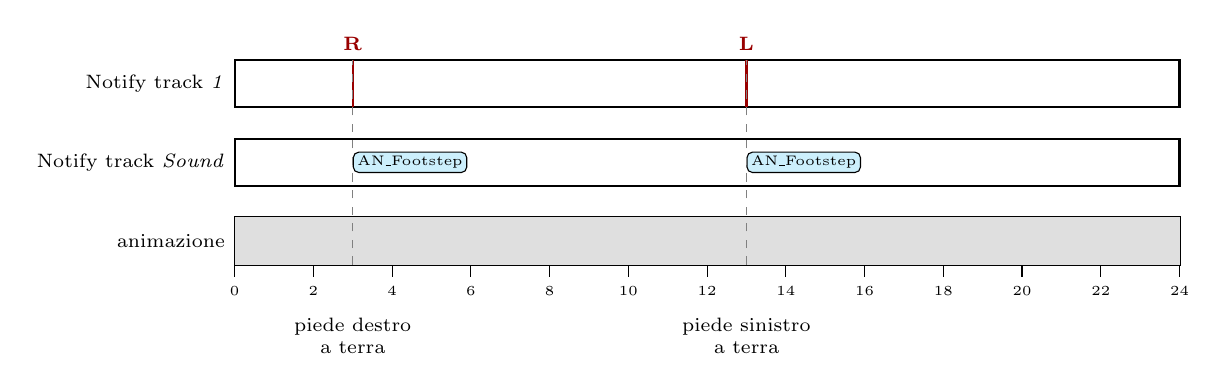
\begin{tikzpicture}[font=\footnotesize, x=0.5cm]
  \draw[thick] (0,0) rectangle (24,0.6);
  \node[left, font=\scriptsize] at (0,0.3) {Notify track \emph{1}};
  \draw[thick] (0,-1.0) rectangle (24,-0.4);
  \node[left, font=\scriptsize] at (0,-0.7) {Notify track \emph{Sound}};
  \draw[thick] (0,-2.0) rectangle (24,-1.4);
  \node[left, font=\scriptsize] at (0,-1.7) {animazione};
  \foreach \f in {0,2,...,24} {\draw (\f,-2.0) -- (\f,-2.15);
    \node[below, font=\tiny] at (\f,-2.15) {\f};}
  \fill[gray!25] (0,-2.0) rectangle (24,-1.4);
  \foreach \f/\n in {3/R, 13/L} {
    \draw[red!60!black, thick] (\f,0) -- (\f,0.6);
    \node[red!60!black, font=\scriptsize\bfseries, above] at (\f,0.6) {\n};
    \node[draw, fill=cyan!20, rounded corners=2pt, font=\tiny, inner sep=1.5pt, anchor=west]
      at (\f,-0.7) {AN\_Footstep};
    \draw[dashed, gray] (\f,-2.0) -- (\f,0.6);
  }
  \node[font=\scriptsize, align=center] at (3,-2.9) {piede destro\\a terra};
  \node[font=\scriptsize, align=center] at (13,-2.9) {piede sinistro\\a terra};
\end{tikzpicture}
\caption{La linea del tempo della corsa del bot (e delle due corse inclinate). Sulla
traccia \emph{1} i Sync Marker R e L ai frame 3 e 13; su una nuova traccia \emph{Sound}
l'AN\_Footstep negli stessi due punti. La lunghezza della linea del tempo è indicativa:
il numero totale di frame dell'animazione non si sente nella trascrizione. Schema
ricostruito.}
\label{ue10:fig:track}
\end{figure}

\paragraph{Approfondimento: Sync Marker, Blend Space e Notify doppi.} I Sync Marker non
sono legati alle ossa, come la trascrizione può far pensare, ma alla linea del tempo:
sono etichette con un nome (qui R e L) che segnano le fasi del passo. Servono quando
Unreal deve mescolare animazioni di durata diversa, nei Blend Space o con i
\emph{Sync Group}: invece di allinearle per tempo normalizzato, le allinea per marker, in
modo che i piedi tocchino terra insieme in tutte le animazioni mescolate. Funziona solo se
tutte le animazioni hanno gli stessi marker, con gli stessi nomi: è il motivo pratico per
cui il docente li aggiunge a tutte e tre le corse. I Notify, invece, pongono una domanda
diversa: in un Blend Space che sta mescolando tre animazioni, \emph{di quale} animazione
devono scattare i Notify? Nei Details del Blend Space, nella sezione \emph{Animation
Notifies}, l'opzione \emph{Notify Trigger Mode} decide: \emph{All Animations} (tutte quelle
che hanno un peso, con il rischio di sentire due o tre passi sovrapposti),
\emph{Highest Weighted Animation} (solo quella che pesa di più, la scelta più sicura per i
passi) o \emph{None}. Da notare infine che, nella lezione, la camminata a 250 non riceve
il Notify: a velocità intermedie i passi si sentono solo se il campione dominante è una
delle corse; per un risultato completo va aggiunto anche alla camminata, ai suoi frame di
appoggio. L'editor delle animazioni offre anche un Notify già pronto,
\emph{Play Sound}, che suona un suono senza Blueprint (il suo limite è che non sa
distinguere le superfici), e i \emph{Notify State}, che hanno un inizio e una fine invece
di un istante.

% ---------------------------------------------------------------------
\section{I Physical Material e le pedane}
\label{ue10:sec:physmat}

``Adesso, se noi andiamo in play, andiamo a vedere. Guardate un po'.'' A ogni passo
compare il trace che identifica il terreno, ``in questo caso il terreno di default''. ``Ma
come facciamo a dire, guarda, questo è un terreno diverso da quello normale? Dobbiamo
usare i Physics Material.''

\paragraph{Creare i Physical Material.} Una cartella \textbf{PhysicsMaterial} (``eccola
qua''); dentro, tasto destro, \textbf{Physics} $\rightarrow$ \textbf{Physical Material}. Se
ne creano due: \textbf{PM\_Rock} e \textbf{PM\_Water}. Poi, ``una cosa molto semplice,
ragazzi'': doppio clic su ciascuno; c'è la proprietà \textbf{Surface Type}, che di default
vale \emph{Default}: per PM\_Water si sceglie \textbf{Water}, per PM\_Rock \textbf{Rock}.
I nomi sono quelli scritti nelle Project Settings (figura~\ref{ue10:fig:catena}).

\paragraph{Le pedane.} ``L'unica cosa che ci manca è prendere una qualsiasi superficie.'' Un
blocco del livello, clonato (\textbf{Alt} più trascinamento, o duplicato) e schiacciato:
``fate un pianerottolino piccoletto'', due pedane. ``Adesso non abbiamo i materiali, ad
esempio, dell'acqua e della terra, ma ne mettiamo due a caso'': un materiale \emph{solid
blu} per l'acqua, \emph{Boulder} per la roccia; sono solo un segnale visivo. Poi:
selezionata la Static Mesh, ``andiamo giù, giù, giù, fino a trovare il \textbf{Phys
Material Override}'', e lì \textbf{PM\_Water} per l'acqua, \textbf{PM\_Rock} per la
roccia. ``Adesso, se noi andiamo sopra con il character, sentiamo che'' sulla roccia il
passo cambia. ``Eccolo qua.''

\begin{figure}[htbp]
\centering
\begin{tikzpicture}[font=\footnotesize,
  ue10box/.style={draw, thick, rounded corners=4pt, align=center, fill=gray!8,
                 minimum height=1.1cm, text width=2.5cm},
  ue10arr/.style={-{Stealth[length=2.5mm]}, thick}]
  \node[ue10box, fill=blue!8] (ps) at (0,0) {\textbf{Project Settings}\\{\scriptsize
    Engine, Physics, Physical Surface: Rock, Water}};
  \node[ue10box, fill=orange!12] (pm) at (4.3,0) {\textbf{PM\_Rock}, \textbf{PM\_Water}\\
    {\scriptsize Physical Material, Surface Type}};
  \node[ue10box, fill=green!10] (sm) at (8.6,0) {\textbf{Pedana}\\{\scriptsize Static
    Mesh, Phys Material Override}};
  \node[ue10box, fill=yellow!15] (tr) at (12.9,0) {\textbf{AN\_Footstep}\\{\scriptsize
    trace, Hit Result, Get Surface Type, Switch}};
  \node[ue10box, fill=violet!12] (cue) at (12.9,-2.4) {\textbf{Sound Cue}\\{\scriptsize
    Footstep, Rock, Water}};
  \node[ue10box, fill=red!10] (an) at (8.6,-2.4) {\textbf{Animazioni di corsa}\\
    {\scriptsize Notify ai frame 3 e 13}};
  \draw[ue10arr] (ps) -- node[above, font=\scriptsize]{nomi} (pm);
  \draw[ue10arr] (pm) -- node[above, font=\scriptsize]{assegnato} (sm);
  \draw[ue10arr] (sm) -- node[above, font=\scriptsize]{colpita} (tr);
  \draw[ue10arr] (tr) -- node[right, font=\scriptsize]{sceglie} (cue);
  \draw[ue10arr] (an.north east) -- node[below right, font=\scriptsize, pos=0.4]{fa
    scattare} (tr.south west);
\end{tikzpicture}
\caption{La catena completa dei passi. I nomi delle superfici nascono nelle Project
Settings, vengono assegnati ai Physical Material, che a loro volta si assegnano alle
superfici del livello; a ogni passo, il Notify inserito nell'animazione lancia il trace,
legge la superficie colpita e sceglie il Sound Cue. Schema ricostruito.}
\label{ue10:fig:catena}
\end{figure}

\paragraph{La spiegazione ripetuta.} A uno studente che chiede dove trovare ``i cosini''
(i PM): ``quelli li crei, praticamente. Lo fai con tasto destro, Physics, Physical
Material, e lo crei. Lo chiami PM\_Rock, come vuoi, PM\_Rock e PM\_Water. Ci clicchi su
ognuno di essi e gli cambi il Surface Type: lo metti Rock per il rock e Water per il
water. Poi, fatto questo, prendi un qualsiasi asset (vabbè, anche un blocco va
benissimo): devi andare su Phys Material Override e gli metti il Physical Material.''
``Basta che fai due pedanine'': ``qualsiasi superficie che tu vuoi prendere, ci puoi
camminare sopra''; ``la scali, fai quello che vuoi, fondamentalmente''.

\paragraph{Approfondimento: dove si assegna un Physical Material.} Il \emph{Phys Material
Override} usato a lezione vale per tutto il componente: comodo per una pedana, poco
pratico per un terreno che cambia da un punto all'altro. Unreal offre altri due posti. Il
primo è il \textbf{materiale}: nei Details di un Material (o di un Material Instance) c'è
la proprietà \emph{Phys Material}; tutte le mesh che usano quel materiale ``diventano''
roccia o acqua, senza toccare il livello, ed è la soluzione abituale nei progetti veri.
Il secondo è il \textbf{Landscape}: ogni layer dipinto può avere il suo Physical Material,
e il trace legge quello del layer dominante nel punto colpito. In più, il Physical
Material non serve solo ai suoni: contiene l'attrito (\emph{Friction}), il rimbalzo
(\emph{Restitution}) e la densità usati dalla simulazione fisica, ed è la base per gli
effetti d'impatto dei proiettili (scintille sul metallo, polvere sulla pietra), con la
stessa tecnica del Get Surface Type e dello Switch.

% ---------------------------------------------------------------------
\section{Gli ultimi problemi e la chiusura}
\label{ue10:sec:chiusura}

\paragraph{Gli ultimi problemi.} ``Un attimo: è successo un casino? Gli altri? Qualche
problema? Funziona?''
\begin{itemize}
  \item Uno studente si è perso il primo pezzo del grafo dell'AN\_Footstep e non sa da
        dove vengano Mesh Comp, Animation ed Event Reference: sono gli ingressi di
        Received\_Notify, la funzione sovrascritta con \emph{Override}. Poi, di nuovo, la
        catena: ``Get Owner, Get Actor Location, Get Actor Up Vector, e poi sottrai,
        per far sì che'' End sia sotto lo Start, ``che è il Get Actor Location''.
  \item Lo stesso studente ha messo le pedane, ma il personaggio non fa nessun rumore,
        nemmeno sul pavimento normale. I suoni nell'Anim Notify ci sono (``Rock1, Water
        Cue, Footstep Cue: va benissimo''); l'errore è nel vettore: il Get Actor Up Vector
        era collegato al pin sbagliato del Multiply. ``Mettilo sopra; stacca quello
        sotto; tasto destro su quello là, to float, 250.'' Con il Draw Debug Type a For
        Duration e una ricompilazione, il passo si sente.
  \item Le pedane, però, non fanno il suono della roccia: ``fammi vedere se hai messo la
        cosa'', e infatti il Phys Material Override non c'era. Lo studente non riesce a
        scendere nei Details fino alla voce: il pannello era filtrato su una categoria
        (\emph{Generale}); cliccando su \emph{Tutto} e aprendo la parte avanzata della
        sezione \emph{Physics} (``vai su tutto, clicca su tutto; giù, eccolo là''), si
        trova \emph{Phys Material Override}. ``A posto, perfetto.''
  \item ``A me non compaiono le linee'': ``basta che fai Draw Debug Type e la metti For
        Duration'', sul Line Trace By Channel. ``Quello è solo una cosa di debug,
        tranquilli.''
\end{itemize}

\paragraph{L'inclinazione rimandata.} ``Io ho sempre quella cosa dell'inclinazione della
testa'': è la studentessa del Lean che non inclina. ``Possiamo farlo la prossima volta?''
``Sì, facciamo la prossima volta. Tanto la prossima volta facciamo interazioni, e allora
ricordamelo tu, eh?'' ``Così fixiamo tutto''; ``lo guardo poi in futuro, lo guardo poi in
post anche''.

\paragraph{Il calendario.} ``Io vi ringrazio per l'attenzione, grazie'' anche a chi segue
in differita. ``Ci vediamo giovedì per la prossima lezione, che faremo in questo caso i
menu: andiamo a fare un po' di UI.'' (Il docente, poco prima, aveva parlato di
``interazioni'': dalla trascrizione non si capisce se la lezione di giovedì conterrà
entrambe le cose.) Uno studente pensava che oggi fosse giovedì; il calendario: ``abbiamo
questo martedì, giovedì e, se non sbaglio, il 30, che è martedì prossimo: è l'ultima con
me. Poi ci avete Davide.'' ``Va bene, ragazzi. Allora ci vediamo. Buona cena. Buona
serata.''

\begin{table}[htbp]
\centering
\small
\begin{tabular}{@{}p{5.4cm}p{8.6cm}@{}}
\toprule
\textbf{Sintomo} & \textbf{Causa e rimedio} \\
\midrule
Il personaggio non si muove, errori su IA\_Run & IA\_Move cancellata e sostituita da
IA\_Run: duplicare IA\_Look (Vector 2D), rinominarla IA\_Move, rimetterla in IMC\_Default
e nell'evento \\
L'evento del movimento non mostra il vettore & salvare l'Input Action; poi Split Struct
Pin sull'Action Value \\
Dopo una compilazione ``sparisce tutto'' & il Blueprint non compila: leggere i Compiler
Results \\
Camera storta, movimento strano & Spring Arm attaccato alla freccia o spostato dal pivot:
riattaccarlo, location a zero, usare Target Arm Length, Socket Offset, Target Offset \\
La camera non segue il mouse & Use Pawn Control Rotation sullo Spring Arm \\
La torretta ignora il nuovo personaggio & manca il tag Player; controllare le risposte
ai trace e alle collisioni \\
Il Montage non si vede & manca lo Slot DefaultSlot nell'AnimGraph \\
Durante il Montage il corpo gira & il DefaultSlot prende tutte le ossa: serve uno slot
per la parte alta (Layered blend per bone) \\
Errori nell'Event Graph incollato & variabili del vecchio ABP: ricrearle con Create
variable, rifare le referenze nell'Initialize \\
\emph{Idle to Walk will never be taken} & la regola della transizione non è ancora
scritta \\
Lo stato non mostra l'anteprima del Blend Space & lo stato non è mai raggiunto
(transizione o dati mancanti) \\
Il personaggio levita & Mesh a Z = $-90$ \\
Il personaggio si muove in T-pose & State Machine non collegata all'Output Pose, o
Mesh senza Anim Class \\
Errori su Jump e Fall & regole vuote: Automatic Rule Based on Sequence Player in State, e
la regola Fall $\rightarrow$ Land Run \\
GroundSpeed sempre zero & due variabili Character Movement (una mai valorizzata), o
Update non collegato al Validated Get \\
Il Lean non inclina & segno e scala del Delta Rotator, opzioni di rotazione; rimandato
alla lezione successiva \\
La camera inclinata di lato & ruotata sulla X (Roll) invece che sulla Y (Pitch) \\
AN\_Footstep non compare in Add Notify & la classe ha un altro nome: cercarla con quello
\\
Nessun suono di passi & Up Vector sul pin sbagliato del Multiply; Notify non inserito
nelle animazioni \\
Le pedane suonano come il pavimento & manca il Phys Material Override, o il Surface Type
del Physical Material \\
Phys Material Override introvabile & filtro dei Details su Generale: scegliere Tutto e
aprire le opzioni avanzate \\
Le linee del trace non si vedono & Draw Debug Type a For Duration \\
\bottomrule
\end{tabular}
\caption{I problemi incontrati durante la lezione, con la causa e il rimedio.}
\label{ue10:tab:errori}
\end{table}

\begin{table}[htbp]
\centering
\small
\begin{tabular}{@{}p{4.8cm}p{9.2cm}@{}}
\toprule
\textbf{Nodo, asset o impostazione} & \textbf{Che cosa fa} \\
\midrule
Input Action, Value Type Vector 2D & azione con un valore a due assi (movimento,
sguardo) \\
Add Movement Input & muove il Pawn lungo una direzione, con una scala \\
Tags (Actor) & etichette con cui altri Blueprint riconoscono l'actor \\
Try Get Pawn Owner / Cast To & il Pawn che possiede l'animazione; la sua classe precisa \\
Promote to Variable & salva un'uscita in una nuova variabile \\
Convert to Validated Get & Get con controllo di validità (Is Valid / Is Not Valid) \\
Create variable (tasto destro) & crea la variabile mancante di un nodo incollato \\
Comment (tasto C) / Reroute Node (doppio clic sul filo) & riquadro con titolo; punto di
piegatura di un filo \\
Blend Space 2D: Lean e GroundSpeed & mescola le corse inclinate e la camminata \\
Get Owning Actor / Get Actor Rotation & l'actor proprietario; la sua rotazione \\
Delta Rotator & la differenza normalizzata fra due rotazioni \\
FInterp To / RInterp To & un passo d'interpolazione fra float; fra rotator \\
Get World Delta Seconds & il tempo dell'ultimo frame \\
State Machine, Can Enter Transition & stati e regole booleane di passaggio \\
Automatic Rule Based on Sequence Player in State & la transizione scatta a fine
animazione \\
AND Boolean / NOT Boolean & congiunzione; negazione \\
Get Last Input Vector & l'ultimo input di movimento del Pawn (lunghezza 0--1) \\
Vector Length & la lunghezza di un vettore \\
Print String & scrive un valore a schermo, per il debug \\
World Settings: Default Pawn Class & il personaggio del giocatore nel livello \\
Anim Notify (classe), Received\_Notify & evento in un istante dell'animazione; la funzione
che lo riceve \\
Get Owner / Get Actor Location / Get Actor Up Vector & proprietario; posizione; vettore
verso l'alto \\
Line Trace By Channel, Draw Debug Type & trace lungo un segmento; disegno di debug \\
Break Hit Result: Impact Point & il punto esatto dell'impatto \\
Get Surface Type & il tipo di superficie colpita (dal Physical Material) \\
Physical Surface (Project Settings) & i nomi dei tipi di superficie \\
Switch on EPhysicalSurface & un'uscita per ogni tipo di superficie \\
Play Sound at Location & suona un suono in un punto \\
Sound Wave / Sound Cue & file audio; grafo che combina e modula i suoni \\
Create Single Cue & crea un Cue dai Sound Wave selezionati (con Random) \\
Random / Modulator & sceglie un ingresso a caso; varia pitch e volume \\
Add Sync Marker & marcatore con nome sulla linea del tempo (R, L) \\
Insert Notify Track / Add Notify & nuova traccia di Notify; inserisce un Notify \\
Physical Material: Surface Type & il tipo di superficie dell'asset \\
Phys Material Override & assegna un Physical Material a un componente \\
\bottomrule
\end{tabular}
\caption{I nodi, gli asset e le impostazioni della decima lezione.}
\label{ue10:tab:nodi}
\end{table}

% ---------------------------------------------------------------------
\section*{Punti chiave del capitolo}
\addcontentsline{toc}{section}{Punti chiave del capitolo}

\begin{itemize}
  \item Un'\textbf{Input Action} cancellata rompe il personaggio in modo silenzioso: si
        ricrea duplicando un'azione dello stesso tipo (\textbf{IA\_Look}, Vector 2D, per
        \textbf{IA\_Move}), la si rimette nell'\textbf{IMC} e nell'evento. Lo
        \textbf{Spring Arm} non si sposta dal pivot: si regolano Target Arm Length,
        Socket Offset e Target Offset.
  \item Quando si cambia personaggio, tutto ciò che riconosceva il vecchio va
        ricontrollato: \textbf{tag} (Player per la torretta), \textbf{cast} a classi
        precise, \textbf{collisioni} e risposte ai trace.
  \item Un Animation Blueprint si può costruire \textbf{copiando} l'Update di un altro, ma
        l'\textbf{Initialize} si rifà: Try Get Pawn Owner, Cast To, referenze promosse a
        variabile, ``un gancio'' fra animazione e personaggio. Le variabili mancanti si
        ricreano con \textbf{Create variable}; il \textbf{Validated Get} protegge l'Update.
        Attenzione alle variabili doppie (Character Movement 0).
  \item Ordine nel grafo: \textbf{commenti} con il tasto C, \textbf{Reroute} con un doppio
        clic sul filo.
  \item Il \textbf{Blend Space 2D} del bot ha il \textbf{Lean} in orizzontale ($-10$,
        10) e la \textbf{GroundSpeed} in verticale (0--500, la Max Walk Speed): corsa e
        corse inclinate a 500, camminata a 250, nessun Idle.
  \item Il \textbf{Lean} si calcola a ogni frame: rotazione attuale, \textbf{Delta
        Rotator} con quella precedente, lo \textbf{Yaw}, \textbf{FInterp To} verso quel
        valore (Interp Speed 1--5, Get World Delta Seconds), poi la rotazione attuale
        diventa la precedente. Segno e scala vanno verificati.
  \item La \textbf{State Machine} ha sette stati: Idle e Walk (GroundSpeed $>$ 0, $\le$
        0), Jump Idle e Jump Run (IsFalling AND la velocità), Fall (automatica dopo i
        salti), Land Idle e Land Run (NOT IsFalling AND [NOT] \textbf{ReceiveInput}),
        ritorni automatici. ReceiveInput viene da \textbf{Get Last Input Vector}: la
        lunghezza maggiore di zero dice che il giocatore sta premendo.
  \item Per giocare con il bot: Spring Arm e Camera a zero, Target Offset, \textbf{Default
        Pawn Class} nelle World Settings, i grafi di input copiati dal vecchio
        personaggio, Use Pawn Control Rotation, Mesh a $-90$.
  \item I passi: un \textbf{Anim Notify} (AN\_Footstep, \textbf{Received\_Notify}) lancia
        un \textbf{Line Trace By Channel} di 250 centimetri verso il basso; dal Hit Result,
        \textbf{Get Surface Type} e \textbf{Switch on EPhysicalSurface} scelgono il
        \textbf{Play Sound at Location} sull'\textbf{Impact Point}.
  \item I tipi di superficie si definiscono nelle \textbf{Project Settings} (Physics,
        Physical Surface: Rock, Water); i \textbf{Physical Material} (PM\_Rock, PM\_Water)
        li assegnano con il Surface Type; il \textbf{Phys Material Override} li applica
        alle mesh del livello.
  \item I \textbf{Sound Cue} variano i passi: \textbf{Random} fra più Sound Wave
        (\emph{Create Single Cue}) e \textbf{Modulator} sul pitch (passo 0,95--1,3, roccia
        2--2,2, acqua 1,3--1,5).
  \item Nelle animazioni di corsa: \textbf{Sync Marker} R e L e una \textbf{Notify Track}
        \emph{Sound} con l'AN\_Footstep ai frame di appoggio (3 e 13), in tutte e tre le
        animazioni.
\end{itemize}

%
%  Tutte le etichette di questo capitolo hanno il prefisso "ue10:"
%  (ue10:cap:..., ue10:sec:..., ue10:fig:..., ue10:tab:...), e tutti gli
%  stili TikZ hanno il prefisso "ue10" (ue10node, ue10exec, ue10data,
%  ...) per non collidere con chiavi native di TikZ né con quelli delle
%  lezioni precedenti. Il capitolo è autonomo: non contiene \ref verso
%  altri capitoli (i rimandi alle lezioni precedenti sono a parole).
%  Le figure sono ricostruzioni schematiche di quanto mostrato e detto a
%  lezione, non copie delle schermate del docente. Dove la trascrizione
%  è troppo rovinata per ricostruire un dettaglio, il capitolo lo dice
%  invece di inventarlo.
% =====================================================================

\chapter[Lean, State Machine e Physical Material]{Il nuovo personaggio: Lean,
State Machine e passi con i Physical Material}
\label{ue10:cap:bot}

Questa è la \textbf{decima lezione} del corso breve di \textbf{introduzione a Unreal
Engine}. Alla fine della nona il docente aveva lasciato un compito facoltativo: costruire
da zero un personaggio nuovo con lo \textbf{StackOBot}, il robottino dei progetti di
esempio di Epic, che ha già tutte le sue animazioni. Il compito era ``molto facoltativo,
perché capisco che è complicato''; in questa lezione lo si fa insieme, dall'inizio alla
fine: ``faremo proprio un nuovo character, che useremo poi come default''.

Il nuovo personaggio riprende la struttura del cavaliere della lezione precedente
(Animation Blueprint, State Machine, Blend Space), ma con tre differenze che danno il
titolo al capitolo. La prima è il \textbf{Lean}: il bot non ha otto animazioni
direzionali, ma una corsa e due varianti \emph{inclinate}, verso sinistra e verso
destra; il Blend Space 2D non usa più la direzione, ma un valore d'inclinazione calcolato
a ogni frame dalla differenza fra la rotazione attuale e quella del frame precedente. La
seconda è una \textbf{State Machine} più ricca, a sette stati, che distingue il salto da
fermo dal salto in corsa e l'atterraggio da fermo dall'atterraggio in movimento, con una
nuova variabile che dice se il giocatore sta premendo un tasto di movimento. La terza è
il suono dei \textbf{passi}: un \textbf{Anim Notify} inserito nelle animazioni, nel
momento esatto in cui il piede tocca terra, lancia un \emph{line trace} verso il basso,
legge il tipo di superficie colpita e suona il passo giusto; le superfici si distinguono
con i \textbf{Physical Material}, ``i materiali che possono determinare uno stato fisico''
di un oggetto. Sulla roccia si sente la roccia, sull'acqua l'acqua, altrove il passo
normale.

La lezione è \textbf{online}, su Zoom, come le precedenti. Si apre con una lunga
correzione in diretta del progetto di uno studente, prosegue con la costruzione del bot,
interrotta più volte dalle domande e dai problemi dei presenti, risolti in condivisione di
schermo, e si chiude sui passi e i Physical Material. La pausa arriva dopo la variabile
dell'input (``ci vediamo alle solite 18. Scusate: 17.55''); alla fine, ``vi mando a
cena''. È una lezione di \emph{fine corso}: ``mancano tre lezioni alla fine'', e il
docente lo ricorda per invitare chi segue in differita a entrare in diretta, se vuole
correzioni dal vivo.

Tre avvertenze di lettura, le stesse delle lezioni precedenti. La prima: la trascrizione
è automatica e storpia moltissimi nomi. Unreal è ``Arreal'', ``ArRIAL'', ``a Real'' e
``Arriva''; il \textbf{Lean} è ``Lin'', ``Line'', ``l'in'', ``LIN'' e ``Linn'' (``l'in è il
piegamento della rotazione''); l'\textbf{Idle} è ``idol'' e ``Idol''; l'\textbf{Event
Graph} è ``even graph'', ``Even Graph'' e ``Vengraph''; l'\textbf{AnimGraph} è
``Alimgraph'', ``aningraf'' e ``Aningraft''; \textbf{IA\_Move} è ``IAMove'', ``iam
move'', ``Iammov'' e ``gli ammove''; \textbf{IA\_Run} è ``iaran'', ``IRRun'' e ``iarran'';
l'\textbf{IMC} è ``IAMC'' e ``negli MC''; il \textbf{Then 0} della Sequence è
``DANZIRO'' e ``den zero''; i \textbf{Reroute Node} sono ``re Routenold''; il
\textbf{Blend Space} è ``Benzes'' e ``Brennese''; il \textbf{Validated Get} è ``validate
get''; l'\textbf{FInterp To} è ``F inter2'' e ``fintech 2''; l'\textbf{RInterp To} è ``R
inter to''; l'\textbf{Is Falling} è ``his falling'' e ``ease falling''; il \textbf{Last
Input Vector} è ``Lasting Pwn Vector''; lo \textbf{Spring Arm} è ``Springarma'' e
``spring guard''; \textbf{Use Pawn Control Rotation} è ``PoundCtrlRotation'', ``Pwn
rotation'' e ``use spawn control rotation''; le \textbf{World Settings} sono ``Word
Settings'' e la \textbf{Default Pawn Class} è ``default on class''; l'\textbf{Anim
Notify} è ``an in notify'', ``Anim Notifaj'', ``modify'', ``anni nota'' e ``anni
notifà''; \textbf{AN\_Footstep} è ``a n footstep'' e ``AN full step''; il
\textbf{Physical Material} è ``fisic material'' e ``P FIS materia''; \textbf{Get Surface
Type} è ``Gethsurfest Type'' e ``get sur festival''; il \textbf{Sound Cue} è ``queue'' e
``Q''; il \textbf{Draw Debug Type} è ``drop the bug type'' e ``draw the bug type''; il
\textbf{Break Hit Result} è ``break it risult''; \textbf{BP\_Knight} è ``BP Night'' e
``Night''; il \textbf{bot} è a tratti ``Boto'' e ``voto''. Dove la ricostruzione è
sicura il capitolo usa la forma corretta; dove non lo è riporta la forma della
trascrizione e lo dice. La seconda: all'inizio della registrazione e durante la pausa il
riconoscimento vocale produce lunghi blocchi di testo senza senso e ripetuto (``grazie a
tutti per l'attenzione che ci ha spiegato'', ``qual è la risposta che ci può essere?'',
``la situazione è questa, la migliore dal 2005'', il ``rinforzare la democrazia'', la
``dottrina sul mercato del lavoro'', il ``dialogo interculturale''): non appartengono
alla lezione e sono stati ignorati. La terza: buona parte della lezione è fatta di
indicazioni a voce mentre si lavora (``vai su'', ``clicca qua'', ``attacca quello
sotto''), spesso rivolte allo schermo di uno studente; il capitolo ricostruisce i grafi
da ciò che il docente dice mentre li costruisce, distingue i tentativi dalle soluzioni,
completa i nomi esatti dei nodi e dei pin di Unreal Engine 5, e dichiara i punti in cui
la trascrizione lascia un buco.

\paragraph{Come leggere questo capitolo.} Il capitolo segue l'ordine della lezione. Le
figure ricostruiscono il movimento riparato con l'Enhanced Input, i due eventi
dell'Animation Blueprint del bot con il Validated Get, il calcolo del Lean, il Blend
Space 2D del bot, la State Machine a sette stati, il grafo dell'Anim Notify dei passi, la
catena che porta dalla superficie al suono, il Sound Cue con Random e Modulator, e la
linea del tempo dell'animazione di corsa con i Sync Marker e i Notify. Le tabelle
riassumono le transizioni della State Machine, i valori dei Sound Cue, gli errori
incontrati durante la lezione e i nodi della giornata. Qua e là, dei paragrafi di
\textbf{approfondimento} collegano la lezione ai libri di Marcos Romero e Brenden Sewell
(\emph{Blueprints Visual Scripting for Unreal Engine 5} e la seconda edizione dello
stesso testo, scritta per Unreal Engine 4), i testi di riferimento per questa parte del
libro, e a qualche nozione tecnica generale su Unreal Engine 5; sono segnalati come tali
e non fanno parte della lezione.

Il percorso del capitolo:
\begin{enumerate}
  \item l'\textbf{inizio della lezione}: il movimento e la camera riparati in diretta
        (sezione~\ref{ue10:sec:riparazione});
  \item gli \textbf{annunci} e le domande: i passi e i Physical Material, il compito
        facoltativo, il personaggio nuovo che non interagisce con il livello, la lezione
        di giovedì, il bot di Federico (sezioni \ref{ue10:sec:annunci}
        e~\ref{ue10:sec:federico});
  \item il \textbf{risultato finale}, mostrato in anteprima
        (sezione~\ref{ue10:sec:demo});
  \item il nuovo personaggio: \textbf{Animation Blueprint} e \textbf{Blueprint
        Character}, l'Event Graph copiato, l'\textbf{Initialize} e il \textbf{Validated
        Get}, commenti e Reroute (sezioni da~\ref{ue10:sec:abp}
        a~\ref{ue10:sec:commenti});
  \item il \textbf{Blend Space 2D} del bot e il calcolo del \textbf{Lean} (sezioni
        \ref{ue10:sec:blend} e~\ref{ue10:sec:lean});
  \item la \textbf{State Machine} a sette stati, la variabile dell'\textbf{input} e le
        regole di transizione, prima e dopo la pausa (sezioni da~\ref{ue10:sec:sm}
        a~\ref{ue10:sec:transizioni2});
  \item il bot \textbf{in gioco}, con la camera, e il debug dei progetti degli studenti
        (sezioni \ref{ue10:sec:ingioco} e~\ref{ue10:sec:debug});
  \item i \textbf{passi}: l'\textbf{Anim Notify}, il \emph{line trace}, i
        \textbf{Physical Surface}, i \textbf{Sound Cue}, i \textbf{Notify} nelle
        animazioni e i \textbf{Physical Material} (sezioni da~\ref{ue10:sec:notify}
        a~\ref{ue10:sec:physmat});
  \item gli ultimi problemi e la \textbf{chiusura}
        (sezione~\ref{ue10:sec:chiusura}).
\end{enumerate}

% ---------------------------------------------------------------------
\section{Prima della lezione: il movimento da riparare}
\label{ue10:sec:riparazione}

Dopo i minuti iniziali di rumore della trascrizione, i saluti (``buongiorno, buon
pomeriggio'') e una prima richiesta. Mentre gli altri ``stanno ancora entrando'', uno
studente racconta il suo problema: ha seguito la lezione precedente in differita (``ho
seguito la lezione da quando è stata salvata''), e all'inizio ``andava tutto, si
muoveva''; poi, a un certo punto, il personaggio non si muoveva più, e ``la camera,
anche se segnata, non c'è, ed è sparito tutto''. Il docente propone di risolverlo subito
(``tanto adesso stanno ancora entrando'') e la correzione si fa in condivisione di
schermo. È una sequenza lunga e caotica, ma istruttiva: mostra come si legge un errore di
compilazione e come si ricostruisce un pezzo di Enhanced Input perduto.

\paragraph{Leggere gli errori.} ``Già ti dico che comunque possiamo già vedere gli
errori là sotto'': il pannello dei risultati della compilazione (\emph{Compiler
Results}) in fondo all'editor del Blueprint elenca i nodi che non trovano più ciò a cui
si riferiscono. La prima diagnosi, a colpo d'occhio: ``sicuramente ti manca
l'\emph{Input Action}''. L'errore dice che l'evento di \textbf{IA\_Run} non esiste più
nel nodo, o che il contesto \textbf{IMC\_Default} non lo contiene: ``dice che
fondamentalmente non hai IA\_Run: l'hai cancellato per sbaglio oppure non l'hai mai
creato?''. In realtà IA\_Run c'è (``il Content Browser, fai IA\_Run, ed eccolo là''): il
problema è un altro.

\paragraph{IA\_Move cancellata.} Aprendo l'\textbf{IMC\_Default} (``scrivi IMC, invece di
IAMC''), il docente trova dei mapping che lo studente non ricorda di aver messo (``ma no,
non li ho messi io''): li si cancella tutti con il cestino, poi si torna indietro con
\textbf{Ctrl+Z} (``fai Ctrl+Z a tutti, va benissimo''). Guardando il mapping che dovrebbe
essere \textbf{IA\_Move} si capisce: ``hai cancellato IA\_Move, fondamentalmente'', e al
suo posto, nell'Event Graph, l'evento del movimento è stato sostituito da IA\_Run (``ah,
perché l'hai sostituito''). ``E devi stare attento a queste cose.''

\paragraph{Ricreare IA\_Move.} ``La cosa che devi fare adesso è praticamente ricreare
IA\_Move.'' Il primo istinto è duplicare IA\_Run; poi il docente si corregge: ``no, no,
no: fai un doppione di \textbf{IA\_Look}''. Il motivo è il tipo di valore: IA\_Run è un
booleano (\emph{Digital}), mentre il movimento, come lo sguardo, è un \textbf{Vector 2D}
(``è un Vector 2D''): duplicare IA\_Look dà un'azione già del tipo giusto. Il doppione si
rinomina \textbf{IA\_Move}. Poi, nell'IMC\_Default:
\begin{itemize}
  \item si rimette IA\_Move nel mapping che lo usava prima (``adesso segnali negli MC
        quello di prima, IA\_Move'');
  \item con il \textbf{più} in alto si crea un altro mapping, per \textbf{IA\_Run}: con la
        freccina sotto il nome si apre la scelta del tasto e, invece di cercarlo nella
        lista, ``basta che clicchi sulla tastiera: clicca Shift sulla tua tastiera''. Il
        campo del tasto, quando è in ascolto, registra il primo tasto premuto.
\end{itemize}
Una compilazione di prova: ``qualche cosa si è levato, benissimo''.

\paragraph{L'evento e gli Add Movement Input.} Restano gli errori nell'Event Graph del
personaggio (il cavaliere, ``Knight''): ``hai sostituito IA\_Move con IA\_Run: devi levare
questo e mettere IA\_Move''; con il tasto destro si ricrea l'evento \textbf{IA\_Move}.
Uno strano dettaglio (``strano che non ti fa vedere'') si risolve salvando l'azione: solo
dopo il salvataggio l'evento mostra l'\textbf{Action Value} come vettore 2D. Si ricostruisce
il grafo del movimento, quello copiato la volta precedente dal ThirdPersonCharacter:
\begin{enumerate}
  \item tasto destro sull'\textbf{Action Value} e \textbf{Split Struct Pin}, per avere i
        pin \textbf{X} e \textbf{Y} separati;
  \item la \textbf{X} si collega al primo \textbf{Add Movement Input}, la \textbf{Y}
        ``tutto dritto fino a Scale Value del successivo'';
  \item il secondo Add Movement Input era stato cancellato (``ah, non c'è''): lo si
        ricopia dal primo (``copia Add Movement Input'');
  \item nella \textbf{World Direction} si collega ``quel forward vector che c'è lì
        vicino, quello arancione'' (il vettore di direzione calcolato dalla rotazione
        del controller);
  \item infine il pin di esecuzione: dal \textbf{Triggered} di IA\_Move, ``attacchi
        tutto in sequenza''.
\end{enumerate}
``E abbiamo riparato il movimento'' (figura~\ref{ue10:fig:move}). Compilato, il
personaggio si muove.

\begin{figure}[htbp]
\centering
\begin{tikzpicture}[font=\footnotesize,
  ue10node/.style={draw, thick, rounded corners=4pt, align=center, fill=gray!8,
                  minimum height=0.9cm, text width=3.4cm},
  ue10ev/.style={ue10node, fill=red!12},
  ue10exec/.style={-{Stealth[length=2.5mm]}, very thick, black!80},
  ue10data/.style={-{Stealth[length=2mm]}, thick, blue!60!black}]
  \node[ue10ev, text width=2.6cm, minimum height=2.0cm] (ev) at (0,0)
    {\textbf{IA\_Move}\\{\scriptsize Enhanced Input Action}\\{\scriptsize Action Value
    (Vector 2D), split in X e Y}};
  \node[ue10node] (a1) at (5.0,0.9) {\textbf{Add Movement Input}\\
    {\scriptsize World Direction: vettore destro; Scale Value: X}};
  \node[ue10node] (a2) at (10.0,0.9) {\textbf{Add Movement Input}\\
    {\scriptsize World Direction: vettore avanti; Scale Value: Y}};
  \node[ue10node, fill=green!10, text width=4.2cm] (rot) at (7.5,-1.9) {Get Control
    Rotation (solo lo Yaw) $\rightarrow$ vettori \textbf{Forward} e \textbf{Right}};
  \draw[ue10exec] (ev.east |- a1) -- node[above, font=\scriptsize]{Triggered} (a1);
  \draw[ue10exec] (a1) -- (a2);
  \draw[ue10data] (rot.west) -| node[pos=0.75, left, font=\scriptsize]{Right}
    (a1.south);
  \draw[ue10data] (rot.east) -| node[pos=0.75, right, font=\scriptsize]{Forward}
    (a2.south);
  \draw[ue10data, dashed] (ev.south) |- node[pos=0.75, below, font=\scriptsize]{X
    $\rightarrow$ Scale Value del primo, Y $\rightarrow$ Scale Value del secondo}
    (rot.south west);
\end{tikzpicture}
\caption{Il movimento riparato. L'Action Value di IA\_Move, un Vector 2D, viene diviso in
X e Y: la X muove lungo il vettore destro, la Y lungo quello in avanti, entrambi ricavati
dalla rotazione del controller. Se IA\_Move viene cancellata o sostituita da un'azione
booleana (IA\_Run), l'Action Value non è più un vettore e il grafo si rompe. Schema
ricostruito dal grafo standard del ThirdPersonCharacter; l'ordine esatto delle due
direzioni a lezione non si sente.}
\label{ue10:fig:move}
\end{figure}

\paragraph{Perché ``sparisce tutto''.} Lo studente aveva notato che a volte il
personaggio compariva e a volte, dopo una compilazione, ``proprio scompariva tutto''.
``È normale'': quando la compilazione di un Blueprint fallisce, Unreal ``te lo fa capire
in modo molto più palese'': l'icona del pulsante \emph{Compile} diventa rossa, con un
simbolo d'errore (``un'iconcina''), e un Blueprint che non compila non si comporta come
dovrebbe in gioco.

\paragraph{La camera storta.} In Play il movimento funziona, ma ``è un po' strano'', e la
camera è ``molto storta''. Tre correzioni, nell'ordine:
\begin{enumerate}
  \item \textbf{Use Pawn Control Rotation}: selezionato lo \textbf{Spring Arm}, si cerca
        ``control rotation'' e si mette la spunta (``mettilo true, perfetto''): la
        telecamera segue il controller.
  \item \textbf{La gerarchia}: la camera era stata agganciata alla \emph{freccia}
        (l'\emph{Arrow Component} del Character): ``attenzione a fare queste cose''. Lo
        Spring Arm va staccato dalla freccia e attaccato al suo posto; la Camera ``deve
        rimanere'' figlia dello Spring Arm.
  \item \textbf{La posizione}: lo Spring Arm era stato spostato con il \emph{pivot}
        (``l'hai spostato sulla location''): ``devi mettere tutto a zero''. Accanto ai
        valori della Location, nei Details, c'è una freccina circolare tutta a destra che
        li riporta al default.
\end{enumerate}
La regola, ripetuta: lo Spring Arm e la Camera non si muovono dal pivot, ``perché se no
si rompe tutto''. Per spostare la camera si usano solo i valori dello Spring Arm:
\textbf{Target Arm Length}, \textbf{Socket Offset} e \textbf{Target Offset}. ``Se muovi
il pivot, ti cambia la location del braccio, quindi ti fa tutto un effetto strano anche
con la camera.'' Siccome lo studente voleva una visuale più alta: \textbf{Target Offset},
Z (``l'ultima a destra'') a \textbf{60}. ``E già la telecamera dovrebbe essersi fissata
più o meno'': ``abbastanza bene''.

\paragraph{Le animazioni del giorno prima.} Lo studente aveva fatto anche ``la roba delle
animazioni'' (``oddio, è un po' buggato''), ma senza poterla provare, perché il
personaggio era fermo. ``Tanto oggi la riprenderemo'': si rifarà un personaggio ``proprio
da capo''.

% ---------------------------------------------------------------------
\section{Gli annunci e le domande}
\label{ue10:sec:annunci}

\paragraph{La cartella Footstep Sounds.} ``Oggi andremo a vedere anche una cosettina
interessante.'' Il docente l'ha scritto su Discord: nella cartella del materiale
didattico, su Drive, c'è una cartella \textbf{Footstep Sounds}; va scaricata e
decompressa, ``lasciatela là'', servirà più tardi. Servirà per i \textbf{Physical
Material}, ``cioè praticamente i materiali che possono determinare uno stato fisico, ad
esempio di un oggetto'': ``se un oggetto è di metallo, come deve reagire in certi
ambiti''. Oggi li si usa per i passi: ``quando lui fa superficie acquosa si sentirà il
rumore dei passi dell'acqua, se no si sentirà il rumore dei passi della roccia, o si
sentirà il rumore dei passi normale: dipende dalla superficie in cui ci troviamo''.

\paragraph{Le correzioni in diretta.} ``Visto che tanto oggi andiamo diretti in
editor'': chi ha problemi con le lezioni passate e vuole ``delle correzioni un po' in
live, rispetto a che magari in post'', ha ancora ``questa lezione, la prossima e la
prossima ancora'': ``mancano tre lezioni alla fine''. L'invito vale anche per chi segue in
differita: ``entri, se vuole delle correzioni direttamente in live''.

\paragraph{Il compito sul bot.} Uno studente chiede se il bot andava fatto ``per oggi'',
``perché io non so neanche dove mettere le mani''. Il docente ripete che era un compito
``per i più coraggiosi'', ``molto facoltativo'', ``per chi magari gli piace smanettare'':
``tanto oggi lo faremo''. E, a scanso di equivoci: ``non vi metto un voto, state
tranquilli''.

\paragraph{Il personaggio nuovo che non interagisce.} Lo stesso studente ha due problemi
con il suo personaggio. Il primo: ``corre, ma non ha l'animazione della corsa''. ``La
prima probabilmente sarà un errore che andremo a vedere insieme.'' Il secondo è più
interessante: il personaggio nuovo ``non interagisce più con molte delle cose che
abbiamo fatto nelle lezioni passate''. Il bottone per chiamare l'ascensore funziona, ma
salire sull'ascensore no; l'ascensore ``quello col suono'' sì; la torretta no. Il
docente spiega il caso della torretta, ed è un principio generale: quando si cambia
personaggio, tutto ciò che nel livello riconosceva il vecchio personaggio va
ricontrollato.
\begin{itemize}
  \item \textbf{Il tag}: ``la torretta funziona tramite il tag, come gliel'abbiamo
        fatta''. Nelle lezioni precedenti la torretta cercava un actor con il tag
        \textbf{Player}: ``quindi, se cambiamo character, dobbiamo rimettergli il tag'',
        cioè aggiungere \emph{Player} ai \emph{Tags} del nuovo Blueprint. ``Guarda che
        questo è il player: segui lui.''
  \item \textbf{Le collisioni}: il nuovo personaggio deve rispondere ``ai trace che
        abbiamo fatto'' (la torretta \emph{vede} il giocatore con un trace) e alle
        collisioni ``che sono, ad esempio, la sfera'' (la sfera che fa scattare la
        torretta quando il giocatore entra nel suo raggio).
\end{itemize}
``Intanto lo faremo oggi'': ``faremo un nuovo character e andremo poi a risistemare un po'
tutto''.

\paragraph{La lezione di giovedì.} ``Piccola postilla'': i \textbf{menu}, che erano
rimasti ``un po' un buco aperto'', si faranno come lezione \textbf{opzionale}
\textbf{giovedì}; poi ci sarà ``un'ultima lezione finale con un'ultima cosa''. Ma ``se
volete proporre anche qualche argomento che vi interessa, fatelo un po' oggi'': se gli
studenti si mettono d'accordo, ``facciamo quello''; ``se no, andiamo con i menu
tranquillamente''.

\paragraph{Approfondimento: tag, collisioni e personaggi intercambiabili.} Il problema
dello studente è tipico di ogni progetto in cui il personaggio cambia. Le soluzioni
viste nelle lezioni precedenti riconoscono il giocatore in tre modi diversi, e ciascuno
si rompe in modo diverso: per \emph{tag} (\emph{Actor Has Tag}: basta aggiungere il tag
al nuovo Blueprint, nella sezione \emph{Actor} $\rightarrow$ \emph{Tags} dei Details);
per \emph{cast} a una classe precisa (un \emph{Cast To BP\_Knight} fallisce con qualunque
altro personaggio: è il motivo per cui conviene fare il cast alla classe più generale che
serve, \emph{Character} o \emph{Pawn}, o usare un'interfaccia); per \emph{collisione}
(il nuovo personaggio ha la sua capsula e i suoi \emph{Collision Presets}: se i canali o
gli Object Type non corrispondono a quelli che il trace o l'overlap si aspettano, non
succede niente). Un ascensore che porta su il vecchio personaggio ma non il nuovo è quasi
sempre un problema del secondo o del terzo tipo. Romero e Sewell (capitolo 14) ricordano
che ``actor e componenti devono definire come reagiscono a ogni canale di trace e a ogni
object type'': \emph{Ignore}, \emph{Overlap} o \emph{Block}.

% ---------------------------------------------------------------------
\section{Il bot di Federico}
\label{ue10:sec:federico}

``Ci sono altre domande, ragazzi? Altri problemi, cose che serve fixare?'' Federico il
bot l'ha già fatto, e si è anche ``anticipato sui tempi'', con un tasto per interagire
(``vedo che ti sei anche anticipato sui tempi, effettivamente, sull'interactable''). Il
problema: premendo \textbf{F} il personaggio si ferma, si disabilita l'input e dovrebbe
partire un \textbf{Animation Montage}, ma l'animazione non si vede: ``posso solo girarmi''.

\paragraph{Il DefaultSlot che manca.} La diagnosi è la stessa della lezione precedente.
Nell'AnimGraph dell'ABP del bot (``ABP? L'Animation Blueprint''): ``devi mettere il
\textbf{DefaultSlot}'', ``quel passaggio che serviva praticamente per mixare le due
animazioni''. Fra la State Machine e l'Output Pose va il nodo \textbf{Slot}
(\emph{DefaultSlot}): ``vai dentro, dentro, e poi fuori''. Compilato, l'animazione
parte: ``perfetto, ottimo''.

\paragraph{Il personaggio che gira su se stesso.} Durante l'animazione, però, il bot
``si gira''. Una prima correzione: nel Blueprint del bot, selezionato il componente in
cima alla lista (``schiaccia proprio sulle componenti, tutto a sinistra'', cioè il
Blueprint stesso o il suo Character Movement), si cerca ``rotation'' e si toglie
\textbf{Use Controller Desired Rotation} (``fai leva use control desired rotation''). Ma
il problema vero è un altro, e il docente lo rimanda: ``quello fondamentalmente lo
possiamo fare con l'\emph{upper slot}, che poi magari lo possiamo vedere''. ``È normale che
lui giri su se stesso, perché il DefaultSlot prende tutte le ossa del corpo'': il
Montage sostituisce la posa dell'intero scheletro, gambe comprese, mentre il personaggio
continua a muoversi e a ruotare con la camera (``io lo muovo col WASD''; ``però si muove
comunque con la telecamera''). ``Il fatto è che bisogna mixare le due animazioni'': la
parte alta del corpo dal Montage, quella bassa dalla locomozione. ``Poi adesso ti faccio
vedere magari come fare le animazioni.''

\paragraph{Approfondimento: l'upper slot e il Layered Blend per Bone.} Lo slot di cui
parla il docente è la tecnica standard per animare solo metà del corpo. Si crea un nuovo
slot (per esempio \emph{UpperBody}) nel \emph{Anim Slot Manager} dello scheletro, si
assegna il Montage a quello slot invece che al DefaultSlot, e nell'AnimGraph si usa un
nodo \textbf{Layered blend per bone}: la posa base (la locomozione) entra nel primo
ingresso, la posa con lo slot nel secondo, e nei Details del nodo si indica l'osso da
cui la seconda posa comincia a valere (di solito la colonna, \emph{spine\_01} o
equivalente), con un \emph{Blend Depth}. Il risultato è un personaggio che attacca o
interagisce con le braccia mentre le gambe continuano a camminare. Il resto del
fenomeno, il corpo che ruota con la camera, dipende dalle tre spunte di rotazione già
viste nella lezione precedente (Use Pawn Control Rotation, Use Controller Rotation Yaw,
Orient Rotation to Movement) e da \emph{Use Controller Desired Rotation}, che fa ruotare
il personaggio verso la rotazione del controller con la velocità indicata in
\emph{Rotation Rate}.

% ---------------------------------------------------------------------
\section{Il risultato finale, in anteprima}
\label{ue10:sec:demo}

``Allora, ragazzi, oggi andremo a fare questo bellissimo bot.'' Prima un controllo
sull'audio (``non sentite l'audio? Datemi un feedback''): bisogna condividere anche
l'audio del computer, in Zoom. Poi la dimostrazione: il bot del docente cammina sul
livello e, ``se voi fate attenzione, ci sta un piccolo trace sotto, che appare ai piedi
del nostro bot''. ``E praticamente va a identificare, a ogni passo, la tipologia di
materiale che lui sta toccando in questo momento.'' Sul pavimento normale si sente il
passo normale; sopra una pedana blu (``questa è l'acqua'') a ogni passo si sente l'acqua;
``allo stesso tempo anche la roccia''. ``Questi qua sono fatti con i Physics Material.''

\paragraph{Dove si trova il Physical Material.} ``Se voi cliccate su qualsiasi asset''
nel livello, per esempio una Static Mesh, e nella barra di ricerca dei Details scrivete
``phys'', trovate \textbf{Phys Material Override} (``lo accorcia: Phys Materia
Override''): lì il docente ha messo un asset che ha creato, \textbf{PM\_Rock}, ``Physic
Material Rock''. ``Possiamo differenziare le tipologie di superfici tramite una cosa di
Unreal che ci permette di dire: guarda, puoi creare tutta una varietà di superfici,
ognuna ha una sua regola, volendo, su come reagisce a tutto quanto.'' Il caso di oggi è
``la cosa più semplice'': ``guarda, questa è la roccia: quando stai sulla roccia fammi
questo suono; se invece stai sull'acqua, fammi quest'altro suono''.

``Come facciamo? Allora, intanto andiamo a fare il nostro character, innanzitutto.''

% ---------------------------------------------------------------------
\section{Il nuovo Animation Blueprint e il nuovo Character}
\label{ue10:sec:abp}

\paragraph{La cartella e l'ABP.} Nella cartella dei personaggi si crea una nuova
cartella per il bot (il docente aggiunge un ``2'' a tutti i nomi, perché il suo progetto
ha già un bot: ``glielo chiamerò 2''). Il primo asset è l'\textbf{Animation Blueprint}:
alla creazione Unreal chiede lo \textbf{scheletro}, e ``a noi ci interessa'' quello del
bot, lo scheletro della Skeletal Mesh del bot (\emph{SK\_Bot}, nella trascrizione
``character SH bot'' e ``scheda dal mesh del bot''), ``come abbiamo visto e come abbiamo
creato anche gli altri character''. Lo si chiama \textbf{ABP\_Bot2} e lo si apre.

\paragraph{Copiare l'Event Graph.} ``Anche senza fare troppe cose, perché tanto l'abbiamo
già fatte'': si apre \textbf{ABP\_Knight}, l'Animation Blueprint del cavaliere della
lezione precedente (o quello del proprio personaggio), e si va nel suo \textbf{Event
Graph}. La parte dell'\textbf{Update} ``può essere tranquillamente uguale. Perché cosa
fa? Questi sono semplicemente calcoli'': la GroundSpeed, se sta cadendo, la direzione.
Quindi la si seleziona, \textbf{Ctrl+C}, e la si incolla con \textbf{Ctrl+V} nell'Event
Graph di ABP\_Bot2. La parte dell'\textbf{Initialize}, invece, no: ``bisognerà sicuramente
fare la stessa cosa, ma non copiamo questo'', perché fa il cast a una classe precisa, il
cavaliere, e il bot ha bisogno di un Blueprint suo, che ancora non esiste. L'AnimGraph,
anche lui, ``lo rifaremo per forza, perché sarà totalmente diverso''.

\paragraph{BP\_Bot2.} Nella stessa cartella: \textbf{Blueprint Class}, \textbf{Character},
nome \textbf{BP\_Bot2}. Nel Blueprint, selezionato il componente \textbf{Mesh}:
\begin{itemize}
  \item \textbf{Skeletal Mesh Asset}: la Skeletal Mesh del bot;
  \item la mesh si trascina ``un po' più in basso'', fino ai piedi della capsula, e la si
        ruota di 90 gradi sulla Z, perché guardi nella direzione della freccia (la
        posizione esatta, \textbf{Z = $-90$}, la si fisserà più avanti, quando il
        personaggio ``levita'');
  \item \textbf{Anim Class}: \textbf{ABP\_Bot2}, ``in modo tale che lui poi prenda le
        animazioni, il ragionamento che andrà a fare''.
\end{itemize}
A uno studente che non trova dove si collega l'Animation Blueprint: ``se tu clicchi
sulla Mesh, devi collegargli l'Animation Blueprint'', nel campo \emph{Animation Class}
dei Details. ``Fatto. Grazie, perfetto.''

% ---------------------------------------------------------------------
\section{L'Initialize del bot e il Validated Get}
\label{ue10:sec:initialize}

\paragraph{Le variabili da rifare.} L'Event Graph incollato ``è normale'' che dia errori:
le sue variabili (le referenze al cavaliere e al suo Character Movement) appartengono a
un altro Blueprint. ``Dobbiamo semplicemente levare tutte queste variabili qua, perché le
dobbiamo rifare tutte. Però intanto ci abbiamo la struttura.''

\paragraph{Event Blueprint Initialize Animation.} Si rifà l'Initialize come la volta
precedente, ma per il bot:
\begin{enumerate}
  \item \textbf{Event Blueprint Initialize Animation};
  \item \textbf{Try Get Pawn Owner} e \textbf{Cast To BP\_Bot2} (``andando a fare un cast
        tra il Get Pawn Owner e il BP\_Bot'');
  \item dall'uscita del cast, \textbf{Promote to Variable}: la referenza al bot,
        \textbf{AsBP\_Bot2} (``promuoviamo a variabile la referenza'');
  \item dalla referenza, \textbf{Character Movement}, anche lui promosso a variabile.
\end{enumerate}
``Questa è una prassi, ragazzi'': ``prendere tutte le referenze, in modo tale che possano
comunicare'' l'Animation Blueprint e il Blueprint del personaggio.

\paragraph{Il Validated Get.} Nell'Update, prima di leggere i dati, la referenza al bot va
controllata. Invece del nodo \textbf{Is Valid}, ``a noi ci interessa farla tranquillamente
con questo \textbf{Validated Get}'': si trascina nel grafo un \emph{Get} della variabile
AsBP\_Bot2, tasto destro sul nodo e, in fondo al menu, \textbf{Convert to Validated Get}.
Il Get diventa un nodo con un ingresso di esecuzione e due uscite, \textbf{Is Valid} e
\textbf{Is Not Valid}: ``è un get che serve per dire: ehi, guarda, questa variabile
all'interno è valida, in automatico, senza fare il blocco Is Valid''. Lo si collega a
\textbf{Event Blueprint Update Animation}, e dall'uscita \emph{Is Valid} parte la
\textbf{Sequence} incollata. ``Perché, se questa referenza non c'è, ci sono errori'':
``esiste BP\_Bot? Se non esiste, non faccio niente'', ``se non esiste il BP che mi comanda
tutto''. Il caso tipico è la preview dell'editor dell'Animation Blueprint, dove la mesh non
appartiene a nessun personaggio e il cast fallisce.

\paragraph{Ricollegare e ricreare.} Poi si rimettono le referenze nei nodi incollati: per
la \textbf{Velocity} e per l'\textbf{Is Falling} il \textbf{Character Movement}, ``perché
sono tutte particolarità del movimento''; dove serve il personaggio, la referenza
\textbf{AsBP\_Bot2}. Le variabili di destinazione (Velocity, GroundSpeed, IsFalling) non
esistono ancora in ABP\_Bot2, e i loro nodi \emph{Set} sono segnati come errori: ``potete
tranquillamente ricrearle molto facilmente: cliccandoci sopra, tasto destro, e c'è
scritto proprio \textbf{Create variable}'' (per esempio, \emph{Create variable
Velocity}). ``Lo fate per tutte quante. Adesso compilate e siamo a posto''
(figura~\ref{ue10:fig:abpevents}).

``Questo, ragazzi, è come si copia e incolla una lezione'': ``per non rifare le stesse
cose che abbiamo fatto volte e volte e volte, continuamente''.

\begin{figure}[htbp]
\centering
\begin{tikzpicture}[font=\footnotesize,
  ue10node/.style={draw, thick, rounded corners=4pt, align=center, fill=gray!8,
                  minimum height=0.9cm, text width=2.3cm},
  ue10ev/.style={ue10node, fill=red!12},
  ue10var/.style={ue10node, fill=blue!10, rounded corners=8pt},
  ue10exec/.style={-{Stealth[length=2.5mm]}, very thick, black!80},
  ue10data/.style={-{Stealth[length=2mm]}, thick, blue!60!black}]
  % Initialize
  \node[ue10ev, text width=2.6cm] (ini) at (0,0) {\textbf{Event Blueprint Initialize
    Animation}};
  \node[ue10node] (pawn) at (0,-1.8) {\textbf{Try Get Pawn Owner}};
  \node[ue10node] (cast) at (3.9,0) {\textbf{Cast To BP\_Bot2}};
  \node[ue10var] (s1) at (7.4,0) {\textbf{Set} AsBP\_Bot2};
  \node[ue10var] (s2) at (10.9,0) {\textbf{Set} Character Movement};
  \node[ue10node, text width=2.0cm] (cm) at (9.15,-1.8) {Character Movement
    {\scriptsize (componente)}};
  \draw[ue10exec] (ini) -- (cast); \draw[ue10exec] (cast) -- (s1);
  \draw[ue10exec] (s1) -- (s2);
  \draw[ue10data] (pawn.east) -- ++(0.5,0) |- node[pos=0.25, right,
    font=\scriptsize]{Object} ([yshift=-3mm]cast.west);
  \draw[ue10data] ([yshift=-3mm]cast.east) -- ([yshift=-3mm]s1.west);
  \draw[ue10data] (s1.south) |- (cm.west);
  \draw[ue10data] (cm.east) -| (s2.south);
  % Update
  \node[ue10ev, text width=2.6cm] (upd) at (0,-4.0) {\textbf{Event Blueprint Update
    Animation}};
  \node[ue10node, fill=yellow!15, text width=2.4cm] (vg) at (3.9,-4.0)
    {\textbf{GET} AsBP\_Bot2\\{\scriptsize (Validated Get)}};
  \node[ue10node, text width=1.6cm] (seq) at (7.4,-4.0) {\textbf{Sequence}};
  \node[ue10node, text width=3.4cm, align=left] (t0) at (11.2,-3.0)
    {{\scriptsize Then 0:} Velocity, GroundSpeed};
  \node[ue10node, text width=3.4cm, align=left] (t1) at (11.2,-4.1)
    {{\scriptsize Then 1:} IsFalling};
  \node[ue10node, text width=3.4cm, align=left] (t2) at (11.2,-5.2)
    {{\scriptsize poi:} Lean, ReceiveInput};
  \node[font=\scriptsize, text width=2.4cm, align=center] at (3.9,-5.1)
    {Is Not Valid: nulla};
  \draw[ue10exec] (upd) -- (vg);
  \draw[ue10exec] (vg) -- node[above, font=\scriptsize]{Is Valid} (seq);
  \draw[ue10exec] (seq.east) -- ++(0.5,0) |- (t0.west);
  \draw[ue10exec] (seq.east) -- ++(0.5,0) |- (t1.west);
  \draw[ue10exec] (seq.east) -- ++(0.5,0) |- (t2.west);
\end{tikzpicture}
\caption{I due eventi di ABP\_Bot2. In alto, l'Initialize, una volta sola: dal Pawn
Owner al cast, alle due referenze salvate. In basso, l'Update, a ogni frame: il
Validated Get blocca tutto se la referenza al bot non è valida; poi la Sequence esegue i
calcoli. La Then 0 e la Then 1 vengono dall'Event Graph di ABP\_Knight; il calcolo della
direzione, che lì stava su un'altra uscita, viene eliminato e sostituito dal Lean;
l'ultima uscita si aggiunge prima della pausa. Schema ricostruito.}
\label{ue10:fig:abpevents}
\end{figure}

\paragraph{Che cosa fa l'Initialize: la spiegazione.} Più tardi, durante il lavoro sul
Lean, una studentessa chiede che cosa fosse ``il blocco di nodi tutto sopra'', quello
``che abbiamo dovuto fare a mano''. La risposta del docente è il riassunto più chiaro
della lezione su questo punto. ``Quando inizializzi le animazioni, in generale, cosa
andiamo a fare? Prova a prendere il Pawn Owner, nel senso il proprietario.'' Ogni
character ha un pawn: ``il pawn, ricordiamo, non è il character: è l'entità che controlla
il character''; il character ``è la mesh con le animazioni''. ``Quindi dice: vammi a
prendere il pawn che ha questa animazione, che ha questo character.'' Poi il cast:
``andiamo a cercare di comunicare direttamente con quel preciso actor, quindi BP\_Bot''.
E le referenze: ``visto che ci serviranno un sacco di cose'', i valori della velocità e
del ``sta cadendo'', che sono controllati dal Character Movement (``è lui che lavora sulla
velocity e comunque la controlla''; ``la possiamo prendere solamente se abbiamo un
Character Movement a portata di mano''), ``andiamo a dire: guarda che mi devi fare una
referenza a questa comunicazione''. ``Come dirti, è un \emph{gancio}: io mi lascio il
gancetto attaccato, così almeno io comunico con te.'' ``Crea una via di comunicazione tra
l'animazione, cioè l'Animation Blueprint, e in questo caso BP\_Bot'': ``come BP\_Bot2,
fammi queste azioni; oppure, come Character Movement di BP\_Bot2, fammi queste azioni''.

\paragraph{Approfondimento: il Validated Get e l'AnimGraph nel libro.} Romero e Sewell
(capitolo 16, nel modello VR) usano il Validated Get esattamente come la lezione:
``quando avete un nodo Get di una referenza a oggetto, potete cliccarci con il tasto
destro e scegliere \emph{Convert to Validated Get}''; il nodo diventa ``un nodo GET con dei
pin di esecuzione che si possono usare per controllare se la referenza è valida''. Nel
capitolo 4 gli stessi autori raccomandano di usare sempre l'Is Valid prima di eseguire una
funzione su una referenza: il Validated Get è la stessa cosa in un nodo solo. Il capitolo
17 spiega poi perché serve tutto questo lavoro di referenze nell'Event Graph: ``l'AnimGraph
può accedere solo alle variabili dell'Animation Blueprint, quindi usiamo l'Event Graph per
prendere i valori aggiornati dal Pawn''. Nel loro esempio il calcolo è il più semplice
possibile: \emph{Try Get Pawn Owner}, \emph{Get Velocity}, \emph{VectorLength}, e il
risultato nella variabile \emph{Speed}. Una nota tecnica: in Unreal Engine 5 l'Event Graph
dell'Animation Blueprint gira sul \emph{game thread}; per personaggi numerosi Epic consiglia
di spostare i calcoli nella \emph{Blueprint Thread Safe Update Animation} e di leggere i
dati con le \emph{Property Access}, ma per un personaggio solo la tecnica della lezione è
del tutto adeguata.

% ---------------------------------------------------------------------
\section{Ordine nel grafo: commenti e Reroute}
\label{ue10:sec:commenti}

\paragraph{I commenti.} Mentre gli studenti ricopiano, il docente ne approfitta per un po'
di pulizia: ``potete creare dei commenti premendo \textbf{C}''. Selezionati dei nodi,
il tasto C crea un riquadro intorno a loro, ``queste schedine che sono i commenti'', con
un titolo. Il docente commenta i blocchi dell'Update: \textbf{Check Actual Velocity},
\textbf{Check Is Falling}, \textbf{Check Direction} (``la sua direzione''). ``Così viene
un codice più ordinato per tutti quanti''; ``questo lo sto facendo io per pulizia,
ragazzi: se siete indietro, non mi seguite, tranquilli''.

\paragraph{Then 0.} Uno studente ha ``nodi diversi'' e chiede che cosa sia il
``DANZIRO'': è il \textbf{Then 0} della \textbf{Sequence}, la prima uscita, quella che nel
grafo copiato porta al calcolo della velocità: ``il Then 0 dice la velocity'';
``questo fondamentalmente è il calcolo della velocity''.

\paragraph{I Reroute Node.} ``Come fai a mettere quei puntini bianchi?'' Sono i
\textbf{Reroute Node}: si creano con un \textbf{doppio clic sul filo}, e si possono
trascinare per piegare il collegamento. ``Permettono di avere un po' più di ordine.''

\paragraph{Approfondimento: commenti, Reroute e scorciatoie nel libro.} Romero e Sewell
(capitolo 15, \emph{Blueprints Tips}) descrivono le stesse due tecniche: ``per creare un
riquadro di commento intorno ad alcuni nodi, selezionate i nodi, poi cliccate con il tasto
destro su uno di essi e scegliete \emph{Create Comment from Selection}, oppure premete
semplicemente il tasto C''; il commento ``aiuta a identificare un blocco di logica, e la
sua etichetta resta visibile'' anche quando si allontana lo zoom. Nel capitolo 11, durante
la costruzione di una macro, notano che ``si può fare doppio clic su un filo per
aggiungere un Reroute Node e modificare la forma e la posizione del filo''. Nello stesso
capitolo 15 ricordano altre scorciatoie da tastiera per i nodi più comuni (B più clic per
un Branch, S per una Sequence, D per un Delay, F per un For Each Loop), oltre al tasto Q
per allineare i nodi già visto nella lezione precedente.

% ---------------------------------------------------------------------
\section{Il Blend Space 2D del bot}
\label{ue10:sec:blend}

\paragraph{Creare il Blend Space.} Tasto destro, \textbf{Animation}, \textbf{Blend Space}:
\textbf{BS\_Bot2}. Uno studente non lo trova (``abbiamo perso il Blend Space''): tasto
destro, categoria Animation, Blend Space. Un altro chiede quale dei due: ``quello non
differenziato è quello 2D, cioè quello in cui non c'è scritto niente; quello 1D c'è
sempre scritto 1D''. Serve il \textbf{2D}.

\paragraph{Le animazioni di Lean.} Prima di riempirlo, il docente mostra che cosa ha il
bot: ``abbiamo delle animazioni che si chiamano \emph{lean}'' (le aveva già usate
Federico). ``Lean è lo spostamento verso sinistra, verso destra'': il bot ``sta comunque
camminando dritto, ma sta, come dire, spostato'', inclinato da una parte. ``Serve un po'
per dare questa cosa di movimento al character'': quando il personaggio curva, il corpo si
piega verso l'interno della curva, come un corridore.

\paragraph{I due assi.} ``Nel 2D ci sono due dati che vanno a capire come è il
movimento.'' Nei Details, \textbf{Axis Settings}, aprendo la freccina di ciascun asse si
trova il nome (``potete dare il nome da qua a sinistra''):
\begin{itemize}
  \item \textbf{Horizontal Axis}: \textbf{Lean}, minimo \textbf{$-10$}, massimo
        \textbf{10};
  \item \textbf{Vertical Axis}: ``la nostra bellissima, conosciutissima''
        \textbf{GroundSpeed}, da \textbf{0} alla velocità del personaggio.
\end{itemize}
La velocità massima del bot, nel Character Movement di BP\_Bot2, è la \textbf{Max Walk
Speed} di default, \textbf{600}. ``Ma facciamolo un po' più lento, dai, facciamolo più
lentino'': \textbf{500}. ``Tenetevi questi due aperti'': nel Blueprint, Character
Movement, Max Walk Speed a 500; nel Blend Space, \textbf{Maximum Axis Value} della
GroundSpeed a 500.

\paragraph{Una domanda: legare l'asse alla Max Walk Speed?} Uno studente ha un problema
che ha incontrato più volte: calibra il Blend Space sui passi (per esempio, la corsa a
300), poi decide che 300 è la velocità massima e la corsa non parte più; oppure, cambiata
la velocità, il personaggio fa ``l'animazione di corsa anche mentre cammina''. Ogni volta
deve ritoccare a mano il massimo dell'asse e la posizione delle animazioni: ``non c'è un
modo per farlo veloce?'', cioè per collegare la Max Walk Speed al Maximum Axis Value?
``Purtroppo questo no: non so se ci sta un metodo, almeno non lo so, ma spero di sì. Però
non l'ho mai visto. Effettivamente sarebbe molto comodo.'' E un avvertimento: ``se tu
cambi dei valori, specialmente se lo fai più piccoli, ti fa un casino'', e a volte
conviene levare tutte le animazioni e rifare il Blend Space da capo. ``Sicuramente mi
informerò, perché è una cosa che anch'io ambisco tantissimo, devo essere sincero.''
Allo studente, che aveva usato GroundSpeed e direzione per stabilire il lean, il docente
consiglia di invertire gli assi: ``sulla verticale metti la speed, sull'orizzontale metti
la lean'', e di seguire il procedimento della lezione.

\paragraph{I campioni.} Le animazioni si trascinano sulla griglia (con \textbf{Shift} si
agganciano ai punti precisi: ``potete praticamente anche snappare i keyframe, tenendo
premuto Shift''). La disposizione (figura~\ref{ue10:fig:blend}):
\begin{itemize}
  \item la \textbf{corsa} (\emph{Bot Run}) al centro in alto, Lean 0 e GroundSpeed 500:
        ``la mettiamo centrale, perché ricordiamo che stiamo dividendo'';
  \item il \textbf{Lean Left} a $-10$, sempre a 500 (``500, meno 10''), e il \textbf{Lean
        Right} a 10: ``negativo è sinistra, positivo è destra''. Più che un'animazione
        diversa, ``sarà praticamente la rotazione del nostro character che determinerà il
        fatto che lui si muova un po', si inclini a destra e a sinistra'';
  \item in mezzo, ``come animazione di appoggio'', la \textbf{camminata} (\emph{Bot
        Walk}) a Lean 0 e GroundSpeed \textbf{250}: ``andiamo a creare questo
        triangolino''.
\end{itemize}
Uno studente si è perso un valore: la GroundSpeed va da 0 a 500 (``minimum 0, maximum
500''); la walk ``è 250''. Il nome esatto degli asset di animazione dello StackOBot non si
ricostruisce dalla trascrizione; il capitolo usa nomi descrittivi.

\paragraph{E l'Idle?} ``Scusami, ma dove sta l'Idle? Non la metteremo, ragazzi.'' Il
motivo: il bot ha due atterraggi diversi, \emph{Land Idle} e \emph{Land Run}, ``nel senso
che lui atterra dopo un salto: se sta fermo, va e ritorna in Idle; oppure, se lui atterra
e però sta camminando'', continua a camminare. Per poter distinguere i due casi, la
differenza fra fermo e in movimento va fatta nella \textbf{State Machine}, con uno stato
\emph{Idle} separato, e non dentro il Blend Space (sezione~\ref{ue10:sec:sm}). È la scelta
opposta a quella della lezione precedente, dove il Blend Space del cavaliere conteneva anche
l'Idle a velocità zero.

\begin{figure}[htbp]
\centering
\begin{tikzpicture}[font=\footnotesize, x=0.45cm, y=0.011cm,
  ue10pt/.style={draw=black, fill=white, thick, diamond, inner sep=2.2pt}]
  \draw[step=1, gray!20] (-10,0) grid[xstep=2.5, ystep=62.5] (10,500);
  \draw[thick] (-10,0) rectangle (10,500);
  \draw[-{Stealth[length=2.5mm]}, thick] (-10,0) -- (11.2,0) node[right]{Lean};
  \draw[-{Stealth[length=2.5mm]}, thick] (-10,0) -- (-10,560) node[above]{GroundSpeed};
  \foreach \x in {-10,-5,0,5,10} \node[below, font=\scriptsize] at (\x,0) {\x};
  \foreach \y in {0,250,500} \node[left, font=\scriptsize] at (-10,\y) {\y};
  \node[ue10pt] (l) at (-10,500) {}; \node[ue10pt] (r) at (0,500) {};
  \node[ue10pt] (rr) at (10,500) {}; \node[ue10pt] (w) at (0,250) {};
  \node[above=3pt of l, font=\scriptsize\bfseries] {Lean Left};
  \node[above=3pt of r, font=\scriptsize\bfseries] {Run};
  \node[above=3pt of rr, font=\scriptsize\bfseries] {Lean Right};
  \node[right=3pt of w, font=\scriptsize\bfseries] {Walk};
  \draw[dashed, red!60!black] (l.center) -- (w.center) -- (rr.center);
  \draw[dashed, red!60!black] (w.center) -- (r.center);
  \node[font=\scriptsize, align=center, gray!40!black] at (0,90) {nessun campione a 0:\\
    l'Idle è uno stato della State Machine};
\end{tikzpicture}
\caption{Il Blend Space 2D BS\_Bot2. L'asse orizzontale è il Lean, da $-10$ (piegato a
sinistra) a 10 (piegato a destra); quello verticale la GroundSpeed, da 0 a 500 (la Max
Walk Speed del bot). La corsa e le due corse inclinate stanno in alto, la camminata a
250 fa da appoggio (``il triangolino''). In basso non c'è niente: l'Idle è gestito dalla
State Machine, per distinguere gli atterraggi. Schema ricostruito.}
\label{ue10:fig:blend}
\end{figure}

\paragraph{Approfondimento: quando si cambia la velocità.} Alla domanda dello studente
Unreal non offre una risposta automatica: gli assi di un Blend Space sono valori
dell'asset, non variabili, e non si possono legare a una proprietà del Character
Movement. Esistono però due strade pratiche. La prima è \emph{normalizzare} l'asse: invece
della GroundSpeed in centimetri al secondo, si passa al Blend Space il rapporto fra la
velocità e la Max Walk Speed (da 0 a 1), calcolato nell'Event Graph; i campioni restano
dove sono anche se la velocità massima cambia. Il prezzo è che le animazioni possono
``scivolare'' sul pavimento se la velocità reale si allontana troppo da quella per cui
sono state animate. La seconda è usare il \emph{Play Rate} del Blendspace Player, o le
opzioni di \emph{Distance Matching} e \emph{Stride Warping} del plugin \emph{Animation
Warping} di Unreal Engine 5, che adattano il passo dell'animazione alla velocità reale.
Quanto all'avvertimento del docente, cambiare il minimo o il massimo di un asse sposta i
campioni già piazzati, che vengono ``schiacciati'' nel nuovo intervallo: dopo una modifica
conviene sempre ricontrollare la posizione di ogni campione, scrivendola a mano nei
Details se serve.

% ---------------------------------------------------------------------
\section{Il calcolo del Lean}
\label{ue10:sec:lean}

Tornati nell'Animation Blueprint, ``una piccola cosa, ragazzi: adesso prendete
\emph{Check Direction} e lo eliminiamo''. ``Non ci serve, perché, a differenza del nostro
character che abbiamo usato l'altra volta, che aveva otto animazioni'', il bot ne ha una
sola di corsa e due di lean. ``Non dobbiamo calcolare la direzione del nostro player, ma
dobbiamo semplicemente vedere la rotation del nostro character e vedere un po' da dove si
sta piegando leggermente.''

\paragraph{Che cos'è il Lean.} Alla domanda di una studentessa (``io non ho ben capito cosa
intende per Lean''), il docente risponde: ``il Lean è il piegamento della rotazione; il
Lean è \emph{inclinazione}, lo intendiamo proprio''. ``Se il character si ruota leggermente
di 10 gradi a destra, allora l'animazione dovrà diventare questa qua'': ``questo cammina
dritto; questo cammina leggermente verso destra; e questo cammina leggermente verso
sinistra''. Il dato che lo misura è la variazione della rotazione del personaggio
attorno all'asse verticale: ``se noi adesso andiamo a vedere il nostro modello, dove
ruoterà il nostro character? Sull'asse Z, farà così: destra, sinistra''. Quel leggero
destra e quel leggero sinistra ``saranno dipendenti dall'asse Z'', lo \textbf{Yaw}.

\paragraph{Il grafo, passo per passo.} In una nuova uscita della Sequence
(figura~\ref{ue10:fig:lean}):
\begin{enumerate}
  \item \textbf{Get Owning Actor} (``colui che possiede l'animazione, colui che possiede
        l'Animation Blueprint'') $\rightarrow$ \textbf{Get Actor Rotation};
  \item la rotazione si \textbf{promuove a variabile}: \textbf{CurrentRotation}, la
        rotazione attuale;
  \item si crea una seconda variabile di tipo \textbf{Rotator}, \textbf{PreviousRotation},
        la rotazione del frame precedente;
  \item ``come si trova la differenza, ragazzi? Si trova con questo blocco, che è
        \textbf{Delta Rotator}'' (``il delta è la differenza''); il docente collega
        PreviousRotation come primo ingresso (``come nostra rotazione iniziale'') e
        CurrentRotation come secondo (``come nostra rotazione finale'');
  \item ``dobbiamo splittare'': sull'uscita del Delta Rotator, \textbf{Split Struct Pin},
        perché interessa un solo valore, lo \textbf{Yaw};
  \item il passaggio graduale: il docente prova prima \textbf{RInterp To}, poi si
        corregge, ``no, non è vero: dobbiamo usare \textbf{FInterp To}'', ``perché abbiamo
        un solo valore'', lo Yaw, un float. Gli ingressi: \textbf{Current} è la variabile
        \textbf{Lean} stessa; \textbf{Target} è lo Yaw della differenza; \textbf{Delta
        Time} è \textbf{Get World Delta Seconds}, ``il tempo di gioco, fondamentalmente: il
        tempo tra un frame e l'altro''; \textbf{Interp Speed}: ``tipo a 5, così va
        benissimo'' (più tardi, durante il debug, il docente consiglierà 1:
        ``mettetela a 1, ragazzi: meglio'');
  \item il risultato va nella variabile \textbf{Lean}, un \textbf{float} (``una
        variabile float, è scritto float: Lean''), ``il nostro quantitativo di
        inclinazione'': \textbf{Set Lean};
  \item infine, \textbf{Set PreviousRotation} con il valore di \textbf{CurrentRotation}:
        ``la previous rotation diventa la current rotation''.
\end{enumerate}
Il blocco si commenta \textbf{Check Lean}. ``Quello che ci interessa poi riportare nella
nostra Blend Space è il Lean.''

\paragraph{Il ragionamento.} ``Spiego in poche parole.'' Il calcolo avviene nell'Update,
``a ogni frame'': all'inizio di ogni frame si legge la rotazione attuale, la si confronta
con quella del frame prima, e la differenza sullo Yaw dice quanto, e in che verso, il
personaggio sta girando. ``Andiamo a mettere poi come target un quantitativo, ad esempio,
tra meno 10 e 10'': ``se mi sposto un po' a sinistra, avrò valore negativo: meno 1, meno 2,
meno 3\dots\ meno 10, in un tempo di gioco''. L'FInterp To non salta subito al bersaglio,
ma ci arriva per gradi, e il risultato si salva nel Lean (``se più 10, più 10: più 1, più 2,
più 3''). Poi la rotazione attuale diventa quella precedente, pronta per il frame
successivo. ``Con questa formula, ragazzi, che succederà? Il nostro character piegherà da
una parte, poi ritornerà al suo posto; piegherà da una parte, e ritornerà al suo posto, in
un tempo.''

\paragraph{Il primo frame.} Una domanda precisa: PreviousRotation e Lean ``non vanno
dichiarati prima? Non dà errore?''; al primo ciclo l'FInterp To usa un Lean ``che ancora
non è stato settato''. No: le variabili hanno un valore di default, zero. ``Lui parte dal
gioco, dirà: aspetta, il Lean è 0, ti interpolo da 0 a 0. Quindi fondamentalmente non
succede niente.'' ``Di base è 0 all'inizio del gioco; lui fa 0, ma nel tempo si aggiorna'',
``perché fa ogni frame questa azione''. Al primo frame, in più, la PreviousRotation è zero
mentre la CurrentRotation è già quella vera: il primo delta può essere grande, ma
l'interpolazione lo assorbe.

\begin{figure}[htbp]
\centering
\begin{tikzpicture}[font=\footnotesize,
  ue10node/.style={draw, thick, rounded corners=4pt, align=center, fill=gray!8,
                  minimum height=0.9cm, text width=2.3cm},
  ue10var/.style={ue10node, fill=blue!10, rounded corners=8pt},
  ue10exec/.style={-{Stealth[length=2.5mm]}, very thick, black!80},
  ue10data/.style={-{Stealth[length=2mm]}, thick, blue!60!black}]
  \node[ue10node] (own) at (0,0) {\textbf{Get Owning Actor}};
  \node[ue10node] (rot) at (0,-1.5) {\textbf{Get Actor Rotation}};
  \node[ue10var, text width=2.5cm] (cur) at (3.2,-1.5) {\textbf{Set}
    CurrentRotation};
  \node[ue10var, text width=2.5cm] (prev) at (3.2,-3.2) {\textbf{Get}
    PreviousRotation};
  \node[ue10node, text width=2.2cm] (delta) at (6.4,-2.4) {\textbf{Delta Rotator}\\
    {\scriptsize A: Previous\\B: Current}\\{\scriptsize uscita splittata: Yaw}};
  \node[ue10var] (lget) at (6.4,-0.4) {\textbf{Get} Lean};
  \node[ue10node, text width=2.6cm] (dt) at (6.4,-4.4) {\textbf{Get World Delta
    Seconds}};
  \node[ue10node, fill=yellow!15, text width=2.4cm, minimum height=2.2cm] (fi) at
    (9.7,-2.2) {\textbf{FInterp To}\\{\scriptsize Current: Lean\\Target: Yaw\\Delta
    Time\\Interp Speed: 5 (poi 1)}};
  \node[ue10var] (lset) at (12.8,-1.2) {\textbf{Set} Lean};
  \node[ue10var, text width=2.6cm] (pset) at (12.8,-3.2) {\textbf{Set}
    PreviousRotation\\{\scriptsize = CurrentRotation}};
  \draw[ue10data] (own) -- (rot); \draw[ue10data] (rot) -- (cur);
  \draw[ue10data] (prev.east) -- ++(0.4,0) |- ([yshift=-2mm]delta.west);
  \draw[ue10data] (cur.east) -- ++(0.4,0) |- ([yshift=2mm]delta.west);
  \draw[ue10data] (delta.east) -- node[above, font=\scriptsize]{Yaw} (fi.west);
  \draw[ue10data] (lget.east) -| ([xshift=-4mm]fi.north);
  \draw[ue10data] (dt.east) -| ([xshift=-4mm]fi.south);
  \draw[ue10data] (fi.east) -- ++(0.3,0) |- (lset.west);
  \draw[ue10exec] (lset) -- (pset);
\end{tikzpicture}
\caption{Il calcolo del Lean nell'Event Graph di ABP\_Bot2 (commento \emph{Check Lean}).
A ogni frame: la rotazione attuale, la differenza con quella del frame precedente, lo Yaw
di quella differenza come bersaglio di un'interpolazione, il risultato nel Lean; poi la
rotazione attuale diventa la precedente. L'ordine dei due ingressi del Delta Rotator è
quello indicato a lezione. Schema ricostruito.}
\label{ue10:fig:lean}
\end{figure}

\paragraph{Approfondimento: il segno, la scala e il limite del Lean.} La formula della
lezione funziona come idea, ma tre dettagli spiegano perché, nel debug di fine lezione,
il Lean di una studentessa ``non inclina'' (sezione~\ref{ue10:sec:debug}). Il primo è il
\emph{segno}: \emph{Delta Rotator} restituisce la differenza normalizzata A $-$ B; con
Previous in A e Current in B, una rotazione verso destra (Yaw che cresce) dà un valore
negativo, cioè il contrario della convenzione del Blend Space (positivo a destra). Se il
personaggio si piega dalla parte sbagliata, basta invertire i due ingressi. Il secondo è
la \emph{scala}: la differenza di Yaw fra due frame consecutivi è minuscola (a 60 frame
al secondo, una curva di 90 gradi al secondo dà 1,5 gradi per frame), quindi il Lean resta
quasi sempre vicino a zero, lontano dagli estremi $\pm 10$ dove stanno le animazioni
inclinate. La soluzione abituale è dividere la differenza per il Delta Time, ottenendo una
velocità angolare in gradi al secondo, e poi scalarla (per esempio dividendo per 10 o per
20) prima dell'interpolazione. Il terzo è il \emph{limite}: un \emph{Clamp (float)} fra
$-10$ e 10 tiene il valore dentro l'asse del Blend Space, anche se il Blend Space, di suo,
limita già l'ingresso al suo intervallo. Un dettaglio di Unreal completa il quadro: con
\emph{Orient Rotation to Movement} il corpo ruota verso il movimento a una velocità
massima (la \emph{Rotation Rate}), mentre con \emph{Use Controller Rotation Yaw} ruota
istantaneamente con il mouse; il Lean, quindi, si comporta in modo diverso a seconda di
quale delle due opzioni è attiva.

% ---------------------------------------------------------------------
\section{La State Machine a sette stati}
\label{ue10:sec:sm}

``Adesso non abbiamo ancora niente, ragazzi: abbiamo semplicemente trovato i dati.'' Si
passa all'\textbf{AnimGraph}.

\paragraph{Locomotion, DefaultSlot, Output Pose.} Come la volta precedente: una
\textbf{State Machine} chiamata \textbf{Locomotion}; ``per precauzione, facciamo anche''
il \textbf{DefaultSlot}, ``così almeno siamo già preparati'' (per i Montage); e si collega
tutto all'\textbf{Output Pose}: Locomotion $\rightarrow$ Slot DefaultSlot $\rightarrow$
Output Pose. Dentro Locomotion, per ora, ``non c'è niente'', e infatti c'è un warning.

\paragraph{Idle e Walk.} Il primo stato è \textbf{Idle}: dentro, l'animazione di Idle del
bot, ``con ovviamente loop''. A uno studente che si è perso: ``state machine: dovete
cliccare qua dentro'', poi tasto destro, \emph{State} (``tanto lo trovi''), lo si chiama
Idle, e dentro ci si mette l'animazione di Idle in loop. Il secondo stato è \textbf{Walk}:
dentro, il Blend Space \textbf{BS\_Bot2}, con i suoi due ingressi collegati ai Get delle
variabili \textbf{Lean} e \textbf{GroundSpeed}. Il docente, ``giusto per far vedere'', mette
per un momento dei numeri a mano negli ingressi: 200 (``al 200 non mi va'': manca ancora
la transizione), 5, ``un po' stortino'', 10.000. ``Con il Lean praticamente controlliamo
il piegamento del nostro character.'' ``Voi mettete tutto a zero, ragazzi: questo era solo
per far vedere.''

Due domande dagli studenti. ``A me dà warning'': ``chi ti dice \emph{Idle to Walk will
never be taken}? Sì, normale'', perché la regola della transizione non è ancora scritta.
``Non vedo lo schemetto dentro Walk'', cioè l'anteprima del Blend Space nel nodo: ``è
perché l'animazione non va; se non va l'animazione, non te lo fa vedere''.

\paragraph{Idle $\leftrightarrow$ Walk.} ``Idle dovrà essere bilaterale'': da Idle si va a
Walk e da Walk si torna a Idle. Sulle due frecce, le \emph{Can Enter Transition}, ``un
booleano, un vero o falso che ci dice: guarda, può entrare in transizione''. Quale
variabile? ``Possiamo usare la GroundSpeed, perché tanto la GroundSpeed è la velocità in
X e Y'': si potrebbe usare anche la Velocity, ma allora bisognerebbe rifare il
\emph{Vector Length XY}, ``perché non vogliamo prendere la Z'', che è esattamente quello
che la GroundSpeed già fa. Quindi:
\begin{itemize}
  \item \textbf{Idle $\rightarrow$ Walk}: GroundSpeed \textbf{$>$ 0} (``se è già 1,
        comincia'');
  \item \textbf{Walk $\rightarrow$ Idle}: GroundSpeed \textbf{$\le$ 0}. ``Io vi dico minore
        o uguale perché è meglio'': Unreal ``potrebbe sbagliarsi'' e andare su un numero
        negativo piccolissimo, ``tipo meno 0,0111''; ``noi, per sicurezza, mettiamo minore
        o uguale a zero, così non abbiamo errori''.
\end{itemize}
Compilato, il bot nella preview ``adesso respira, è vivo, alla sua Idle''.

\paragraph{I cinque stati del salto.} ``Adesso dobbiamo fare un sistema di animazioni
basato sugli stati'': altri cinque stati (``io faccio Ctrl+C, Ctrl+V'', ``facciamo più
così, così viene più carino'', ``mettete così, a cascata''):
\textbf{Jump Idle}, \textbf{Jump Run}, \textbf{Fall}, \textbf{Land Idle} e \textbf{Land
Run}. La logica (figura~\ref{ue10:fig:sm}): ``sono in Idle, salto come in Idle''; vado in
\emph{Fall}; da Fall ``controllo se sto toccando degli input'' (avanti, sinistra, eccetera):
``sì? Allora vado in Land Run; se non sto avendo degli input, vado in Land Idle''. ``Allo
stesso modo anche Jump Run'': dalla camminata si salta in corsa e si cade nello stesso
Fall. ``Questo comunque è un bivio'': ``andiamo comunque sempre a Fall'', perché
``l'animazione di caduta è sempre uguale per tutti e due''. Da Land Idle si torna a Idle,
da Land Run a Walk. ``Ovviamente dobbiamo mettere un sacco di regole per ogni contatto.''

\paragraph{Le transizioni automatiche.} ``Qual è quella automatica, cioè quella senza
condizioni?'' Il passaggio da \textbf{Jump} a \textbf{Fall}: ``se tu salti, in automatico
tu cadi''. Su entrambe le frecce (Jump Idle $\rightarrow$ Fall e Jump Run $\rightarrow$
Fall) si spunta \textbf{Automatic Rule Based on Sequence Player in State}, ``in modo tale
che questi siano in conseguenza'': la transizione scatta quando l'animazione del salto
finisce.

\paragraph{Le animazioni negli stati.} Si riempiono gli stati con le animazioni del bot:
il salto da fermo in Jump Idle, il salto in corsa in Jump Run, \textbf{Bot Fall} in Fall
(``che dovremmo mettere in loop''), \textbf{Bot Land Idle} in Land Idle e l'atterraggio in
corsa in Land Run. La trascrizione storpia i nomi degli asset (``jump idle, idle jump'',
``land idle, run jump''); quello che conta è la corrispondenza fra stato e animazione. Gli
errori del compilatore, a questo punto, sono normali: mancano le regole delle transizioni,
``cioè come si vanno a collegarsi le cose, a transitare''.

\paragraph{Una domanda fuori tema: la finestra chiusa.} Uno studente ha chiuso per
sbaglio, con la X, l'Event Graph o un pannello dell'editor: si riaprono dal menu
\emph{Window} o, per i grafi, con un doppio clic nel pannello \emph{My Blueprint}. ``Hai
tolto entrambe? Perfetto.''

% ---------------------------------------------------------------------
\section{Le regole del salto e la variabile dell'input}
\label{ue10:sec:transizioni}

\paragraph{Idle $\rightarrow$ Jump Idle: Is Falling.} ``Secondo quale variabile io dovrò
passare da Idle a Jump Idle?'' Uno studente propone la velocità sulla Z, ``però forse
anche Is Falling è giusto''. Il docente lo verifica con un \textbf{Print String} del valore
di IsFalling: per vederlo in gioco servono però il personaggio, la camera e gli input,
che il bot non ha ancora (``mi sono scordato: andiamo a mettere lo Spring Arm\dots\ tanto
poi lo rivedremo dopo''; ``adesso dobbiamo spostare anche gli input, perché se no non
prende l'input''). La conclusione, comunque: IsFalling ``ci darà true appena noi non saremo
a terra''; ``siamo anche a 1,01 da terra, e già da quel momento il nostro Locomotion'' è
nello stato di caduta. Si usa quindi \textbf{Is Falling}.

\paragraph{Jump Idle o Jump Run?} ``Attenzione: c'è qualcosa che dobbiamo dire, perché
queste condizioni sono uguali.'' Tutte e due le transizioni partono da IsFalling: ``qual è
la differenza? Il punto da cui partono'': ``se stavo in Idle o stavo camminando''. Uno
studente: ``la velocità''. ``Benissimo, bravo: è la velocità, in questo caso la
GroundSpeed.'' Con un \textbf{AND Boolean}:
\begin{itemize}
  \item \textbf{Idle $\rightarrow$ Jump Idle}: IsFalling \textbf{AND} GroundSpeed
        \textbf{$\le$ 0};
  \item \textbf{Walk $\rightarrow$ Jump Run}: IsFalling \textbf{AND} GroundSpeed
        \textbf{$>$ 0}.
\end{itemize}
Uno studente osserva che è ``un doppio controllo'', perché Jump Idle si raggiunge comunque
solo da Idle: ``sì, sì, sì''. Il controllo sulla velocità è ridondante rispetto allo stato
di partenza, ma rende esplicita la regola.

\paragraph{Cadere senza saltare.} Un'altra osservazione, dalla lezione precedente: ``mi
pare che avevamo un problema con questa struttura'': se il personaggio non salta, ma cade
da una superficie, la State Machine fa comunque l'animazione di salto. ``Perché usavamo,
infatti, l'altra volta, la velocity Z, e non IsFalling.'' ``Effettivamente hai ragione'':
si potrebbe aggiungere la velocità sulla Z (Velocity con Split Struct Pin, Z maggiore di
zero). Il docente guarda però le animazioni dello StackOBot, e decide che non serve:
l'animazione ``sembra fatta anche apposta per quando cadi'', e la transizione verso Fall è
comunque automatica. ``Quindi possiamo tranquillamente usare'' la GroundSpeed, ``senza
usare la Z. Dipende anche dalle animazioni. Proviamo a usare GroundSpeed, poi vediamo,
magari possiamo correggerlo.''

\paragraph{ReceiveInput: il giocatore sta premendo?} Per gli atterraggi serve un dato
nuovo: ``se sta ricevendo input''. Si aggiunge un pin alla \textbf{Sequence}
dell'Update e:
\begin{enumerate}
  \item dal \textbf{Character Movement} (la variabile; a uno studente che non la trova
        nella lista, ``se lo cerco con la barra di ricerca lo trovo'': ``va bene,
        ottimo''), \textbf{Get Last Input Vector};
  \item \textbf{Vector Length};
  \item \textbf{$>$ 0}: ``se è maggiore di zero, vuol dire che diventerà vero'';
  \item \textbf{Promote to Variable}: \textbf{ReceiveInput} (un booleano);
  \item il commento: \textbf{Check Input Vector}.
\end{enumerate}
``Che cosa controlla questa variabile?'' L'\emph{input vector}: ``immaginatevi: qualsiasi
input che al character viene dato, lui crea un vettore''. ``Se noi non premiamo niente, il
vettore è 0. Se noi premiamo qualche cosa, quel vettore si allunga'', da 0 a 1. Un
consiglio generale: ``se voi ci mettete il mouse sopra'', ogni nodo mostra una descrizione
di quello che fa (``è un po' informatichese''): questo ``ci dà il vettore del Pawn
Movement Component'' secondo gli input. ``Sono due vettori: un vettore è la velocità,
l'altro vettore è l'input che gli dà la velocità.'' ``Quindi è positivo quando ci
muoviamo?'' ``Esatto.''

\paragraph{La pausa.} ``Allora, tanto sono le 17 e 28, ragazzi. Direi di per adesso
fermarci qui''; dopo la pausa, le ultime regole delle animazioni e i Physics Material,
``così andremo a vedere un po' come si fanno i passettini''. ``Ci vediamo tanto alle solite
18. Scusate: 17.55.''

\paragraph{Approfondimento: Last Input Vector, accelerazione e velocità.} Il Character
Movement offre tre misure diverse del ``muoversi'', e conviene sapere quale si sta
leggendo. La \textbf{velocità} (\emph{Get Velocity}) è il movimento reale della capsula:
continua per qualche frame dopo che il giocatore ha lasciato il tasto (la frenata) ed è
diversa da zero anche quando il personaggio viene spinto o scivola. Il \textbf{Last Input
Vector} è l'ultimo input di movimento ricevuto dal Pawn, la somma dei vettori passati agli
\emph{Add Movement Input}, con lunghezza fra 0 e 1: dice che cosa il giocatore
\emph{vuole} fare. La \textbf{Current Acceleration} (\emph{Get Current Acceleration}) è
l'accelerazione che il Character Movement sta applicando, ed è il dato che usa il modello
di Epic, \emph{ABP\_Manny}, nella variabile \emph{Should Move} (velocità sopra una
soglia \emph{e} accelerazione diversa da zero). Per decidere fra Land Run e Land Idle
l'intenzione del giocatore è proprio il dato giusto: se, mentre cade, il giocatore tiene
premuto avanti, all'atterraggio deve continuare a correre.

% ---------------------------------------------------------------------
\section{Dopo la pausa: gli atterraggi}
\label{ue10:sec:transizioni2}

``Perfetto, ragazzi. Allora, ricominciamo il nostro lavoretto sulle animazioni.''
``Eravamo rimasti al'' Last Input Vector; ``adesso ci mancano le ultime condizioni per far
sì che queste animazioni passino tra l'una e l'altra''.

\paragraph{Fall $\rightarrow$ Land Idle e Fall $\rightarrow$ Land Run.} Il Fall, ricorda
il docente, ``è in automatico'': da Jump Idle e da Jump Run si arriva a Fall a fine
salto. Da Fall, invece, si esce quando il personaggio tocca terra, e si sceglie
l'atterraggio in base all'input:
\begin{itemize}
  \item \textbf{Fall $\rightarrow$ Land Idle}: ``il land sarà quando non sto più cadendo'',
        quindi \textbf{NOT} IsFalling (``faremo un NOT in modo tale che sia il suo
        contrario''), \textbf{AND} \textbf{NOT} ReceiveInput: ``hai ricevuto un input? No'';
        ``non avendo ricevuto input, andrà a fare la Land Idle'';
  \item \textbf{Fall $\rightarrow$ Land Run}: la stessa regola, copiata e incollata,
        ``levato ovviamente il NOT a ReceiveInput'': NOT IsFalling AND ReceiveInput.
\end{itemize}

\paragraph{Land $\rightarrow$ Idle e Land $\rightarrow$ Walk.} ``Land Idle to Idle è in
automatico'', e così Land Run $\rightarrow$ Walk: ``prendiamo le due condizioni e gli
mettiamo il tick automatico'', di nuovo \emph{Automatic Rule Based on Sequence Player in
State}. ``Abbiamo fatto il nostro ciclo di animazioni'' (figura~\ref{ue10:fig:sm} e
tabella~\ref{ue10:tab:transizioni}).

\begin{figure}[htbp]
\centering
\begin{tikzpicture}[font=\footnotesize,
  ue10state/.style={draw, thick, rounded corners=6pt, fill=orange!12, align=center,
                   minimum width=2.1cm, minimum height=0.9cm},
  ue10entry/.style={draw, thick, fill=gray!15, rounded corners=2pt, align=center,
                   minimum width=1.3cm, minimum height=0.7cm},
  ue10tr/.style={-{Stealth[length=2.6mm]}, thick},
  ue10auto/.style={-{Stealth[length=2.6mm]}, thick, dashed},
  ue10rule/.style={draw, circle, fill=white, inner sep=1.2pt, font=\scriptsize}]
  \node[ue10entry] (e) at (-2.4,0) {Entry};
  \node[ue10state] (i) at (0,0) {\textbf{Idle}};
  \node[ue10state] (w) at (9.6,0) {\textbf{Walk}\\{\scriptsize BS\_Bot2}};
  \node[ue10state] (ji) at (0,-2.4) {\textbf{Jump Idle}};
  \node[ue10state] (jr) at (9.6,-2.4) {\textbf{Jump Run}};
  \node[ue10state] (f) at (4.8,-3.6) {\textbf{Fall}\\{\scriptsize loop}};
  \node[ue10state] (li) at (2.0,-5.6) {\textbf{Land Idle}};
  \node[ue10state] (lr) at (7.6,-5.6) {\textbf{Land Run}};
  \draw[ue10tr] (e) -- (i);
  \draw[ue10tr] ([yshift=2mm]i.east) -- node[ue10rule]{1} ([yshift=2mm]w.west);
  \draw[ue10tr] ([yshift=-2mm]w.west) -- node[ue10rule]{2} ([yshift=-2mm]i.east);
  \draw[ue10tr] (i) -- node[ue10rule]{3} (ji);
  \draw[ue10tr] (w) -- node[ue10rule]{4} (jr);
  \draw[ue10auto] (ji.south east) -- node[ue10rule]{5} (f.west);
  \draw[ue10auto] (jr.south west) -- node[ue10rule]{6} (f.east);
  \draw[ue10tr] (f.south west) -- node[ue10rule]{7} (li.north);
  \draw[ue10tr] (f.south east) -- node[ue10rule]{8} (lr.north);
  \draw[ue10auto] (li.west) -- ++(-2.8,0) node[ue10rule, pos=0.5]{9} |- (i.west);
  \draw[ue10auto] (lr.east) -- ++(2.8,0) node[ue10rule, pos=0.5]{10} |- (w.east);
\end{tikzpicture}
\caption{La State Machine Locomotion di ABP\_Bot2: sette stati. Le frecce tratteggiate
sono automatiche (\emph{Automatic Rule Based on Sequence Player in State}); le altre hanno
una regola (tabella~\ref{ue10:tab:transizioni}). Fall è un bivio: la stessa caduta per i
due salti, due atterraggi diversi a seconda dell'input. Schema ricostruito.}
\label{ue10:fig:sm}
\end{figure}

\begin{table}[htbp]
\centering
\small
\begin{tabular}{@{}p{0.5cm}p{3.6cm}p{5.0cm}p{4.6cm}@{}}
\toprule
& \textbf{Transizione} & \textbf{Regola} & \textbf{Significato} \\
\midrule
1 & Idle $\rightarrow$ Walk & GroundSpeed $>$ 0 & comincia a muoversi \\
2 & Walk $\rightarrow$ Idle & GroundSpeed $\le$ 0 & si è fermato (il $\le$ per
sicurezza) \\
3 & Idle $\rightarrow$ Jump Idle & IsFalling AND GroundSpeed $\le$ 0 & salta (o cade)
da fermo \\
4 & Walk $\rightarrow$ Jump Run & IsFalling AND GroundSpeed $>$ 0 & salta (o cade) in
movimento \\
5, 6 & Jump Idle / Jump Run $\rightarrow$ Fall & automatica & finito il salto, cade \\
7 & Fall $\rightarrow$ Land Idle & NOT IsFalling AND NOT ReceiveInput & tocca terra, il
giocatore non preme niente \\
8 & Fall $\rightarrow$ Land Run & NOT IsFalling AND ReceiveInput & tocca terra
continuando a muoversi \\
9 & Land Idle $\rightarrow$ Idle & automatica & finito l'atterraggio, fermo \\
10 & Land Run $\rightarrow$ Walk & automatica & finito l'atterraggio, riprende a
camminare \\
\bottomrule
\end{tabular}
\caption{Le dieci transizioni della State Machine del bot.}
\label{ue10:tab:transizioni}
\end{table}

\paragraph{Approfondimento: atterraggi, priorità e il caso del bordo.} Due dettagli della
State Machine meritano attenzione. Il primo riguarda il caso discusso prima della pausa:
con IsFalling come unica condizione, cadere da un bordo senza saltare fa partire comunque
l'animazione di salto. È accettabile se, come nota il docente, l'animazione di salto dello
StackOBot ``sembra fatta apposta'' anche per la caduta; altrimenti la soluzione è la regola
della lezione precedente, con la velocità sulla Z: il salto vero comincia con una Z
positiva, la caduta da un bordo con una Z negativa, e si può aggiungere una transizione
diretta Idle $\rightarrow$ Fall e Walk $\rightarrow$ Fall per il secondo caso. Il secondo
riguarda le transizioni con regole che possono essere vere insieme: quando da uno stato
partono più frecce, Unreal le valuta in base alla \emph{Priority Order} indicata nei
Details di ciascuna transizione (il numero più basso vince). Nella State Machine del bot
le regole che escono da uno stesso stato sono costruite per escludersi a vicenda (per
esempio, ReceiveInput e NOT ReceiveInput), e la priorità non conta; ma è il primo posto da
guardare quando una State Machine ``sceglie'' lo stato sbagliato.

% ---------------------------------------------------------------------
\section{Il bot in gioco}
\label{ue10:sec:ingioco}

``Per vederlo testato, dobbiamo andare sul nostro bot.'' In BP\_Bot2 si ricrea la
camera da capo:
\begin{itemize}
  \item un \textbf{Spring Arm} (``chissà perché me lo crea a 90 gradi; vabbè, lo giriamo,
        ci frega poco'') e, come figlio, una \textbf{Camera}, anche lei girata: ``questi qua
        devono essere tutti e due a zero''. ``Spring Arm e Camera devono essere tutti a
        zero, ok?'';
  \item ``un piccolo offsetino'' sul \textbf{Target Offset}, perché la camera stia un po'
        più in alto (più avanti, nel debug, il valore indicato sarà \textbf{60});
  \item volendo, si ruota la camera di una decina di gradi verso il basso, ``in modo tale
        da avere un pochino di area visibile di più''.
\end{itemize}

\paragraph{Il bot come personaggio del gioco.} ``Per mettere il nostro character effettivo
in game, come facciamo?'' \textbf{World Settings} (``lo trovate, se no, da Window, World
Settings''): nella sezione del Game Mode, \textbf{Default Pawn Class} a
\textbf{BP\_Bot2}.

\paragraph{I grafi di input, copiati.} In gioco il bot ``non vi si muoverà'', perché non ha
gli input. Il default di Unreal ``semplicemente, senza doverlo fare da capo, lo andiamo a
copiare e incollare'': si apre il vecchio personaggio, \textbf{BP\_Knight}, e si copiano
``solamente le cose commentate'' (i blocchi del modello Third Person, già racchiusi nei
loro commenti: l'Add Mapping Context sul Begin Play, il movimento, lo sguardo, il salto),
\textbf{Ctrl+C}, e in BP\_Bot2 ``ce le spiaccichiamo dentro, perché tanto sono cose ormai
default''. ``E ultima cosa, mi raccomando'': \textbf{Use Pawn Control Rotation} sullo
Spring Arm. ``Adesso dovreste praticamente poter vedere il vostro caratterino che si può
muovere in giro.''

\paragraph{Il bot che levita.} ``Il mio personaggio levita'': basta abbassare la mesh
``leggerissimamente'' nella viewport del Blueprint. ``Guarda, io ce l'ho a meno 90 sulla Z,
e sta a terra.'' Il valore corrisponde, per un personaggio di dimensioni standard, alla
metà dell'altezza della capsula: la mesh ha l'origine ai piedi, la capsula al centro.

% ---------------------------------------------------------------------
\section{Il debug in diretta}
\label{ue10:sec:debug}

``A me si muove, ma si muove in T-pose.'' ``Vuol dire che c'è un problema
sull'animazione, sicuramente.'' ``Correggiamo gli errori dei nostri peccati'': la
condivisione di schermo passa allo studente. La sequenza, lunga, è un buon catalogo dei
modi in cui un Animation Blueprint copiato e incollato si può rompere.
\begin{enumerate}
  \item \textbf{La Velocity non collegata}: nel primo blocco dell'Update la Velocity
        ``non è collegata''; va collegata quella del Character Movement (``devi collegarci
        con la velocity sotto''). Il Vector Length, invece, ``va benissimo''.
  \item \textbf{L'Interp Speed}: nel calcolo del Lean, ``l'Interp Speed mettetela a 1,
        ragazzi: meglio metterla a 1''. Il resto del Lean (FInterp To, Delta Time,
        PreviousRotation) e il Last Input Vector con il Vector Length ``vanno benissimo''.
  \item \textbf{La preview in T-pose}: la State Machine non era collegata. ``Vai su
        AnimGraph, bravissimo, collegalo: non avevi semplicemente l'output.''
  \item \textbf{Le regole mancanti}: ``Jump Idle e Fall: ti mancano delle condizioni''.
        Le transizioni da Jump a Fall si rendono automatiche (``clicca solo una volta'' sulla
        transizione, non due: con un clic se ne vedono i Details, con il doppio clic si
        entra nella regola; in alto c'è \emph{Automatic Rule Based\dots}); anche Land Run
        $\rightarrow$ Walk. Poi l'errore residuo: manca la regola da Fall a Land Run,
        ``IsFalling, NOT'' e ``ReceiveInput, che è quell'altra booleana sotto'', unite da un
        \emph{AND Boolean}. Un consiglio estetico: ``stacca, riattacca quelli sopra, così è
        un po' più carino''.
  \item \textbf{L'Anim Class assente}: il personaggio continua a non animarsi. ``Hai messo
        l'Animation Class?'' Nel BP\_Bot, selezionata la Mesh: ``non hai l'Animation
        Class''. Si imposta ABP\_Bot2 e si compila.
  \item \textbf{Il grafico del Blend Space che non compare}: nello stato Walk lo studente
        ``non vede il grafico'' della GroundSpeed: ``vuol dire che non sta entrando in
        transizione''. Per vedere bene, il pannello \emph{My Blueprint}, ``a sinistra, sotto
        la preview''. Già che ci si è, si aggiunge il \textbf{DefaultSlot} fuori da
        Locomotion (``devi tirarlo fuori da Locomotion''): ``questo tanto è solo per
        dopo''.
  \item \textbf{Due Character Movement}: la causa vera. Nell'Initialize ``c'hai Character
        Movement 0'': ``c'hai due Character Movement''. Incollando l'Event Graph del
        cavaliere, la vecchia variabile e la nuova convivono, e Unreal ha rinominato la
        seconda aggiungendo uno 0. L'Update leggeva la velocità da quella sbagliata, mai
        valorizzata. ``Leva Character Movement 1, quello senza lo zero'', e si ricollegano
        alla variabile buona la Velocity e l'Is Falling (``vedi che c'è quello blu, il
        pallino blu di Is Falling?''). Si eliminano anche i nodi rimasti della velocità
        sulla Z (``non ci serve Velocity Z'') e del vecchio \emph{Target} (``devi
        semplicemente prendere anche l'altro character, collegarci il Character
        Movement 0'').
  \item \textbf{Il cavaliere rimasto}: ``qua mi ha dato quello del Knight, ma io non l'ho
        messo'': ``elimina lo Knight Character, non ti serve''.
  \item \textbf{Le variabili doppie}: ``facciamo ordine sulle variabili''. Ci sono Velocity
        0, 1 e 3, un Lean 0, delle \emph{NewVar} e \emph{NewVar 0} (le variabili create
        con il più e mai rinominate), una PreviousRotation in più: si eliminano tutte,
        tenendo una sola variabile per tipo. ``Intanto ci abbiamo ordine.''
  \item \textbf{L'Update non collegato}: ``a parte che non hai collegato l'Update''. Dalle
        variabili a sinistra, AsBP\_Bot, Get, tasto destro, \emph{Convert to Validated
        Get} (``sotto, sotto, sotto''); lo si collega all'\emph{Event Blueprint Update
        Animation} e all'Is Valid. ``Non trovo facile, perché non c'è l'evento collegato,
        effettivamente'': senza l'evento, nessun calcolo veniva mai eseguito.
\end{enumerate}
``Prova un po', cammina.'' Il bot si anima. Restano tre ritocchi. Il rumore dei passi
``è normale che non lo senti, perché lo facciamo adesso''. Il personaggio è
``leggermente fluttuante'': si scrive \textbf{$-90$} nella Z della Mesh (``scrivici meno
90, così sei preciso''). La camera era stata inclinata di 10 gradi sulla X, cioè con il
\emph{Roll}: ``devi inclinare di 10 sulla Y'', il \emph{Pitch}, ``la verde'' (``in basso
in alto, sì: 5, ma neanche troppo''), e sullo Spring Arm un \textbf{Target Offset} di
\textbf{60}. Infine, ancora una volta, Use Pawn Control Rotation sullo Spring Arm.
``Abbiamo fixato il nostro character, a posto, ottimo.''

\paragraph{Il Lean che non inclina.} Una seconda studentessa condivide lo schermo (il
docente nel frattempo era rimasto ``mutato'' senza accorgersene). L'Event Graph è giusto:
Interp Speed portata a 1, l'animazione e il Blend Space corretti, i Lean positivi a destra
(``sì, allora è giusto''), PreviousRotation e CurrentRotation collegate bene (``hai settato
Previous come prima, e Current diventa Previous: va benissimo''). Ma in gioco il corpo
``si gira, però non inclina''. I tentativi, sulle spunte di rotazione:
\begin{itemize}
  \item staccare lo Spring Arm dalla Mesh e riattaccarlo alla radice;
  \item togliere \emph{Orient Rotation to Movement} dai Details;
  \item controllare \emph{Use Controller Rotation Yaw} sul BP\_Bot (``scrivi Yaw'': è
        attivo), poi toglierlo;
  \item cercare dove sia finito l'Orient Rotation to Movement (``mi sa che forse hai messo
        l'Orient Rotation to Movement su un altro'');
  \item provare \emph{Use Controller Desired Rotation} (``no, no, no: è orribile'').
\end{itemize}
Il docente prova anche sul proprio bot e si accorge che il comportamento è in parte lo
stesso (``il passaggio dietro lo fa pure a me, a quanto pare''). Il Lean dipende da come
si ruota il personaggio: ``si deve piegare a differenza del mouse, di dove lo stai
ruotando'': ``prova a ruotarlo col mouse mentre cammini''. Ultimo tentativo: un
\textbf{Print String} del Lean nell'ABP, per vedere che valori assume. Ma il tempo
stringe: ``visto che manca poco alla fine della lezione, finiamo l'argomento, perché lo
puoi comunque fare così; poi magari lo fixiamo''. La questione resterà aperta fino alla
lezione successiva (sezione~\ref{ue10:sec:chiusura}); le cause più probabili sono quelle
descritte nell'approfondimento sul segno e sulla scala del Lean
(sezione~\ref{ue10:sec:lean}).

% ---------------------------------------------------------------------
\section{I passi: l'Anim Notify}
\label{ue10:sec:notify}

``Allora, ragazzi, andiamo adesso a fare il nostro bel Physics Material.'' Il primo pezzo
non è il materiale, ma ciò che ascolta i passi: un \textbf{Notify}. ``Cosa sono i Notify?
L'abbiamo visto l'altra volta con le animazioni'': nella lezione precedente, dentro il
Montage, un Notify faceva partire un suono in un punto preciso dell'attacco.

\paragraph{La classe AN\_Footstep.} Una cartella \textbf{Notify} (``tasto destro, New
Folder, chiamate Notify, con la Y finale''); dentro, una nuova \textbf{Blueprint Class}:
in \emph{All Classes} si cerca \textbf{AnimNotify} (``Anim Notify'') e la si crea. Il nome
che userà il docente è \textbf{AN\_Footstep}. ``Un Anim Notify praticamente sarà un
puntatore, chiamiamolo così, che sarà messo da noi all'interno delle animazioni, e farà
una determinata cosa al momento di quell'animazione in cui noi lo mettiamo.''

\paragraph{Received\_Notify.} Aperta la classe, nel pannello delle funzioni, \textbf{Override}
$\rightarrow$ \textbf{Received\_Notify} (``il Receive Notify''): ``andiamo a sovrascrivere
la funzione di ricevimento di Notify'', ``nel senso che, nel momento esatto in cui
l'animazione arriva e punta al Notify, il Notify parte''. La funzione riceve tre ingressi
(\textbf{Mesh Comp}, \textbf{Animation}, \textbf{Event Reference}) e ha un nodo di ritorno
(\emph{Return Node}) con un booleano. A uno studente che non capisce da dove vengano
``Mesh Comp, Animation, Event Reference'': ``hai fatto Override? Ci sta Received\_Notify'':
la funzione sovrascritta ``ti dà indietro il Mesh Component e tutte le altre cose''.

\paragraph{Il trace verso il basso.} L'idea: ``andremo a fare un \emph{line trace} che
andrà dal nostro character giù, a cercare il terreno, ogni volta che'' si fa un passo;
``dobbiamo identificare la tipologia di terreno in cui ci troviamo, e di conseguenza quello
emetterà un suono''. Lo strumento è ``il nostro bellissimo e amico'' \textbf{Line Trace By
Channel}. Il grafo (figura~\ref{ue10:fig:notify}):
\begin{enumerate}
  \item \textbf{Mesh Comp} $\rightarrow$ \textbf{Get Owner}: ``il proprietario,
        fondamentalmente, di questo Notify'', cioè il personaggio che possiede la mesh
        che suona l'animazione;
  \item \textbf{Get Actor Location}: il punto di \textbf{inizio}, collegato a
        \textbf{Start};
  \item \textbf{Get Actor Up Vector} moltiplicato per \textbf{250}: per moltiplicare un
        vettore per un numero, sul secondo pin del Multiply ``tasto destro, \emph{to
        float}'' (``io mi dimentico sempre il multiply con il pallino verde sotto. Come si
        fa?'' ``Tasto destro, to float, c'è scritto'');
  \item la \textbf{sottrazione}: Actor Location $-$ (Up Vector $\times$ 250), ``in modo
        tale che sia il punto di fine'', collegato a \textbf{End}. ``Sarà praticamente un
        vettore che si è sottratto, quindi andrà all'indietro, come abbiamo visto anche
        nella lezione sui vettori'': 250 centimetri sotto il personaggio;
  \item un \textbf{Branch} sul \textbf{Return Value} del trace: ``ehi, hai colpito
        qualcosa?'';
  \item dall'\textbf{Out Hit}, \textbf{Break Hit Result}; se ha colpito qualcosa, si
        suonerà un \textbf{Play Sound at Location}.
\end{enumerate}
``Ma domanda: come differenziamo le tipologie di superfici?'' ``Dobbiamo usare il sistema
di riconoscimento, comunque di divisione delle superfici, che Unreal ci dà in
automatico.''

\paragraph{Draw Debug Type.} ``Per questioni di debug, ragazzi'': sul Line Trace By
Channel, \textbf{Draw Debug Type} a \textbf{For Duration} (il docente aveva detto
\emph{Persistent}, poi si corregge: ``più che Persistent, For Duration, meglio''). La
linea del trace resta visibile per qualche secondo dopo ogni passo: è il ``piccolo trace''
della dimostrazione.

\paragraph{Get Surface Type.} ``Dalla Out Hit potete prendere anche \textbf{Get Surface
Type}.'' ``Questo blocco ci permette di dire: ehi, ho colpito questa superficie, mi dici la
tipologia di superficie?'' ``Quindi, tramite questo, andremo a differenziare i suoni.''

% ---------------------------------------------------------------------
\section{I Physical Surface e lo Switch}
\label{ue10:sec:surface}

\paragraph{Dare un nome alle superfici.} ``Per dare dei nomi alle diverse superfici, cosa
dobbiamo fare?'' \textbf{Edit} $\rightarrow$ \textbf{Project Settings}, sotto la categoria
\textbf{Engine}, la sezione \textbf{Physics}; ``scendete giù, giù, giù, giù'', fino a
\textbf{Physical Surface}. Nella prima riga libera si scrive \textbf{Rock}, nella seconda
\textbf{Water}. ``Queste due ci vanno benissimo.''

\paragraph{Switch on EPhysicalSurface.} Tornati nell'AN\_Footstep, dall'uscita di Get
Surface Type si tira fuori uno \textbf{Switch} (\emph{Switch on EPhysicalSurface}):
``infatti, guardate che cosa ritorna: Default, Rock e Water''. ``Default è quello di
default; Rock e Water sono quelli che abbiamo inserito.'' Poi:
\begin{itemize}
  \item il \textbf{True} del Branch entra nello Switch;
  \item tre \textbf{Play Sound at Location} (``andiamo a copiare tre volte il Play Sound
        at Location''), uno per uscita: Default, Rock, Water;
  \item la \textbf{Location} di tutti e tre è l'\textbf{Impact Point}: ``se voi andate su
        Break Hit Result e fate la tendina, ci sta un puntino a modi vettore, che è
        l'Impact Point'', il punto esatto in cui il trace ha colpito il terreno;
  \item le uscite dei tre suoni vanno, attraverso un \textbf{Reroute Node}, al
        \textbf{Return Node};
  \item ``ultima cosa'': il \textbf{False} del Branch ``direttamente'' al Return Node.
\end{itemize}
``Abbiamo la base del nostro sistema per cercare quale tipo di superficie stiamo
camminando sopra. Ci mancano i suoni, però.''

\begin{figure}[htbp]
\centering
\begin{tikzpicture}[font=\footnotesize,
  ue10node/.style={draw, thick, rounded corners=4pt, align=center, fill=gray!8,
                  minimum height=0.9cm, text width=2.3cm},
  ue10ev/.style={ue10node, fill=red!12},
  ue10snd/.style={ue10node, fill=green!12, text width=2.5cm},
  ue10exec/.style={-{Stealth[length=2.5mm]}, very thick, black!80},
  ue10data/.style={-{Stealth[length=2mm]}, thick, blue!60!black}]
  % riga di esecuzione
  \node[ue10ev, text width=2.3cm, minimum height=1.4cm] (rn) at (0,0)
    {\textbf{Received\_Notify}\\{\scriptsize Mesh Comp, Animation, Event Reference}};
  \node[ue10node, fill=yellow!15, text width=2.6cm, minimum height=1.4cm] (lt) at
    (3.7,0) {\textbf{Line Trace By Channel}\\{\scriptsize Draw Debug Type: For
    Duration}};
  \node[ue10node, text width=1.4cm] (br) at (6.8,0) {\textbf{Branch}};
  \node[ue10node, text width=2.0cm, minimum height=2.0cm] (sw) at (9.5,0)
    {\textbf{Switch on EPhysical Surface}\\{\scriptsize Default, Rock, Water}};
  \node[ue10snd] (p1) at (13.0,1.3) {\textbf{Play Sound at Location}\\{\scriptsize
    Footstep cue}};
  \node[ue10snd] (p2) at (13.0,0) {\textbf{Play Sound at Location}\\{\scriptsize
    Rock cue}};
  \node[ue10snd] (p3) at (13.0,-1.3) {\textbf{Play Sound at Location}\\{\scriptsize
    Water cue}};
  \node[ue10node, text width=1.6cm, fill=red!6] (ret) at (13.0,-3.2) {\textbf{Return
    Node}};
  \draw[ue10exec] (rn) -- (lt); \draw[ue10exec] (lt) -- (br);
  \draw[ue10exec] (br) -- node[above, font=\scriptsize]{True} (sw);
  \draw[ue10exec] (sw.east) -- ++(0.4,0) |- (p1.west);
  \draw[ue10exec] (sw.east) -- (p2.west);
  \draw[ue10exec] (sw.east) -- ++(0.4,0) |- (p3.west);
  \draw[ue10exec] (p1.east) -- ++(0.35,0) |- (ret.east);
  \draw[ue10exec] (p2.east) -- ++(0.35,0);
  \draw[ue10exec] (p3.east) -- ++(0.35,0);
  \draw[ue10exec] ([xshift=-3mm]br.south) -- ++(0,-4.3) -| node[pos=0.25, below,
    font=\scriptsize]{False} (ret.south);
  % riga dei dati
  \node[ue10node] (own) at (0,-2.3) {Mesh Comp $\rightarrow$ \textbf{Get Owner}};
  \node[ue10node] (loc) at (2.9,-2.3) {\textbf{Get Actor Location}};
  \node[ue10node, text width=2.6cm] (up) at (2.9,-3.9) {\textbf{Get Actor Up Vector}
    $\times$ 250};
  \node[ue10node, text width=1.9cm] (sub) at (5.0,-3.1) {Location $-$\\(Up $\times$
    250)};
  \node[ue10node, text width=2.5cm] (bhr) at (9.2,-2.4) {Out Hit $\rightarrow$
    \textbf{Break Hit Result}, \textbf{Get Surface Type}};
  \draw[ue10data] (rn) -- (own);
  \draw[ue10data] (own) -- (loc);
  \draw[ue10data] (own.south) |- (up.west);
  \draw[ue10data] (loc.north) -- node[left, font=\scriptsize]{Start} (loc.north |-
    lt.south);
  \draw[ue10data] (loc.east) -| ([xshift=-3mm]sub.north);
  \draw[ue10data] (up.east) -| (sub.south);
  \draw[ue10data] ([xshift=3mm]sub.north) -- node[right, font=\scriptsize]{End}
    ([xshift=3mm]sub.north |- lt.south);
  \draw[ue10data] ([yshift=-4mm]lt.east) -- ++(0.55,0) |- (bhr.west);
  \draw[ue10data] (bhr.north) -- node[right, font=\scriptsize]{Surface Type}
    (bhr.north |- sw.south);
  \node[font=\scriptsize, text width=2.6cm, align=center] at (9.2,-3.55) {Impact Point
    $\rightarrow$ Location dei tre suoni};
\end{tikzpicture}
\caption{L'Anim Notify AN\_Footstep. Quando l'animazione arriva al Notify, un trace parte
dal centro del personaggio e scende di 250 centimetri; se colpisce qualcosa, il tipo di
superficie sceglie quale dei tre Sound Cue suonare nel punto d'impatto. Tutte le strade
finiscono nel Return Node. Schema ricostruito.}
\label{ue10:fig:notify}
\end{figure}

\paragraph{Approfondimento: il trace e il Hit Result nel libro.} Romero e Sewell
(capitolo 14) dedicano una sezione ai \emph{trace}: ``servono a verificare se ci sono
collisioni lungo un segmento definito''; un trace \emph{by channel} usa un canale,
\emph{Visibility} o \emph{Camera} (quello di default, nel nodo della lezione, è
Visibility), e restituisce un \emph{Hit Result} con i dati del primo actor colpito. Fra le
variabili del Hit Result, gli autori elencano \emph{Blocking Hit} (se il trace ha colpito
qualcosa), \emph{Location}, \emph{Impact Normal} e \emph{Hit Actor}; il \emph{Draw Debug
Type} può essere \emph{None}, \emph{For One Frame}, \emph{For Duration} (``la linea resta
per il tempo indicato nel parametro Draw Time'') o \emph{Persistent} (``la linea non
scompare''), e la freccina in fondo al nodo mostra i colori e il \emph{Draw Time}. Gli
stessi autori ricordano che i vettori \emph{forward}, \emph{right} e \emph{up} di un actor
sono normalizzati, di lunghezza 1, e che ``per trovare il vettore opposto basta
moltiplicarlo per $-1$'': sottrarre l'Up Vector moltiplicato per 250, come a lezione,
equivale ad aggiungere il vettore \emph{down} moltiplicato per 250. Il Play Sound at
Location, infine, compare nel capitolo 6: ``un nodo semplice che prende in ingresso un
file audio e una posizione, e suona il suono in quella posizione''. Nel Hit Result c'è
anche il pin \emph{Phys Mat}, il Physical Material colpito: \emph{Get Surface Type} legge
da lì il tipo di superficie. I trace dei Blueprint restituiscono il Physical Material di
default, senza bisogno di opzioni aggiuntive. Nelle Project Settings si possono definire
fino a 62 tipi di superficie (\emph{SurfaceType1}\dots\emph{SurfaceType62}); i nomi
vengono salvati nel file di configurazione del progetto.

% ---------------------------------------------------------------------
\section{I suoni: Sound Wave e Sound Cue}
\label{ue10:sec:suoni}

``Avete scaricato la cartella del materiale didattico, ragazzi?'' ``Sì.'' Nella cartella
\textbf{Footstep Sounds} ci sono i file audio. Si trascinano tutti nella cartella
\emph{Audio} del progetto, ``già creata'' nelle lezioni precedenti (``prendete tutti
quanti e schiaffateli qua dentro''). Quelli importati sono \textbf{Sound Wave}, ``non i
file con la cuffietta, ma tutti questi file violacei'': il docente, per mostrarlo, cancella
i Sound Cue che aveva già.

\paragraph{Perché un Sound Cue.} ``Dobbiamo creare delle Sound Cue, per far sì che il
nostro suono sia un po' modulato in diversi modi.'' C'è anche un'altra ragione: il passo
normale ha un solo file (``footstep Mac 0'' nella trascrizione), ma la roccia ne ha due,
\emph{Rock 1} e \emph{Rock 2}, e così l'acqua. ``Vogliamo metterli e randomizzarli, in
modo tale che ogni tanto suoni uno, ogni tanto suoni l'altro.''

\paragraph{Create Single Cue.} ``Una cosa in automatico, ragazzi'': si seleziona il primo
suono, si tiene premuto \textbf{Shift} e si seleziona il secondo; tasto destro,
\textbf{Create Single Cue}. Il docente rinomina il risultato (``Rock2''; per l'acqua,
\emph{Water Cue}). Aperto il Sound Cue: ``è presente un blocco chiamato \textbf{Random}'',
``che potete tranquillamente anche evocare, volendo, con il tasto destro''. Con questa
tecnica il Random fra i due suoni è già fatto: ``se adesso io vado a fare un Play Cue qua,
randomicamente mi fa suonare uno dei due''.

\paragraph{Il Modulator.} ``Ma vogliamo anche fare un'altra cosa'': ``modularli in modo tale
che il \emph{pitch} sia diverso a ogni passo, in modo tale che sia leggermente un po' più
diverso il rumore''. Dal Random si tira fuori un \textbf{Modulator}, che si collega
all'uscita (figura~\ref{ue10:fig:cue}). I valori consigliati, ``poi magari anche
soggettivo come cosa'', sono nella tabella~\ref{ue10:tab:cue}. Per la roccia il docente
sceglie un pitch alto, da 2 a 2,1 o 2,2, ``perché ho notato che è un suono piuttosto
lungo. Se lo fate troppo lento, tende a non essere molto sincronizzato col passo.'' Per
l'acqua parte da 0,95--1,2, poi alza: ``forse un periodo un po' più veloce, perché mi
sembrano un po' lunghi: 1,3, 1,5, vanno bene''.

\begin{table}[htbp]
\centering
\small
\begin{tabular}{@{}p{3.0cm}p{3.2cm}p{2.2cm}p{2.2cm}p{3.0cm}@{}}
\toprule
\textbf{Sound Cue} & \textbf{Sound Wave} & \textbf{Pitch Min} & \textbf{Pitch Max} &
\textbf{Superficie} \\
\midrule
Footstep & un solo file & 0,95 & 1,3 & Default \\
Rock & Rock 1, Rock 2 (Random) & 2,0 & 2,1--2,2 & Rock \\
Water & Water 1, Water 2 (Random) & 1,3 & 1,5 & Water \\
\bottomrule
\end{tabular}
\caption{I tre Sound Cue dei passi, con i valori del Modulator indicati a lezione. Per
l'acqua il primo tentativo era 0,95--1,2.}
\label{ue10:tab:cue}
\end{table}

\begin{figure}[htbp]
\centering
\begin{tikzpicture}[font=\footnotesize,
  ue10box/.style={draw, thick, rounded corners=4pt, align=center, fill=gray!8,
                 minimum height=0.9cm, text width=2.4cm},
  ue10arr/.style={-{Stealth[length=2.5mm]}, thick}]
  \node[ue10box, fill=violet!12] (w1) at (0,0.7) {\textbf{Wave Player}\\{\scriptsize
    Rock 1}};
  \node[ue10box, fill=violet!12] (w2) at (0,-0.7) {\textbf{Wave Player}\\{\scriptsize
    Rock 2}};
  \node[ue10box] (rnd) at (3.6,0) {\textbf{Random}\\{\scriptsize uno dei due a ogni
    passo}};
  \node[ue10box, text width=2.8cm] (mod) at (7.2,0) {\textbf{Modulator}\\{\scriptsize
    Pitch Min 2,0\\Pitch Max 2,2}};
  \node[ue10box, fill=red!10, text width=1.6cm] (out) at (10.4,0) {\textbf{Output}};
  \draw[ue10arr] (w1) -- (rnd); \draw[ue10arr] (w2) -- (rnd);
  \draw[ue10arr] (rnd) -- (mod); \draw[ue10arr] (mod) -- (out);
\end{tikzpicture}
\caption{Il Sound Cue della roccia. \emph{Create Single Cue} su due Sound Wave selezionati
crea i due Wave Player e il Random; il Modulator, aggiunto a mano, cambia il pitch a ogni
esecuzione. Il Cue del passo normale ha un solo Wave Player e nessun Random. Schema
ricostruito.}
\label{ue10:fig:cue}
\end{figure}

\paragraph{I suoni nel Notify.} ``Fatti i suoni, dobbiamo semplicemente tornare al nostro
Anim Notify'' e assegnare a ciascun Play Sound at Location il suo Sound Cue: a
\textbf{Default} il passo normale, a \textbf{Rock} il Cue della roccia, a \textbf{Water}
quello dell'acqua.

\paragraph{Approfondimento: Random, Modulator e MetaSounds.} Il \emph{Random} di un Sound
Cue sceglie a ogni esecuzione uno dei suoi ingressi; nei Details ha dei pesi
(\emph{Weights}), per rendere un suono più frequente di un altro, e l'opzione
\emph{Randomize Without Replacement}, che evita di ripetere lo stesso suono finché non sono
stati suonati tutti. Il \emph{Modulator} sceglie a ogni esecuzione un valore casuale fra un
minimo e un massimo, sia per il \emph{pitch} sia per il \emph{volume}: è la tecnica più
semplice per evitare l'effetto ``mitragliatrice'' di un suono identico ripetuto a ogni
passo. Il pitch è un moltiplicatore della velocità di riproduzione: a 2 il suono dura la
metà ed è un'ottava più acuto. È il motivo pratico della scelta del docente per la roccia
(un suono lungo, accorciato perché stia dentro il passo), ma anche il suo prezzo: il
timbro cambia molto. In alternativa, si può accorciare il file in un editor audio e usare
un pitch vicino a 1. In Unreal Engine 5 i Sound Cue convivono con i \textbf{MetaSounds},
il sistema audio procedurale più recente, che fa le stesse cose (scelta casuale, variazioni
di pitch e volume) con un grafo simile ai Blueprint. Un ultimo dettaglio: perché un Play
Sound at Location si senta davvero ``nel punto'', cioè più forte da vicino e da una
direzione precisa, il suono deve avere delle impostazioni di \emph{Attenuation}; senza, si
sente allo stesso volume ovunque.

% ---------------------------------------------------------------------
\section{I Notify nelle animazioni: Sync Marker e Notify Track}
\label{ue10:sec:track}

``Adesso ancora non abbiamo nessuna tipologia di interazione, perché questo Blueprint è un
Animation Notify'': ``dal nome, deve essere innestato dentro le animazioni''. Le animazioni
sono le tre della corsa: la \textbf{Run}, la \textbf{Lean Run Right} e la \textbf{Lean Run
Left}. ``Consiglio'': si apre BS\_Bot2 (``scrivete BS'') e da lì, con un doppio clic su
ciascun campione, si apre l'animazione. A uno studente che chiede quale sia ``quella
finestra con il minutaggio dei passi'': ``questa qui è l'animazione: vai sul Blend Space e
clicca su Bot Run''.

\paragraph{Trovare il passo.} Nell'editor dell'animazione c'è ``tutta la linea del tempo
dell'animazione''. Il docente elimina i Notify già presenti nell'animazione dello StackOBot
(``queste qua le eliminiamo, giusto perché lo rifacciamo''). ``Dobbiamo identificare, nei
frame dell'animazione, quando il piede del nostro character sta a terra.'' In tutte e tre
le animazioni, ``il piede destro sta a terra al frame \textbf{3}, invece il piede sinistro
sta a terra al frame \textbf{13}''. ``Quindi sarà da mettere l'Animation Notify al 3 e al
13.''

\paragraph{I Sync Marker.} ``Per avere una maggiore sicurezza, per quanto riguarda l'osso
del nostro piede'', il docente aggiunge dei marcatori di sincronizzazione: sulla traccia
dei Notify (quella con scritto \emph{1}), tasto destro, \textbf{Add Sync Marker}: al frame
3 un marker \textbf{R} (``il piede destro''), al frame 13 un marker \textbf{L}. ``Questo
marker semplicemente cerca di sincronizzare il movimento.''

\paragraph{La Notify Track e il Notify.} Poi, ``qua vicino a quella dell'1, c'è un pulsante
chiamato \textbf{Track}'': \textbf{Insert Notify Track}, e la si chiama \textbf{Sound}. Sulla
linea della traccia Sound, tasto destro, \textbf{Add Notify} $\rightarrow$
\textbf{AN\_Footstep}, ``esattamente in sincronia con il passo''; si può copiare con
\textbf{Ctrl+C}, \textbf{Ctrl+V} e spostare sul secondo passo
(figura~\ref{ue10:fig:track}). ``Guardate cosa succede'': scorrendo la linea del tempo
avanti e indietro, ``viene compiuto il passo, il suono almeno'': il Notify suona anche
nell'anteprima dell'editor. La stessa cosa va fatta per Lean Left e Lean Right, dove
bisogna rimettere sia i marker sia il Notify, ``perché è diverso'': ogni animazione ha la
sua linea del tempo, e i Notify non si ereditano.

\paragraph{Il Notify che non si trova.} ``A me AN\_Footstep, se lo cerco, non me lo
trova.'' ``Sei sicuro che hai creato la classe Animation Notify?'' La classe c'è, ma con un
altro nome (nella trascrizione, ``da anni notifico''): nel menu \emph{Add Notify} va
cercata con il nome che le si è dato. Poi lo studente rifà il procedimento sulle altre
due animazioni: ``vedi dove è il piede destro, metti il sync, metti il Notify'', ``sempre
3 e 13: destro al 3, R; sinistro al 13''; ``ricordati di creare un'altra traccia'',
\emph{Insert Notify Track}, ``chiami Sound''.

\begin{figure}[htbp]
\centering
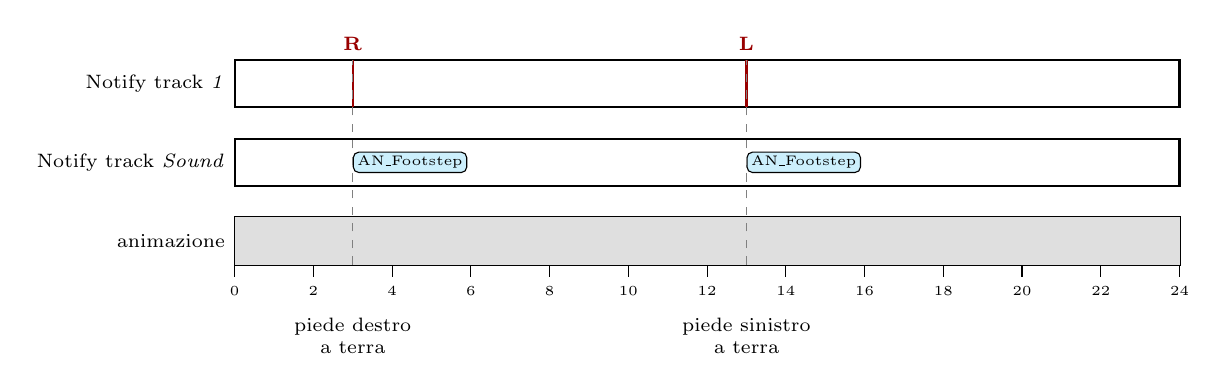
\begin{tikzpicture}[font=\footnotesize, x=0.5cm]
  \draw[thick] (0,0) rectangle (24,0.6);
  \node[left, font=\scriptsize] at (0,0.3) {Notify track \emph{1}};
  \draw[thick] (0,-1.0) rectangle (24,-0.4);
  \node[left, font=\scriptsize] at (0,-0.7) {Notify track \emph{Sound}};
  \draw[thick] (0,-2.0) rectangle (24,-1.4);
  \node[left, font=\scriptsize] at (0,-1.7) {animazione};
  \foreach \f in {0,2,...,24} {\draw (\f,-2.0) -- (\f,-2.15);
    \node[below, font=\tiny] at (\f,-2.15) {\f};}
  \fill[gray!25] (0,-2.0) rectangle (24,-1.4);
  \foreach \f/\n in {3/R, 13/L} {
    \draw[red!60!black, thick] (\f,0) -- (\f,0.6);
    \node[red!60!black, font=\scriptsize\bfseries, above] at (\f,0.6) {\n};
    \node[draw, fill=cyan!20, rounded corners=2pt, font=\tiny, inner sep=1.5pt, anchor=west]
      at (\f,-0.7) {AN\_Footstep};
    \draw[dashed, gray] (\f,-2.0) -- (\f,0.6);
  }
  \node[font=\scriptsize, align=center] at (3,-2.9) {piede destro\\a terra};
  \node[font=\scriptsize, align=center] at (13,-2.9) {piede sinistro\\a terra};
\end{tikzpicture}
\caption{La linea del tempo della corsa del bot (e delle due corse inclinate). Sulla
traccia \emph{1} i Sync Marker R e L ai frame 3 e 13; su una nuova traccia \emph{Sound}
l'AN\_Footstep negli stessi due punti. La lunghezza della linea del tempo è indicativa:
il numero totale di frame dell'animazione non si sente nella trascrizione. Schema
ricostruito.}
\label{ue10:fig:track}
\end{figure}

\paragraph{Approfondimento: Sync Marker, Blend Space e Notify doppi.} I Sync Marker non
sono legati alle ossa, come la trascrizione può far pensare, ma alla linea del tempo:
sono etichette con un nome (qui R e L) che segnano le fasi del passo. Servono quando
Unreal deve mescolare animazioni di durata diversa, nei Blend Space o con i
\emph{Sync Group}: invece di allinearle per tempo normalizzato, le allinea per marker, in
modo che i piedi tocchino terra insieme in tutte le animazioni mescolate. Funziona solo se
tutte le animazioni hanno gli stessi marker, con gli stessi nomi: è il motivo pratico per
cui il docente li aggiunge a tutte e tre le corse. I Notify, invece, pongono una domanda
diversa: in un Blend Space che sta mescolando tre animazioni, \emph{di quale} animazione
devono scattare i Notify? Nei Details del Blend Space, nella sezione \emph{Animation
Notifies}, l'opzione \emph{Notify Trigger Mode} decide: \emph{All Animations} (tutte quelle
che hanno un peso, con il rischio di sentire due o tre passi sovrapposti),
\emph{Highest Weighted Animation} (solo quella che pesa di più, la scelta più sicura per i
passi) o \emph{None}. Da notare infine che, nella lezione, la camminata a 250 non riceve
il Notify: a velocità intermedie i passi si sentono solo se il campione dominante è una
delle corse; per un risultato completo va aggiunto anche alla camminata, ai suoi frame di
appoggio. L'editor delle animazioni offre anche un Notify già pronto,
\emph{Play Sound}, che suona un suono senza Blueprint (il suo limite è che non sa
distinguere le superfici), e i \emph{Notify State}, che hanno un inizio e una fine invece
di un istante.

% ---------------------------------------------------------------------
\section{I Physical Material e le pedane}
\label{ue10:sec:physmat}

``Adesso, se noi andiamo in play, andiamo a vedere. Guardate un po'.'' A ogni passo
compare il trace che identifica il terreno, ``in questo caso il terreno di default''. ``Ma
come facciamo a dire, guarda, questo è un terreno diverso da quello normale? Dobbiamo
usare i Physics Material.''

\paragraph{Creare i Physical Material.} Una cartella \textbf{PhysicsMaterial} (``eccola
qua''); dentro, tasto destro, \textbf{Physics} $\rightarrow$ \textbf{Physical Material}. Se
ne creano due: \textbf{PM\_Rock} e \textbf{PM\_Water}. Poi, ``una cosa molto semplice,
ragazzi'': doppio clic su ciascuno; c'è la proprietà \textbf{Surface Type}, che di default
vale \emph{Default}: per PM\_Water si sceglie \textbf{Water}, per PM\_Rock \textbf{Rock}.
I nomi sono quelli scritti nelle Project Settings (figura~\ref{ue10:fig:catena}).

\paragraph{Le pedane.} ``L'unica cosa che ci manca è prendere una qualsiasi superficie.'' Un
blocco del livello, clonato (\textbf{Alt} più trascinamento, o duplicato) e schiacciato:
``fate un pianerottolino piccoletto'', due pedane. ``Adesso non abbiamo i materiali, ad
esempio, dell'acqua e della terra, ma ne mettiamo due a caso'': un materiale \emph{solid
blu} per l'acqua, \emph{Boulder} per la roccia; sono solo un segnale visivo. Poi:
selezionata la Static Mesh, ``andiamo giù, giù, giù, fino a trovare il \textbf{Phys
Material Override}'', e lì \textbf{PM\_Water} per l'acqua, \textbf{PM\_Rock} per la
roccia. ``Adesso, se noi andiamo sopra con il character, sentiamo che'' sulla roccia il
passo cambia. ``Eccolo qua.''

\begin{figure}[htbp]
\centering
\begin{tikzpicture}[font=\footnotesize,
  ue10box/.style={draw, thick, rounded corners=4pt, align=center, fill=gray!8,
                 minimum height=1.1cm, text width=2.5cm},
  ue10arr/.style={-{Stealth[length=2.5mm]}, thick}]
  \node[ue10box, fill=blue!8] (ps) at (0,0) {\textbf{Project Settings}\\{\scriptsize
    Engine, Physics, Physical Surface: Rock, Water}};
  \node[ue10box, fill=orange!12] (pm) at (4.3,0) {\textbf{PM\_Rock}, \textbf{PM\_Water}\\
    {\scriptsize Physical Material, Surface Type}};
  \node[ue10box, fill=green!10] (sm) at (8.6,0) {\textbf{Pedana}\\{\scriptsize Static
    Mesh, Phys Material Override}};
  \node[ue10box, fill=yellow!15] (tr) at (12.9,0) {\textbf{AN\_Footstep}\\{\scriptsize
    trace, Hit Result, Get Surface Type, Switch}};
  \node[ue10box, fill=violet!12] (cue) at (12.9,-2.4) {\textbf{Sound Cue}\\{\scriptsize
    Footstep, Rock, Water}};
  \node[ue10box, fill=red!10] (an) at (8.6,-2.4) {\textbf{Animazioni di corsa}\\
    {\scriptsize Notify ai frame 3 e 13}};
  \draw[ue10arr] (ps) -- node[above, font=\scriptsize]{nomi} (pm);
  \draw[ue10arr] (pm) -- node[above, font=\scriptsize]{assegnato} (sm);
  \draw[ue10arr] (sm) -- node[above, font=\scriptsize]{colpita} (tr);
  \draw[ue10arr] (tr) -- node[right, font=\scriptsize]{sceglie} (cue);
  \draw[ue10arr] (an.north east) -- node[below right, font=\scriptsize, pos=0.4]{fa
    scattare} (tr.south west);
\end{tikzpicture}
\caption{La catena completa dei passi. I nomi delle superfici nascono nelle Project
Settings, vengono assegnati ai Physical Material, che a loro volta si assegnano alle
superfici del livello; a ogni passo, il Notify inserito nell'animazione lancia il trace,
legge la superficie colpita e sceglie il Sound Cue. Schema ricostruito.}
\label{ue10:fig:catena}
\end{figure}

\paragraph{La spiegazione ripetuta.} A uno studente che chiede dove trovare ``i cosini''
(i PM): ``quelli li crei, praticamente. Lo fai con tasto destro, Physics, Physical
Material, e lo crei. Lo chiami PM\_Rock, come vuoi, PM\_Rock e PM\_Water. Ci clicchi su
ognuno di essi e gli cambi il Surface Type: lo metti Rock per il rock e Water per il
water. Poi, fatto questo, prendi un qualsiasi asset (vabbè, anche un blocco va
benissimo): devi andare su Phys Material Override e gli metti il Physical Material.''
``Basta che fai due pedanine'': ``qualsiasi superficie che tu vuoi prendere, ci puoi
camminare sopra''; ``la scali, fai quello che vuoi, fondamentalmente''.

\paragraph{Approfondimento: dove si assegna un Physical Material.} Il \emph{Phys Material
Override} usato a lezione vale per tutto il componente: comodo per una pedana, poco
pratico per un terreno che cambia da un punto all'altro. Unreal offre altri due posti. Il
primo è il \textbf{materiale}: nei Details di un Material (o di un Material Instance) c'è
la proprietà \emph{Phys Material}; tutte le mesh che usano quel materiale ``diventano''
roccia o acqua, senza toccare il livello, ed è la soluzione abituale nei progetti veri.
Il secondo è il \textbf{Landscape}: ogni layer dipinto può avere il suo Physical Material,
e il trace legge quello del layer dominante nel punto colpito. In più, il Physical
Material non serve solo ai suoni: contiene l'attrito (\emph{Friction}), il rimbalzo
(\emph{Restitution}) e la densità usati dalla simulazione fisica, ed è la base per gli
effetti d'impatto dei proiettili (scintille sul metallo, polvere sulla pietra), con la
stessa tecnica del Get Surface Type e dello Switch.

% ---------------------------------------------------------------------
\section{Gli ultimi problemi e la chiusura}
\label{ue10:sec:chiusura}

\paragraph{Gli ultimi problemi.} ``Un attimo: è successo un casino? Gli altri? Qualche
problema? Funziona?''
\begin{itemize}
  \item Uno studente si è perso il primo pezzo del grafo dell'AN\_Footstep e non sa da
        dove vengano Mesh Comp, Animation ed Event Reference: sono gli ingressi di
        Received\_Notify, la funzione sovrascritta con \emph{Override}. Poi, di nuovo, la
        catena: ``Get Owner, Get Actor Location, Get Actor Up Vector, e poi sottrai,
        per far sì che'' End sia sotto lo Start, ``che è il Get Actor Location''.
  \item Lo stesso studente ha messo le pedane, ma il personaggio non fa nessun rumore,
        nemmeno sul pavimento normale. I suoni nell'Anim Notify ci sono (``Rock1, Water
        Cue, Footstep Cue: va benissimo''); l'errore è nel vettore: il Get Actor Up Vector
        era collegato al pin sbagliato del Multiply. ``Mettilo sopra; stacca quello
        sotto; tasto destro su quello là, to float, 250.'' Con il Draw Debug Type a For
        Duration e una ricompilazione, il passo si sente.
  \item Le pedane, però, non fanno il suono della roccia: ``fammi vedere se hai messo la
        cosa'', e infatti il Phys Material Override non c'era. Lo studente non riesce a
        scendere nei Details fino alla voce: il pannello era filtrato su una categoria
        (\emph{Generale}); cliccando su \emph{Tutto} e aprendo la parte avanzata della
        sezione \emph{Physics} (``vai su tutto, clicca su tutto; giù, eccolo là''), si
        trova \emph{Phys Material Override}. ``A posto, perfetto.''
  \item ``A me non compaiono le linee'': ``basta che fai Draw Debug Type e la metti For
        Duration'', sul Line Trace By Channel. ``Quello è solo una cosa di debug,
        tranquilli.''
\end{itemize}

\paragraph{L'inclinazione rimandata.} ``Io ho sempre quella cosa dell'inclinazione della
testa'': è la studentessa del Lean che non inclina. ``Possiamo farlo la prossima volta?''
``Sì, facciamo la prossima volta. Tanto la prossima volta facciamo interazioni, e allora
ricordamelo tu, eh?'' ``Così fixiamo tutto''; ``lo guardo poi in futuro, lo guardo poi in
post anche''.

\paragraph{Il calendario.} ``Io vi ringrazio per l'attenzione, grazie'' anche a chi segue
in differita. ``Ci vediamo giovedì per la prossima lezione, che faremo in questo caso i
menu: andiamo a fare un po' di UI.'' (Il docente, poco prima, aveva parlato di
``interazioni'': dalla trascrizione non si capisce se la lezione di giovedì conterrà
entrambe le cose.) Uno studente pensava che oggi fosse giovedì; il calendario: ``abbiamo
questo martedì, giovedì e, se non sbaglio, il 30, che è martedì prossimo: è l'ultima con
me. Poi ci avete Davide.'' ``Va bene, ragazzi. Allora ci vediamo. Buona cena. Buona
serata.''

\begin{table}[htbp]
\centering
\small
\begin{tabular}{@{}p{5.4cm}p{8.6cm}@{}}
\toprule
\textbf{Sintomo} & \textbf{Causa e rimedio} \\
\midrule
Il personaggio non si muove, errori su IA\_Run & IA\_Move cancellata e sostituita da
IA\_Run: duplicare IA\_Look (Vector 2D), rinominarla IA\_Move, rimetterla in IMC\_Default
e nell'evento \\
L'evento del movimento non mostra il vettore & salvare l'Input Action; poi Split Struct
Pin sull'Action Value \\
Dopo una compilazione ``sparisce tutto'' & il Blueprint non compila: leggere i Compiler
Results \\
Camera storta, movimento strano & Spring Arm attaccato alla freccia o spostato dal pivot:
riattaccarlo, location a zero, usare Target Arm Length, Socket Offset, Target Offset \\
La camera non segue il mouse & Use Pawn Control Rotation sullo Spring Arm \\
La torretta ignora il nuovo personaggio & manca il tag Player; controllare le risposte
ai trace e alle collisioni \\
Il Montage non si vede & manca lo Slot DefaultSlot nell'AnimGraph \\
Durante il Montage il corpo gira & il DefaultSlot prende tutte le ossa: serve uno slot
per la parte alta (Layered blend per bone) \\
Errori nell'Event Graph incollato & variabili del vecchio ABP: ricrearle con Create
variable, rifare le referenze nell'Initialize \\
\emph{Idle to Walk will never be taken} & la regola della transizione non è ancora
scritta \\
Lo stato non mostra l'anteprima del Blend Space & lo stato non è mai raggiunto
(transizione o dati mancanti) \\
Il personaggio levita & Mesh a Z = $-90$ \\
Il personaggio si muove in T-pose & State Machine non collegata all'Output Pose, o
Mesh senza Anim Class \\
Errori su Jump e Fall & regole vuote: Automatic Rule Based on Sequence Player in State, e
la regola Fall $\rightarrow$ Land Run \\
GroundSpeed sempre zero & due variabili Character Movement (una mai valorizzata), o
Update non collegato al Validated Get \\
Il Lean non inclina & segno e scala del Delta Rotator, opzioni di rotazione; rimandato
alla lezione successiva \\
La camera inclinata di lato & ruotata sulla X (Roll) invece che sulla Y (Pitch) \\
AN\_Footstep non compare in Add Notify & la classe ha un altro nome: cercarla con quello
\\
Nessun suono di passi & Up Vector sul pin sbagliato del Multiply; Notify non inserito
nelle animazioni \\
Le pedane suonano come il pavimento & manca il Phys Material Override, o il Surface Type
del Physical Material \\
Phys Material Override introvabile & filtro dei Details su Generale: scegliere Tutto e
aprire le opzioni avanzate \\
Le linee del trace non si vedono & Draw Debug Type a For Duration \\
\bottomrule
\end{tabular}
\caption{I problemi incontrati durante la lezione, con la causa e il rimedio.}
\label{ue10:tab:errori}
\end{table}

\begin{table}[htbp]
\centering
\small
\begin{tabular}{@{}p{4.8cm}p{9.2cm}@{}}
\toprule
\textbf{Nodo, asset o impostazione} & \textbf{Che cosa fa} \\
\midrule
Input Action, Value Type Vector 2D & azione con un valore a due assi (movimento,
sguardo) \\
Add Movement Input & muove il Pawn lungo una direzione, con una scala \\
Tags (Actor) & etichette con cui altri Blueprint riconoscono l'actor \\
Try Get Pawn Owner / Cast To & il Pawn che possiede l'animazione; la sua classe precisa \\
Promote to Variable & salva un'uscita in una nuova variabile \\
Convert to Validated Get & Get con controllo di validità (Is Valid / Is Not Valid) \\
Create variable (tasto destro) & crea la variabile mancante di un nodo incollato \\
Comment (tasto C) / Reroute Node (doppio clic sul filo) & riquadro con titolo; punto di
piegatura di un filo \\
Blend Space 2D: Lean e GroundSpeed & mescola le corse inclinate e la camminata \\
Get Owning Actor / Get Actor Rotation & l'actor proprietario; la sua rotazione \\
Delta Rotator & la differenza normalizzata fra due rotazioni \\
FInterp To / RInterp To & un passo d'interpolazione fra float; fra rotator \\
Get World Delta Seconds & il tempo dell'ultimo frame \\
State Machine, Can Enter Transition & stati e regole booleane di passaggio \\
Automatic Rule Based on Sequence Player in State & la transizione scatta a fine
animazione \\
AND Boolean / NOT Boolean & congiunzione; negazione \\
Get Last Input Vector & l'ultimo input di movimento del Pawn (lunghezza 0--1) \\
Vector Length & la lunghezza di un vettore \\
Print String & scrive un valore a schermo, per il debug \\
World Settings: Default Pawn Class & il personaggio del giocatore nel livello \\
Anim Notify (classe), Received\_Notify & evento in un istante dell'animazione; la funzione
che lo riceve \\
Get Owner / Get Actor Location / Get Actor Up Vector & proprietario; posizione; vettore
verso l'alto \\
Line Trace By Channel, Draw Debug Type & trace lungo un segmento; disegno di debug \\
Break Hit Result: Impact Point & il punto esatto dell'impatto \\
Get Surface Type & il tipo di superficie colpita (dal Physical Material) \\
Physical Surface (Project Settings) & i nomi dei tipi di superficie \\
Switch on EPhysicalSurface & un'uscita per ogni tipo di superficie \\
Play Sound at Location & suona un suono in un punto \\
Sound Wave / Sound Cue & file audio; grafo che combina e modula i suoni \\
Create Single Cue & crea un Cue dai Sound Wave selezionati (con Random) \\
Random / Modulator & sceglie un ingresso a caso; varia pitch e volume \\
Add Sync Marker & marcatore con nome sulla linea del tempo (R, L) \\
Insert Notify Track / Add Notify & nuova traccia di Notify; inserisce un Notify \\
Physical Material: Surface Type & il tipo di superficie dell'asset \\
Phys Material Override & assegna un Physical Material a un componente \\
\bottomrule
\end{tabular}
\caption{I nodi, gli asset e le impostazioni della decima lezione.}
\label{ue10:tab:nodi}
\end{table}

% ---------------------------------------------------------------------
\section*{Punti chiave del capitolo}
\addcontentsline{toc}{section}{Punti chiave del capitolo}

\begin{itemize}
  \item Un'\textbf{Input Action} cancellata rompe il personaggio in modo silenzioso: si
        ricrea duplicando un'azione dello stesso tipo (\textbf{IA\_Look}, Vector 2D, per
        \textbf{IA\_Move}), la si rimette nell'\textbf{IMC} e nell'evento. Lo
        \textbf{Spring Arm} non si sposta dal pivot: si regolano Target Arm Length,
        Socket Offset e Target Offset.
  \item Quando si cambia personaggio, tutto ciò che riconosceva il vecchio va
        ricontrollato: \textbf{tag} (Player per la torretta), \textbf{cast} a classi
        precise, \textbf{collisioni} e risposte ai trace.
  \item Un Animation Blueprint si può costruire \textbf{copiando} l'Update di un altro, ma
        l'\textbf{Initialize} si rifà: Try Get Pawn Owner, Cast To, referenze promosse a
        variabile, ``un gancio'' fra animazione e personaggio. Le variabili mancanti si
        ricreano con \textbf{Create variable}; il \textbf{Validated Get} protegge l'Update.
        Attenzione alle variabili doppie (Character Movement 0).
  \item Ordine nel grafo: \textbf{commenti} con il tasto C, \textbf{Reroute} con un doppio
        clic sul filo.
  \item Il \textbf{Blend Space 2D} del bot ha il \textbf{Lean} in orizzontale ($-10$,
        10) e la \textbf{GroundSpeed} in verticale (0--500, la Max Walk Speed): corsa e
        corse inclinate a 500, camminata a 250, nessun Idle.
  \item Il \textbf{Lean} si calcola a ogni frame: rotazione attuale, \textbf{Delta
        Rotator} con quella precedente, lo \textbf{Yaw}, \textbf{FInterp To} verso quel
        valore (Interp Speed 1--5, Get World Delta Seconds), poi la rotazione attuale
        diventa la precedente. Segno e scala vanno verificati.
  \item La \textbf{State Machine} ha sette stati: Idle e Walk (GroundSpeed $>$ 0, $\le$
        0), Jump Idle e Jump Run (IsFalling AND la velocità), Fall (automatica dopo i
        salti), Land Idle e Land Run (NOT IsFalling AND [NOT] \textbf{ReceiveInput}),
        ritorni automatici. ReceiveInput viene da \textbf{Get Last Input Vector}: la
        lunghezza maggiore di zero dice che il giocatore sta premendo.
  \item Per giocare con il bot: Spring Arm e Camera a zero, Target Offset, \textbf{Default
        Pawn Class} nelle World Settings, i grafi di input copiati dal vecchio
        personaggio, Use Pawn Control Rotation, Mesh a $-90$.
  \item I passi: un \textbf{Anim Notify} (AN\_Footstep, \textbf{Received\_Notify}) lancia
        un \textbf{Line Trace By Channel} di 250 centimetri verso il basso; dal Hit Result,
        \textbf{Get Surface Type} e \textbf{Switch on EPhysicalSurface} scelgono il
        \textbf{Play Sound at Location} sull'\textbf{Impact Point}.
  \item I tipi di superficie si definiscono nelle \textbf{Project Settings} (Physics,
        Physical Surface: Rock, Water); i \textbf{Physical Material} (PM\_Rock, PM\_Water)
        li assegnano con il Surface Type; il \textbf{Phys Material Override} li applica
        alle mesh del livello.
  \item I \textbf{Sound Cue} variano i passi: \textbf{Random} fra più Sound Wave
        (\emph{Create Single Cue}) e \textbf{Modulator} sul pitch (passo 0,95--1,3, roccia
        2--2,2, acqua 1,3--1,5).
  \item Nelle animazioni di corsa: \textbf{Sync Marker} R e L e una \textbf{Notify Track}
        \emph{Sound} con l'AN\_Footstep ai frame di appoggio (3 e 13), in tutte e tre le
        animazioni.
\end{itemize}

%
%  Tutte le etichette di questo capitolo hanno il prefisso "ue10:"
%  (ue10:cap:..., ue10:sec:..., ue10:fig:..., ue10:tab:...), e tutti gli
%  stili TikZ hanno il prefisso "ue10" (ue10node, ue10exec, ue10data,
%  ...) per non collidere con chiavi native di TikZ né con quelli delle
%  lezioni precedenti. Il capitolo è autonomo: non contiene \ref verso
%  altri capitoli (i rimandi alle lezioni precedenti sono a parole).
%  Le figure sono ricostruzioni schematiche di quanto mostrato e detto a
%  lezione, non copie delle schermate del docente. Dove la trascrizione
%  è troppo rovinata per ricostruire un dettaglio, il capitolo lo dice
%  invece di inventarlo.
% =====================================================================

\chapter[Lean, State Machine e Physical Material]{Il nuovo personaggio: Lean,
State Machine e passi con i Physical Material}
\label{ue10:cap:bot}

Questa è la \textbf{decima lezione} del corso breve di \textbf{introduzione a Unreal
Engine}. Alla fine della nona il docente aveva lasciato un compito facoltativo: costruire
da zero un personaggio nuovo con lo \textbf{StackOBot}, il robottino dei progetti di
esempio di Epic, che ha già tutte le sue animazioni. Il compito era ``molto facoltativo,
perché capisco che è complicato''; in questa lezione lo si fa insieme, dall'inizio alla
fine: ``faremo proprio un nuovo character, che useremo poi come default''.

Il nuovo personaggio riprende la struttura del cavaliere della lezione precedente
(Animation Blueprint, State Machine, Blend Space), ma con tre differenze che danno il
titolo al capitolo. La prima è il \textbf{Lean}: il bot non ha otto animazioni
direzionali, ma una corsa e due varianti \emph{inclinate}, verso sinistra e verso
destra; il Blend Space 2D non usa più la direzione, ma un valore d'inclinazione calcolato
a ogni frame dalla differenza fra la rotazione attuale e quella del frame precedente. La
seconda è una \textbf{State Machine} più ricca, a sette stati, che distingue il salto da
fermo dal salto in corsa e l'atterraggio da fermo dall'atterraggio in movimento, con una
nuova variabile che dice se il giocatore sta premendo un tasto di movimento. La terza è
il suono dei \textbf{passi}: un \textbf{Anim Notify} inserito nelle animazioni, nel
momento esatto in cui il piede tocca terra, lancia un \emph{line trace} verso il basso,
legge il tipo di superficie colpita e suona il passo giusto; le superfici si distinguono
con i \textbf{Physical Material}, ``i materiali che possono determinare uno stato fisico''
di un oggetto. Sulla roccia si sente la roccia, sull'acqua l'acqua, altrove il passo
normale.

La lezione è \textbf{online}, su Zoom, come le precedenti. Si apre con una lunga
correzione in diretta del progetto di uno studente, prosegue con la costruzione del bot,
interrotta più volte dalle domande e dai problemi dei presenti, risolti in condivisione di
schermo, e si chiude sui passi e i Physical Material. La pausa arriva dopo la variabile
dell'input (``ci vediamo alle solite 18. Scusate: 17.55''); alla fine, ``vi mando a
cena''. È una lezione di \emph{fine corso}: ``mancano tre lezioni alla fine'', e il
docente lo ricorda per invitare chi segue in differita a entrare in diretta, se vuole
correzioni dal vivo.

Tre avvertenze di lettura, le stesse delle lezioni precedenti. La prima: la trascrizione
è automatica e storpia moltissimi nomi. Unreal è ``Arreal'', ``ArRIAL'', ``a Real'' e
``Arriva''; il \textbf{Lean} è ``Lin'', ``Line'', ``l'in'', ``LIN'' e ``Linn'' (``l'in è il
piegamento della rotazione''); l'\textbf{Idle} è ``idol'' e ``Idol''; l'\textbf{Event
Graph} è ``even graph'', ``Even Graph'' e ``Vengraph''; l'\textbf{AnimGraph} è
``Alimgraph'', ``aningraf'' e ``Aningraft''; \textbf{IA\_Move} è ``IAMove'', ``iam
move'', ``Iammov'' e ``gli ammove''; \textbf{IA\_Run} è ``iaran'', ``IRRun'' e ``iarran'';
l'\textbf{IMC} è ``IAMC'' e ``negli MC''; il \textbf{Then 0} della Sequence è
``DANZIRO'' e ``den zero''; i \textbf{Reroute Node} sono ``re Routenold''; il
\textbf{Blend Space} è ``Benzes'' e ``Brennese''; il \textbf{Validated Get} è ``validate
get''; l'\textbf{FInterp To} è ``F inter2'' e ``fintech 2''; l'\textbf{RInterp To} è ``R
inter to''; l'\textbf{Is Falling} è ``his falling'' e ``ease falling''; il \textbf{Last
Input Vector} è ``Lasting Pwn Vector''; lo \textbf{Spring Arm} è ``Springarma'' e
``spring guard''; \textbf{Use Pawn Control Rotation} è ``PoundCtrlRotation'', ``Pwn
rotation'' e ``use spawn control rotation''; le \textbf{World Settings} sono ``Word
Settings'' e la \textbf{Default Pawn Class} è ``default on class''; l'\textbf{Anim
Notify} è ``an in notify'', ``Anim Notifaj'', ``modify'', ``anni nota'' e ``anni
notifà''; \textbf{AN\_Footstep} è ``a n footstep'' e ``AN full step''; il
\textbf{Physical Material} è ``fisic material'' e ``P FIS materia''; \textbf{Get Surface
Type} è ``Gethsurfest Type'' e ``get sur festival''; il \textbf{Sound Cue} è ``queue'' e
``Q''; il \textbf{Draw Debug Type} è ``drop the bug type'' e ``draw the bug type''; il
\textbf{Break Hit Result} è ``break it risult''; \textbf{BP\_Knight} è ``BP Night'' e
``Night''; il \textbf{bot} è a tratti ``Boto'' e ``voto''. Dove la ricostruzione è
sicura il capitolo usa la forma corretta; dove non lo è riporta la forma della
trascrizione e lo dice. La seconda: all'inizio della registrazione e durante la pausa il
riconoscimento vocale produce lunghi blocchi di testo senza senso e ripetuto (``grazie a
tutti per l'attenzione che ci ha spiegato'', ``qual è la risposta che ci può essere?'',
``la situazione è questa, la migliore dal 2005'', il ``rinforzare la democrazia'', la
``dottrina sul mercato del lavoro'', il ``dialogo interculturale''): non appartengono
alla lezione e sono stati ignorati. La terza: buona parte della lezione è fatta di
indicazioni a voce mentre si lavora (``vai su'', ``clicca qua'', ``attacca quello
sotto''), spesso rivolte allo schermo di uno studente; il capitolo ricostruisce i grafi
da ciò che il docente dice mentre li costruisce, distingue i tentativi dalle soluzioni,
completa i nomi esatti dei nodi e dei pin di Unreal Engine 5, e dichiara i punti in cui
la trascrizione lascia un buco.

\paragraph{Come leggere questo capitolo.} Il capitolo segue l'ordine della lezione. Le
figure ricostruiscono il movimento riparato con l'Enhanced Input, i due eventi
dell'Animation Blueprint del bot con il Validated Get, il calcolo del Lean, il Blend
Space 2D del bot, la State Machine a sette stati, il grafo dell'Anim Notify dei passi, la
catena che porta dalla superficie al suono, il Sound Cue con Random e Modulator, e la
linea del tempo dell'animazione di corsa con i Sync Marker e i Notify. Le tabelle
riassumono le transizioni della State Machine, i valori dei Sound Cue, gli errori
incontrati durante la lezione e i nodi della giornata. Qua e là, dei paragrafi di
\textbf{approfondimento} collegano la lezione ai libri di Marcos Romero e Brenden Sewell
(\emph{Blueprints Visual Scripting for Unreal Engine 5} e la seconda edizione dello
stesso testo, scritta per Unreal Engine 4), i testi di riferimento per questa parte del
libro, e a qualche nozione tecnica generale su Unreal Engine 5; sono segnalati come tali
e non fanno parte della lezione.

Il percorso del capitolo:
\begin{enumerate}
  \item l'\textbf{inizio della lezione}: il movimento e la camera riparati in diretta
        (sezione~\ref{ue10:sec:riparazione});
  \item gli \textbf{annunci} e le domande: i passi e i Physical Material, il compito
        facoltativo, il personaggio nuovo che non interagisce con il livello, la lezione
        di giovedì, il bot di Federico (sezioni \ref{ue10:sec:annunci}
        e~\ref{ue10:sec:federico});
  \item il \textbf{risultato finale}, mostrato in anteprima
        (sezione~\ref{ue10:sec:demo});
  \item il nuovo personaggio: \textbf{Animation Blueprint} e \textbf{Blueprint
        Character}, l'Event Graph copiato, l'\textbf{Initialize} e il \textbf{Validated
        Get}, commenti e Reroute (sezioni da~\ref{ue10:sec:abp}
        a~\ref{ue10:sec:commenti});
  \item il \textbf{Blend Space 2D} del bot e il calcolo del \textbf{Lean} (sezioni
        \ref{ue10:sec:blend} e~\ref{ue10:sec:lean});
  \item la \textbf{State Machine} a sette stati, la variabile dell'\textbf{input} e le
        regole di transizione, prima e dopo la pausa (sezioni da~\ref{ue10:sec:sm}
        a~\ref{ue10:sec:transizioni2});
  \item il bot \textbf{in gioco}, con la camera, e il debug dei progetti degli studenti
        (sezioni \ref{ue10:sec:ingioco} e~\ref{ue10:sec:debug});
  \item i \textbf{passi}: l'\textbf{Anim Notify}, il \emph{line trace}, i
        \textbf{Physical Surface}, i \textbf{Sound Cue}, i \textbf{Notify} nelle
        animazioni e i \textbf{Physical Material} (sezioni da~\ref{ue10:sec:notify}
        a~\ref{ue10:sec:physmat});
  \item gli ultimi problemi e la \textbf{chiusura}
        (sezione~\ref{ue10:sec:chiusura}).
\end{enumerate}

% ---------------------------------------------------------------------
\section{Prima della lezione: il movimento da riparare}
\label{ue10:sec:riparazione}

Dopo i minuti iniziali di rumore della trascrizione, i saluti (``buongiorno, buon
pomeriggio'') e una prima richiesta. Mentre gli altri ``stanno ancora entrando'', uno
studente racconta il suo problema: ha seguito la lezione precedente in differita (``ho
seguito la lezione da quando è stata salvata''), e all'inizio ``andava tutto, si
muoveva''; poi, a un certo punto, il personaggio non si muoveva più, e ``la camera,
anche se segnata, non c'è, ed è sparito tutto''. Il docente propone di risolverlo subito
(``tanto adesso stanno ancora entrando'') e la correzione si fa in condivisione di
schermo. È una sequenza lunga e caotica, ma istruttiva: mostra come si legge un errore di
compilazione e come si ricostruisce un pezzo di Enhanced Input perduto.

\paragraph{Leggere gli errori.} ``Già ti dico che comunque possiamo già vedere gli
errori là sotto'': il pannello dei risultati della compilazione (\emph{Compiler
Results}) in fondo all'editor del Blueprint elenca i nodi che non trovano più ciò a cui
si riferiscono. La prima diagnosi, a colpo d'occhio: ``sicuramente ti manca
l'\emph{Input Action}''. L'errore dice che l'evento di \textbf{IA\_Run} non esiste più
nel nodo, o che il contesto \textbf{IMC\_Default} non lo contiene: ``dice che
fondamentalmente non hai IA\_Run: l'hai cancellato per sbaglio oppure non l'hai mai
creato?''. In realtà IA\_Run c'è (``il Content Browser, fai IA\_Run, ed eccolo là''): il
problema è un altro.

\paragraph{IA\_Move cancellata.} Aprendo l'\textbf{IMC\_Default} (``scrivi IMC, invece di
IAMC''), il docente trova dei mapping che lo studente non ricorda di aver messo (``ma no,
non li ho messi io''): li si cancella tutti con il cestino, poi si torna indietro con
\textbf{Ctrl+Z} (``fai Ctrl+Z a tutti, va benissimo''). Guardando il mapping che dovrebbe
essere \textbf{IA\_Move} si capisce: ``hai cancellato IA\_Move, fondamentalmente'', e al
suo posto, nell'Event Graph, l'evento del movimento è stato sostituito da IA\_Run (``ah,
perché l'hai sostituito''). ``E devi stare attento a queste cose.''

\paragraph{Ricreare IA\_Move.} ``La cosa che devi fare adesso è praticamente ricreare
IA\_Move.'' Il primo istinto è duplicare IA\_Run; poi il docente si corregge: ``no, no,
no: fai un doppione di \textbf{IA\_Look}''. Il motivo è il tipo di valore: IA\_Run è un
booleano (\emph{Digital}), mentre il movimento, come lo sguardo, è un \textbf{Vector 2D}
(``è un Vector 2D''): duplicare IA\_Look dà un'azione già del tipo giusto. Il doppione si
rinomina \textbf{IA\_Move}. Poi, nell'IMC\_Default:
\begin{itemize}
  \item si rimette IA\_Move nel mapping che lo usava prima (``adesso segnali negli MC
        quello di prima, IA\_Move'');
  \item con il \textbf{più} in alto si crea un altro mapping, per \textbf{IA\_Run}: con la
        freccina sotto il nome si apre la scelta del tasto e, invece di cercarlo nella
        lista, ``basta che clicchi sulla tastiera: clicca Shift sulla tua tastiera''. Il
        campo del tasto, quando è in ascolto, registra il primo tasto premuto.
\end{itemize}
Una compilazione di prova: ``qualche cosa si è levato, benissimo''.

\paragraph{L'evento e gli Add Movement Input.} Restano gli errori nell'Event Graph del
personaggio (il cavaliere, ``Knight''): ``hai sostituito IA\_Move con IA\_Run: devi levare
questo e mettere IA\_Move''; con il tasto destro si ricrea l'evento \textbf{IA\_Move}.
Uno strano dettaglio (``strano che non ti fa vedere'') si risolve salvando l'azione: solo
dopo il salvataggio l'evento mostra l'\textbf{Action Value} come vettore 2D. Si ricostruisce
il grafo del movimento, quello copiato la volta precedente dal ThirdPersonCharacter:
\begin{enumerate}
  \item tasto destro sull'\textbf{Action Value} e \textbf{Split Struct Pin}, per avere i
        pin \textbf{X} e \textbf{Y} separati;
  \item la \textbf{X} si collega al primo \textbf{Add Movement Input}, la \textbf{Y}
        ``tutto dritto fino a Scale Value del successivo'';
  \item il secondo Add Movement Input era stato cancellato (``ah, non c'è''): lo si
        ricopia dal primo (``copia Add Movement Input'');
  \item nella \textbf{World Direction} si collega ``quel forward vector che c'è lì
        vicino, quello arancione'' (il vettore di direzione calcolato dalla rotazione
        del controller);
  \item infine il pin di esecuzione: dal \textbf{Triggered} di IA\_Move, ``attacchi
        tutto in sequenza''.
\end{enumerate}
``E abbiamo riparato il movimento'' (figura~\ref{ue10:fig:move}). Compilato, il
personaggio si muove.

\begin{figure}[htbp]
\centering
\begin{tikzpicture}[font=\footnotesize,
  ue10node/.style={draw, thick, rounded corners=4pt, align=center, fill=gray!8,
                  minimum height=0.9cm, text width=3.4cm},
  ue10ev/.style={ue10node, fill=red!12},
  ue10exec/.style={-{Stealth[length=2.5mm]}, very thick, black!80},
  ue10data/.style={-{Stealth[length=2mm]}, thick, blue!60!black}]
  \node[ue10ev, text width=2.6cm, minimum height=2.0cm] (ev) at (0,0)
    {\textbf{IA\_Move}\\{\scriptsize Enhanced Input Action}\\{\scriptsize Action Value
    (Vector 2D), split in X e Y}};
  \node[ue10node] (a1) at (5.0,0.9) {\textbf{Add Movement Input}\\
    {\scriptsize World Direction: vettore destro; Scale Value: X}};
  \node[ue10node] (a2) at (10.0,0.9) {\textbf{Add Movement Input}\\
    {\scriptsize World Direction: vettore avanti; Scale Value: Y}};
  \node[ue10node, fill=green!10, text width=4.2cm] (rot) at (7.5,-1.9) {Get Control
    Rotation (solo lo Yaw) $\rightarrow$ vettori \textbf{Forward} e \textbf{Right}};
  \draw[ue10exec] (ev.east |- a1) -- node[above, font=\scriptsize]{Triggered} (a1);
  \draw[ue10exec] (a1) -- (a2);
  \draw[ue10data] (rot.west) -| node[pos=0.75, left, font=\scriptsize]{Right}
    (a1.south);
  \draw[ue10data] (rot.east) -| node[pos=0.75, right, font=\scriptsize]{Forward}
    (a2.south);
  \draw[ue10data, dashed] (ev.south) |- node[pos=0.75, below, font=\scriptsize]{X
    $\rightarrow$ Scale Value del primo, Y $\rightarrow$ Scale Value del secondo}
    (rot.south west);
\end{tikzpicture}
\caption{Il movimento riparato. L'Action Value di IA\_Move, un Vector 2D, viene diviso in
X e Y: la X muove lungo il vettore destro, la Y lungo quello in avanti, entrambi ricavati
dalla rotazione del controller. Se IA\_Move viene cancellata o sostituita da un'azione
booleana (IA\_Run), l'Action Value non è più un vettore e il grafo si rompe. Schema
ricostruito dal grafo standard del ThirdPersonCharacter; l'ordine esatto delle due
direzioni a lezione non si sente.}
\label{ue10:fig:move}
\end{figure}

\paragraph{Perché ``sparisce tutto''.} Lo studente aveva notato che a volte il
personaggio compariva e a volte, dopo una compilazione, ``proprio scompariva tutto''.
``È normale'': quando la compilazione di un Blueprint fallisce, Unreal ``te lo fa capire
in modo molto più palese'': l'icona del pulsante \emph{Compile} diventa rossa, con un
simbolo d'errore (``un'iconcina''), e un Blueprint che non compila non si comporta come
dovrebbe in gioco.

\paragraph{La camera storta.} In Play il movimento funziona, ma ``è un po' strano'', e la
camera è ``molto storta''. Tre correzioni, nell'ordine:
\begin{enumerate}
  \item \textbf{Use Pawn Control Rotation}: selezionato lo \textbf{Spring Arm}, si cerca
        ``control rotation'' e si mette la spunta (``mettilo true, perfetto''): la
        telecamera segue il controller.
  \item \textbf{La gerarchia}: la camera era stata agganciata alla \emph{freccia}
        (l'\emph{Arrow Component} del Character): ``attenzione a fare queste cose''. Lo
        Spring Arm va staccato dalla freccia e attaccato al suo posto; la Camera ``deve
        rimanere'' figlia dello Spring Arm.
  \item \textbf{La posizione}: lo Spring Arm era stato spostato con il \emph{pivot}
        (``l'hai spostato sulla location''): ``devi mettere tutto a zero''. Accanto ai
        valori della Location, nei Details, c'è una freccina circolare tutta a destra che
        li riporta al default.
\end{enumerate}
La regola, ripetuta: lo Spring Arm e la Camera non si muovono dal pivot, ``perché se no
si rompe tutto''. Per spostare la camera si usano solo i valori dello Spring Arm:
\textbf{Target Arm Length}, \textbf{Socket Offset} e \textbf{Target Offset}. ``Se muovi
il pivot, ti cambia la location del braccio, quindi ti fa tutto un effetto strano anche
con la camera.'' Siccome lo studente voleva una visuale più alta: \textbf{Target Offset},
Z (``l'ultima a destra'') a \textbf{60}. ``E già la telecamera dovrebbe essersi fissata
più o meno'': ``abbastanza bene''.

\paragraph{Le animazioni del giorno prima.} Lo studente aveva fatto anche ``la roba delle
animazioni'' (``oddio, è un po' buggato''), ma senza poterla provare, perché il
personaggio era fermo. ``Tanto oggi la riprenderemo'': si rifarà un personaggio ``proprio
da capo''.

% ---------------------------------------------------------------------
\section{Gli annunci e le domande}
\label{ue10:sec:annunci}

\paragraph{La cartella Footstep Sounds.} ``Oggi andremo a vedere anche una cosettina
interessante.'' Il docente l'ha scritto su Discord: nella cartella del materiale
didattico, su Drive, c'è una cartella \textbf{Footstep Sounds}; va scaricata e
decompressa, ``lasciatela là'', servirà più tardi. Servirà per i \textbf{Physical
Material}, ``cioè praticamente i materiali che possono determinare uno stato fisico, ad
esempio di un oggetto'': ``se un oggetto è di metallo, come deve reagire in certi
ambiti''. Oggi li si usa per i passi: ``quando lui fa superficie acquosa si sentirà il
rumore dei passi dell'acqua, se no si sentirà il rumore dei passi della roccia, o si
sentirà il rumore dei passi normale: dipende dalla superficie in cui ci troviamo''.

\paragraph{Le correzioni in diretta.} ``Visto che tanto oggi andiamo diretti in
editor'': chi ha problemi con le lezioni passate e vuole ``delle correzioni un po' in
live, rispetto a che magari in post'', ha ancora ``questa lezione, la prossima e la
prossima ancora'': ``mancano tre lezioni alla fine''. L'invito vale anche per chi segue in
differita: ``entri, se vuole delle correzioni direttamente in live''.

\paragraph{Il compito sul bot.} Uno studente chiede se il bot andava fatto ``per oggi'',
``perché io non so neanche dove mettere le mani''. Il docente ripete che era un compito
``per i più coraggiosi'', ``molto facoltativo'', ``per chi magari gli piace smanettare'':
``tanto oggi lo faremo''. E, a scanso di equivoci: ``non vi metto un voto, state
tranquilli''.

\paragraph{Il personaggio nuovo che non interagisce.} Lo stesso studente ha due problemi
con il suo personaggio. Il primo: ``corre, ma non ha l'animazione della corsa''. ``La
prima probabilmente sarà un errore che andremo a vedere insieme.'' Il secondo è più
interessante: il personaggio nuovo ``non interagisce più con molte delle cose che
abbiamo fatto nelle lezioni passate''. Il bottone per chiamare l'ascensore funziona, ma
salire sull'ascensore no; l'ascensore ``quello col suono'' sì; la torretta no. Il
docente spiega il caso della torretta, ed è un principio generale: quando si cambia
personaggio, tutto ciò che nel livello riconosceva il vecchio personaggio va
ricontrollato.
\begin{itemize}
  \item \textbf{Il tag}: ``la torretta funziona tramite il tag, come gliel'abbiamo
        fatta''. Nelle lezioni precedenti la torretta cercava un actor con il tag
        \textbf{Player}: ``quindi, se cambiamo character, dobbiamo rimettergli il tag'',
        cioè aggiungere \emph{Player} ai \emph{Tags} del nuovo Blueprint. ``Guarda che
        questo è il player: segui lui.''
  \item \textbf{Le collisioni}: il nuovo personaggio deve rispondere ``ai trace che
        abbiamo fatto'' (la torretta \emph{vede} il giocatore con un trace) e alle
        collisioni ``che sono, ad esempio, la sfera'' (la sfera che fa scattare la
        torretta quando il giocatore entra nel suo raggio).
\end{itemize}
``Intanto lo faremo oggi'': ``faremo un nuovo character e andremo poi a risistemare un po'
tutto''.

\paragraph{La lezione di giovedì.} ``Piccola postilla'': i \textbf{menu}, che erano
rimasti ``un po' un buco aperto'', si faranno come lezione \textbf{opzionale}
\textbf{giovedì}; poi ci sarà ``un'ultima lezione finale con un'ultima cosa''. Ma ``se
volete proporre anche qualche argomento che vi interessa, fatelo un po' oggi'': se gli
studenti si mettono d'accordo, ``facciamo quello''; ``se no, andiamo con i menu
tranquillamente''.

\paragraph{Approfondimento: tag, collisioni e personaggi intercambiabili.} Il problema
dello studente è tipico di ogni progetto in cui il personaggio cambia. Le soluzioni
viste nelle lezioni precedenti riconoscono il giocatore in tre modi diversi, e ciascuno
si rompe in modo diverso: per \emph{tag} (\emph{Actor Has Tag}: basta aggiungere il tag
al nuovo Blueprint, nella sezione \emph{Actor} $\rightarrow$ \emph{Tags} dei Details);
per \emph{cast} a una classe precisa (un \emph{Cast To BP\_Knight} fallisce con qualunque
altro personaggio: è il motivo per cui conviene fare il cast alla classe più generale che
serve, \emph{Character} o \emph{Pawn}, o usare un'interfaccia); per \emph{collisione}
(il nuovo personaggio ha la sua capsula e i suoi \emph{Collision Presets}: se i canali o
gli Object Type non corrispondono a quelli che il trace o l'overlap si aspettano, non
succede niente). Un ascensore che porta su il vecchio personaggio ma non il nuovo è quasi
sempre un problema del secondo o del terzo tipo. Romero e Sewell (capitolo 14) ricordano
che ``actor e componenti devono definire come reagiscono a ogni canale di trace e a ogni
object type'': \emph{Ignore}, \emph{Overlap} o \emph{Block}.

% ---------------------------------------------------------------------
\section{Il bot di Federico}
\label{ue10:sec:federico}

``Ci sono altre domande, ragazzi? Altri problemi, cose che serve fixare?'' Federico il
bot l'ha già fatto, e si è anche ``anticipato sui tempi'', con un tasto per interagire
(``vedo che ti sei anche anticipato sui tempi, effettivamente, sull'interactable''). Il
problema: premendo \textbf{F} il personaggio si ferma, si disabilita l'input e dovrebbe
partire un \textbf{Animation Montage}, ma l'animazione non si vede: ``posso solo girarmi''.

\paragraph{Il DefaultSlot che manca.} La diagnosi è la stessa della lezione precedente.
Nell'AnimGraph dell'ABP del bot (``ABP? L'Animation Blueprint''): ``devi mettere il
\textbf{DefaultSlot}'', ``quel passaggio che serviva praticamente per mixare le due
animazioni''. Fra la State Machine e l'Output Pose va il nodo \textbf{Slot}
(\emph{DefaultSlot}): ``vai dentro, dentro, e poi fuori''. Compilato, l'animazione
parte: ``perfetto, ottimo''.

\paragraph{Il personaggio che gira su se stesso.} Durante l'animazione, però, il bot
``si gira''. Una prima correzione: nel Blueprint del bot, selezionato il componente in
cima alla lista (``schiaccia proprio sulle componenti, tutto a sinistra'', cioè il
Blueprint stesso o il suo Character Movement), si cerca ``rotation'' e si toglie
\textbf{Use Controller Desired Rotation} (``fai leva use control desired rotation''). Ma
il problema vero è un altro, e il docente lo rimanda: ``quello fondamentalmente lo
possiamo fare con l'\emph{upper slot}, che poi magari lo possiamo vedere''. ``È normale che
lui giri su se stesso, perché il DefaultSlot prende tutte le ossa del corpo'': il
Montage sostituisce la posa dell'intero scheletro, gambe comprese, mentre il personaggio
continua a muoversi e a ruotare con la camera (``io lo muovo col WASD''; ``però si muove
comunque con la telecamera''). ``Il fatto è che bisogna mixare le due animazioni'': la
parte alta del corpo dal Montage, quella bassa dalla locomozione. ``Poi adesso ti faccio
vedere magari come fare le animazioni.''

\paragraph{Approfondimento: l'upper slot e il Layered Blend per Bone.} Lo slot di cui
parla il docente è la tecnica standard per animare solo metà del corpo. Si crea un nuovo
slot (per esempio \emph{UpperBody}) nel \emph{Anim Slot Manager} dello scheletro, si
assegna il Montage a quello slot invece che al DefaultSlot, e nell'AnimGraph si usa un
nodo \textbf{Layered blend per bone}: la posa base (la locomozione) entra nel primo
ingresso, la posa con lo slot nel secondo, e nei Details del nodo si indica l'osso da
cui la seconda posa comincia a valere (di solito la colonna, \emph{spine\_01} o
equivalente), con un \emph{Blend Depth}. Il risultato è un personaggio che attacca o
interagisce con le braccia mentre le gambe continuano a camminare. Il resto del
fenomeno, il corpo che ruota con la camera, dipende dalle tre spunte di rotazione già
viste nella lezione precedente (Use Pawn Control Rotation, Use Controller Rotation Yaw,
Orient Rotation to Movement) e da \emph{Use Controller Desired Rotation}, che fa ruotare
il personaggio verso la rotazione del controller con la velocità indicata in
\emph{Rotation Rate}.

% ---------------------------------------------------------------------
\section{Il risultato finale, in anteprima}
\label{ue10:sec:demo}

``Allora, ragazzi, oggi andremo a fare questo bellissimo bot.'' Prima un controllo
sull'audio (``non sentite l'audio? Datemi un feedback''): bisogna condividere anche
l'audio del computer, in Zoom. Poi la dimostrazione: il bot del docente cammina sul
livello e, ``se voi fate attenzione, ci sta un piccolo trace sotto, che appare ai piedi
del nostro bot''. ``E praticamente va a identificare, a ogni passo, la tipologia di
materiale che lui sta toccando in questo momento.'' Sul pavimento normale si sente il
passo normale; sopra una pedana blu (``questa è l'acqua'') a ogni passo si sente l'acqua;
``allo stesso tempo anche la roccia''. ``Questi qua sono fatti con i Physics Material.''

\paragraph{Dove si trova il Physical Material.} ``Se voi cliccate su qualsiasi asset''
nel livello, per esempio una Static Mesh, e nella barra di ricerca dei Details scrivete
``phys'', trovate \textbf{Phys Material Override} (``lo accorcia: Phys Materia
Override''): lì il docente ha messo un asset che ha creato, \textbf{PM\_Rock}, ``Physic
Material Rock''. ``Possiamo differenziare le tipologie di superfici tramite una cosa di
Unreal che ci permette di dire: guarda, puoi creare tutta una varietà di superfici,
ognuna ha una sua regola, volendo, su come reagisce a tutto quanto.'' Il caso di oggi è
``la cosa più semplice'': ``guarda, questa è la roccia: quando stai sulla roccia fammi
questo suono; se invece stai sull'acqua, fammi quest'altro suono''.

``Come facciamo? Allora, intanto andiamo a fare il nostro character, innanzitutto.''

% ---------------------------------------------------------------------
\section{Il nuovo Animation Blueprint e il nuovo Character}
\label{ue10:sec:abp}

\paragraph{La cartella e l'ABP.} Nella cartella dei personaggi si crea una nuova
cartella per il bot (il docente aggiunge un ``2'' a tutti i nomi, perché il suo progetto
ha già un bot: ``glielo chiamerò 2''). Il primo asset è l'\textbf{Animation Blueprint}:
alla creazione Unreal chiede lo \textbf{scheletro}, e ``a noi ci interessa'' quello del
bot, lo scheletro della Skeletal Mesh del bot (\emph{SK\_Bot}, nella trascrizione
``character SH bot'' e ``scheda dal mesh del bot''), ``come abbiamo visto e come abbiamo
creato anche gli altri character''. Lo si chiama \textbf{ABP\_Bot2} e lo si apre.

\paragraph{Copiare l'Event Graph.} ``Anche senza fare troppe cose, perché tanto l'abbiamo
già fatte'': si apre \textbf{ABP\_Knight}, l'Animation Blueprint del cavaliere della
lezione precedente (o quello del proprio personaggio), e si va nel suo \textbf{Event
Graph}. La parte dell'\textbf{Update} ``può essere tranquillamente uguale. Perché cosa
fa? Questi sono semplicemente calcoli'': la GroundSpeed, se sta cadendo, la direzione.
Quindi la si seleziona, \textbf{Ctrl+C}, e la si incolla con \textbf{Ctrl+V} nell'Event
Graph di ABP\_Bot2. La parte dell'\textbf{Initialize}, invece, no: ``bisognerà sicuramente
fare la stessa cosa, ma non copiamo questo'', perché fa il cast a una classe precisa, il
cavaliere, e il bot ha bisogno di un Blueprint suo, che ancora non esiste. L'AnimGraph,
anche lui, ``lo rifaremo per forza, perché sarà totalmente diverso''.

\paragraph{BP\_Bot2.} Nella stessa cartella: \textbf{Blueprint Class}, \textbf{Character},
nome \textbf{BP\_Bot2}. Nel Blueprint, selezionato il componente \textbf{Mesh}:
\begin{itemize}
  \item \textbf{Skeletal Mesh Asset}: la Skeletal Mesh del bot;
  \item la mesh si trascina ``un po' più in basso'', fino ai piedi della capsula, e la si
        ruota di 90 gradi sulla Z, perché guardi nella direzione della freccia (la
        posizione esatta, \textbf{Z = $-90$}, la si fisserà più avanti, quando il
        personaggio ``levita'');
  \item \textbf{Anim Class}: \textbf{ABP\_Bot2}, ``in modo tale che lui poi prenda le
        animazioni, il ragionamento che andrà a fare''.
\end{itemize}
A uno studente che non trova dove si collega l'Animation Blueprint: ``se tu clicchi
sulla Mesh, devi collegargli l'Animation Blueprint'', nel campo \emph{Animation Class}
dei Details. ``Fatto. Grazie, perfetto.''

% ---------------------------------------------------------------------
\section{L'Initialize del bot e il Validated Get}
\label{ue10:sec:initialize}

\paragraph{Le variabili da rifare.} L'Event Graph incollato ``è normale'' che dia errori:
le sue variabili (le referenze al cavaliere e al suo Character Movement) appartengono a
un altro Blueprint. ``Dobbiamo semplicemente levare tutte queste variabili qua, perché le
dobbiamo rifare tutte. Però intanto ci abbiamo la struttura.''

\paragraph{Event Blueprint Initialize Animation.} Si rifà l'Initialize come la volta
precedente, ma per il bot:
\begin{enumerate}
  \item \textbf{Event Blueprint Initialize Animation};
  \item \textbf{Try Get Pawn Owner} e \textbf{Cast To BP\_Bot2} (``andando a fare un cast
        tra il Get Pawn Owner e il BP\_Bot'');
  \item dall'uscita del cast, \textbf{Promote to Variable}: la referenza al bot,
        \textbf{AsBP\_Bot2} (``promuoviamo a variabile la referenza'');
  \item dalla referenza, \textbf{Character Movement}, anche lui promosso a variabile.
\end{enumerate}
``Questa è una prassi, ragazzi'': ``prendere tutte le referenze, in modo tale che possano
comunicare'' l'Animation Blueprint e il Blueprint del personaggio.

\paragraph{Il Validated Get.} Nell'Update, prima di leggere i dati, la referenza al bot va
controllata. Invece del nodo \textbf{Is Valid}, ``a noi ci interessa farla tranquillamente
con questo \textbf{Validated Get}'': si trascina nel grafo un \emph{Get} della variabile
AsBP\_Bot2, tasto destro sul nodo e, in fondo al menu, \textbf{Convert to Validated Get}.
Il Get diventa un nodo con un ingresso di esecuzione e due uscite, \textbf{Is Valid} e
\textbf{Is Not Valid}: ``è un get che serve per dire: ehi, guarda, questa variabile
all'interno è valida, in automatico, senza fare il blocco Is Valid''. Lo si collega a
\textbf{Event Blueprint Update Animation}, e dall'uscita \emph{Is Valid} parte la
\textbf{Sequence} incollata. ``Perché, se questa referenza non c'è, ci sono errori'':
``esiste BP\_Bot? Se non esiste, non faccio niente'', ``se non esiste il BP che mi comanda
tutto''. Il caso tipico è la preview dell'editor dell'Animation Blueprint, dove la mesh non
appartiene a nessun personaggio e il cast fallisce.

\paragraph{Ricollegare e ricreare.} Poi si rimettono le referenze nei nodi incollati: per
la \textbf{Velocity} e per l'\textbf{Is Falling} il \textbf{Character Movement}, ``perché
sono tutte particolarità del movimento''; dove serve il personaggio, la referenza
\textbf{AsBP\_Bot2}. Le variabili di destinazione (Velocity, GroundSpeed, IsFalling) non
esistono ancora in ABP\_Bot2, e i loro nodi \emph{Set} sono segnati come errori: ``potete
tranquillamente ricrearle molto facilmente: cliccandoci sopra, tasto destro, e c'è
scritto proprio \textbf{Create variable}'' (per esempio, \emph{Create variable
Velocity}). ``Lo fate per tutte quante. Adesso compilate e siamo a posto''
(figura~\ref{ue10:fig:abpevents}).

``Questo, ragazzi, è come si copia e incolla una lezione'': ``per non rifare le stesse
cose che abbiamo fatto volte e volte e volte, continuamente''.

\begin{figure}[htbp]
\centering
\begin{tikzpicture}[font=\footnotesize,
  ue10node/.style={draw, thick, rounded corners=4pt, align=center, fill=gray!8,
                  minimum height=0.9cm, text width=2.3cm},
  ue10ev/.style={ue10node, fill=red!12},
  ue10var/.style={ue10node, fill=blue!10, rounded corners=8pt},
  ue10exec/.style={-{Stealth[length=2.5mm]}, very thick, black!80},
  ue10data/.style={-{Stealth[length=2mm]}, thick, blue!60!black}]
  % Initialize
  \node[ue10ev, text width=2.6cm] (ini) at (0,0) {\textbf{Event Blueprint Initialize
    Animation}};
  \node[ue10node] (pawn) at (0,-1.8) {\textbf{Try Get Pawn Owner}};
  \node[ue10node] (cast) at (3.9,0) {\textbf{Cast To BP\_Bot2}};
  \node[ue10var] (s1) at (7.4,0) {\textbf{Set} AsBP\_Bot2};
  \node[ue10var] (s2) at (10.9,0) {\textbf{Set} Character Movement};
  \node[ue10node, text width=2.0cm] (cm) at (9.15,-1.8) {Character Movement
    {\scriptsize (componente)}};
  \draw[ue10exec] (ini) -- (cast); \draw[ue10exec] (cast) -- (s1);
  \draw[ue10exec] (s1) -- (s2);
  \draw[ue10data] (pawn.east) -- ++(0.5,0) |- node[pos=0.25, right,
    font=\scriptsize]{Object} ([yshift=-3mm]cast.west);
  \draw[ue10data] ([yshift=-3mm]cast.east) -- ([yshift=-3mm]s1.west);
  \draw[ue10data] (s1.south) |- (cm.west);
  \draw[ue10data] (cm.east) -| (s2.south);
  % Update
  \node[ue10ev, text width=2.6cm] (upd) at (0,-4.0) {\textbf{Event Blueprint Update
    Animation}};
  \node[ue10node, fill=yellow!15, text width=2.4cm] (vg) at (3.9,-4.0)
    {\textbf{GET} AsBP\_Bot2\\{\scriptsize (Validated Get)}};
  \node[ue10node, text width=1.6cm] (seq) at (7.4,-4.0) {\textbf{Sequence}};
  \node[ue10node, text width=3.4cm, align=left] (t0) at (11.2,-3.0)
    {{\scriptsize Then 0:} Velocity, GroundSpeed};
  \node[ue10node, text width=3.4cm, align=left] (t1) at (11.2,-4.1)
    {{\scriptsize Then 1:} IsFalling};
  \node[ue10node, text width=3.4cm, align=left] (t2) at (11.2,-5.2)
    {{\scriptsize poi:} Lean, ReceiveInput};
  \node[font=\scriptsize, text width=2.4cm, align=center] at (3.9,-5.1)
    {Is Not Valid: nulla};
  \draw[ue10exec] (upd) -- (vg);
  \draw[ue10exec] (vg) -- node[above, font=\scriptsize]{Is Valid} (seq);
  \draw[ue10exec] (seq.east) -- ++(0.5,0) |- (t0.west);
  \draw[ue10exec] (seq.east) -- ++(0.5,0) |- (t1.west);
  \draw[ue10exec] (seq.east) -- ++(0.5,0) |- (t2.west);
\end{tikzpicture}
\caption{I due eventi di ABP\_Bot2. In alto, l'Initialize, una volta sola: dal Pawn
Owner al cast, alle due referenze salvate. In basso, l'Update, a ogni frame: il
Validated Get blocca tutto se la referenza al bot non è valida; poi la Sequence esegue i
calcoli. La Then 0 e la Then 1 vengono dall'Event Graph di ABP\_Knight; il calcolo della
direzione, che lì stava su un'altra uscita, viene eliminato e sostituito dal Lean;
l'ultima uscita si aggiunge prima della pausa. Schema ricostruito.}
\label{ue10:fig:abpevents}
\end{figure}

\paragraph{Che cosa fa l'Initialize: la spiegazione.} Più tardi, durante il lavoro sul
Lean, una studentessa chiede che cosa fosse ``il blocco di nodi tutto sopra'', quello
``che abbiamo dovuto fare a mano''. La risposta del docente è il riassunto più chiaro
della lezione su questo punto. ``Quando inizializzi le animazioni, in generale, cosa
andiamo a fare? Prova a prendere il Pawn Owner, nel senso il proprietario.'' Ogni
character ha un pawn: ``il pawn, ricordiamo, non è il character: è l'entità che controlla
il character''; il character ``è la mesh con le animazioni''. ``Quindi dice: vammi a
prendere il pawn che ha questa animazione, che ha questo character.'' Poi il cast:
``andiamo a cercare di comunicare direttamente con quel preciso actor, quindi BP\_Bot''.
E le referenze: ``visto che ci serviranno un sacco di cose'', i valori della velocità e
del ``sta cadendo'', che sono controllati dal Character Movement (``è lui che lavora sulla
velocity e comunque la controlla''; ``la possiamo prendere solamente se abbiamo un
Character Movement a portata di mano''), ``andiamo a dire: guarda che mi devi fare una
referenza a questa comunicazione''. ``Come dirti, è un \emph{gancio}: io mi lascio il
gancetto attaccato, così almeno io comunico con te.'' ``Crea una via di comunicazione tra
l'animazione, cioè l'Animation Blueprint, e in questo caso BP\_Bot'': ``come BP\_Bot2,
fammi queste azioni; oppure, come Character Movement di BP\_Bot2, fammi queste azioni''.

\paragraph{Approfondimento: il Validated Get e l'AnimGraph nel libro.} Romero e Sewell
(capitolo 16, nel modello VR) usano il Validated Get esattamente come la lezione:
``quando avete un nodo Get di una referenza a oggetto, potete cliccarci con il tasto
destro e scegliere \emph{Convert to Validated Get}''; il nodo diventa ``un nodo GET con dei
pin di esecuzione che si possono usare per controllare se la referenza è valida''. Nel
capitolo 4 gli stessi autori raccomandano di usare sempre l'Is Valid prima di eseguire una
funzione su una referenza: il Validated Get è la stessa cosa in un nodo solo. Il capitolo
17 spiega poi perché serve tutto questo lavoro di referenze nell'Event Graph: ``l'AnimGraph
può accedere solo alle variabili dell'Animation Blueprint, quindi usiamo l'Event Graph per
prendere i valori aggiornati dal Pawn''. Nel loro esempio il calcolo è il più semplice
possibile: \emph{Try Get Pawn Owner}, \emph{Get Velocity}, \emph{VectorLength}, e il
risultato nella variabile \emph{Speed}. Una nota tecnica: in Unreal Engine 5 l'Event Graph
dell'Animation Blueprint gira sul \emph{game thread}; per personaggi numerosi Epic consiglia
di spostare i calcoli nella \emph{Blueprint Thread Safe Update Animation} e di leggere i
dati con le \emph{Property Access}, ma per un personaggio solo la tecnica della lezione è
del tutto adeguata.

% ---------------------------------------------------------------------
\section{Ordine nel grafo: commenti e Reroute}
\label{ue10:sec:commenti}

\paragraph{I commenti.} Mentre gli studenti ricopiano, il docente ne approfitta per un po'
di pulizia: ``potete creare dei commenti premendo \textbf{C}''. Selezionati dei nodi,
il tasto C crea un riquadro intorno a loro, ``queste schedine che sono i commenti'', con
un titolo. Il docente commenta i blocchi dell'Update: \textbf{Check Actual Velocity},
\textbf{Check Is Falling}, \textbf{Check Direction} (``la sua direzione''). ``Così viene
un codice più ordinato per tutti quanti''; ``questo lo sto facendo io per pulizia,
ragazzi: se siete indietro, non mi seguite, tranquilli''.

\paragraph{Then 0.} Uno studente ha ``nodi diversi'' e chiede che cosa sia il
``DANZIRO'': è il \textbf{Then 0} della \textbf{Sequence}, la prima uscita, quella che nel
grafo copiato porta al calcolo della velocità: ``il Then 0 dice la velocity'';
``questo fondamentalmente è il calcolo della velocity''.

\paragraph{I Reroute Node.} ``Come fai a mettere quei puntini bianchi?'' Sono i
\textbf{Reroute Node}: si creano con un \textbf{doppio clic sul filo}, e si possono
trascinare per piegare il collegamento. ``Permettono di avere un po' più di ordine.''

\paragraph{Approfondimento: commenti, Reroute e scorciatoie nel libro.} Romero e Sewell
(capitolo 15, \emph{Blueprints Tips}) descrivono le stesse due tecniche: ``per creare un
riquadro di commento intorno ad alcuni nodi, selezionate i nodi, poi cliccate con il tasto
destro su uno di essi e scegliete \emph{Create Comment from Selection}, oppure premete
semplicemente il tasto C''; il commento ``aiuta a identificare un blocco di logica, e la
sua etichetta resta visibile'' anche quando si allontana lo zoom. Nel capitolo 11, durante
la costruzione di una macro, notano che ``si può fare doppio clic su un filo per
aggiungere un Reroute Node e modificare la forma e la posizione del filo''. Nello stesso
capitolo 15 ricordano altre scorciatoie da tastiera per i nodi più comuni (B più clic per
un Branch, S per una Sequence, D per un Delay, F per un For Each Loop), oltre al tasto Q
per allineare i nodi già visto nella lezione precedente.

% ---------------------------------------------------------------------
\section{Il Blend Space 2D del bot}
\label{ue10:sec:blend}

\paragraph{Creare il Blend Space.} Tasto destro, \textbf{Animation}, \textbf{Blend Space}:
\textbf{BS\_Bot2}. Uno studente non lo trova (``abbiamo perso il Blend Space''): tasto
destro, categoria Animation, Blend Space. Un altro chiede quale dei due: ``quello non
differenziato è quello 2D, cioè quello in cui non c'è scritto niente; quello 1D c'è
sempre scritto 1D''. Serve il \textbf{2D}.

\paragraph{Le animazioni di Lean.} Prima di riempirlo, il docente mostra che cosa ha il
bot: ``abbiamo delle animazioni che si chiamano \emph{lean}'' (le aveva già usate
Federico). ``Lean è lo spostamento verso sinistra, verso destra'': il bot ``sta comunque
camminando dritto, ma sta, come dire, spostato'', inclinato da una parte. ``Serve un po'
per dare questa cosa di movimento al character'': quando il personaggio curva, il corpo si
piega verso l'interno della curva, come un corridore.

\paragraph{I due assi.} ``Nel 2D ci sono due dati che vanno a capire come è il
movimento.'' Nei Details, \textbf{Axis Settings}, aprendo la freccina di ciascun asse si
trova il nome (``potete dare il nome da qua a sinistra''):
\begin{itemize}
  \item \textbf{Horizontal Axis}: \textbf{Lean}, minimo \textbf{$-10$}, massimo
        \textbf{10};
  \item \textbf{Vertical Axis}: ``la nostra bellissima, conosciutissima''
        \textbf{GroundSpeed}, da \textbf{0} alla velocità del personaggio.
\end{itemize}
La velocità massima del bot, nel Character Movement di BP\_Bot2, è la \textbf{Max Walk
Speed} di default, \textbf{600}. ``Ma facciamolo un po' più lento, dai, facciamolo più
lentino'': \textbf{500}. ``Tenetevi questi due aperti'': nel Blueprint, Character
Movement, Max Walk Speed a 500; nel Blend Space, \textbf{Maximum Axis Value} della
GroundSpeed a 500.

\paragraph{Una domanda: legare l'asse alla Max Walk Speed?} Uno studente ha un problema
che ha incontrato più volte: calibra il Blend Space sui passi (per esempio, la corsa a
300), poi decide che 300 è la velocità massima e la corsa non parte più; oppure, cambiata
la velocità, il personaggio fa ``l'animazione di corsa anche mentre cammina''. Ogni volta
deve ritoccare a mano il massimo dell'asse e la posizione delle animazioni: ``non c'è un
modo per farlo veloce?'', cioè per collegare la Max Walk Speed al Maximum Axis Value?
``Purtroppo questo no: non so se ci sta un metodo, almeno non lo so, ma spero di sì. Però
non l'ho mai visto. Effettivamente sarebbe molto comodo.'' E un avvertimento: ``se tu
cambi dei valori, specialmente se lo fai più piccoli, ti fa un casino'', e a volte
conviene levare tutte le animazioni e rifare il Blend Space da capo. ``Sicuramente mi
informerò, perché è una cosa che anch'io ambisco tantissimo, devo essere sincero.''
Allo studente, che aveva usato GroundSpeed e direzione per stabilire il lean, il docente
consiglia di invertire gli assi: ``sulla verticale metti la speed, sull'orizzontale metti
la lean'', e di seguire il procedimento della lezione.

\paragraph{I campioni.} Le animazioni si trascinano sulla griglia (con \textbf{Shift} si
agganciano ai punti precisi: ``potete praticamente anche snappare i keyframe, tenendo
premuto Shift''). La disposizione (figura~\ref{ue10:fig:blend}):
\begin{itemize}
  \item la \textbf{corsa} (\emph{Bot Run}) al centro in alto, Lean 0 e GroundSpeed 500:
        ``la mettiamo centrale, perché ricordiamo che stiamo dividendo'';
  \item il \textbf{Lean Left} a $-10$, sempre a 500 (``500, meno 10''), e il \textbf{Lean
        Right} a 10: ``negativo è sinistra, positivo è destra''. Più che un'animazione
        diversa, ``sarà praticamente la rotazione del nostro character che determinerà il
        fatto che lui si muova un po', si inclini a destra e a sinistra'';
  \item in mezzo, ``come animazione di appoggio'', la \textbf{camminata} (\emph{Bot
        Walk}) a Lean 0 e GroundSpeed \textbf{250}: ``andiamo a creare questo
        triangolino''.
\end{itemize}
Uno studente si è perso un valore: la GroundSpeed va da 0 a 500 (``minimum 0, maximum
500''); la walk ``è 250''. Il nome esatto degli asset di animazione dello StackOBot non si
ricostruisce dalla trascrizione; il capitolo usa nomi descrittivi.

\paragraph{E l'Idle?} ``Scusami, ma dove sta l'Idle? Non la metteremo, ragazzi.'' Il
motivo: il bot ha due atterraggi diversi, \emph{Land Idle} e \emph{Land Run}, ``nel senso
che lui atterra dopo un salto: se sta fermo, va e ritorna in Idle; oppure, se lui atterra
e però sta camminando'', continua a camminare. Per poter distinguere i due casi, la
differenza fra fermo e in movimento va fatta nella \textbf{State Machine}, con uno stato
\emph{Idle} separato, e non dentro il Blend Space (sezione~\ref{ue10:sec:sm}). È la scelta
opposta a quella della lezione precedente, dove il Blend Space del cavaliere conteneva anche
l'Idle a velocità zero.

\begin{figure}[htbp]
\centering
\begin{tikzpicture}[font=\footnotesize, x=0.45cm, y=0.011cm,
  ue10pt/.style={draw=black, fill=white, thick, diamond, inner sep=2.2pt}]
  \draw[step=1, gray!20] (-10,0) grid[xstep=2.5, ystep=62.5] (10,500);
  \draw[thick] (-10,0) rectangle (10,500);
  \draw[-{Stealth[length=2.5mm]}, thick] (-10,0) -- (11.2,0) node[right]{Lean};
  \draw[-{Stealth[length=2.5mm]}, thick] (-10,0) -- (-10,560) node[above]{GroundSpeed};
  \foreach \x in {-10,-5,0,5,10} \node[below, font=\scriptsize] at (\x,0) {\x};
  \foreach \y in {0,250,500} \node[left, font=\scriptsize] at (-10,\y) {\y};
  \node[ue10pt] (l) at (-10,500) {}; \node[ue10pt] (r) at (0,500) {};
  \node[ue10pt] (rr) at (10,500) {}; \node[ue10pt] (w) at (0,250) {};
  \node[above=3pt of l, font=\scriptsize\bfseries] {Lean Left};
  \node[above=3pt of r, font=\scriptsize\bfseries] {Run};
  \node[above=3pt of rr, font=\scriptsize\bfseries] {Lean Right};
  \node[right=3pt of w, font=\scriptsize\bfseries] {Walk};
  \draw[dashed, red!60!black] (l.center) -- (w.center) -- (rr.center);
  \draw[dashed, red!60!black] (w.center) -- (r.center);
  \node[font=\scriptsize, align=center, gray!40!black] at (0,90) {nessun campione a 0:\\
    l'Idle è uno stato della State Machine};
\end{tikzpicture}
\caption{Il Blend Space 2D BS\_Bot2. L'asse orizzontale è il Lean, da $-10$ (piegato a
sinistra) a 10 (piegato a destra); quello verticale la GroundSpeed, da 0 a 500 (la Max
Walk Speed del bot). La corsa e le due corse inclinate stanno in alto, la camminata a
250 fa da appoggio (``il triangolino''). In basso non c'è niente: l'Idle è gestito dalla
State Machine, per distinguere gli atterraggi. Schema ricostruito.}
\label{ue10:fig:blend}
\end{figure}

\paragraph{Approfondimento: quando si cambia la velocità.} Alla domanda dello studente
Unreal non offre una risposta automatica: gli assi di un Blend Space sono valori
dell'asset, non variabili, e non si possono legare a una proprietà del Character
Movement. Esistono però due strade pratiche. La prima è \emph{normalizzare} l'asse: invece
della GroundSpeed in centimetri al secondo, si passa al Blend Space il rapporto fra la
velocità e la Max Walk Speed (da 0 a 1), calcolato nell'Event Graph; i campioni restano
dove sono anche se la velocità massima cambia. Il prezzo è che le animazioni possono
``scivolare'' sul pavimento se la velocità reale si allontana troppo da quella per cui
sono state animate. La seconda è usare il \emph{Play Rate} del Blendspace Player, o le
opzioni di \emph{Distance Matching} e \emph{Stride Warping} del plugin \emph{Animation
Warping} di Unreal Engine 5, che adattano il passo dell'animazione alla velocità reale.
Quanto all'avvertimento del docente, cambiare il minimo o il massimo di un asse sposta i
campioni già piazzati, che vengono ``schiacciati'' nel nuovo intervallo: dopo una modifica
conviene sempre ricontrollare la posizione di ogni campione, scrivendola a mano nei
Details se serve.

% ---------------------------------------------------------------------
\section{Il calcolo del Lean}
\label{ue10:sec:lean}

Tornati nell'Animation Blueprint, ``una piccola cosa, ragazzi: adesso prendete
\emph{Check Direction} e lo eliminiamo''. ``Non ci serve, perché, a differenza del nostro
character che abbiamo usato l'altra volta, che aveva otto animazioni'', il bot ne ha una
sola di corsa e due di lean. ``Non dobbiamo calcolare la direzione del nostro player, ma
dobbiamo semplicemente vedere la rotation del nostro character e vedere un po' da dove si
sta piegando leggermente.''

\paragraph{Che cos'è il Lean.} Alla domanda di una studentessa (``io non ho ben capito cosa
intende per Lean''), il docente risponde: ``il Lean è il piegamento della rotazione; il
Lean è \emph{inclinazione}, lo intendiamo proprio''. ``Se il character si ruota leggermente
di 10 gradi a destra, allora l'animazione dovrà diventare questa qua'': ``questo cammina
dritto; questo cammina leggermente verso destra; e questo cammina leggermente verso
sinistra''. Il dato che lo misura è la variazione della rotazione del personaggio
attorno all'asse verticale: ``se noi adesso andiamo a vedere il nostro modello, dove
ruoterà il nostro character? Sull'asse Z, farà così: destra, sinistra''. Quel leggero
destra e quel leggero sinistra ``saranno dipendenti dall'asse Z'', lo \textbf{Yaw}.

\paragraph{Il grafo, passo per passo.} In una nuova uscita della Sequence
(figura~\ref{ue10:fig:lean}):
\begin{enumerate}
  \item \textbf{Get Owning Actor} (``colui che possiede l'animazione, colui che possiede
        l'Animation Blueprint'') $\rightarrow$ \textbf{Get Actor Rotation};
  \item la rotazione si \textbf{promuove a variabile}: \textbf{CurrentRotation}, la
        rotazione attuale;
  \item si crea una seconda variabile di tipo \textbf{Rotator}, \textbf{PreviousRotation},
        la rotazione del frame precedente;
  \item ``come si trova la differenza, ragazzi? Si trova con questo blocco, che è
        \textbf{Delta Rotator}'' (``il delta è la differenza''); il docente collega
        PreviousRotation come primo ingresso (``come nostra rotazione iniziale'') e
        CurrentRotation come secondo (``come nostra rotazione finale'');
  \item ``dobbiamo splittare'': sull'uscita del Delta Rotator, \textbf{Split Struct Pin},
        perché interessa un solo valore, lo \textbf{Yaw};
  \item il passaggio graduale: il docente prova prima \textbf{RInterp To}, poi si
        corregge, ``no, non è vero: dobbiamo usare \textbf{FInterp To}'', ``perché abbiamo
        un solo valore'', lo Yaw, un float. Gli ingressi: \textbf{Current} è la variabile
        \textbf{Lean} stessa; \textbf{Target} è lo Yaw della differenza; \textbf{Delta
        Time} è \textbf{Get World Delta Seconds}, ``il tempo di gioco, fondamentalmente: il
        tempo tra un frame e l'altro''; \textbf{Interp Speed}: ``tipo a 5, così va
        benissimo'' (più tardi, durante il debug, il docente consiglierà 1:
        ``mettetela a 1, ragazzi: meglio'');
  \item il risultato va nella variabile \textbf{Lean}, un \textbf{float} (``una
        variabile float, è scritto float: Lean''), ``il nostro quantitativo di
        inclinazione'': \textbf{Set Lean};
  \item infine, \textbf{Set PreviousRotation} con il valore di \textbf{CurrentRotation}:
        ``la previous rotation diventa la current rotation''.
\end{enumerate}
Il blocco si commenta \textbf{Check Lean}. ``Quello che ci interessa poi riportare nella
nostra Blend Space è il Lean.''

\paragraph{Il ragionamento.} ``Spiego in poche parole.'' Il calcolo avviene nell'Update,
``a ogni frame'': all'inizio di ogni frame si legge la rotazione attuale, la si confronta
con quella del frame prima, e la differenza sullo Yaw dice quanto, e in che verso, il
personaggio sta girando. ``Andiamo a mettere poi come target un quantitativo, ad esempio,
tra meno 10 e 10'': ``se mi sposto un po' a sinistra, avrò valore negativo: meno 1, meno 2,
meno 3\dots\ meno 10, in un tempo di gioco''. L'FInterp To non salta subito al bersaglio,
ma ci arriva per gradi, e il risultato si salva nel Lean (``se più 10, più 10: più 1, più 2,
più 3''). Poi la rotazione attuale diventa quella precedente, pronta per il frame
successivo. ``Con questa formula, ragazzi, che succederà? Il nostro character piegherà da
una parte, poi ritornerà al suo posto; piegherà da una parte, e ritornerà al suo posto, in
un tempo.''

\paragraph{Il primo frame.} Una domanda precisa: PreviousRotation e Lean ``non vanno
dichiarati prima? Non dà errore?''; al primo ciclo l'FInterp To usa un Lean ``che ancora
non è stato settato''. No: le variabili hanno un valore di default, zero. ``Lui parte dal
gioco, dirà: aspetta, il Lean è 0, ti interpolo da 0 a 0. Quindi fondamentalmente non
succede niente.'' ``Di base è 0 all'inizio del gioco; lui fa 0, ma nel tempo si aggiorna'',
``perché fa ogni frame questa azione''. Al primo frame, in più, la PreviousRotation è zero
mentre la CurrentRotation è già quella vera: il primo delta può essere grande, ma
l'interpolazione lo assorbe.

\begin{figure}[htbp]
\centering
\begin{tikzpicture}[font=\footnotesize,
  ue10node/.style={draw, thick, rounded corners=4pt, align=center, fill=gray!8,
                  minimum height=0.9cm, text width=2.3cm},
  ue10var/.style={ue10node, fill=blue!10, rounded corners=8pt},
  ue10exec/.style={-{Stealth[length=2.5mm]}, very thick, black!80},
  ue10data/.style={-{Stealth[length=2mm]}, thick, blue!60!black}]
  \node[ue10node] (own) at (0,0) {\textbf{Get Owning Actor}};
  \node[ue10node] (rot) at (0,-1.5) {\textbf{Get Actor Rotation}};
  \node[ue10var, text width=2.5cm] (cur) at (3.2,-1.5) {\textbf{Set}
    CurrentRotation};
  \node[ue10var, text width=2.5cm] (prev) at (3.2,-3.2) {\textbf{Get}
    PreviousRotation};
  \node[ue10node, text width=2.2cm] (delta) at (6.4,-2.4) {\textbf{Delta Rotator}\\
    {\scriptsize A: Previous\\B: Current}\\{\scriptsize uscita splittata: Yaw}};
  \node[ue10var] (lget) at (6.4,-0.4) {\textbf{Get} Lean};
  \node[ue10node, text width=2.6cm] (dt) at (6.4,-4.4) {\textbf{Get World Delta
    Seconds}};
  \node[ue10node, fill=yellow!15, text width=2.4cm, minimum height=2.2cm] (fi) at
    (9.7,-2.2) {\textbf{FInterp To}\\{\scriptsize Current: Lean\\Target: Yaw\\Delta
    Time\\Interp Speed: 5 (poi 1)}};
  \node[ue10var] (lset) at (12.8,-1.2) {\textbf{Set} Lean};
  \node[ue10var, text width=2.6cm] (pset) at (12.8,-3.2) {\textbf{Set}
    PreviousRotation\\{\scriptsize = CurrentRotation}};
  \draw[ue10data] (own) -- (rot); \draw[ue10data] (rot) -- (cur);
  \draw[ue10data] (prev.east) -- ++(0.4,0) |- ([yshift=-2mm]delta.west);
  \draw[ue10data] (cur.east) -- ++(0.4,0) |- ([yshift=2mm]delta.west);
  \draw[ue10data] (delta.east) -- node[above, font=\scriptsize]{Yaw} (fi.west);
  \draw[ue10data] (lget.east) -| ([xshift=-4mm]fi.north);
  \draw[ue10data] (dt.east) -| ([xshift=-4mm]fi.south);
  \draw[ue10data] (fi.east) -- ++(0.3,0) |- (lset.west);
  \draw[ue10exec] (lset) -- (pset);
\end{tikzpicture}
\caption{Il calcolo del Lean nell'Event Graph di ABP\_Bot2 (commento \emph{Check Lean}).
A ogni frame: la rotazione attuale, la differenza con quella del frame precedente, lo Yaw
di quella differenza come bersaglio di un'interpolazione, il risultato nel Lean; poi la
rotazione attuale diventa la precedente. L'ordine dei due ingressi del Delta Rotator è
quello indicato a lezione. Schema ricostruito.}
\label{ue10:fig:lean}
\end{figure}

\paragraph{Approfondimento: il segno, la scala e il limite del Lean.} La formula della
lezione funziona come idea, ma tre dettagli spiegano perché, nel debug di fine lezione,
il Lean di una studentessa ``non inclina'' (sezione~\ref{ue10:sec:debug}). Il primo è il
\emph{segno}: \emph{Delta Rotator} restituisce la differenza normalizzata A $-$ B; con
Previous in A e Current in B, una rotazione verso destra (Yaw che cresce) dà un valore
negativo, cioè il contrario della convenzione del Blend Space (positivo a destra). Se il
personaggio si piega dalla parte sbagliata, basta invertire i due ingressi. Il secondo è
la \emph{scala}: la differenza di Yaw fra due frame consecutivi è minuscola (a 60 frame
al secondo, una curva di 90 gradi al secondo dà 1,5 gradi per frame), quindi il Lean resta
quasi sempre vicino a zero, lontano dagli estremi $\pm 10$ dove stanno le animazioni
inclinate. La soluzione abituale è dividere la differenza per il Delta Time, ottenendo una
velocità angolare in gradi al secondo, e poi scalarla (per esempio dividendo per 10 o per
20) prima dell'interpolazione. Il terzo è il \emph{limite}: un \emph{Clamp (float)} fra
$-10$ e 10 tiene il valore dentro l'asse del Blend Space, anche se il Blend Space, di suo,
limita già l'ingresso al suo intervallo. Un dettaglio di Unreal completa il quadro: con
\emph{Orient Rotation to Movement} il corpo ruota verso il movimento a una velocità
massima (la \emph{Rotation Rate}), mentre con \emph{Use Controller Rotation Yaw} ruota
istantaneamente con il mouse; il Lean, quindi, si comporta in modo diverso a seconda di
quale delle due opzioni è attiva.

% ---------------------------------------------------------------------
\section{La State Machine a sette stati}
\label{ue10:sec:sm}

``Adesso non abbiamo ancora niente, ragazzi: abbiamo semplicemente trovato i dati.'' Si
passa all'\textbf{AnimGraph}.

\paragraph{Locomotion, DefaultSlot, Output Pose.} Come la volta precedente: una
\textbf{State Machine} chiamata \textbf{Locomotion}; ``per precauzione, facciamo anche''
il \textbf{DefaultSlot}, ``così almeno siamo già preparati'' (per i Montage); e si collega
tutto all'\textbf{Output Pose}: Locomotion $\rightarrow$ Slot DefaultSlot $\rightarrow$
Output Pose. Dentro Locomotion, per ora, ``non c'è niente'', e infatti c'è un warning.

\paragraph{Idle e Walk.} Il primo stato è \textbf{Idle}: dentro, l'animazione di Idle del
bot, ``con ovviamente loop''. A uno studente che si è perso: ``state machine: dovete
cliccare qua dentro'', poi tasto destro, \emph{State} (``tanto lo trovi''), lo si chiama
Idle, e dentro ci si mette l'animazione di Idle in loop. Il secondo stato è \textbf{Walk}:
dentro, il Blend Space \textbf{BS\_Bot2}, con i suoi due ingressi collegati ai Get delle
variabili \textbf{Lean} e \textbf{GroundSpeed}. Il docente, ``giusto per far vedere'', mette
per un momento dei numeri a mano negli ingressi: 200 (``al 200 non mi va'': manca ancora
la transizione), 5, ``un po' stortino'', 10.000. ``Con il Lean praticamente controlliamo
il piegamento del nostro character.'' ``Voi mettete tutto a zero, ragazzi: questo era solo
per far vedere.''

Due domande dagli studenti. ``A me dà warning'': ``chi ti dice \emph{Idle to Walk will
never be taken}? Sì, normale'', perché la regola della transizione non è ancora scritta.
``Non vedo lo schemetto dentro Walk'', cioè l'anteprima del Blend Space nel nodo: ``è
perché l'animazione non va; se non va l'animazione, non te lo fa vedere''.

\paragraph{Idle $\leftrightarrow$ Walk.} ``Idle dovrà essere bilaterale'': da Idle si va a
Walk e da Walk si torna a Idle. Sulle due frecce, le \emph{Can Enter Transition}, ``un
booleano, un vero o falso che ci dice: guarda, può entrare in transizione''. Quale
variabile? ``Possiamo usare la GroundSpeed, perché tanto la GroundSpeed è la velocità in
X e Y'': si potrebbe usare anche la Velocity, ma allora bisognerebbe rifare il
\emph{Vector Length XY}, ``perché non vogliamo prendere la Z'', che è esattamente quello
che la GroundSpeed già fa. Quindi:
\begin{itemize}
  \item \textbf{Idle $\rightarrow$ Walk}: GroundSpeed \textbf{$>$ 0} (``se è già 1,
        comincia'');
  \item \textbf{Walk $\rightarrow$ Idle}: GroundSpeed \textbf{$\le$ 0}. ``Io vi dico minore
        o uguale perché è meglio'': Unreal ``potrebbe sbagliarsi'' e andare su un numero
        negativo piccolissimo, ``tipo meno 0,0111''; ``noi, per sicurezza, mettiamo minore
        o uguale a zero, così non abbiamo errori''.
\end{itemize}
Compilato, il bot nella preview ``adesso respira, è vivo, alla sua Idle''.

\paragraph{I cinque stati del salto.} ``Adesso dobbiamo fare un sistema di animazioni
basato sugli stati'': altri cinque stati (``io faccio Ctrl+C, Ctrl+V'', ``facciamo più
così, così viene più carino'', ``mettete così, a cascata''):
\textbf{Jump Idle}, \textbf{Jump Run}, \textbf{Fall}, \textbf{Land Idle} e \textbf{Land
Run}. La logica (figura~\ref{ue10:fig:sm}): ``sono in Idle, salto come in Idle''; vado in
\emph{Fall}; da Fall ``controllo se sto toccando degli input'' (avanti, sinistra, eccetera):
``sì? Allora vado in Land Run; se non sto avendo degli input, vado in Land Idle''. ``Allo
stesso modo anche Jump Run'': dalla camminata si salta in corsa e si cade nello stesso
Fall. ``Questo comunque è un bivio'': ``andiamo comunque sempre a Fall'', perché
``l'animazione di caduta è sempre uguale per tutti e due''. Da Land Idle si torna a Idle,
da Land Run a Walk. ``Ovviamente dobbiamo mettere un sacco di regole per ogni contatto.''

\paragraph{Le transizioni automatiche.} ``Qual è quella automatica, cioè quella senza
condizioni?'' Il passaggio da \textbf{Jump} a \textbf{Fall}: ``se tu salti, in automatico
tu cadi''. Su entrambe le frecce (Jump Idle $\rightarrow$ Fall e Jump Run $\rightarrow$
Fall) si spunta \textbf{Automatic Rule Based on Sequence Player in State}, ``in modo tale
che questi siano in conseguenza'': la transizione scatta quando l'animazione del salto
finisce.

\paragraph{Le animazioni negli stati.} Si riempiono gli stati con le animazioni del bot:
il salto da fermo in Jump Idle, il salto in corsa in Jump Run, \textbf{Bot Fall} in Fall
(``che dovremmo mettere in loop''), \textbf{Bot Land Idle} in Land Idle e l'atterraggio in
corsa in Land Run. La trascrizione storpia i nomi degli asset (``jump idle, idle jump'',
``land idle, run jump''); quello che conta è la corrispondenza fra stato e animazione. Gli
errori del compilatore, a questo punto, sono normali: mancano le regole delle transizioni,
``cioè come si vanno a collegarsi le cose, a transitare''.

\paragraph{Una domanda fuori tema: la finestra chiusa.} Uno studente ha chiuso per
sbaglio, con la X, l'Event Graph o un pannello dell'editor: si riaprono dal menu
\emph{Window} o, per i grafi, con un doppio clic nel pannello \emph{My Blueprint}. ``Hai
tolto entrambe? Perfetto.''

% ---------------------------------------------------------------------
\section{Le regole del salto e la variabile dell'input}
\label{ue10:sec:transizioni}

\paragraph{Idle $\rightarrow$ Jump Idle: Is Falling.} ``Secondo quale variabile io dovrò
passare da Idle a Jump Idle?'' Uno studente propone la velocità sulla Z, ``però forse
anche Is Falling è giusto''. Il docente lo verifica con un \textbf{Print String} del valore
di IsFalling: per vederlo in gioco servono però il personaggio, la camera e gli input,
che il bot non ha ancora (``mi sono scordato: andiamo a mettere lo Spring Arm\dots\ tanto
poi lo rivedremo dopo''; ``adesso dobbiamo spostare anche gli input, perché se no non
prende l'input''). La conclusione, comunque: IsFalling ``ci darà true appena noi non saremo
a terra''; ``siamo anche a 1,01 da terra, e già da quel momento il nostro Locomotion'' è
nello stato di caduta. Si usa quindi \textbf{Is Falling}.

\paragraph{Jump Idle o Jump Run?} ``Attenzione: c'è qualcosa che dobbiamo dire, perché
queste condizioni sono uguali.'' Tutte e due le transizioni partono da IsFalling: ``qual è
la differenza? Il punto da cui partono'': ``se stavo in Idle o stavo camminando''. Uno
studente: ``la velocità''. ``Benissimo, bravo: è la velocità, in questo caso la
GroundSpeed.'' Con un \textbf{AND Boolean}:
\begin{itemize}
  \item \textbf{Idle $\rightarrow$ Jump Idle}: IsFalling \textbf{AND} GroundSpeed
        \textbf{$\le$ 0};
  \item \textbf{Walk $\rightarrow$ Jump Run}: IsFalling \textbf{AND} GroundSpeed
        \textbf{$>$ 0}.
\end{itemize}
Uno studente osserva che è ``un doppio controllo'', perché Jump Idle si raggiunge comunque
solo da Idle: ``sì, sì, sì''. Il controllo sulla velocità è ridondante rispetto allo stato
di partenza, ma rende esplicita la regola.

\paragraph{Cadere senza saltare.} Un'altra osservazione, dalla lezione precedente: ``mi
pare che avevamo un problema con questa struttura'': se il personaggio non salta, ma cade
da una superficie, la State Machine fa comunque l'animazione di salto. ``Perché usavamo,
infatti, l'altra volta, la velocity Z, e non IsFalling.'' ``Effettivamente hai ragione'':
si potrebbe aggiungere la velocità sulla Z (Velocity con Split Struct Pin, Z maggiore di
zero). Il docente guarda però le animazioni dello StackOBot, e decide che non serve:
l'animazione ``sembra fatta anche apposta per quando cadi'', e la transizione verso Fall è
comunque automatica. ``Quindi possiamo tranquillamente usare'' la GroundSpeed, ``senza
usare la Z. Dipende anche dalle animazioni. Proviamo a usare GroundSpeed, poi vediamo,
magari possiamo correggerlo.''

\paragraph{ReceiveInput: il giocatore sta premendo?} Per gli atterraggi serve un dato
nuovo: ``se sta ricevendo input''. Si aggiunge un pin alla \textbf{Sequence}
dell'Update e:
\begin{enumerate}
  \item dal \textbf{Character Movement} (la variabile; a uno studente che non la trova
        nella lista, ``se lo cerco con la barra di ricerca lo trovo'': ``va bene,
        ottimo''), \textbf{Get Last Input Vector};
  \item \textbf{Vector Length};
  \item \textbf{$>$ 0}: ``se è maggiore di zero, vuol dire che diventerà vero'';
  \item \textbf{Promote to Variable}: \textbf{ReceiveInput} (un booleano);
  \item il commento: \textbf{Check Input Vector}.
\end{enumerate}
``Che cosa controlla questa variabile?'' L'\emph{input vector}: ``immaginatevi: qualsiasi
input che al character viene dato, lui crea un vettore''. ``Se noi non premiamo niente, il
vettore è 0. Se noi premiamo qualche cosa, quel vettore si allunga'', da 0 a 1. Un
consiglio generale: ``se voi ci mettete il mouse sopra'', ogni nodo mostra una descrizione
di quello che fa (``è un po' informatichese''): questo ``ci dà il vettore del Pawn
Movement Component'' secondo gli input. ``Sono due vettori: un vettore è la velocità,
l'altro vettore è l'input che gli dà la velocità.'' ``Quindi è positivo quando ci
muoviamo?'' ``Esatto.''

\paragraph{La pausa.} ``Allora, tanto sono le 17 e 28, ragazzi. Direi di per adesso
fermarci qui''; dopo la pausa, le ultime regole delle animazioni e i Physics Material,
``così andremo a vedere un po' come si fanno i passettini''. ``Ci vediamo tanto alle solite
18. Scusate: 17.55.''

\paragraph{Approfondimento: Last Input Vector, accelerazione e velocità.} Il Character
Movement offre tre misure diverse del ``muoversi'', e conviene sapere quale si sta
leggendo. La \textbf{velocità} (\emph{Get Velocity}) è il movimento reale della capsula:
continua per qualche frame dopo che il giocatore ha lasciato il tasto (la frenata) ed è
diversa da zero anche quando il personaggio viene spinto o scivola. Il \textbf{Last Input
Vector} è l'ultimo input di movimento ricevuto dal Pawn, la somma dei vettori passati agli
\emph{Add Movement Input}, con lunghezza fra 0 e 1: dice che cosa il giocatore
\emph{vuole} fare. La \textbf{Current Acceleration} (\emph{Get Current Acceleration}) è
l'accelerazione che il Character Movement sta applicando, ed è il dato che usa il modello
di Epic, \emph{ABP\_Manny}, nella variabile \emph{Should Move} (velocità sopra una
soglia \emph{e} accelerazione diversa da zero). Per decidere fra Land Run e Land Idle
l'intenzione del giocatore è proprio il dato giusto: se, mentre cade, il giocatore tiene
premuto avanti, all'atterraggio deve continuare a correre.

% ---------------------------------------------------------------------
\section{Dopo la pausa: gli atterraggi}
\label{ue10:sec:transizioni2}

``Perfetto, ragazzi. Allora, ricominciamo il nostro lavoretto sulle animazioni.''
``Eravamo rimasti al'' Last Input Vector; ``adesso ci mancano le ultime condizioni per far
sì che queste animazioni passino tra l'una e l'altra''.

\paragraph{Fall $\rightarrow$ Land Idle e Fall $\rightarrow$ Land Run.} Il Fall, ricorda
il docente, ``è in automatico'': da Jump Idle e da Jump Run si arriva a Fall a fine
salto. Da Fall, invece, si esce quando il personaggio tocca terra, e si sceglie
l'atterraggio in base all'input:
\begin{itemize}
  \item \textbf{Fall $\rightarrow$ Land Idle}: ``il land sarà quando non sto più cadendo'',
        quindi \textbf{NOT} IsFalling (``faremo un NOT in modo tale che sia il suo
        contrario''), \textbf{AND} \textbf{NOT} ReceiveInput: ``hai ricevuto un input? No'';
        ``non avendo ricevuto input, andrà a fare la Land Idle'';
  \item \textbf{Fall $\rightarrow$ Land Run}: la stessa regola, copiata e incollata,
        ``levato ovviamente il NOT a ReceiveInput'': NOT IsFalling AND ReceiveInput.
\end{itemize}

\paragraph{Land $\rightarrow$ Idle e Land $\rightarrow$ Walk.} ``Land Idle to Idle è in
automatico'', e così Land Run $\rightarrow$ Walk: ``prendiamo le due condizioni e gli
mettiamo il tick automatico'', di nuovo \emph{Automatic Rule Based on Sequence Player in
State}. ``Abbiamo fatto il nostro ciclo di animazioni'' (figura~\ref{ue10:fig:sm} e
tabella~\ref{ue10:tab:transizioni}).

\begin{figure}[htbp]
\centering
\begin{tikzpicture}[font=\footnotesize,
  ue10state/.style={draw, thick, rounded corners=6pt, fill=orange!12, align=center,
                   minimum width=2.1cm, minimum height=0.9cm},
  ue10entry/.style={draw, thick, fill=gray!15, rounded corners=2pt, align=center,
                   minimum width=1.3cm, minimum height=0.7cm},
  ue10tr/.style={-{Stealth[length=2.6mm]}, thick},
  ue10auto/.style={-{Stealth[length=2.6mm]}, thick, dashed},
  ue10rule/.style={draw, circle, fill=white, inner sep=1.2pt, font=\scriptsize}]
  \node[ue10entry] (e) at (-2.4,0) {Entry};
  \node[ue10state] (i) at (0,0) {\textbf{Idle}};
  \node[ue10state] (w) at (9.6,0) {\textbf{Walk}\\{\scriptsize BS\_Bot2}};
  \node[ue10state] (ji) at (0,-2.4) {\textbf{Jump Idle}};
  \node[ue10state] (jr) at (9.6,-2.4) {\textbf{Jump Run}};
  \node[ue10state] (f) at (4.8,-3.6) {\textbf{Fall}\\{\scriptsize loop}};
  \node[ue10state] (li) at (2.0,-5.6) {\textbf{Land Idle}};
  \node[ue10state] (lr) at (7.6,-5.6) {\textbf{Land Run}};
  \draw[ue10tr] (e) -- (i);
  \draw[ue10tr] ([yshift=2mm]i.east) -- node[ue10rule]{1} ([yshift=2mm]w.west);
  \draw[ue10tr] ([yshift=-2mm]w.west) -- node[ue10rule]{2} ([yshift=-2mm]i.east);
  \draw[ue10tr] (i) -- node[ue10rule]{3} (ji);
  \draw[ue10tr] (w) -- node[ue10rule]{4} (jr);
  \draw[ue10auto] (ji.south east) -- node[ue10rule]{5} (f.west);
  \draw[ue10auto] (jr.south west) -- node[ue10rule]{6} (f.east);
  \draw[ue10tr] (f.south west) -- node[ue10rule]{7} (li.north);
  \draw[ue10tr] (f.south east) -- node[ue10rule]{8} (lr.north);
  \draw[ue10auto] (li.west) -- ++(-2.8,0) node[ue10rule, pos=0.5]{9} |- (i.west);
  \draw[ue10auto] (lr.east) -- ++(2.8,0) node[ue10rule, pos=0.5]{10} |- (w.east);
\end{tikzpicture}
\caption{La State Machine Locomotion di ABP\_Bot2: sette stati. Le frecce tratteggiate
sono automatiche (\emph{Automatic Rule Based on Sequence Player in State}); le altre hanno
una regola (tabella~\ref{ue10:tab:transizioni}). Fall è un bivio: la stessa caduta per i
due salti, due atterraggi diversi a seconda dell'input. Schema ricostruito.}
\label{ue10:fig:sm}
\end{figure}

\begin{table}[htbp]
\centering
\small
\begin{tabular}{@{}p{0.5cm}p{3.6cm}p{5.0cm}p{4.6cm}@{}}
\toprule
& \textbf{Transizione} & \textbf{Regola} & \textbf{Significato} \\
\midrule
1 & Idle $\rightarrow$ Walk & GroundSpeed $>$ 0 & comincia a muoversi \\
2 & Walk $\rightarrow$ Idle & GroundSpeed $\le$ 0 & si è fermato (il $\le$ per
sicurezza) \\
3 & Idle $\rightarrow$ Jump Idle & IsFalling AND GroundSpeed $\le$ 0 & salta (o cade)
da fermo \\
4 & Walk $\rightarrow$ Jump Run & IsFalling AND GroundSpeed $>$ 0 & salta (o cade) in
movimento \\
5, 6 & Jump Idle / Jump Run $\rightarrow$ Fall & automatica & finito il salto, cade \\
7 & Fall $\rightarrow$ Land Idle & NOT IsFalling AND NOT ReceiveInput & tocca terra, il
giocatore non preme niente \\
8 & Fall $\rightarrow$ Land Run & NOT IsFalling AND ReceiveInput & tocca terra
continuando a muoversi \\
9 & Land Idle $\rightarrow$ Idle & automatica & finito l'atterraggio, fermo \\
10 & Land Run $\rightarrow$ Walk & automatica & finito l'atterraggio, riprende a
camminare \\
\bottomrule
\end{tabular}
\caption{Le dieci transizioni della State Machine del bot.}
\label{ue10:tab:transizioni}
\end{table}

\paragraph{Approfondimento: atterraggi, priorità e il caso del bordo.} Due dettagli della
State Machine meritano attenzione. Il primo riguarda il caso discusso prima della pausa:
con IsFalling come unica condizione, cadere da un bordo senza saltare fa partire comunque
l'animazione di salto. È accettabile se, come nota il docente, l'animazione di salto dello
StackOBot ``sembra fatta apposta'' anche per la caduta; altrimenti la soluzione è la regola
della lezione precedente, con la velocità sulla Z: il salto vero comincia con una Z
positiva, la caduta da un bordo con una Z negativa, e si può aggiungere una transizione
diretta Idle $\rightarrow$ Fall e Walk $\rightarrow$ Fall per il secondo caso. Il secondo
riguarda le transizioni con regole che possono essere vere insieme: quando da uno stato
partono più frecce, Unreal le valuta in base alla \emph{Priority Order} indicata nei
Details di ciascuna transizione (il numero più basso vince). Nella State Machine del bot
le regole che escono da uno stesso stato sono costruite per escludersi a vicenda (per
esempio, ReceiveInput e NOT ReceiveInput), e la priorità non conta; ma è il primo posto da
guardare quando una State Machine ``sceglie'' lo stato sbagliato.

% ---------------------------------------------------------------------
\section{Il bot in gioco}
\label{ue10:sec:ingioco}

``Per vederlo testato, dobbiamo andare sul nostro bot.'' In BP\_Bot2 si ricrea la
camera da capo:
\begin{itemize}
  \item un \textbf{Spring Arm} (``chissà perché me lo crea a 90 gradi; vabbè, lo giriamo,
        ci frega poco'') e, come figlio, una \textbf{Camera}, anche lei girata: ``questi qua
        devono essere tutti e due a zero''. ``Spring Arm e Camera devono essere tutti a
        zero, ok?'';
  \item ``un piccolo offsetino'' sul \textbf{Target Offset}, perché la camera stia un po'
        più in alto (più avanti, nel debug, il valore indicato sarà \textbf{60});
  \item volendo, si ruota la camera di una decina di gradi verso il basso, ``in modo tale
        da avere un pochino di area visibile di più''.
\end{itemize}

\paragraph{Il bot come personaggio del gioco.} ``Per mettere il nostro character effettivo
in game, come facciamo?'' \textbf{World Settings} (``lo trovate, se no, da Window, World
Settings''): nella sezione del Game Mode, \textbf{Default Pawn Class} a
\textbf{BP\_Bot2}.

\paragraph{I grafi di input, copiati.} In gioco il bot ``non vi si muoverà'', perché non ha
gli input. Il default di Unreal ``semplicemente, senza doverlo fare da capo, lo andiamo a
copiare e incollare'': si apre il vecchio personaggio, \textbf{BP\_Knight}, e si copiano
``solamente le cose commentate'' (i blocchi del modello Third Person, già racchiusi nei
loro commenti: l'Add Mapping Context sul Begin Play, il movimento, lo sguardo, il salto),
\textbf{Ctrl+C}, e in BP\_Bot2 ``ce le spiaccichiamo dentro, perché tanto sono cose ormai
default''. ``E ultima cosa, mi raccomando'': \textbf{Use Pawn Control Rotation} sullo
Spring Arm. ``Adesso dovreste praticamente poter vedere il vostro caratterino che si può
muovere in giro.''

\paragraph{Il bot che levita.} ``Il mio personaggio levita'': basta abbassare la mesh
``leggerissimamente'' nella viewport del Blueprint. ``Guarda, io ce l'ho a meno 90 sulla Z,
e sta a terra.'' Il valore corrisponde, per un personaggio di dimensioni standard, alla
metà dell'altezza della capsula: la mesh ha l'origine ai piedi, la capsula al centro.

% ---------------------------------------------------------------------
\section{Il debug in diretta}
\label{ue10:sec:debug}

``A me si muove, ma si muove in T-pose.'' ``Vuol dire che c'è un problema
sull'animazione, sicuramente.'' ``Correggiamo gli errori dei nostri peccati'': la
condivisione di schermo passa allo studente. La sequenza, lunga, è un buon catalogo dei
modi in cui un Animation Blueprint copiato e incollato si può rompere.
\begin{enumerate}
  \item \textbf{La Velocity non collegata}: nel primo blocco dell'Update la Velocity
        ``non è collegata''; va collegata quella del Character Movement (``devi collegarci
        con la velocity sotto''). Il Vector Length, invece, ``va benissimo''.
  \item \textbf{L'Interp Speed}: nel calcolo del Lean, ``l'Interp Speed mettetela a 1,
        ragazzi: meglio metterla a 1''. Il resto del Lean (FInterp To, Delta Time,
        PreviousRotation) e il Last Input Vector con il Vector Length ``vanno benissimo''.
  \item \textbf{La preview in T-pose}: la State Machine non era collegata. ``Vai su
        AnimGraph, bravissimo, collegalo: non avevi semplicemente l'output.''
  \item \textbf{Le regole mancanti}: ``Jump Idle e Fall: ti mancano delle condizioni''.
        Le transizioni da Jump a Fall si rendono automatiche (``clicca solo una volta'' sulla
        transizione, non due: con un clic se ne vedono i Details, con il doppio clic si
        entra nella regola; in alto c'è \emph{Automatic Rule Based\dots}); anche Land Run
        $\rightarrow$ Walk. Poi l'errore residuo: manca la regola da Fall a Land Run,
        ``IsFalling, NOT'' e ``ReceiveInput, che è quell'altra booleana sotto'', unite da un
        \emph{AND Boolean}. Un consiglio estetico: ``stacca, riattacca quelli sopra, così è
        un po' più carino''.
  \item \textbf{L'Anim Class assente}: il personaggio continua a non animarsi. ``Hai messo
        l'Animation Class?'' Nel BP\_Bot, selezionata la Mesh: ``non hai l'Animation
        Class''. Si imposta ABP\_Bot2 e si compila.
  \item \textbf{Il grafico del Blend Space che non compare}: nello stato Walk lo studente
        ``non vede il grafico'' della GroundSpeed: ``vuol dire che non sta entrando in
        transizione''. Per vedere bene, il pannello \emph{My Blueprint}, ``a sinistra, sotto
        la preview''. Già che ci si è, si aggiunge il \textbf{DefaultSlot} fuori da
        Locomotion (``devi tirarlo fuori da Locomotion''): ``questo tanto è solo per
        dopo''.
  \item \textbf{Due Character Movement}: la causa vera. Nell'Initialize ``c'hai Character
        Movement 0'': ``c'hai due Character Movement''. Incollando l'Event Graph del
        cavaliere, la vecchia variabile e la nuova convivono, e Unreal ha rinominato la
        seconda aggiungendo uno 0. L'Update leggeva la velocità da quella sbagliata, mai
        valorizzata. ``Leva Character Movement 1, quello senza lo zero'', e si ricollegano
        alla variabile buona la Velocity e l'Is Falling (``vedi che c'è quello blu, il
        pallino blu di Is Falling?''). Si eliminano anche i nodi rimasti della velocità
        sulla Z (``non ci serve Velocity Z'') e del vecchio \emph{Target} (``devi
        semplicemente prendere anche l'altro character, collegarci il Character
        Movement 0'').
  \item \textbf{Il cavaliere rimasto}: ``qua mi ha dato quello del Knight, ma io non l'ho
        messo'': ``elimina lo Knight Character, non ti serve''.
  \item \textbf{Le variabili doppie}: ``facciamo ordine sulle variabili''. Ci sono Velocity
        0, 1 e 3, un Lean 0, delle \emph{NewVar} e \emph{NewVar 0} (le variabili create
        con il più e mai rinominate), una PreviousRotation in più: si eliminano tutte,
        tenendo una sola variabile per tipo. ``Intanto ci abbiamo ordine.''
  \item \textbf{L'Update non collegato}: ``a parte che non hai collegato l'Update''. Dalle
        variabili a sinistra, AsBP\_Bot, Get, tasto destro, \emph{Convert to Validated
        Get} (``sotto, sotto, sotto''); lo si collega all'\emph{Event Blueprint Update
        Animation} e all'Is Valid. ``Non trovo facile, perché non c'è l'evento collegato,
        effettivamente'': senza l'evento, nessun calcolo veniva mai eseguito.
\end{enumerate}
``Prova un po', cammina.'' Il bot si anima. Restano tre ritocchi. Il rumore dei passi
``è normale che non lo senti, perché lo facciamo adesso''. Il personaggio è
``leggermente fluttuante'': si scrive \textbf{$-90$} nella Z della Mesh (``scrivici meno
90, così sei preciso''). La camera era stata inclinata di 10 gradi sulla X, cioè con il
\emph{Roll}: ``devi inclinare di 10 sulla Y'', il \emph{Pitch}, ``la verde'' (``in basso
in alto, sì: 5, ma neanche troppo''), e sullo Spring Arm un \textbf{Target Offset} di
\textbf{60}. Infine, ancora una volta, Use Pawn Control Rotation sullo Spring Arm.
``Abbiamo fixato il nostro character, a posto, ottimo.''

\paragraph{Il Lean che non inclina.} Una seconda studentessa condivide lo schermo (il
docente nel frattempo era rimasto ``mutato'' senza accorgersene). L'Event Graph è giusto:
Interp Speed portata a 1, l'animazione e il Blend Space corretti, i Lean positivi a destra
(``sì, allora è giusto''), PreviousRotation e CurrentRotation collegate bene (``hai settato
Previous come prima, e Current diventa Previous: va benissimo''). Ma in gioco il corpo
``si gira, però non inclina''. I tentativi, sulle spunte di rotazione:
\begin{itemize}
  \item staccare lo Spring Arm dalla Mesh e riattaccarlo alla radice;
  \item togliere \emph{Orient Rotation to Movement} dai Details;
  \item controllare \emph{Use Controller Rotation Yaw} sul BP\_Bot (``scrivi Yaw'': è
        attivo), poi toglierlo;
  \item cercare dove sia finito l'Orient Rotation to Movement (``mi sa che forse hai messo
        l'Orient Rotation to Movement su un altro'');
  \item provare \emph{Use Controller Desired Rotation} (``no, no, no: è orribile'').
\end{itemize}
Il docente prova anche sul proprio bot e si accorge che il comportamento è in parte lo
stesso (``il passaggio dietro lo fa pure a me, a quanto pare''). Il Lean dipende da come
si ruota il personaggio: ``si deve piegare a differenza del mouse, di dove lo stai
ruotando'': ``prova a ruotarlo col mouse mentre cammini''. Ultimo tentativo: un
\textbf{Print String} del Lean nell'ABP, per vedere che valori assume. Ma il tempo
stringe: ``visto che manca poco alla fine della lezione, finiamo l'argomento, perché lo
puoi comunque fare così; poi magari lo fixiamo''. La questione resterà aperta fino alla
lezione successiva (sezione~\ref{ue10:sec:chiusura}); le cause più probabili sono quelle
descritte nell'approfondimento sul segno e sulla scala del Lean
(sezione~\ref{ue10:sec:lean}).

% ---------------------------------------------------------------------
\section{I passi: l'Anim Notify}
\label{ue10:sec:notify}

``Allora, ragazzi, andiamo adesso a fare il nostro bel Physics Material.'' Il primo pezzo
non è il materiale, ma ciò che ascolta i passi: un \textbf{Notify}. ``Cosa sono i Notify?
L'abbiamo visto l'altra volta con le animazioni'': nella lezione precedente, dentro il
Montage, un Notify faceva partire un suono in un punto preciso dell'attacco.

\paragraph{La classe AN\_Footstep.} Una cartella \textbf{Notify} (``tasto destro, New
Folder, chiamate Notify, con la Y finale''); dentro, una nuova \textbf{Blueprint Class}:
in \emph{All Classes} si cerca \textbf{AnimNotify} (``Anim Notify'') e la si crea. Il nome
che userà il docente è \textbf{AN\_Footstep}. ``Un Anim Notify praticamente sarà un
puntatore, chiamiamolo così, che sarà messo da noi all'interno delle animazioni, e farà
una determinata cosa al momento di quell'animazione in cui noi lo mettiamo.''

\paragraph{Received\_Notify.} Aperta la classe, nel pannello delle funzioni, \textbf{Override}
$\rightarrow$ \textbf{Received\_Notify} (``il Receive Notify''): ``andiamo a sovrascrivere
la funzione di ricevimento di Notify'', ``nel senso che, nel momento esatto in cui
l'animazione arriva e punta al Notify, il Notify parte''. La funzione riceve tre ingressi
(\textbf{Mesh Comp}, \textbf{Animation}, \textbf{Event Reference}) e ha un nodo di ritorno
(\emph{Return Node}) con un booleano. A uno studente che non capisce da dove vengano
``Mesh Comp, Animation, Event Reference'': ``hai fatto Override? Ci sta Received\_Notify'':
la funzione sovrascritta ``ti dà indietro il Mesh Component e tutte le altre cose''.

\paragraph{Il trace verso il basso.} L'idea: ``andremo a fare un \emph{line trace} che
andrà dal nostro character giù, a cercare il terreno, ogni volta che'' si fa un passo;
``dobbiamo identificare la tipologia di terreno in cui ci troviamo, e di conseguenza quello
emetterà un suono''. Lo strumento è ``il nostro bellissimo e amico'' \textbf{Line Trace By
Channel}. Il grafo (figura~\ref{ue10:fig:notify}):
\begin{enumerate}
  \item \textbf{Mesh Comp} $\rightarrow$ \textbf{Get Owner}: ``il proprietario,
        fondamentalmente, di questo Notify'', cioè il personaggio che possiede la mesh
        che suona l'animazione;
  \item \textbf{Get Actor Location}: il punto di \textbf{inizio}, collegato a
        \textbf{Start};
  \item \textbf{Get Actor Up Vector} moltiplicato per \textbf{250}: per moltiplicare un
        vettore per un numero, sul secondo pin del Multiply ``tasto destro, \emph{to
        float}'' (``io mi dimentico sempre il multiply con il pallino verde sotto. Come si
        fa?'' ``Tasto destro, to float, c'è scritto'');
  \item la \textbf{sottrazione}: Actor Location $-$ (Up Vector $\times$ 250), ``in modo
        tale che sia il punto di fine'', collegato a \textbf{End}. ``Sarà praticamente un
        vettore che si è sottratto, quindi andrà all'indietro, come abbiamo visto anche
        nella lezione sui vettori'': 250 centimetri sotto il personaggio;
  \item un \textbf{Branch} sul \textbf{Return Value} del trace: ``ehi, hai colpito
        qualcosa?'';
  \item dall'\textbf{Out Hit}, \textbf{Break Hit Result}; se ha colpito qualcosa, si
        suonerà un \textbf{Play Sound at Location}.
\end{enumerate}
``Ma domanda: come differenziamo le tipologie di superfici?'' ``Dobbiamo usare il sistema
di riconoscimento, comunque di divisione delle superfici, che Unreal ci dà in
automatico.''

\paragraph{Draw Debug Type.} ``Per questioni di debug, ragazzi'': sul Line Trace By
Channel, \textbf{Draw Debug Type} a \textbf{For Duration} (il docente aveva detto
\emph{Persistent}, poi si corregge: ``più che Persistent, For Duration, meglio''). La
linea del trace resta visibile per qualche secondo dopo ogni passo: è il ``piccolo trace''
della dimostrazione.

\paragraph{Get Surface Type.} ``Dalla Out Hit potete prendere anche \textbf{Get Surface
Type}.'' ``Questo blocco ci permette di dire: ehi, ho colpito questa superficie, mi dici la
tipologia di superficie?'' ``Quindi, tramite questo, andremo a differenziare i suoni.''

% ---------------------------------------------------------------------
\section{I Physical Surface e lo Switch}
\label{ue10:sec:surface}

\paragraph{Dare un nome alle superfici.} ``Per dare dei nomi alle diverse superfici, cosa
dobbiamo fare?'' \textbf{Edit} $\rightarrow$ \textbf{Project Settings}, sotto la categoria
\textbf{Engine}, la sezione \textbf{Physics}; ``scendete giù, giù, giù, giù'', fino a
\textbf{Physical Surface}. Nella prima riga libera si scrive \textbf{Rock}, nella seconda
\textbf{Water}. ``Queste due ci vanno benissimo.''

\paragraph{Switch on EPhysicalSurface.} Tornati nell'AN\_Footstep, dall'uscita di Get
Surface Type si tira fuori uno \textbf{Switch} (\emph{Switch on EPhysicalSurface}):
``infatti, guardate che cosa ritorna: Default, Rock e Water''. ``Default è quello di
default; Rock e Water sono quelli che abbiamo inserito.'' Poi:
\begin{itemize}
  \item il \textbf{True} del Branch entra nello Switch;
  \item tre \textbf{Play Sound at Location} (``andiamo a copiare tre volte il Play Sound
        at Location''), uno per uscita: Default, Rock, Water;
  \item la \textbf{Location} di tutti e tre è l'\textbf{Impact Point}: ``se voi andate su
        Break Hit Result e fate la tendina, ci sta un puntino a modi vettore, che è
        l'Impact Point'', il punto esatto in cui il trace ha colpito il terreno;
  \item le uscite dei tre suoni vanno, attraverso un \textbf{Reroute Node}, al
        \textbf{Return Node};
  \item ``ultima cosa'': il \textbf{False} del Branch ``direttamente'' al Return Node.
\end{itemize}
``Abbiamo la base del nostro sistema per cercare quale tipo di superficie stiamo
camminando sopra. Ci mancano i suoni, però.''

\begin{figure}[htbp]
\centering
\begin{tikzpicture}[font=\footnotesize,
  ue10node/.style={draw, thick, rounded corners=4pt, align=center, fill=gray!8,
                  minimum height=0.9cm, text width=2.3cm},
  ue10ev/.style={ue10node, fill=red!12},
  ue10snd/.style={ue10node, fill=green!12, text width=2.5cm},
  ue10exec/.style={-{Stealth[length=2.5mm]}, very thick, black!80},
  ue10data/.style={-{Stealth[length=2mm]}, thick, blue!60!black}]
  % riga di esecuzione
  \node[ue10ev, text width=2.3cm, minimum height=1.4cm] (rn) at (0,0)
    {\textbf{Received\_Notify}\\{\scriptsize Mesh Comp, Animation, Event Reference}};
  \node[ue10node, fill=yellow!15, text width=2.6cm, minimum height=1.4cm] (lt) at
    (3.7,0) {\textbf{Line Trace By Channel}\\{\scriptsize Draw Debug Type: For
    Duration}};
  \node[ue10node, text width=1.4cm] (br) at (6.8,0) {\textbf{Branch}};
  \node[ue10node, text width=2.0cm, minimum height=2.0cm] (sw) at (9.5,0)
    {\textbf{Switch on EPhysical Surface}\\{\scriptsize Default, Rock, Water}};
  \node[ue10snd] (p1) at (13.0,1.3) {\textbf{Play Sound at Location}\\{\scriptsize
    Footstep cue}};
  \node[ue10snd] (p2) at (13.0,0) {\textbf{Play Sound at Location}\\{\scriptsize
    Rock cue}};
  \node[ue10snd] (p3) at (13.0,-1.3) {\textbf{Play Sound at Location}\\{\scriptsize
    Water cue}};
  \node[ue10node, text width=1.6cm, fill=red!6] (ret) at (13.0,-3.2) {\textbf{Return
    Node}};
  \draw[ue10exec] (rn) -- (lt); \draw[ue10exec] (lt) -- (br);
  \draw[ue10exec] (br) -- node[above, font=\scriptsize]{True} (sw);
  \draw[ue10exec] (sw.east) -- ++(0.4,0) |- (p1.west);
  \draw[ue10exec] (sw.east) -- (p2.west);
  \draw[ue10exec] (sw.east) -- ++(0.4,0) |- (p3.west);
  \draw[ue10exec] (p1.east) -- ++(0.35,0) |- (ret.east);
  \draw[ue10exec] (p2.east) -- ++(0.35,0);
  \draw[ue10exec] (p3.east) -- ++(0.35,0);
  \draw[ue10exec] ([xshift=-3mm]br.south) -- ++(0,-4.3) -| node[pos=0.25, below,
    font=\scriptsize]{False} (ret.south);
  % riga dei dati
  \node[ue10node] (own) at (0,-2.3) {Mesh Comp $\rightarrow$ \textbf{Get Owner}};
  \node[ue10node] (loc) at (2.9,-2.3) {\textbf{Get Actor Location}};
  \node[ue10node, text width=2.6cm] (up) at (2.9,-3.9) {\textbf{Get Actor Up Vector}
    $\times$ 250};
  \node[ue10node, text width=1.9cm] (sub) at (5.0,-3.1) {Location $-$\\(Up $\times$
    250)};
  \node[ue10node, text width=2.5cm] (bhr) at (9.2,-2.4) {Out Hit $\rightarrow$
    \textbf{Break Hit Result}, \textbf{Get Surface Type}};
  \draw[ue10data] (rn) -- (own);
  \draw[ue10data] (own) -- (loc);
  \draw[ue10data] (own.south) |- (up.west);
  \draw[ue10data] (loc.north) -- node[left, font=\scriptsize]{Start} (loc.north |-
    lt.south);
  \draw[ue10data] (loc.east) -| ([xshift=-3mm]sub.north);
  \draw[ue10data] (up.east) -| (sub.south);
  \draw[ue10data] ([xshift=3mm]sub.north) -- node[right, font=\scriptsize]{End}
    ([xshift=3mm]sub.north |- lt.south);
  \draw[ue10data] ([yshift=-4mm]lt.east) -- ++(0.55,0) |- (bhr.west);
  \draw[ue10data] (bhr.north) -- node[right, font=\scriptsize]{Surface Type}
    (bhr.north |- sw.south);
  \node[font=\scriptsize, text width=2.6cm, align=center] at (9.2,-3.55) {Impact Point
    $\rightarrow$ Location dei tre suoni};
\end{tikzpicture}
\caption{L'Anim Notify AN\_Footstep. Quando l'animazione arriva al Notify, un trace parte
dal centro del personaggio e scende di 250 centimetri; se colpisce qualcosa, il tipo di
superficie sceglie quale dei tre Sound Cue suonare nel punto d'impatto. Tutte le strade
finiscono nel Return Node. Schema ricostruito.}
\label{ue10:fig:notify}
\end{figure}

\paragraph{Approfondimento: il trace e il Hit Result nel libro.} Romero e Sewell
(capitolo 14) dedicano una sezione ai \emph{trace}: ``servono a verificare se ci sono
collisioni lungo un segmento definito''; un trace \emph{by channel} usa un canale,
\emph{Visibility} o \emph{Camera} (quello di default, nel nodo della lezione, è
Visibility), e restituisce un \emph{Hit Result} con i dati del primo actor colpito. Fra le
variabili del Hit Result, gli autori elencano \emph{Blocking Hit} (se il trace ha colpito
qualcosa), \emph{Location}, \emph{Impact Normal} e \emph{Hit Actor}; il \emph{Draw Debug
Type} può essere \emph{None}, \emph{For One Frame}, \emph{For Duration} (``la linea resta
per il tempo indicato nel parametro Draw Time'') o \emph{Persistent} (``la linea non
scompare''), e la freccina in fondo al nodo mostra i colori e il \emph{Draw Time}. Gli
stessi autori ricordano che i vettori \emph{forward}, \emph{right} e \emph{up} di un actor
sono normalizzati, di lunghezza 1, e che ``per trovare il vettore opposto basta
moltiplicarlo per $-1$'': sottrarre l'Up Vector moltiplicato per 250, come a lezione,
equivale ad aggiungere il vettore \emph{down} moltiplicato per 250. Il Play Sound at
Location, infine, compare nel capitolo 6: ``un nodo semplice che prende in ingresso un
file audio e una posizione, e suona il suono in quella posizione''. Nel Hit Result c'è
anche il pin \emph{Phys Mat}, il Physical Material colpito: \emph{Get Surface Type} legge
da lì il tipo di superficie. I trace dei Blueprint restituiscono il Physical Material di
default, senza bisogno di opzioni aggiuntive. Nelle Project Settings si possono definire
fino a 62 tipi di superficie (\emph{SurfaceType1}\dots\emph{SurfaceType62}); i nomi
vengono salvati nel file di configurazione del progetto.

% ---------------------------------------------------------------------
\section{I suoni: Sound Wave e Sound Cue}
\label{ue10:sec:suoni}

``Avete scaricato la cartella del materiale didattico, ragazzi?'' ``Sì.'' Nella cartella
\textbf{Footstep Sounds} ci sono i file audio. Si trascinano tutti nella cartella
\emph{Audio} del progetto, ``già creata'' nelle lezioni precedenti (``prendete tutti
quanti e schiaffateli qua dentro''). Quelli importati sono \textbf{Sound Wave}, ``non i
file con la cuffietta, ma tutti questi file violacei'': il docente, per mostrarlo, cancella
i Sound Cue che aveva già.

\paragraph{Perché un Sound Cue.} ``Dobbiamo creare delle Sound Cue, per far sì che il
nostro suono sia un po' modulato in diversi modi.'' C'è anche un'altra ragione: il passo
normale ha un solo file (``footstep Mac 0'' nella trascrizione), ma la roccia ne ha due,
\emph{Rock 1} e \emph{Rock 2}, e così l'acqua. ``Vogliamo metterli e randomizzarli, in
modo tale che ogni tanto suoni uno, ogni tanto suoni l'altro.''

\paragraph{Create Single Cue.} ``Una cosa in automatico, ragazzi'': si seleziona il primo
suono, si tiene premuto \textbf{Shift} e si seleziona il secondo; tasto destro,
\textbf{Create Single Cue}. Il docente rinomina il risultato (``Rock2''; per l'acqua,
\emph{Water Cue}). Aperto il Sound Cue: ``è presente un blocco chiamato \textbf{Random}'',
``che potete tranquillamente anche evocare, volendo, con il tasto destro''. Con questa
tecnica il Random fra i due suoni è già fatto: ``se adesso io vado a fare un Play Cue qua,
randomicamente mi fa suonare uno dei due''.

\paragraph{Il Modulator.} ``Ma vogliamo anche fare un'altra cosa'': ``modularli in modo tale
che il \emph{pitch} sia diverso a ogni passo, in modo tale che sia leggermente un po' più
diverso il rumore''. Dal Random si tira fuori un \textbf{Modulator}, che si collega
all'uscita (figura~\ref{ue10:fig:cue}). I valori consigliati, ``poi magari anche
soggettivo come cosa'', sono nella tabella~\ref{ue10:tab:cue}. Per la roccia il docente
sceglie un pitch alto, da 2 a 2,1 o 2,2, ``perché ho notato che è un suono piuttosto
lungo. Se lo fate troppo lento, tende a non essere molto sincronizzato col passo.'' Per
l'acqua parte da 0,95--1,2, poi alza: ``forse un periodo un po' più veloce, perché mi
sembrano un po' lunghi: 1,3, 1,5, vanno bene''.

\begin{table}[htbp]
\centering
\small
\begin{tabular}{@{}p{3.0cm}p{3.2cm}p{2.2cm}p{2.2cm}p{3.0cm}@{}}
\toprule
\textbf{Sound Cue} & \textbf{Sound Wave} & \textbf{Pitch Min} & \textbf{Pitch Max} &
\textbf{Superficie} \\
\midrule
Footstep & un solo file & 0,95 & 1,3 & Default \\
Rock & Rock 1, Rock 2 (Random) & 2,0 & 2,1--2,2 & Rock \\
Water & Water 1, Water 2 (Random) & 1,3 & 1,5 & Water \\
\bottomrule
\end{tabular}
\caption{I tre Sound Cue dei passi, con i valori del Modulator indicati a lezione. Per
l'acqua il primo tentativo era 0,95--1,2.}
\label{ue10:tab:cue}
\end{table}

\begin{figure}[htbp]
\centering
\begin{tikzpicture}[font=\footnotesize,
  ue10box/.style={draw, thick, rounded corners=4pt, align=center, fill=gray!8,
                 minimum height=0.9cm, text width=2.4cm},
  ue10arr/.style={-{Stealth[length=2.5mm]}, thick}]
  \node[ue10box, fill=violet!12] (w1) at (0,0.7) {\textbf{Wave Player}\\{\scriptsize
    Rock 1}};
  \node[ue10box, fill=violet!12] (w2) at (0,-0.7) {\textbf{Wave Player}\\{\scriptsize
    Rock 2}};
  \node[ue10box] (rnd) at (3.6,0) {\textbf{Random}\\{\scriptsize uno dei due a ogni
    passo}};
  \node[ue10box, text width=2.8cm] (mod) at (7.2,0) {\textbf{Modulator}\\{\scriptsize
    Pitch Min 2,0\\Pitch Max 2,2}};
  \node[ue10box, fill=red!10, text width=1.6cm] (out) at (10.4,0) {\textbf{Output}};
  \draw[ue10arr] (w1) -- (rnd); \draw[ue10arr] (w2) -- (rnd);
  \draw[ue10arr] (rnd) -- (mod); \draw[ue10arr] (mod) -- (out);
\end{tikzpicture}
\caption{Il Sound Cue della roccia. \emph{Create Single Cue} su due Sound Wave selezionati
crea i due Wave Player e il Random; il Modulator, aggiunto a mano, cambia il pitch a ogni
esecuzione. Il Cue del passo normale ha un solo Wave Player e nessun Random. Schema
ricostruito.}
\label{ue10:fig:cue}
\end{figure}

\paragraph{I suoni nel Notify.} ``Fatti i suoni, dobbiamo semplicemente tornare al nostro
Anim Notify'' e assegnare a ciascun Play Sound at Location il suo Sound Cue: a
\textbf{Default} il passo normale, a \textbf{Rock} il Cue della roccia, a \textbf{Water}
quello dell'acqua.

\paragraph{Approfondimento: Random, Modulator e MetaSounds.} Il \emph{Random} di un Sound
Cue sceglie a ogni esecuzione uno dei suoi ingressi; nei Details ha dei pesi
(\emph{Weights}), per rendere un suono più frequente di un altro, e l'opzione
\emph{Randomize Without Replacement}, che evita di ripetere lo stesso suono finché non sono
stati suonati tutti. Il \emph{Modulator} sceglie a ogni esecuzione un valore casuale fra un
minimo e un massimo, sia per il \emph{pitch} sia per il \emph{volume}: è la tecnica più
semplice per evitare l'effetto ``mitragliatrice'' di un suono identico ripetuto a ogni
passo. Il pitch è un moltiplicatore della velocità di riproduzione: a 2 il suono dura la
metà ed è un'ottava più acuto. È il motivo pratico della scelta del docente per la roccia
(un suono lungo, accorciato perché stia dentro il passo), ma anche il suo prezzo: il
timbro cambia molto. In alternativa, si può accorciare il file in un editor audio e usare
un pitch vicino a 1. In Unreal Engine 5 i Sound Cue convivono con i \textbf{MetaSounds},
il sistema audio procedurale più recente, che fa le stesse cose (scelta casuale, variazioni
di pitch e volume) con un grafo simile ai Blueprint. Un ultimo dettaglio: perché un Play
Sound at Location si senta davvero ``nel punto'', cioè più forte da vicino e da una
direzione precisa, il suono deve avere delle impostazioni di \emph{Attenuation}; senza, si
sente allo stesso volume ovunque.

% ---------------------------------------------------------------------
\section{I Notify nelle animazioni: Sync Marker e Notify Track}
\label{ue10:sec:track}

``Adesso ancora non abbiamo nessuna tipologia di interazione, perché questo Blueprint è un
Animation Notify'': ``dal nome, deve essere innestato dentro le animazioni''. Le animazioni
sono le tre della corsa: la \textbf{Run}, la \textbf{Lean Run Right} e la \textbf{Lean Run
Left}. ``Consiglio'': si apre BS\_Bot2 (``scrivete BS'') e da lì, con un doppio clic su
ciascun campione, si apre l'animazione. A uno studente che chiede quale sia ``quella
finestra con il minutaggio dei passi'': ``questa qui è l'animazione: vai sul Blend Space e
clicca su Bot Run''.

\paragraph{Trovare il passo.} Nell'editor dell'animazione c'è ``tutta la linea del tempo
dell'animazione''. Il docente elimina i Notify già presenti nell'animazione dello StackOBot
(``queste qua le eliminiamo, giusto perché lo rifacciamo''). ``Dobbiamo identificare, nei
frame dell'animazione, quando il piede del nostro character sta a terra.'' In tutte e tre
le animazioni, ``il piede destro sta a terra al frame \textbf{3}, invece il piede sinistro
sta a terra al frame \textbf{13}''. ``Quindi sarà da mettere l'Animation Notify al 3 e al
13.''

\paragraph{I Sync Marker.} ``Per avere una maggiore sicurezza, per quanto riguarda l'osso
del nostro piede'', il docente aggiunge dei marcatori di sincronizzazione: sulla traccia
dei Notify (quella con scritto \emph{1}), tasto destro, \textbf{Add Sync Marker}: al frame
3 un marker \textbf{R} (``il piede destro''), al frame 13 un marker \textbf{L}. ``Questo
marker semplicemente cerca di sincronizzare il movimento.''

\paragraph{La Notify Track e il Notify.} Poi, ``qua vicino a quella dell'1, c'è un pulsante
chiamato \textbf{Track}'': \textbf{Insert Notify Track}, e la si chiama \textbf{Sound}. Sulla
linea della traccia Sound, tasto destro, \textbf{Add Notify} $\rightarrow$
\textbf{AN\_Footstep}, ``esattamente in sincronia con il passo''; si può copiare con
\textbf{Ctrl+C}, \textbf{Ctrl+V} e spostare sul secondo passo
(figura~\ref{ue10:fig:track}). ``Guardate cosa succede'': scorrendo la linea del tempo
avanti e indietro, ``viene compiuto il passo, il suono almeno'': il Notify suona anche
nell'anteprima dell'editor. La stessa cosa va fatta per Lean Left e Lean Right, dove
bisogna rimettere sia i marker sia il Notify, ``perché è diverso'': ogni animazione ha la
sua linea del tempo, e i Notify non si ereditano.

\paragraph{Il Notify che non si trova.} ``A me AN\_Footstep, se lo cerco, non me lo
trova.'' ``Sei sicuro che hai creato la classe Animation Notify?'' La classe c'è, ma con un
altro nome (nella trascrizione, ``da anni notifico''): nel menu \emph{Add Notify} va
cercata con il nome che le si è dato. Poi lo studente rifà il procedimento sulle altre
due animazioni: ``vedi dove è il piede destro, metti il sync, metti il Notify'', ``sempre
3 e 13: destro al 3, R; sinistro al 13''; ``ricordati di creare un'altra traccia'',
\emph{Insert Notify Track}, ``chiami Sound''.

\begin{figure}[htbp]
\centering
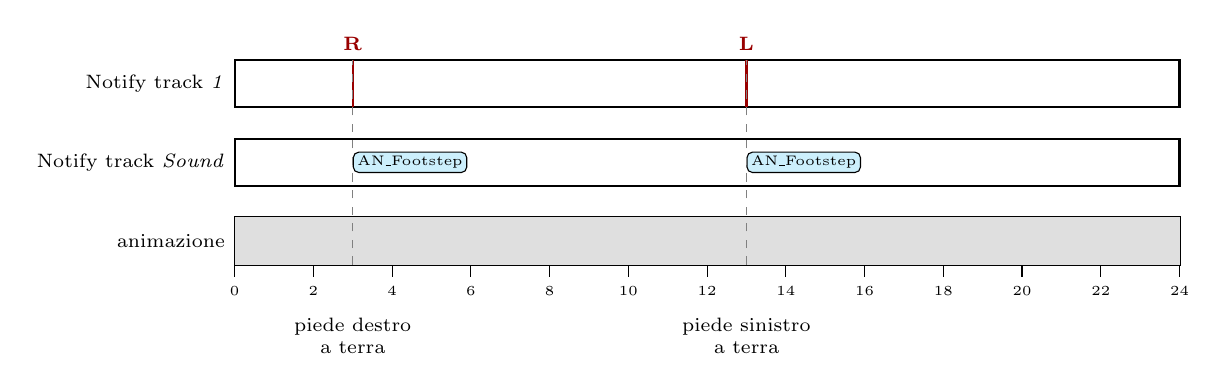
\begin{tikzpicture}[font=\footnotesize, x=0.5cm]
  \draw[thick] (0,0) rectangle (24,0.6);
  \node[left, font=\scriptsize] at (0,0.3) {Notify track \emph{1}};
  \draw[thick] (0,-1.0) rectangle (24,-0.4);
  \node[left, font=\scriptsize] at (0,-0.7) {Notify track \emph{Sound}};
  \draw[thick] (0,-2.0) rectangle (24,-1.4);
  \node[left, font=\scriptsize] at (0,-1.7) {animazione};
  \foreach \f in {0,2,...,24} {\draw (\f,-2.0) -- (\f,-2.15);
    \node[below, font=\tiny] at (\f,-2.15) {\f};}
  \fill[gray!25] (0,-2.0) rectangle (24,-1.4);
  \foreach \f/\n in {3/R, 13/L} {
    \draw[red!60!black, thick] (\f,0) -- (\f,0.6);
    \node[red!60!black, font=\scriptsize\bfseries, above] at (\f,0.6) {\n};
    \node[draw, fill=cyan!20, rounded corners=2pt, font=\tiny, inner sep=1.5pt, anchor=west]
      at (\f,-0.7) {AN\_Footstep};
    \draw[dashed, gray] (\f,-2.0) -- (\f,0.6);
  }
  \node[font=\scriptsize, align=center] at (3,-2.9) {piede destro\\a terra};
  \node[font=\scriptsize, align=center] at (13,-2.9) {piede sinistro\\a terra};
\end{tikzpicture}
\caption{La linea del tempo della corsa del bot (e delle due corse inclinate). Sulla
traccia \emph{1} i Sync Marker R e L ai frame 3 e 13; su una nuova traccia \emph{Sound}
l'AN\_Footstep negli stessi due punti. La lunghezza della linea del tempo è indicativa:
il numero totale di frame dell'animazione non si sente nella trascrizione. Schema
ricostruito.}
\label{ue10:fig:track}
\end{figure}

\paragraph{Approfondimento: Sync Marker, Blend Space e Notify doppi.} I Sync Marker non
sono legati alle ossa, come la trascrizione può far pensare, ma alla linea del tempo:
sono etichette con un nome (qui R e L) che segnano le fasi del passo. Servono quando
Unreal deve mescolare animazioni di durata diversa, nei Blend Space o con i
\emph{Sync Group}: invece di allinearle per tempo normalizzato, le allinea per marker, in
modo che i piedi tocchino terra insieme in tutte le animazioni mescolate. Funziona solo se
tutte le animazioni hanno gli stessi marker, con gli stessi nomi: è il motivo pratico per
cui il docente li aggiunge a tutte e tre le corse. I Notify, invece, pongono una domanda
diversa: in un Blend Space che sta mescolando tre animazioni, \emph{di quale} animazione
devono scattare i Notify? Nei Details del Blend Space, nella sezione \emph{Animation
Notifies}, l'opzione \emph{Notify Trigger Mode} decide: \emph{All Animations} (tutte quelle
che hanno un peso, con il rischio di sentire due o tre passi sovrapposti),
\emph{Highest Weighted Animation} (solo quella che pesa di più, la scelta più sicura per i
passi) o \emph{None}. Da notare infine che, nella lezione, la camminata a 250 non riceve
il Notify: a velocità intermedie i passi si sentono solo se il campione dominante è una
delle corse; per un risultato completo va aggiunto anche alla camminata, ai suoi frame di
appoggio. L'editor delle animazioni offre anche un Notify già pronto,
\emph{Play Sound}, che suona un suono senza Blueprint (il suo limite è che non sa
distinguere le superfici), e i \emph{Notify State}, che hanno un inizio e una fine invece
di un istante.

% ---------------------------------------------------------------------
\section{I Physical Material e le pedane}
\label{ue10:sec:physmat}

``Adesso, se noi andiamo in play, andiamo a vedere. Guardate un po'.'' A ogni passo
compare il trace che identifica il terreno, ``in questo caso il terreno di default''. ``Ma
come facciamo a dire, guarda, questo è un terreno diverso da quello normale? Dobbiamo
usare i Physics Material.''

\paragraph{Creare i Physical Material.} Una cartella \textbf{PhysicsMaterial} (``eccola
qua''); dentro, tasto destro, \textbf{Physics} $\rightarrow$ \textbf{Physical Material}. Se
ne creano due: \textbf{PM\_Rock} e \textbf{PM\_Water}. Poi, ``una cosa molto semplice,
ragazzi'': doppio clic su ciascuno; c'è la proprietà \textbf{Surface Type}, che di default
vale \emph{Default}: per PM\_Water si sceglie \textbf{Water}, per PM\_Rock \textbf{Rock}.
I nomi sono quelli scritti nelle Project Settings (figura~\ref{ue10:fig:catena}).

\paragraph{Le pedane.} ``L'unica cosa che ci manca è prendere una qualsiasi superficie.'' Un
blocco del livello, clonato (\textbf{Alt} più trascinamento, o duplicato) e schiacciato:
``fate un pianerottolino piccoletto'', due pedane. ``Adesso non abbiamo i materiali, ad
esempio, dell'acqua e della terra, ma ne mettiamo due a caso'': un materiale \emph{solid
blu} per l'acqua, \emph{Boulder} per la roccia; sono solo un segnale visivo. Poi:
selezionata la Static Mesh, ``andiamo giù, giù, giù, fino a trovare il \textbf{Phys
Material Override}'', e lì \textbf{PM\_Water} per l'acqua, \textbf{PM\_Rock} per la
roccia. ``Adesso, se noi andiamo sopra con il character, sentiamo che'' sulla roccia il
passo cambia. ``Eccolo qua.''

\begin{figure}[htbp]
\centering
\begin{tikzpicture}[font=\footnotesize,
  ue10box/.style={draw, thick, rounded corners=4pt, align=center, fill=gray!8,
                 minimum height=1.1cm, text width=2.5cm},
  ue10arr/.style={-{Stealth[length=2.5mm]}, thick}]
  \node[ue10box, fill=blue!8] (ps) at (0,0) {\textbf{Project Settings}\\{\scriptsize
    Engine, Physics, Physical Surface: Rock, Water}};
  \node[ue10box, fill=orange!12] (pm) at (4.3,0) {\textbf{PM\_Rock}, \textbf{PM\_Water}\\
    {\scriptsize Physical Material, Surface Type}};
  \node[ue10box, fill=green!10] (sm) at (8.6,0) {\textbf{Pedana}\\{\scriptsize Static
    Mesh, Phys Material Override}};
  \node[ue10box, fill=yellow!15] (tr) at (12.9,0) {\textbf{AN\_Footstep}\\{\scriptsize
    trace, Hit Result, Get Surface Type, Switch}};
  \node[ue10box, fill=violet!12] (cue) at (12.9,-2.4) {\textbf{Sound Cue}\\{\scriptsize
    Footstep, Rock, Water}};
  \node[ue10box, fill=red!10] (an) at (8.6,-2.4) {\textbf{Animazioni di corsa}\\
    {\scriptsize Notify ai frame 3 e 13}};
  \draw[ue10arr] (ps) -- node[above, font=\scriptsize]{nomi} (pm);
  \draw[ue10arr] (pm) -- node[above, font=\scriptsize]{assegnato} (sm);
  \draw[ue10arr] (sm) -- node[above, font=\scriptsize]{colpita} (tr);
  \draw[ue10arr] (tr) -- node[right, font=\scriptsize]{sceglie} (cue);
  \draw[ue10arr] (an.north east) -- node[below right, font=\scriptsize, pos=0.4]{fa
    scattare} (tr.south west);
\end{tikzpicture}
\caption{La catena completa dei passi. I nomi delle superfici nascono nelle Project
Settings, vengono assegnati ai Physical Material, che a loro volta si assegnano alle
superfici del livello; a ogni passo, il Notify inserito nell'animazione lancia il trace,
legge la superficie colpita e sceglie il Sound Cue. Schema ricostruito.}
\label{ue10:fig:catena}
\end{figure}

\paragraph{La spiegazione ripetuta.} A uno studente che chiede dove trovare ``i cosini''
(i PM): ``quelli li crei, praticamente. Lo fai con tasto destro, Physics, Physical
Material, e lo crei. Lo chiami PM\_Rock, come vuoi, PM\_Rock e PM\_Water. Ci clicchi su
ognuno di essi e gli cambi il Surface Type: lo metti Rock per il rock e Water per il
water. Poi, fatto questo, prendi un qualsiasi asset (vabbè, anche un blocco va
benissimo): devi andare su Phys Material Override e gli metti il Physical Material.''
``Basta che fai due pedanine'': ``qualsiasi superficie che tu vuoi prendere, ci puoi
camminare sopra''; ``la scali, fai quello che vuoi, fondamentalmente''.

\paragraph{Approfondimento: dove si assegna un Physical Material.} Il \emph{Phys Material
Override} usato a lezione vale per tutto il componente: comodo per una pedana, poco
pratico per un terreno che cambia da un punto all'altro. Unreal offre altri due posti. Il
primo è il \textbf{materiale}: nei Details di un Material (o di un Material Instance) c'è
la proprietà \emph{Phys Material}; tutte le mesh che usano quel materiale ``diventano''
roccia o acqua, senza toccare il livello, ed è la soluzione abituale nei progetti veri.
Il secondo è il \textbf{Landscape}: ogni layer dipinto può avere il suo Physical Material,
e il trace legge quello del layer dominante nel punto colpito. In più, il Physical
Material non serve solo ai suoni: contiene l'attrito (\emph{Friction}), il rimbalzo
(\emph{Restitution}) e la densità usati dalla simulazione fisica, ed è la base per gli
effetti d'impatto dei proiettili (scintille sul metallo, polvere sulla pietra), con la
stessa tecnica del Get Surface Type e dello Switch.

% ---------------------------------------------------------------------
\section{Gli ultimi problemi e la chiusura}
\label{ue10:sec:chiusura}

\paragraph{Gli ultimi problemi.} ``Un attimo: è successo un casino? Gli altri? Qualche
problema? Funziona?''
\begin{itemize}
  \item Uno studente si è perso il primo pezzo del grafo dell'AN\_Footstep e non sa da
        dove vengano Mesh Comp, Animation ed Event Reference: sono gli ingressi di
        Received\_Notify, la funzione sovrascritta con \emph{Override}. Poi, di nuovo, la
        catena: ``Get Owner, Get Actor Location, Get Actor Up Vector, e poi sottrai,
        per far sì che'' End sia sotto lo Start, ``che è il Get Actor Location''.
  \item Lo stesso studente ha messo le pedane, ma il personaggio non fa nessun rumore,
        nemmeno sul pavimento normale. I suoni nell'Anim Notify ci sono (``Rock1, Water
        Cue, Footstep Cue: va benissimo''); l'errore è nel vettore: il Get Actor Up Vector
        era collegato al pin sbagliato del Multiply. ``Mettilo sopra; stacca quello
        sotto; tasto destro su quello là, to float, 250.'' Con il Draw Debug Type a For
        Duration e una ricompilazione, il passo si sente.
  \item Le pedane, però, non fanno il suono della roccia: ``fammi vedere se hai messo la
        cosa'', e infatti il Phys Material Override non c'era. Lo studente non riesce a
        scendere nei Details fino alla voce: il pannello era filtrato su una categoria
        (\emph{Generale}); cliccando su \emph{Tutto} e aprendo la parte avanzata della
        sezione \emph{Physics} (``vai su tutto, clicca su tutto; giù, eccolo là''), si
        trova \emph{Phys Material Override}. ``A posto, perfetto.''
  \item ``A me non compaiono le linee'': ``basta che fai Draw Debug Type e la metti For
        Duration'', sul Line Trace By Channel. ``Quello è solo una cosa di debug,
        tranquilli.''
\end{itemize}

\paragraph{L'inclinazione rimandata.} ``Io ho sempre quella cosa dell'inclinazione della
testa'': è la studentessa del Lean che non inclina. ``Possiamo farlo la prossima volta?''
``Sì, facciamo la prossima volta. Tanto la prossima volta facciamo interazioni, e allora
ricordamelo tu, eh?'' ``Così fixiamo tutto''; ``lo guardo poi in futuro, lo guardo poi in
post anche''.

\paragraph{Il calendario.} ``Io vi ringrazio per l'attenzione, grazie'' anche a chi segue
in differita. ``Ci vediamo giovedì per la prossima lezione, che faremo in questo caso i
menu: andiamo a fare un po' di UI.'' (Il docente, poco prima, aveva parlato di
``interazioni'': dalla trascrizione non si capisce se la lezione di giovedì conterrà
entrambe le cose.) Uno studente pensava che oggi fosse giovedì; il calendario: ``abbiamo
questo martedì, giovedì e, se non sbaglio, il 30, che è martedì prossimo: è l'ultima con
me. Poi ci avete Davide.'' ``Va bene, ragazzi. Allora ci vediamo. Buona cena. Buona
serata.''

\begin{table}[htbp]
\centering
\small
\begin{tabular}{@{}p{5.4cm}p{8.6cm}@{}}
\toprule
\textbf{Sintomo} & \textbf{Causa e rimedio} \\
\midrule
Il personaggio non si muove, errori su IA\_Run & IA\_Move cancellata e sostituita da
IA\_Run: duplicare IA\_Look (Vector 2D), rinominarla IA\_Move, rimetterla in IMC\_Default
e nell'evento \\
L'evento del movimento non mostra il vettore & salvare l'Input Action; poi Split Struct
Pin sull'Action Value \\
Dopo una compilazione ``sparisce tutto'' & il Blueprint non compila: leggere i Compiler
Results \\
Camera storta, movimento strano & Spring Arm attaccato alla freccia o spostato dal pivot:
riattaccarlo, location a zero, usare Target Arm Length, Socket Offset, Target Offset \\
La camera non segue il mouse & Use Pawn Control Rotation sullo Spring Arm \\
La torretta ignora il nuovo personaggio & manca il tag Player; controllare le risposte
ai trace e alle collisioni \\
Il Montage non si vede & manca lo Slot DefaultSlot nell'AnimGraph \\
Durante il Montage il corpo gira & il DefaultSlot prende tutte le ossa: serve uno slot
per la parte alta (Layered blend per bone) \\
Errori nell'Event Graph incollato & variabili del vecchio ABP: ricrearle con Create
variable, rifare le referenze nell'Initialize \\
\emph{Idle to Walk will never be taken} & la regola della transizione non è ancora
scritta \\
Lo stato non mostra l'anteprima del Blend Space & lo stato non è mai raggiunto
(transizione o dati mancanti) \\
Il personaggio levita & Mesh a Z = $-90$ \\
Il personaggio si muove in T-pose & State Machine non collegata all'Output Pose, o
Mesh senza Anim Class \\
Errori su Jump e Fall & regole vuote: Automatic Rule Based on Sequence Player in State, e
la regola Fall $\rightarrow$ Land Run \\
GroundSpeed sempre zero & due variabili Character Movement (una mai valorizzata), o
Update non collegato al Validated Get \\
Il Lean non inclina & segno e scala del Delta Rotator, opzioni di rotazione; rimandato
alla lezione successiva \\
La camera inclinata di lato & ruotata sulla X (Roll) invece che sulla Y (Pitch) \\
AN\_Footstep non compare in Add Notify & la classe ha un altro nome: cercarla con quello
\\
Nessun suono di passi & Up Vector sul pin sbagliato del Multiply; Notify non inserito
nelle animazioni \\
Le pedane suonano come il pavimento & manca il Phys Material Override, o il Surface Type
del Physical Material \\
Phys Material Override introvabile & filtro dei Details su Generale: scegliere Tutto e
aprire le opzioni avanzate \\
Le linee del trace non si vedono & Draw Debug Type a For Duration \\
\bottomrule
\end{tabular}
\caption{I problemi incontrati durante la lezione, con la causa e il rimedio.}
\label{ue10:tab:errori}
\end{table}

\begin{table}[htbp]
\centering
\small
\begin{tabular}{@{}p{4.8cm}p{9.2cm}@{}}
\toprule
\textbf{Nodo, asset o impostazione} & \textbf{Che cosa fa} \\
\midrule
Input Action, Value Type Vector 2D & azione con un valore a due assi (movimento,
sguardo) \\
Add Movement Input & muove il Pawn lungo una direzione, con una scala \\
Tags (Actor) & etichette con cui altri Blueprint riconoscono l'actor \\
Try Get Pawn Owner / Cast To & il Pawn che possiede l'animazione; la sua classe precisa \\
Promote to Variable & salva un'uscita in una nuova variabile \\
Convert to Validated Get & Get con controllo di validità (Is Valid / Is Not Valid) \\
Create variable (tasto destro) & crea la variabile mancante di un nodo incollato \\
Comment (tasto C) / Reroute Node (doppio clic sul filo) & riquadro con titolo; punto di
piegatura di un filo \\
Blend Space 2D: Lean e GroundSpeed & mescola le corse inclinate e la camminata \\
Get Owning Actor / Get Actor Rotation & l'actor proprietario; la sua rotazione \\
Delta Rotator & la differenza normalizzata fra due rotazioni \\
FInterp To / RInterp To & un passo d'interpolazione fra float; fra rotator \\
Get World Delta Seconds & il tempo dell'ultimo frame \\
State Machine, Can Enter Transition & stati e regole booleane di passaggio \\
Automatic Rule Based on Sequence Player in State & la transizione scatta a fine
animazione \\
AND Boolean / NOT Boolean & congiunzione; negazione \\
Get Last Input Vector & l'ultimo input di movimento del Pawn (lunghezza 0--1) \\
Vector Length & la lunghezza di un vettore \\
Print String & scrive un valore a schermo, per il debug \\
World Settings: Default Pawn Class & il personaggio del giocatore nel livello \\
Anim Notify (classe), Received\_Notify & evento in un istante dell'animazione; la funzione
che lo riceve \\
Get Owner / Get Actor Location / Get Actor Up Vector & proprietario; posizione; vettore
verso l'alto \\
Line Trace By Channel, Draw Debug Type & trace lungo un segmento; disegno di debug \\
Break Hit Result: Impact Point & il punto esatto dell'impatto \\
Get Surface Type & il tipo di superficie colpita (dal Physical Material) \\
Physical Surface (Project Settings) & i nomi dei tipi di superficie \\
Switch on EPhysicalSurface & un'uscita per ogni tipo di superficie \\
Play Sound at Location & suona un suono in un punto \\
Sound Wave / Sound Cue & file audio; grafo che combina e modula i suoni \\
Create Single Cue & crea un Cue dai Sound Wave selezionati (con Random) \\
Random / Modulator & sceglie un ingresso a caso; varia pitch e volume \\
Add Sync Marker & marcatore con nome sulla linea del tempo (R, L) \\
Insert Notify Track / Add Notify & nuova traccia di Notify; inserisce un Notify \\
Physical Material: Surface Type & il tipo di superficie dell'asset \\
Phys Material Override & assegna un Physical Material a un componente \\
\bottomrule
\end{tabular}
\caption{I nodi, gli asset e le impostazioni della decima lezione.}
\label{ue10:tab:nodi}
\end{table}

% ---------------------------------------------------------------------
\section*{Punti chiave del capitolo}
\addcontentsline{toc}{section}{Punti chiave del capitolo}

\begin{itemize}
  \item Un'\textbf{Input Action} cancellata rompe il personaggio in modo silenzioso: si
        ricrea duplicando un'azione dello stesso tipo (\textbf{IA\_Look}, Vector 2D, per
        \textbf{IA\_Move}), la si rimette nell'\textbf{IMC} e nell'evento. Lo
        \textbf{Spring Arm} non si sposta dal pivot: si regolano Target Arm Length,
        Socket Offset e Target Offset.
  \item Quando si cambia personaggio, tutto ciò che riconosceva il vecchio va
        ricontrollato: \textbf{tag} (Player per la torretta), \textbf{cast} a classi
        precise, \textbf{collisioni} e risposte ai trace.
  \item Un Animation Blueprint si può costruire \textbf{copiando} l'Update di un altro, ma
        l'\textbf{Initialize} si rifà: Try Get Pawn Owner, Cast To, referenze promosse a
        variabile, ``un gancio'' fra animazione e personaggio. Le variabili mancanti si
        ricreano con \textbf{Create variable}; il \textbf{Validated Get} protegge l'Update.
        Attenzione alle variabili doppie (Character Movement 0).
  \item Ordine nel grafo: \textbf{commenti} con il tasto C, \textbf{Reroute} con un doppio
        clic sul filo.
  \item Il \textbf{Blend Space 2D} del bot ha il \textbf{Lean} in orizzontale ($-10$,
        10) e la \textbf{GroundSpeed} in verticale (0--500, la Max Walk Speed): corsa e
        corse inclinate a 500, camminata a 250, nessun Idle.
  \item Il \textbf{Lean} si calcola a ogni frame: rotazione attuale, \textbf{Delta
        Rotator} con quella precedente, lo \textbf{Yaw}, \textbf{FInterp To} verso quel
        valore (Interp Speed 1--5, Get World Delta Seconds), poi la rotazione attuale
        diventa la precedente. Segno e scala vanno verificati.
  \item La \textbf{State Machine} ha sette stati: Idle e Walk (GroundSpeed $>$ 0, $\le$
        0), Jump Idle e Jump Run (IsFalling AND la velocità), Fall (automatica dopo i
        salti), Land Idle e Land Run (NOT IsFalling AND [NOT] \textbf{ReceiveInput}),
        ritorni automatici. ReceiveInput viene da \textbf{Get Last Input Vector}: la
        lunghezza maggiore di zero dice che il giocatore sta premendo.
  \item Per giocare con il bot: Spring Arm e Camera a zero, Target Offset, \textbf{Default
        Pawn Class} nelle World Settings, i grafi di input copiati dal vecchio
        personaggio, Use Pawn Control Rotation, Mesh a $-90$.
  \item I passi: un \textbf{Anim Notify} (AN\_Footstep, \textbf{Received\_Notify}) lancia
        un \textbf{Line Trace By Channel} di 250 centimetri verso il basso; dal Hit Result,
        \textbf{Get Surface Type} e \textbf{Switch on EPhysicalSurface} scelgono il
        \textbf{Play Sound at Location} sull'\textbf{Impact Point}.
  \item I tipi di superficie si definiscono nelle \textbf{Project Settings} (Physics,
        Physical Surface: Rock, Water); i \textbf{Physical Material} (PM\_Rock, PM\_Water)
        li assegnano con il Surface Type; il \textbf{Phys Material Override} li applica
        alle mesh del livello.
  \item I \textbf{Sound Cue} variano i passi: \textbf{Random} fra più Sound Wave
        (\emph{Create Single Cue}) e \textbf{Modulator} sul pitch (passo 0,95--1,3, roccia
        2--2,2, acqua 1,3--1,5).
  \item Nelle animazioni di corsa: \textbf{Sync Marker} R e L e una \textbf{Notify Track}
        \emph{Sound} con l'AN\_Footstep ai frame di appoggio (3 e 13), in tutte e tre le
        animazioni.
\end{itemize}

%
%  Tutte le etichette di questo capitolo hanno il prefisso "ue10:"
%  (ue10:cap:..., ue10:sec:..., ue10:fig:..., ue10:tab:...), e tutti gli
%  stili TikZ hanno il prefisso "ue10" (ue10node, ue10exec, ue10data,
%  ...) per non collidere con chiavi native di TikZ né con quelli delle
%  lezioni precedenti. Il capitolo è autonomo: non contiene \ref verso
%  altri capitoli (i rimandi alle lezioni precedenti sono a parole).
%  Le figure sono ricostruzioni schematiche di quanto mostrato e detto a
%  lezione, non copie delle schermate del docente. Dove la trascrizione
%  è troppo rovinata per ricostruire un dettaglio, il capitolo lo dice
%  invece di inventarlo.
% =====================================================================

\chapter[Lean, State Machine e Physical Material]{Il nuovo personaggio: Lean,
State Machine e passi con i Physical Material}
\label{ue10:cap:bot}

Questa è la \textbf{decima lezione} del corso breve di \textbf{introduzione a Unreal
Engine}. Alla fine della nona il docente aveva lasciato un compito facoltativo: costruire
da zero un personaggio nuovo con lo \textbf{StackOBot}, il robottino dei progetti di
esempio di Epic, che ha già tutte le sue animazioni. Il compito era ``molto facoltativo,
perché capisco che è complicato''; in questa lezione lo si fa insieme, dall'inizio alla
fine: ``faremo proprio un nuovo character, che useremo poi come default''.

Il nuovo personaggio riprende la struttura del cavaliere della lezione precedente
(Animation Blueprint, State Machine, Blend Space), ma con tre differenze che danno il
titolo al capitolo. La prima è il \textbf{Lean}: il bot non ha otto animazioni
direzionali, ma una corsa e due varianti \emph{inclinate}, verso sinistra e verso
destra; il Blend Space 2D non usa più la direzione, ma un valore d'inclinazione calcolato
a ogni frame dalla differenza fra la rotazione attuale e quella del frame precedente. La
seconda è una \textbf{State Machine} più ricca, a sette stati, che distingue il salto da
fermo dal salto in corsa e l'atterraggio da fermo dall'atterraggio in movimento, con una
nuova variabile che dice se il giocatore sta premendo un tasto di movimento. La terza è
il suono dei \textbf{passi}: un \textbf{Anim Notify} inserito nelle animazioni, nel
momento esatto in cui il piede tocca terra, lancia un \emph{line trace} verso il basso,
legge il tipo di superficie colpita e suona il passo giusto; le superfici si distinguono
con i \textbf{Physical Material}, ``i materiali che possono determinare uno stato fisico''
di un oggetto. Sulla roccia si sente la roccia, sull'acqua l'acqua, altrove il passo
normale.

La lezione è \textbf{online}, su Zoom, come le precedenti. Si apre con una lunga
correzione in diretta del progetto di uno studente, prosegue con la costruzione del bot,
interrotta più volte dalle domande e dai problemi dei presenti, risolti in condivisione di
schermo, e si chiude sui passi e i Physical Material. La pausa arriva dopo la variabile
dell'input (``ci vediamo alle solite 18. Scusate: 17.55''); alla fine, ``vi mando a
cena''. È una lezione di \emph{fine corso}: ``mancano tre lezioni alla fine'', e il
docente lo ricorda per invitare chi segue in differita a entrare in diretta, se vuole
correzioni dal vivo.

Tre avvertenze di lettura, le stesse delle lezioni precedenti. La prima: la trascrizione
è automatica e storpia moltissimi nomi. Unreal è ``Arreal'', ``ArRIAL'', ``a Real'' e
``Arriva''; il \textbf{Lean} è ``Lin'', ``Line'', ``l'in'', ``LIN'' e ``Linn'' (``l'in è il
piegamento della rotazione''); l'\textbf{Idle} è ``idol'' e ``Idol''; l'\textbf{Event
Graph} è ``even graph'', ``Even Graph'' e ``Vengraph''; l'\textbf{AnimGraph} è
``Alimgraph'', ``aningraf'' e ``Aningraft''; \textbf{IA\_Move} è ``IAMove'', ``iam
move'', ``Iammov'' e ``gli ammove''; \textbf{IA\_Run} è ``iaran'', ``IRRun'' e ``iarran'';
l'\textbf{IMC} è ``IAMC'' e ``negli MC''; il \textbf{Then 0} della Sequence è
``DANZIRO'' e ``den zero''; i \textbf{Reroute Node} sono ``re Routenold''; il
\textbf{Blend Space} è ``Benzes'' e ``Brennese''; il \textbf{Validated Get} è ``validate
get''; l'\textbf{FInterp To} è ``F inter2'' e ``fintech 2''; l'\textbf{RInterp To} è ``R
inter to''; l'\textbf{Is Falling} è ``his falling'' e ``ease falling''; il \textbf{Last
Input Vector} è ``Lasting Pwn Vector''; lo \textbf{Spring Arm} è ``Springarma'' e
``spring guard''; \textbf{Use Pawn Control Rotation} è ``PoundCtrlRotation'', ``Pwn
rotation'' e ``use spawn control rotation''; le \textbf{World Settings} sono ``Word
Settings'' e la \textbf{Default Pawn Class} è ``default on class''; l'\textbf{Anim
Notify} è ``an in notify'', ``Anim Notifaj'', ``modify'', ``anni nota'' e ``anni
notifà''; \textbf{AN\_Footstep} è ``a n footstep'' e ``AN full step''; il
\textbf{Physical Material} è ``fisic material'' e ``P FIS materia''; \textbf{Get Surface
Type} è ``Gethsurfest Type'' e ``get sur festival''; il \textbf{Sound Cue} è ``queue'' e
``Q''; il \textbf{Draw Debug Type} è ``drop the bug type'' e ``draw the bug type''; il
\textbf{Break Hit Result} è ``break it risult''; \textbf{BP\_Knight} è ``BP Night'' e
``Night''; il \textbf{bot} è a tratti ``Boto'' e ``voto''. Dove la ricostruzione è
sicura il capitolo usa la forma corretta; dove non lo è riporta la forma della
trascrizione e lo dice. La seconda: all'inizio della registrazione e durante la pausa il
riconoscimento vocale produce lunghi blocchi di testo senza senso e ripetuto (``grazie a
tutti per l'attenzione che ci ha spiegato'', ``qual è la risposta che ci può essere?'',
``la situazione è questa, la migliore dal 2005'', il ``rinforzare la democrazia'', la
``dottrina sul mercato del lavoro'', il ``dialogo interculturale''): non appartengono
alla lezione e sono stati ignorati. La terza: buona parte della lezione è fatta di
indicazioni a voce mentre si lavora (``vai su'', ``clicca qua'', ``attacca quello
sotto''), spesso rivolte allo schermo di uno studente; il capitolo ricostruisce i grafi
da ciò che il docente dice mentre li costruisce, distingue i tentativi dalle soluzioni,
completa i nomi esatti dei nodi e dei pin di Unreal Engine 5, e dichiara i punti in cui
la trascrizione lascia un buco.

\paragraph{Come leggere questo capitolo.} Il capitolo segue l'ordine della lezione. Le
figure ricostruiscono il movimento riparato con l'Enhanced Input, i due eventi
dell'Animation Blueprint del bot con il Validated Get, il calcolo del Lean, il Blend
Space 2D del bot, la State Machine a sette stati, il grafo dell'Anim Notify dei passi, la
catena che porta dalla superficie al suono, il Sound Cue con Random e Modulator, e la
linea del tempo dell'animazione di corsa con i Sync Marker e i Notify. Le tabelle
riassumono le transizioni della State Machine, i valori dei Sound Cue, gli errori
incontrati durante la lezione e i nodi della giornata. Qua e là, dei paragrafi di
\textbf{approfondimento} collegano la lezione ai libri di Marcos Romero e Brenden Sewell
(\emph{Blueprints Visual Scripting for Unreal Engine 5} e la seconda edizione dello
stesso testo, scritta per Unreal Engine 4), i testi di riferimento per questa parte del
libro, e a qualche nozione tecnica generale su Unreal Engine 5; sono segnalati come tali
e non fanno parte della lezione.

Il percorso del capitolo:
\begin{enumerate}
  \item l'\textbf{inizio della lezione}: il movimento e la camera riparati in diretta
        (sezione~\ref{ue10:sec:riparazione});
  \item gli \textbf{annunci} e le domande: i passi e i Physical Material, il compito
        facoltativo, il personaggio nuovo che non interagisce con il livello, la lezione
        di giovedì, il bot di Federico (sezioni \ref{ue10:sec:annunci}
        e~\ref{ue10:sec:federico});
  \item il \textbf{risultato finale}, mostrato in anteprima
        (sezione~\ref{ue10:sec:demo});
  \item il nuovo personaggio: \textbf{Animation Blueprint} e \textbf{Blueprint
        Character}, l'Event Graph copiato, l'\textbf{Initialize} e il \textbf{Validated
        Get}, commenti e Reroute (sezioni da~\ref{ue10:sec:abp}
        a~\ref{ue10:sec:commenti});
  \item il \textbf{Blend Space 2D} del bot e il calcolo del \textbf{Lean} (sezioni
        \ref{ue10:sec:blend} e~\ref{ue10:sec:lean});
  \item la \textbf{State Machine} a sette stati, la variabile dell'\textbf{input} e le
        regole di transizione, prima e dopo la pausa (sezioni da~\ref{ue10:sec:sm}
        a~\ref{ue10:sec:transizioni2});
  \item il bot \textbf{in gioco}, con la camera, e il debug dei progetti degli studenti
        (sezioni \ref{ue10:sec:ingioco} e~\ref{ue10:sec:debug});
  \item i \textbf{passi}: l'\textbf{Anim Notify}, il \emph{line trace}, i
        \textbf{Physical Surface}, i \textbf{Sound Cue}, i \textbf{Notify} nelle
        animazioni e i \textbf{Physical Material} (sezioni da~\ref{ue10:sec:notify}
        a~\ref{ue10:sec:physmat});
  \item gli ultimi problemi e la \textbf{chiusura}
        (sezione~\ref{ue10:sec:chiusura}).
\end{enumerate}

% ---------------------------------------------------------------------
\section{Prima della lezione: il movimento da riparare}
\label{ue10:sec:riparazione}

Dopo i minuti iniziali di rumore della trascrizione, i saluti (``buongiorno, buon
pomeriggio'') e una prima richiesta. Mentre gli altri ``stanno ancora entrando'', uno
studente racconta il suo problema: ha seguito la lezione precedente in differita (``ho
seguito la lezione da quando è stata salvata''), e all'inizio ``andava tutto, si
muoveva''; poi, a un certo punto, il personaggio non si muoveva più, e ``la camera,
anche se segnata, non c'è, ed è sparito tutto''. Il docente propone di risolverlo subito
(``tanto adesso stanno ancora entrando'') e la correzione si fa in condivisione di
schermo. È una sequenza lunga e caotica, ma istruttiva: mostra come si legge un errore di
compilazione e come si ricostruisce un pezzo di Enhanced Input perduto.

\paragraph{Leggere gli errori.} ``Già ti dico che comunque possiamo già vedere gli
errori là sotto'': il pannello dei risultati della compilazione (\emph{Compiler
Results}) in fondo all'editor del Blueprint elenca i nodi che non trovano più ciò a cui
si riferiscono. La prima diagnosi, a colpo d'occhio: ``sicuramente ti manca
l'\emph{Input Action}''. L'errore dice che l'evento di \textbf{IA\_Run} non esiste più
nel nodo, o che il contesto \textbf{IMC\_Default} non lo contiene: ``dice che
fondamentalmente non hai IA\_Run: l'hai cancellato per sbaglio oppure non l'hai mai
creato?''. In realtà IA\_Run c'è (``il Content Browser, fai IA\_Run, ed eccolo là''): il
problema è un altro.

\paragraph{IA\_Move cancellata.} Aprendo l'\textbf{IMC\_Default} (``scrivi IMC, invece di
IAMC''), il docente trova dei mapping che lo studente non ricorda di aver messo (``ma no,
non li ho messi io''): li si cancella tutti con il cestino, poi si torna indietro con
\textbf{Ctrl+Z} (``fai Ctrl+Z a tutti, va benissimo''). Guardando il mapping che dovrebbe
essere \textbf{IA\_Move} si capisce: ``hai cancellato IA\_Move, fondamentalmente'', e al
suo posto, nell'Event Graph, l'evento del movimento è stato sostituito da IA\_Run (``ah,
perché l'hai sostituito''). ``E devi stare attento a queste cose.''

\paragraph{Ricreare IA\_Move.} ``La cosa che devi fare adesso è praticamente ricreare
IA\_Move.'' Il primo istinto è duplicare IA\_Run; poi il docente si corregge: ``no, no,
no: fai un doppione di \textbf{IA\_Look}''. Il motivo è il tipo di valore: IA\_Run è un
booleano (\emph{Digital}), mentre il movimento, come lo sguardo, è un \textbf{Vector 2D}
(``è un Vector 2D''): duplicare IA\_Look dà un'azione già del tipo giusto. Il doppione si
rinomina \textbf{IA\_Move}. Poi, nell'IMC\_Default:
\begin{itemize}
  \item si rimette IA\_Move nel mapping che lo usava prima (``adesso segnali negli MC
        quello di prima, IA\_Move'');
  \item con il \textbf{più} in alto si crea un altro mapping, per \textbf{IA\_Run}: con la
        freccina sotto il nome si apre la scelta del tasto e, invece di cercarlo nella
        lista, ``basta che clicchi sulla tastiera: clicca Shift sulla tua tastiera''. Il
        campo del tasto, quando è in ascolto, registra il primo tasto premuto.
\end{itemize}
Una compilazione di prova: ``qualche cosa si è levato, benissimo''.

\paragraph{L'evento e gli Add Movement Input.} Restano gli errori nell'Event Graph del
personaggio (il cavaliere, ``Knight''): ``hai sostituito IA\_Move con IA\_Run: devi levare
questo e mettere IA\_Move''; con il tasto destro si ricrea l'evento \textbf{IA\_Move}.
Uno strano dettaglio (``strano che non ti fa vedere'') si risolve salvando l'azione: solo
dopo il salvataggio l'evento mostra l'\textbf{Action Value} come vettore 2D. Si ricostruisce
il grafo del movimento, quello copiato la volta precedente dal ThirdPersonCharacter:
\begin{enumerate}
  \item tasto destro sull'\textbf{Action Value} e \textbf{Split Struct Pin}, per avere i
        pin \textbf{X} e \textbf{Y} separati;
  \item la \textbf{X} si collega al primo \textbf{Add Movement Input}, la \textbf{Y}
        ``tutto dritto fino a Scale Value del successivo'';
  \item il secondo Add Movement Input era stato cancellato (``ah, non c'è''): lo si
        ricopia dal primo (``copia Add Movement Input'');
  \item nella \textbf{World Direction} si collega ``quel forward vector che c'è lì
        vicino, quello arancione'' (il vettore di direzione calcolato dalla rotazione
        del controller);
  \item infine il pin di esecuzione: dal \textbf{Triggered} di IA\_Move, ``attacchi
        tutto in sequenza''.
\end{enumerate}
``E abbiamo riparato il movimento'' (figura~\ref{ue10:fig:move}). Compilato, il
personaggio si muove.

\begin{figure}[htbp]
\centering
\begin{tikzpicture}[font=\footnotesize,
  ue10node/.style={draw, thick, rounded corners=4pt, align=center, fill=gray!8,
                  minimum height=0.9cm, text width=3.4cm},
  ue10ev/.style={ue10node, fill=red!12},
  ue10exec/.style={-{Stealth[length=2.5mm]}, very thick, black!80},
  ue10data/.style={-{Stealth[length=2mm]}, thick, blue!60!black}]
  \node[ue10ev, text width=2.6cm, minimum height=2.0cm] (ev) at (0,0)
    {\textbf{IA\_Move}\\{\scriptsize Enhanced Input Action}\\{\scriptsize Action Value
    (Vector 2D), split in X e Y}};
  \node[ue10node] (a1) at (5.0,0.9) {\textbf{Add Movement Input}\\
    {\scriptsize World Direction: vettore destro; Scale Value: X}};
  \node[ue10node] (a2) at (10.0,0.9) {\textbf{Add Movement Input}\\
    {\scriptsize World Direction: vettore avanti; Scale Value: Y}};
  \node[ue10node, fill=green!10, text width=4.2cm] (rot) at (7.5,-1.9) {Get Control
    Rotation (solo lo Yaw) $\rightarrow$ vettori \textbf{Forward} e \textbf{Right}};
  \draw[ue10exec] (ev.east |- a1) -- node[above, font=\scriptsize]{Triggered} (a1);
  \draw[ue10exec] (a1) -- (a2);
  \draw[ue10data] (rot.west) -| node[pos=0.75, left, font=\scriptsize]{Right}
    (a1.south);
  \draw[ue10data] (rot.east) -| node[pos=0.75, right, font=\scriptsize]{Forward}
    (a2.south);
  \draw[ue10data, dashed] (ev.south) |- node[pos=0.75, below, font=\scriptsize]{X
    $\rightarrow$ Scale Value del primo, Y $\rightarrow$ Scale Value del secondo}
    (rot.south west);
\end{tikzpicture}
\caption{Il movimento riparato. L'Action Value di IA\_Move, un Vector 2D, viene diviso in
X e Y: la X muove lungo il vettore destro, la Y lungo quello in avanti, entrambi ricavati
dalla rotazione del controller. Se IA\_Move viene cancellata o sostituita da un'azione
booleana (IA\_Run), l'Action Value non è più un vettore e il grafo si rompe. Schema
ricostruito dal grafo standard del ThirdPersonCharacter; l'ordine esatto delle due
direzioni a lezione non si sente.}
\label{ue10:fig:move}
\end{figure}

\paragraph{Perché ``sparisce tutto''.} Lo studente aveva notato che a volte il
personaggio compariva e a volte, dopo una compilazione, ``proprio scompariva tutto''.
``È normale'': quando la compilazione di un Blueprint fallisce, Unreal ``te lo fa capire
in modo molto più palese'': l'icona del pulsante \emph{Compile} diventa rossa, con un
simbolo d'errore (``un'iconcina''), e un Blueprint che non compila non si comporta come
dovrebbe in gioco.

\paragraph{La camera storta.} In Play il movimento funziona, ma ``è un po' strano'', e la
camera è ``molto storta''. Tre correzioni, nell'ordine:
\begin{enumerate}
  \item \textbf{Use Pawn Control Rotation}: selezionato lo \textbf{Spring Arm}, si cerca
        ``control rotation'' e si mette la spunta (``mettilo true, perfetto''): la
        telecamera segue il controller.
  \item \textbf{La gerarchia}: la camera era stata agganciata alla \emph{freccia}
        (l'\emph{Arrow Component} del Character): ``attenzione a fare queste cose''. Lo
        Spring Arm va staccato dalla freccia e attaccato al suo posto; la Camera ``deve
        rimanere'' figlia dello Spring Arm.
  \item \textbf{La posizione}: lo Spring Arm era stato spostato con il \emph{pivot}
        (``l'hai spostato sulla location''): ``devi mettere tutto a zero''. Accanto ai
        valori della Location, nei Details, c'è una freccina circolare tutta a destra che
        li riporta al default.
\end{enumerate}
La regola, ripetuta: lo Spring Arm e la Camera non si muovono dal pivot, ``perché se no
si rompe tutto''. Per spostare la camera si usano solo i valori dello Spring Arm:
\textbf{Target Arm Length}, \textbf{Socket Offset} e \textbf{Target Offset}. ``Se muovi
il pivot, ti cambia la location del braccio, quindi ti fa tutto un effetto strano anche
con la camera.'' Siccome lo studente voleva una visuale più alta: \textbf{Target Offset},
Z (``l'ultima a destra'') a \textbf{60}. ``E già la telecamera dovrebbe essersi fissata
più o meno'': ``abbastanza bene''.

\paragraph{Le animazioni del giorno prima.} Lo studente aveva fatto anche ``la roba delle
animazioni'' (``oddio, è un po' buggato''), ma senza poterla provare, perché il
personaggio era fermo. ``Tanto oggi la riprenderemo'': si rifarà un personaggio ``proprio
da capo''.

% ---------------------------------------------------------------------
\section{Gli annunci e le domande}
\label{ue10:sec:annunci}

\paragraph{La cartella Footstep Sounds.} ``Oggi andremo a vedere anche una cosettina
interessante.'' Il docente l'ha scritto su Discord: nella cartella del materiale
didattico, su Drive, c'è una cartella \textbf{Footstep Sounds}; va scaricata e
decompressa, ``lasciatela là'', servirà più tardi. Servirà per i \textbf{Physical
Material}, ``cioè praticamente i materiali che possono determinare uno stato fisico, ad
esempio di un oggetto'': ``se un oggetto è di metallo, come deve reagire in certi
ambiti''. Oggi li si usa per i passi: ``quando lui fa superficie acquosa si sentirà il
rumore dei passi dell'acqua, se no si sentirà il rumore dei passi della roccia, o si
sentirà il rumore dei passi normale: dipende dalla superficie in cui ci troviamo''.

\paragraph{Le correzioni in diretta.} ``Visto che tanto oggi andiamo diretti in
editor'': chi ha problemi con le lezioni passate e vuole ``delle correzioni un po' in
live, rispetto a che magari in post'', ha ancora ``questa lezione, la prossima e la
prossima ancora'': ``mancano tre lezioni alla fine''. L'invito vale anche per chi segue in
differita: ``entri, se vuole delle correzioni direttamente in live''.

\paragraph{Il compito sul bot.} Uno studente chiede se il bot andava fatto ``per oggi'',
``perché io non so neanche dove mettere le mani''. Il docente ripete che era un compito
``per i più coraggiosi'', ``molto facoltativo'', ``per chi magari gli piace smanettare'':
``tanto oggi lo faremo''. E, a scanso di equivoci: ``non vi metto un voto, state
tranquilli''.

\paragraph{Il personaggio nuovo che non interagisce.} Lo stesso studente ha due problemi
con il suo personaggio. Il primo: ``corre, ma non ha l'animazione della corsa''. ``La
prima probabilmente sarà un errore che andremo a vedere insieme.'' Il secondo è più
interessante: il personaggio nuovo ``non interagisce più con molte delle cose che
abbiamo fatto nelle lezioni passate''. Il bottone per chiamare l'ascensore funziona, ma
salire sull'ascensore no; l'ascensore ``quello col suono'' sì; la torretta no. Il
docente spiega il caso della torretta, ed è un principio generale: quando si cambia
personaggio, tutto ciò che nel livello riconosceva il vecchio personaggio va
ricontrollato.
\begin{itemize}
  \item \textbf{Il tag}: ``la torretta funziona tramite il tag, come gliel'abbiamo
        fatta''. Nelle lezioni precedenti la torretta cercava un actor con il tag
        \textbf{Player}: ``quindi, se cambiamo character, dobbiamo rimettergli il tag'',
        cioè aggiungere \emph{Player} ai \emph{Tags} del nuovo Blueprint. ``Guarda che
        questo è il player: segui lui.''
  \item \textbf{Le collisioni}: il nuovo personaggio deve rispondere ``ai trace che
        abbiamo fatto'' (la torretta \emph{vede} il giocatore con un trace) e alle
        collisioni ``che sono, ad esempio, la sfera'' (la sfera che fa scattare la
        torretta quando il giocatore entra nel suo raggio).
\end{itemize}
``Intanto lo faremo oggi'': ``faremo un nuovo character e andremo poi a risistemare un po'
tutto''.

\paragraph{La lezione di giovedì.} ``Piccola postilla'': i \textbf{menu}, che erano
rimasti ``un po' un buco aperto'', si faranno come lezione \textbf{opzionale}
\textbf{giovedì}; poi ci sarà ``un'ultima lezione finale con un'ultima cosa''. Ma ``se
volete proporre anche qualche argomento che vi interessa, fatelo un po' oggi'': se gli
studenti si mettono d'accordo, ``facciamo quello''; ``se no, andiamo con i menu
tranquillamente''.

\paragraph{Approfondimento: tag, collisioni e personaggi intercambiabili.} Il problema
dello studente è tipico di ogni progetto in cui il personaggio cambia. Le soluzioni
viste nelle lezioni precedenti riconoscono il giocatore in tre modi diversi, e ciascuno
si rompe in modo diverso: per \emph{tag} (\emph{Actor Has Tag}: basta aggiungere il tag
al nuovo Blueprint, nella sezione \emph{Actor} $\rightarrow$ \emph{Tags} dei Details);
per \emph{cast} a una classe precisa (un \emph{Cast To BP\_Knight} fallisce con qualunque
altro personaggio: è il motivo per cui conviene fare il cast alla classe più generale che
serve, \emph{Character} o \emph{Pawn}, o usare un'interfaccia); per \emph{collisione}
(il nuovo personaggio ha la sua capsula e i suoi \emph{Collision Presets}: se i canali o
gli Object Type non corrispondono a quelli che il trace o l'overlap si aspettano, non
succede niente). Un ascensore che porta su il vecchio personaggio ma non il nuovo è quasi
sempre un problema del secondo o del terzo tipo. Romero e Sewell (capitolo 14) ricordano
che ``actor e componenti devono definire come reagiscono a ogni canale di trace e a ogni
object type'': \emph{Ignore}, \emph{Overlap} o \emph{Block}.

% ---------------------------------------------------------------------
\section{Il bot di Federico}
\label{ue10:sec:federico}

``Ci sono altre domande, ragazzi? Altri problemi, cose che serve fixare?'' Federico il
bot l'ha già fatto, e si è anche ``anticipato sui tempi'', con un tasto per interagire
(``vedo che ti sei anche anticipato sui tempi, effettivamente, sull'interactable''). Il
problema: premendo \textbf{F} il personaggio si ferma, si disabilita l'input e dovrebbe
partire un \textbf{Animation Montage}, ma l'animazione non si vede: ``posso solo girarmi''.

\paragraph{Il DefaultSlot che manca.} La diagnosi è la stessa della lezione precedente.
Nell'AnimGraph dell'ABP del bot (``ABP? L'Animation Blueprint''): ``devi mettere il
\textbf{DefaultSlot}'', ``quel passaggio che serviva praticamente per mixare le due
animazioni''. Fra la State Machine e l'Output Pose va il nodo \textbf{Slot}
(\emph{DefaultSlot}): ``vai dentro, dentro, e poi fuori''. Compilato, l'animazione
parte: ``perfetto, ottimo''.

\paragraph{Il personaggio che gira su se stesso.} Durante l'animazione, però, il bot
``si gira''. Una prima correzione: nel Blueprint del bot, selezionato il componente in
cima alla lista (``schiaccia proprio sulle componenti, tutto a sinistra'', cioè il
Blueprint stesso o il suo Character Movement), si cerca ``rotation'' e si toglie
\textbf{Use Controller Desired Rotation} (``fai leva use control desired rotation''). Ma
il problema vero è un altro, e il docente lo rimanda: ``quello fondamentalmente lo
possiamo fare con l'\emph{upper slot}, che poi magari lo possiamo vedere''. ``È normale che
lui giri su se stesso, perché il DefaultSlot prende tutte le ossa del corpo'': il
Montage sostituisce la posa dell'intero scheletro, gambe comprese, mentre il personaggio
continua a muoversi e a ruotare con la camera (``io lo muovo col WASD''; ``però si muove
comunque con la telecamera''). ``Il fatto è che bisogna mixare le due animazioni'': la
parte alta del corpo dal Montage, quella bassa dalla locomozione. ``Poi adesso ti faccio
vedere magari come fare le animazioni.''

\paragraph{Approfondimento: l'upper slot e il Layered Blend per Bone.} Lo slot di cui
parla il docente è la tecnica standard per animare solo metà del corpo. Si crea un nuovo
slot (per esempio \emph{UpperBody}) nel \emph{Anim Slot Manager} dello scheletro, si
assegna il Montage a quello slot invece che al DefaultSlot, e nell'AnimGraph si usa un
nodo \textbf{Layered blend per bone}: la posa base (la locomozione) entra nel primo
ingresso, la posa con lo slot nel secondo, e nei Details del nodo si indica l'osso da
cui la seconda posa comincia a valere (di solito la colonna, \emph{spine\_01} o
equivalente), con un \emph{Blend Depth}. Il risultato è un personaggio che attacca o
interagisce con le braccia mentre le gambe continuano a camminare. Il resto del
fenomeno, il corpo che ruota con la camera, dipende dalle tre spunte di rotazione già
viste nella lezione precedente (Use Pawn Control Rotation, Use Controller Rotation Yaw,
Orient Rotation to Movement) e da \emph{Use Controller Desired Rotation}, che fa ruotare
il personaggio verso la rotazione del controller con la velocità indicata in
\emph{Rotation Rate}.

% ---------------------------------------------------------------------
\section{Il risultato finale, in anteprima}
\label{ue10:sec:demo}

``Allora, ragazzi, oggi andremo a fare questo bellissimo bot.'' Prima un controllo
sull'audio (``non sentite l'audio? Datemi un feedback''): bisogna condividere anche
l'audio del computer, in Zoom. Poi la dimostrazione: il bot del docente cammina sul
livello e, ``se voi fate attenzione, ci sta un piccolo trace sotto, che appare ai piedi
del nostro bot''. ``E praticamente va a identificare, a ogni passo, la tipologia di
materiale che lui sta toccando in questo momento.'' Sul pavimento normale si sente il
passo normale; sopra una pedana blu (``questa è l'acqua'') a ogni passo si sente l'acqua;
``allo stesso tempo anche la roccia''. ``Questi qua sono fatti con i Physics Material.''

\paragraph{Dove si trova il Physical Material.} ``Se voi cliccate su qualsiasi asset''
nel livello, per esempio una Static Mesh, e nella barra di ricerca dei Details scrivete
``phys'', trovate \textbf{Phys Material Override} (``lo accorcia: Phys Materia
Override''): lì il docente ha messo un asset che ha creato, \textbf{PM\_Rock}, ``Physic
Material Rock''. ``Possiamo differenziare le tipologie di superfici tramite una cosa di
Unreal che ci permette di dire: guarda, puoi creare tutta una varietà di superfici,
ognuna ha una sua regola, volendo, su come reagisce a tutto quanto.'' Il caso di oggi è
``la cosa più semplice'': ``guarda, questa è la roccia: quando stai sulla roccia fammi
questo suono; se invece stai sull'acqua, fammi quest'altro suono''.

``Come facciamo? Allora, intanto andiamo a fare il nostro character, innanzitutto.''

% ---------------------------------------------------------------------
\section{Il nuovo Animation Blueprint e il nuovo Character}
\label{ue10:sec:abp}

\paragraph{La cartella e l'ABP.} Nella cartella dei personaggi si crea una nuova
cartella per il bot (il docente aggiunge un ``2'' a tutti i nomi, perché il suo progetto
ha già un bot: ``glielo chiamerò 2''). Il primo asset è l'\textbf{Animation Blueprint}:
alla creazione Unreal chiede lo \textbf{scheletro}, e ``a noi ci interessa'' quello del
bot, lo scheletro della Skeletal Mesh del bot (\emph{SK\_Bot}, nella trascrizione
``character SH bot'' e ``scheda dal mesh del bot''), ``come abbiamo visto e come abbiamo
creato anche gli altri character''. Lo si chiama \textbf{ABP\_Bot2} e lo si apre.

\paragraph{Copiare l'Event Graph.} ``Anche senza fare troppe cose, perché tanto l'abbiamo
già fatte'': si apre \textbf{ABP\_Knight}, l'Animation Blueprint del cavaliere della
lezione precedente (o quello del proprio personaggio), e si va nel suo \textbf{Event
Graph}. La parte dell'\textbf{Update} ``può essere tranquillamente uguale. Perché cosa
fa? Questi sono semplicemente calcoli'': la GroundSpeed, se sta cadendo, la direzione.
Quindi la si seleziona, \textbf{Ctrl+C}, e la si incolla con \textbf{Ctrl+V} nell'Event
Graph di ABP\_Bot2. La parte dell'\textbf{Initialize}, invece, no: ``bisognerà sicuramente
fare la stessa cosa, ma non copiamo questo'', perché fa il cast a una classe precisa, il
cavaliere, e il bot ha bisogno di un Blueprint suo, che ancora non esiste. L'AnimGraph,
anche lui, ``lo rifaremo per forza, perché sarà totalmente diverso''.

\paragraph{BP\_Bot2.} Nella stessa cartella: \textbf{Blueprint Class}, \textbf{Character},
nome \textbf{BP\_Bot2}. Nel Blueprint, selezionato il componente \textbf{Mesh}:
\begin{itemize}
  \item \textbf{Skeletal Mesh Asset}: la Skeletal Mesh del bot;
  \item la mesh si trascina ``un po' più in basso'', fino ai piedi della capsula, e la si
        ruota di 90 gradi sulla Z, perché guardi nella direzione della freccia (la
        posizione esatta, \textbf{Z = $-90$}, la si fisserà più avanti, quando il
        personaggio ``levita'');
  \item \textbf{Anim Class}: \textbf{ABP\_Bot2}, ``in modo tale che lui poi prenda le
        animazioni, il ragionamento che andrà a fare''.
\end{itemize}
A uno studente che non trova dove si collega l'Animation Blueprint: ``se tu clicchi
sulla Mesh, devi collegargli l'Animation Blueprint'', nel campo \emph{Animation Class}
dei Details. ``Fatto. Grazie, perfetto.''

% ---------------------------------------------------------------------
\section{L'Initialize del bot e il Validated Get}
\label{ue10:sec:initialize}

\paragraph{Le variabili da rifare.} L'Event Graph incollato ``è normale'' che dia errori:
le sue variabili (le referenze al cavaliere e al suo Character Movement) appartengono a
un altro Blueprint. ``Dobbiamo semplicemente levare tutte queste variabili qua, perché le
dobbiamo rifare tutte. Però intanto ci abbiamo la struttura.''

\paragraph{Event Blueprint Initialize Animation.} Si rifà l'Initialize come la volta
precedente, ma per il bot:
\begin{enumerate}
  \item \textbf{Event Blueprint Initialize Animation};
  \item \textbf{Try Get Pawn Owner} e \textbf{Cast To BP\_Bot2} (``andando a fare un cast
        tra il Get Pawn Owner e il BP\_Bot'');
  \item dall'uscita del cast, \textbf{Promote to Variable}: la referenza al bot,
        \textbf{AsBP\_Bot2} (``promuoviamo a variabile la referenza'');
  \item dalla referenza, \textbf{Character Movement}, anche lui promosso a variabile.
\end{enumerate}
``Questa è una prassi, ragazzi'': ``prendere tutte le referenze, in modo tale che possano
comunicare'' l'Animation Blueprint e il Blueprint del personaggio.

\paragraph{Il Validated Get.} Nell'Update, prima di leggere i dati, la referenza al bot va
controllata. Invece del nodo \textbf{Is Valid}, ``a noi ci interessa farla tranquillamente
con questo \textbf{Validated Get}'': si trascina nel grafo un \emph{Get} della variabile
AsBP\_Bot2, tasto destro sul nodo e, in fondo al menu, \textbf{Convert to Validated Get}.
Il Get diventa un nodo con un ingresso di esecuzione e due uscite, \textbf{Is Valid} e
\textbf{Is Not Valid}: ``è un get che serve per dire: ehi, guarda, questa variabile
all'interno è valida, in automatico, senza fare il blocco Is Valid''. Lo si collega a
\textbf{Event Blueprint Update Animation}, e dall'uscita \emph{Is Valid} parte la
\textbf{Sequence} incollata. ``Perché, se questa referenza non c'è, ci sono errori'':
``esiste BP\_Bot? Se non esiste, non faccio niente'', ``se non esiste il BP che mi comanda
tutto''. Il caso tipico è la preview dell'editor dell'Animation Blueprint, dove la mesh non
appartiene a nessun personaggio e il cast fallisce.

\paragraph{Ricollegare e ricreare.} Poi si rimettono le referenze nei nodi incollati: per
la \textbf{Velocity} e per l'\textbf{Is Falling} il \textbf{Character Movement}, ``perché
sono tutte particolarità del movimento''; dove serve il personaggio, la referenza
\textbf{AsBP\_Bot2}. Le variabili di destinazione (Velocity, GroundSpeed, IsFalling) non
esistono ancora in ABP\_Bot2, e i loro nodi \emph{Set} sono segnati come errori: ``potete
tranquillamente ricrearle molto facilmente: cliccandoci sopra, tasto destro, e c'è
scritto proprio \textbf{Create variable}'' (per esempio, \emph{Create variable
Velocity}). ``Lo fate per tutte quante. Adesso compilate e siamo a posto''
(figura~\ref{ue10:fig:abpevents}).

``Questo, ragazzi, è come si copia e incolla una lezione'': ``per non rifare le stesse
cose che abbiamo fatto volte e volte e volte, continuamente''.

\begin{figure}[htbp]
\centering
\begin{tikzpicture}[font=\footnotesize,
  ue10node/.style={draw, thick, rounded corners=4pt, align=center, fill=gray!8,
                  minimum height=0.9cm, text width=2.3cm},
  ue10ev/.style={ue10node, fill=red!12},
  ue10var/.style={ue10node, fill=blue!10, rounded corners=8pt},
  ue10exec/.style={-{Stealth[length=2.5mm]}, very thick, black!80},
  ue10data/.style={-{Stealth[length=2mm]}, thick, blue!60!black}]
  % Initialize
  \node[ue10ev, text width=2.6cm] (ini) at (0,0) {\textbf{Event Blueprint Initialize
    Animation}};
  \node[ue10node] (pawn) at (0,-1.8) {\textbf{Try Get Pawn Owner}};
  \node[ue10node] (cast) at (3.9,0) {\textbf{Cast To BP\_Bot2}};
  \node[ue10var] (s1) at (7.4,0) {\textbf{Set} AsBP\_Bot2};
  \node[ue10var] (s2) at (10.9,0) {\textbf{Set} Character Movement};
  \node[ue10node, text width=2.0cm] (cm) at (9.15,-1.8) {Character Movement
    {\scriptsize (componente)}};
  \draw[ue10exec] (ini) -- (cast); \draw[ue10exec] (cast) -- (s1);
  \draw[ue10exec] (s1) -- (s2);
  \draw[ue10data] (pawn.east) -- ++(0.5,0) |- node[pos=0.25, right,
    font=\scriptsize]{Object} ([yshift=-3mm]cast.west);
  \draw[ue10data] ([yshift=-3mm]cast.east) -- ([yshift=-3mm]s1.west);
  \draw[ue10data] (s1.south) |- (cm.west);
  \draw[ue10data] (cm.east) -| (s2.south);
  % Update
  \node[ue10ev, text width=2.6cm] (upd) at (0,-4.0) {\textbf{Event Blueprint Update
    Animation}};
  \node[ue10node, fill=yellow!15, text width=2.4cm] (vg) at (3.9,-4.0)
    {\textbf{GET} AsBP\_Bot2\\{\scriptsize (Validated Get)}};
  \node[ue10node, text width=1.6cm] (seq) at (7.4,-4.0) {\textbf{Sequence}};
  \node[ue10node, text width=3.4cm, align=left] (t0) at (11.2,-3.0)
    {{\scriptsize Then 0:} Velocity, GroundSpeed};
  \node[ue10node, text width=3.4cm, align=left] (t1) at (11.2,-4.1)
    {{\scriptsize Then 1:} IsFalling};
  \node[ue10node, text width=3.4cm, align=left] (t2) at (11.2,-5.2)
    {{\scriptsize poi:} Lean, ReceiveInput};
  \node[font=\scriptsize, text width=2.4cm, align=center] at (3.9,-5.1)
    {Is Not Valid: nulla};
  \draw[ue10exec] (upd) -- (vg);
  \draw[ue10exec] (vg) -- node[above, font=\scriptsize]{Is Valid} (seq);
  \draw[ue10exec] (seq.east) -- ++(0.5,0) |- (t0.west);
  \draw[ue10exec] (seq.east) -- ++(0.5,0) |- (t1.west);
  \draw[ue10exec] (seq.east) -- ++(0.5,0) |- (t2.west);
\end{tikzpicture}
\caption{I due eventi di ABP\_Bot2. In alto, l'Initialize, una volta sola: dal Pawn
Owner al cast, alle due referenze salvate. In basso, l'Update, a ogni frame: il
Validated Get blocca tutto se la referenza al bot non è valida; poi la Sequence esegue i
calcoli. La Then 0 e la Then 1 vengono dall'Event Graph di ABP\_Knight; il calcolo della
direzione, che lì stava su un'altra uscita, viene eliminato e sostituito dal Lean;
l'ultima uscita si aggiunge prima della pausa. Schema ricostruito.}
\label{ue10:fig:abpevents}
\end{figure}

\paragraph{Che cosa fa l'Initialize: la spiegazione.} Più tardi, durante il lavoro sul
Lean, una studentessa chiede che cosa fosse ``il blocco di nodi tutto sopra'', quello
``che abbiamo dovuto fare a mano''. La risposta del docente è il riassunto più chiaro
della lezione su questo punto. ``Quando inizializzi le animazioni, in generale, cosa
andiamo a fare? Prova a prendere il Pawn Owner, nel senso il proprietario.'' Ogni
character ha un pawn: ``il pawn, ricordiamo, non è il character: è l'entità che controlla
il character''; il character ``è la mesh con le animazioni''. ``Quindi dice: vammi a
prendere il pawn che ha questa animazione, che ha questo character.'' Poi il cast:
``andiamo a cercare di comunicare direttamente con quel preciso actor, quindi BP\_Bot''.
E le referenze: ``visto che ci serviranno un sacco di cose'', i valori della velocità e
del ``sta cadendo'', che sono controllati dal Character Movement (``è lui che lavora sulla
velocity e comunque la controlla''; ``la possiamo prendere solamente se abbiamo un
Character Movement a portata di mano''), ``andiamo a dire: guarda che mi devi fare una
referenza a questa comunicazione''. ``Come dirti, è un \emph{gancio}: io mi lascio il
gancetto attaccato, così almeno io comunico con te.'' ``Crea una via di comunicazione tra
l'animazione, cioè l'Animation Blueprint, e in questo caso BP\_Bot'': ``come BP\_Bot2,
fammi queste azioni; oppure, come Character Movement di BP\_Bot2, fammi queste azioni''.

\paragraph{Approfondimento: il Validated Get e l'AnimGraph nel libro.} Romero e Sewell
(capitolo 16, nel modello VR) usano il Validated Get esattamente come la lezione:
``quando avete un nodo Get di una referenza a oggetto, potete cliccarci con il tasto
destro e scegliere \emph{Convert to Validated Get}''; il nodo diventa ``un nodo GET con dei
pin di esecuzione che si possono usare per controllare se la referenza è valida''. Nel
capitolo 4 gli stessi autori raccomandano di usare sempre l'Is Valid prima di eseguire una
funzione su una referenza: il Validated Get è la stessa cosa in un nodo solo. Il capitolo
17 spiega poi perché serve tutto questo lavoro di referenze nell'Event Graph: ``l'AnimGraph
può accedere solo alle variabili dell'Animation Blueprint, quindi usiamo l'Event Graph per
prendere i valori aggiornati dal Pawn''. Nel loro esempio il calcolo è il più semplice
possibile: \emph{Try Get Pawn Owner}, \emph{Get Velocity}, \emph{VectorLength}, e il
risultato nella variabile \emph{Speed}. Una nota tecnica: in Unreal Engine 5 l'Event Graph
dell'Animation Blueprint gira sul \emph{game thread}; per personaggi numerosi Epic consiglia
di spostare i calcoli nella \emph{Blueprint Thread Safe Update Animation} e di leggere i
dati con le \emph{Property Access}, ma per un personaggio solo la tecnica della lezione è
del tutto adeguata.

% ---------------------------------------------------------------------
\section{Ordine nel grafo: commenti e Reroute}
\label{ue10:sec:commenti}

\paragraph{I commenti.} Mentre gli studenti ricopiano, il docente ne approfitta per un po'
di pulizia: ``potete creare dei commenti premendo \textbf{C}''. Selezionati dei nodi,
il tasto C crea un riquadro intorno a loro, ``queste schedine che sono i commenti'', con
un titolo. Il docente commenta i blocchi dell'Update: \textbf{Check Actual Velocity},
\textbf{Check Is Falling}, \textbf{Check Direction} (``la sua direzione''). ``Così viene
un codice più ordinato per tutti quanti''; ``questo lo sto facendo io per pulizia,
ragazzi: se siete indietro, non mi seguite, tranquilli''.

\paragraph{Then 0.} Uno studente ha ``nodi diversi'' e chiede che cosa sia il
``DANZIRO'': è il \textbf{Then 0} della \textbf{Sequence}, la prima uscita, quella che nel
grafo copiato porta al calcolo della velocità: ``il Then 0 dice la velocity'';
``questo fondamentalmente è il calcolo della velocity''.

\paragraph{I Reroute Node.} ``Come fai a mettere quei puntini bianchi?'' Sono i
\textbf{Reroute Node}: si creano con un \textbf{doppio clic sul filo}, e si possono
trascinare per piegare il collegamento. ``Permettono di avere un po' più di ordine.''

\paragraph{Approfondimento: commenti, Reroute e scorciatoie nel libro.} Romero e Sewell
(capitolo 15, \emph{Blueprints Tips}) descrivono le stesse due tecniche: ``per creare un
riquadro di commento intorno ad alcuni nodi, selezionate i nodi, poi cliccate con il tasto
destro su uno di essi e scegliete \emph{Create Comment from Selection}, oppure premete
semplicemente il tasto C''; il commento ``aiuta a identificare un blocco di logica, e la
sua etichetta resta visibile'' anche quando si allontana lo zoom. Nel capitolo 11, durante
la costruzione di una macro, notano che ``si può fare doppio clic su un filo per
aggiungere un Reroute Node e modificare la forma e la posizione del filo''. Nello stesso
capitolo 15 ricordano altre scorciatoie da tastiera per i nodi più comuni (B più clic per
un Branch, S per una Sequence, D per un Delay, F per un For Each Loop), oltre al tasto Q
per allineare i nodi già visto nella lezione precedente.

% ---------------------------------------------------------------------
\section{Il Blend Space 2D del bot}
\label{ue10:sec:blend}

\paragraph{Creare il Blend Space.} Tasto destro, \textbf{Animation}, \textbf{Blend Space}:
\textbf{BS\_Bot2}. Uno studente non lo trova (``abbiamo perso il Blend Space''): tasto
destro, categoria Animation, Blend Space. Un altro chiede quale dei due: ``quello non
differenziato è quello 2D, cioè quello in cui non c'è scritto niente; quello 1D c'è
sempre scritto 1D''. Serve il \textbf{2D}.

\paragraph{Le animazioni di Lean.} Prima di riempirlo, il docente mostra che cosa ha il
bot: ``abbiamo delle animazioni che si chiamano \emph{lean}'' (le aveva già usate
Federico). ``Lean è lo spostamento verso sinistra, verso destra'': il bot ``sta comunque
camminando dritto, ma sta, come dire, spostato'', inclinato da una parte. ``Serve un po'
per dare questa cosa di movimento al character'': quando il personaggio curva, il corpo si
piega verso l'interno della curva, come un corridore.

\paragraph{I due assi.} ``Nel 2D ci sono due dati che vanno a capire come è il
movimento.'' Nei Details, \textbf{Axis Settings}, aprendo la freccina di ciascun asse si
trova il nome (``potete dare il nome da qua a sinistra''):
\begin{itemize}
  \item \textbf{Horizontal Axis}: \textbf{Lean}, minimo \textbf{$-10$}, massimo
        \textbf{10};
  \item \textbf{Vertical Axis}: ``la nostra bellissima, conosciutissima''
        \textbf{GroundSpeed}, da \textbf{0} alla velocità del personaggio.
\end{itemize}
La velocità massima del bot, nel Character Movement di BP\_Bot2, è la \textbf{Max Walk
Speed} di default, \textbf{600}. ``Ma facciamolo un po' più lento, dai, facciamolo più
lentino'': \textbf{500}. ``Tenetevi questi due aperti'': nel Blueprint, Character
Movement, Max Walk Speed a 500; nel Blend Space, \textbf{Maximum Axis Value} della
GroundSpeed a 500.

\paragraph{Una domanda: legare l'asse alla Max Walk Speed?} Uno studente ha un problema
che ha incontrato più volte: calibra il Blend Space sui passi (per esempio, la corsa a
300), poi decide che 300 è la velocità massima e la corsa non parte più; oppure, cambiata
la velocità, il personaggio fa ``l'animazione di corsa anche mentre cammina''. Ogni volta
deve ritoccare a mano il massimo dell'asse e la posizione delle animazioni: ``non c'è un
modo per farlo veloce?'', cioè per collegare la Max Walk Speed al Maximum Axis Value?
``Purtroppo questo no: non so se ci sta un metodo, almeno non lo so, ma spero di sì. Però
non l'ho mai visto. Effettivamente sarebbe molto comodo.'' E un avvertimento: ``se tu
cambi dei valori, specialmente se lo fai più piccoli, ti fa un casino'', e a volte
conviene levare tutte le animazioni e rifare il Blend Space da capo. ``Sicuramente mi
informerò, perché è una cosa che anch'io ambisco tantissimo, devo essere sincero.''
Allo studente, che aveva usato GroundSpeed e direzione per stabilire il lean, il docente
consiglia di invertire gli assi: ``sulla verticale metti la speed, sull'orizzontale metti
la lean'', e di seguire il procedimento della lezione.

\paragraph{I campioni.} Le animazioni si trascinano sulla griglia (con \textbf{Shift} si
agganciano ai punti precisi: ``potete praticamente anche snappare i keyframe, tenendo
premuto Shift''). La disposizione (figura~\ref{ue10:fig:blend}):
\begin{itemize}
  \item la \textbf{corsa} (\emph{Bot Run}) al centro in alto, Lean 0 e GroundSpeed 500:
        ``la mettiamo centrale, perché ricordiamo che stiamo dividendo'';
  \item il \textbf{Lean Left} a $-10$, sempre a 500 (``500, meno 10''), e il \textbf{Lean
        Right} a 10: ``negativo è sinistra, positivo è destra''. Più che un'animazione
        diversa, ``sarà praticamente la rotazione del nostro character che determinerà il
        fatto che lui si muova un po', si inclini a destra e a sinistra'';
  \item in mezzo, ``come animazione di appoggio'', la \textbf{camminata} (\emph{Bot
        Walk}) a Lean 0 e GroundSpeed \textbf{250}: ``andiamo a creare questo
        triangolino''.
\end{itemize}
Uno studente si è perso un valore: la GroundSpeed va da 0 a 500 (``minimum 0, maximum
500''); la walk ``è 250''. Il nome esatto degli asset di animazione dello StackOBot non si
ricostruisce dalla trascrizione; il capitolo usa nomi descrittivi.

\paragraph{E l'Idle?} ``Scusami, ma dove sta l'Idle? Non la metteremo, ragazzi.'' Il
motivo: il bot ha due atterraggi diversi, \emph{Land Idle} e \emph{Land Run}, ``nel senso
che lui atterra dopo un salto: se sta fermo, va e ritorna in Idle; oppure, se lui atterra
e però sta camminando'', continua a camminare. Per poter distinguere i due casi, la
differenza fra fermo e in movimento va fatta nella \textbf{State Machine}, con uno stato
\emph{Idle} separato, e non dentro il Blend Space (sezione~\ref{ue10:sec:sm}). È la scelta
opposta a quella della lezione precedente, dove il Blend Space del cavaliere conteneva anche
l'Idle a velocità zero.

\begin{figure}[htbp]
\centering
\begin{tikzpicture}[font=\footnotesize, x=0.45cm, y=0.011cm,
  ue10pt/.style={draw=black, fill=white, thick, diamond, inner sep=2.2pt}]
  \draw[step=1, gray!20] (-10,0) grid[xstep=2.5, ystep=62.5] (10,500);
  \draw[thick] (-10,0) rectangle (10,500);
  \draw[-{Stealth[length=2.5mm]}, thick] (-10,0) -- (11.2,0) node[right]{Lean};
  \draw[-{Stealth[length=2.5mm]}, thick] (-10,0) -- (-10,560) node[above]{GroundSpeed};
  \foreach \x in {-10,-5,0,5,10} \node[below, font=\scriptsize] at (\x,0) {\x};
  \foreach \y in {0,250,500} \node[left, font=\scriptsize] at (-10,\y) {\y};
  \node[ue10pt] (l) at (-10,500) {}; \node[ue10pt] (r) at (0,500) {};
  \node[ue10pt] (rr) at (10,500) {}; \node[ue10pt] (w) at (0,250) {};
  \node[above=3pt of l, font=\scriptsize\bfseries] {Lean Left};
  \node[above=3pt of r, font=\scriptsize\bfseries] {Run};
  \node[above=3pt of rr, font=\scriptsize\bfseries] {Lean Right};
  \node[right=3pt of w, font=\scriptsize\bfseries] {Walk};
  \draw[dashed, red!60!black] (l.center) -- (w.center) -- (rr.center);
  \draw[dashed, red!60!black] (w.center) -- (r.center);
  \node[font=\scriptsize, align=center, gray!40!black] at (0,90) {nessun campione a 0:\\
    l'Idle è uno stato della State Machine};
\end{tikzpicture}
\caption{Il Blend Space 2D BS\_Bot2. L'asse orizzontale è il Lean, da $-10$ (piegato a
sinistra) a 10 (piegato a destra); quello verticale la GroundSpeed, da 0 a 500 (la Max
Walk Speed del bot). La corsa e le due corse inclinate stanno in alto, la camminata a
250 fa da appoggio (``il triangolino''). In basso non c'è niente: l'Idle è gestito dalla
State Machine, per distinguere gli atterraggi. Schema ricostruito.}
\label{ue10:fig:blend}
\end{figure}

\paragraph{Approfondimento: quando si cambia la velocità.} Alla domanda dello studente
Unreal non offre una risposta automatica: gli assi di un Blend Space sono valori
dell'asset, non variabili, e non si possono legare a una proprietà del Character
Movement. Esistono però due strade pratiche. La prima è \emph{normalizzare} l'asse: invece
della GroundSpeed in centimetri al secondo, si passa al Blend Space il rapporto fra la
velocità e la Max Walk Speed (da 0 a 1), calcolato nell'Event Graph; i campioni restano
dove sono anche se la velocità massima cambia. Il prezzo è che le animazioni possono
``scivolare'' sul pavimento se la velocità reale si allontana troppo da quella per cui
sono state animate. La seconda è usare il \emph{Play Rate} del Blendspace Player, o le
opzioni di \emph{Distance Matching} e \emph{Stride Warping} del plugin \emph{Animation
Warping} di Unreal Engine 5, che adattano il passo dell'animazione alla velocità reale.
Quanto all'avvertimento del docente, cambiare il minimo o il massimo di un asse sposta i
campioni già piazzati, che vengono ``schiacciati'' nel nuovo intervallo: dopo una modifica
conviene sempre ricontrollare la posizione di ogni campione, scrivendola a mano nei
Details se serve.

% ---------------------------------------------------------------------
\section{Il calcolo del Lean}
\label{ue10:sec:lean}

Tornati nell'Animation Blueprint, ``una piccola cosa, ragazzi: adesso prendete
\emph{Check Direction} e lo eliminiamo''. ``Non ci serve, perché, a differenza del nostro
character che abbiamo usato l'altra volta, che aveva otto animazioni'', il bot ne ha una
sola di corsa e due di lean. ``Non dobbiamo calcolare la direzione del nostro player, ma
dobbiamo semplicemente vedere la rotation del nostro character e vedere un po' da dove si
sta piegando leggermente.''

\paragraph{Che cos'è il Lean.} Alla domanda di una studentessa (``io non ho ben capito cosa
intende per Lean''), il docente risponde: ``il Lean è il piegamento della rotazione; il
Lean è \emph{inclinazione}, lo intendiamo proprio''. ``Se il character si ruota leggermente
di 10 gradi a destra, allora l'animazione dovrà diventare questa qua'': ``questo cammina
dritto; questo cammina leggermente verso destra; e questo cammina leggermente verso
sinistra''. Il dato che lo misura è la variazione della rotazione del personaggio
attorno all'asse verticale: ``se noi adesso andiamo a vedere il nostro modello, dove
ruoterà il nostro character? Sull'asse Z, farà così: destra, sinistra''. Quel leggero
destra e quel leggero sinistra ``saranno dipendenti dall'asse Z'', lo \textbf{Yaw}.

\paragraph{Il grafo, passo per passo.} In una nuova uscita della Sequence
(figura~\ref{ue10:fig:lean}):
\begin{enumerate}
  \item \textbf{Get Owning Actor} (``colui che possiede l'animazione, colui che possiede
        l'Animation Blueprint'') $\rightarrow$ \textbf{Get Actor Rotation};
  \item la rotazione si \textbf{promuove a variabile}: \textbf{CurrentRotation}, la
        rotazione attuale;
  \item si crea una seconda variabile di tipo \textbf{Rotator}, \textbf{PreviousRotation},
        la rotazione del frame precedente;
  \item ``come si trova la differenza, ragazzi? Si trova con questo blocco, che è
        \textbf{Delta Rotator}'' (``il delta è la differenza''); il docente collega
        PreviousRotation come primo ingresso (``come nostra rotazione iniziale'') e
        CurrentRotation come secondo (``come nostra rotazione finale'');
  \item ``dobbiamo splittare'': sull'uscita del Delta Rotator, \textbf{Split Struct Pin},
        perché interessa un solo valore, lo \textbf{Yaw};
  \item il passaggio graduale: il docente prova prima \textbf{RInterp To}, poi si
        corregge, ``no, non è vero: dobbiamo usare \textbf{FInterp To}'', ``perché abbiamo
        un solo valore'', lo Yaw, un float. Gli ingressi: \textbf{Current} è la variabile
        \textbf{Lean} stessa; \textbf{Target} è lo Yaw della differenza; \textbf{Delta
        Time} è \textbf{Get World Delta Seconds}, ``il tempo di gioco, fondamentalmente: il
        tempo tra un frame e l'altro''; \textbf{Interp Speed}: ``tipo a 5, così va
        benissimo'' (più tardi, durante il debug, il docente consiglierà 1:
        ``mettetela a 1, ragazzi: meglio'');
  \item il risultato va nella variabile \textbf{Lean}, un \textbf{float} (``una
        variabile float, è scritto float: Lean''), ``il nostro quantitativo di
        inclinazione'': \textbf{Set Lean};
  \item infine, \textbf{Set PreviousRotation} con il valore di \textbf{CurrentRotation}:
        ``la previous rotation diventa la current rotation''.
\end{enumerate}
Il blocco si commenta \textbf{Check Lean}. ``Quello che ci interessa poi riportare nella
nostra Blend Space è il Lean.''

\paragraph{Il ragionamento.} ``Spiego in poche parole.'' Il calcolo avviene nell'Update,
``a ogni frame'': all'inizio di ogni frame si legge la rotazione attuale, la si confronta
con quella del frame prima, e la differenza sullo Yaw dice quanto, e in che verso, il
personaggio sta girando. ``Andiamo a mettere poi come target un quantitativo, ad esempio,
tra meno 10 e 10'': ``se mi sposto un po' a sinistra, avrò valore negativo: meno 1, meno 2,
meno 3\dots\ meno 10, in un tempo di gioco''. L'FInterp To non salta subito al bersaglio,
ma ci arriva per gradi, e il risultato si salva nel Lean (``se più 10, più 10: più 1, più 2,
più 3''). Poi la rotazione attuale diventa quella precedente, pronta per il frame
successivo. ``Con questa formula, ragazzi, che succederà? Il nostro character piegherà da
una parte, poi ritornerà al suo posto; piegherà da una parte, e ritornerà al suo posto, in
un tempo.''

\paragraph{Il primo frame.} Una domanda precisa: PreviousRotation e Lean ``non vanno
dichiarati prima? Non dà errore?''; al primo ciclo l'FInterp To usa un Lean ``che ancora
non è stato settato''. No: le variabili hanno un valore di default, zero. ``Lui parte dal
gioco, dirà: aspetta, il Lean è 0, ti interpolo da 0 a 0. Quindi fondamentalmente non
succede niente.'' ``Di base è 0 all'inizio del gioco; lui fa 0, ma nel tempo si aggiorna'',
``perché fa ogni frame questa azione''. Al primo frame, in più, la PreviousRotation è zero
mentre la CurrentRotation è già quella vera: il primo delta può essere grande, ma
l'interpolazione lo assorbe.

\begin{figure}[htbp]
\centering
\begin{tikzpicture}[font=\footnotesize,
  ue10node/.style={draw, thick, rounded corners=4pt, align=center, fill=gray!8,
                  minimum height=0.9cm, text width=2.3cm},
  ue10var/.style={ue10node, fill=blue!10, rounded corners=8pt},
  ue10exec/.style={-{Stealth[length=2.5mm]}, very thick, black!80},
  ue10data/.style={-{Stealth[length=2mm]}, thick, blue!60!black}]
  \node[ue10node] (own) at (0,0) {\textbf{Get Owning Actor}};
  \node[ue10node] (rot) at (0,-1.5) {\textbf{Get Actor Rotation}};
  \node[ue10var, text width=2.5cm] (cur) at (3.2,-1.5) {\textbf{Set}
    CurrentRotation};
  \node[ue10var, text width=2.5cm] (prev) at (3.2,-3.2) {\textbf{Get}
    PreviousRotation};
  \node[ue10node, text width=2.2cm] (delta) at (6.4,-2.4) {\textbf{Delta Rotator}\\
    {\scriptsize A: Previous\\B: Current}\\{\scriptsize uscita splittata: Yaw}};
  \node[ue10var] (lget) at (6.4,-0.4) {\textbf{Get} Lean};
  \node[ue10node, text width=2.6cm] (dt) at (6.4,-4.4) {\textbf{Get World Delta
    Seconds}};
  \node[ue10node, fill=yellow!15, text width=2.4cm, minimum height=2.2cm] (fi) at
    (9.7,-2.2) {\textbf{FInterp To}\\{\scriptsize Current: Lean\\Target: Yaw\\Delta
    Time\\Interp Speed: 5 (poi 1)}};
  \node[ue10var] (lset) at (12.8,-1.2) {\textbf{Set} Lean};
  \node[ue10var, text width=2.6cm] (pset) at (12.8,-3.2) {\textbf{Set}
    PreviousRotation\\{\scriptsize = CurrentRotation}};
  \draw[ue10data] (own) -- (rot); \draw[ue10data] (rot) -- (cur);
  \draw[ue10data] (prev.east) -- ++(0.4,0) |- ([yshift=-2mm]delta.west);
  \draw[ue10data] (cur.east) -- ++(0.4,0) |- ([yshift=2mm]delta.west);
  \draw[ue10data] (delta.east) -- node[above, font=\scriptsize]{Yaw} (fi.west);
  \draw[ue10data] (lget.east) -| ([xshift=-4mm]fi.north);
  \draw[ue10data] (dt.east) -| ([xshift=-4mm]fi.south);
  \draw[ue10data] (fi.east) -- ++(0.3,0) |- (lset.west);
  \draw[ue10exec] (lset) -- (pset);
\end{tikzpicture}
\caption{Il calcolo del Lean nell'Event Graph di ABP\_Bot2 (commento \emph{Check Lean}).
A ogni frame: la rotazione attuale, la differenza con quella del frame precedente, lo Yaw
di quella differenza come bersaglio di un'interpolazione, il risultato nel Lean; poi la
rotazione attuale diventa la precedente. L'ordine dei due ingressi del Delta Rotator è
quello indicato a lezione. Schema ricostruito.}
\label{ue10:fig:lean}
\end{figure}

\paragraph{Approfondimento: il segno, la scala e il limite del Lean.} La formula della
lezione funziona come idea, ma tre dettagli spiegano perché, nel debug di fine lezione,
il Lean di una studentessa ``non inclina'' (sezione~\ref{ue10:sec:debug}). Il primo è il
\emph{segno}: \emph{Delta Rotator} restituisce la differenza normalizzata A $-$ B; con
Previous in A e Current in B, una rotazione verso destra (Yaw che cresce) dà un valore
negativo, cioè il contrario della convenzione del Blend Space (positivo a destra). Se il
personaggio si piega dalla parte sbagliata, basta invertire i due ingressi. Il secondo è
la \emph{scala}: la differenza di Yaw fra due frame consecutivi è minuscola (a 60 frame
al secondo, una curva di 90 gradi al secondo dà 1,5 gradi per frame), quindi il Lean resta
quasi sempre vicino a zero, lontano dagli estremi $\pm 10$ dove stanno le animazioni
inclinate. La soluzione abituale è dividere la differenza per il Delta Time, ottenendo una
velocità angolare in gradi al secondo, e poi scalarla (per esempio dividendo per 10 o per
20) prima dell'interpolazione. Il terzo è il \emph{limite}: un \emph{Clamp (float)} fra
$-10$ e 10 tiene il valore dentro l'asse del Blend Space, anche se il Blend Space, di suo,
limita già l'ingresso al suo intervallo. Un dettaglio di Unreal completa il quadro: con
\emph{Orient Rotation to Movement} il corpo ruota verso il movimento a una velocità
massima (la \emph{Rotation Rate}), mentre con \emph{Use Controller Rotation Yaw} ruota
istantaneamente con il mouse; il Lean, quindi, si comporta in modo diverso a seconda di
quale delle due opzioni è attiva.

% ---------------------------------------------------------------------
\section{La State Machine a sette stati}
\label{ue10:sec:sm}

``Adesso non abbiamo ancora niente, ragazzi: abbiamo semplicemente trovato i dati.'' Si
passa all'\textbf{AnimGraph}.

\paragraph{Locomotion, DefaultSlot, Output Pose.} Come la volta precedente: una
\textbf{State Machine} chiamata \textbf{Locomotion}; ``per precauzione, facciamo anche''
il \textbf{DefaultSlot}, ``così almeno siamo già preparati'' (per i Montage); e si collega
tutto all'\textbf{Output Pose}: Locomotion $\rightarrow$ Slot DefaultSlot $\rightarrow$
Output Pose. Dentro Locomotion, per ora, ``non c'è niente'', e infatti c'è un warning.

\paragraph{Idle e Walk.} Il primo stato è \textbf{Idle}: dentro, l'animazione di Idle del
bot, ``con ovviamente loop''. A uno studente che si è perso: ``state machine: dovete
cliccare qua dentro'', poi tasto destro, \emph{State} (``tanto lo trovi''), lo si chiama
Idle, e dentro ci si mette l'animazione di Idle in loop. Il secondo stato è \textbf{Walk}:
dentro, il Blend Space \textbf{BS\_Bot2}, con i suoi due ingressi collegati ai Get delle
variabili \textbf{Lean} e \textbf{GroundSpeed}. Il docente, ``giusto per far vedere'', mette
per un momento dei numeri a mano negli ingressi: 200 (``al 200 non mi va'': manca ancora
la transizione), 5, ``un po' stortino'', 10.000. ``Con il Lean praticamente controlliamo
il piegamento del nostro character.'' ``Voi mettete tutto a zero, ragazzi: questo era solo
per far vedere.''

Due domande dagli studenti. ``A me dà warning'': ``chi ti dice \emph{Idle to Walk will
never be taken}? Sì, normale'', perché la regola della transizione non è ancora scritta.
``Non vedo lo schemetto dentro Walk'', cioè l'anteprima del Blend Space nel nodo: ``è
perché l'animazione non va; se non va l'animazione, non te lo fa vedere''.

\paragraph{Idle $\leftrightarrow$ Walk.} ``Idle dovrà essere bilaterale'': da Idle si va a
Walk e da Walk si torna a Idle. Sulle due frecce, le \emph{Can Enter Transition}, ``un
booleano, un vero o falso che ci dice: guarda, può entrare in transizione''. Quale
variabile? ``Possiamo usare la GroundSpeed, perché tanto la GroundSpeed è la velocità in
X e Y'': si potrebbe usare anche la Velocity, ma allora bisognerebbe rifare il
\emph{Vector Length XY}, ``perché non vogliamo prendere la Z'', che è esattamente quello
che la GroundSpeed già fa. Quindi:
\begin{itemize}
  \item \textbf{Idle $\rightarrow$ Walk}: GroundSpeed \textbf{$>$ 0} (``se è già 1,
        comincia'');
  \item \textbf{Walk $\rightarrow$ Idle}: GroundSpeed \textbf{$\le$ 0}. ``Io vi dico minore
        o uguale perché è meglio'': Unreal ``potrebbe sbagliarsi'' e andare su un numero
        negativo piccolissimo, ``tipo meno 0,0111''; ``noi, per sicurezza, mettiamo minore
        o uguale a zero, così non abbiamo errori''.
\end{itemize}
Compilato, il bot nella preview ``adesso respira, è vivo, alla sua Idle''.

\paragraph{I cinque stati del salto.} ``Adesso dobbiamo fare un sistema di animazioni
basato sugli stati'': altri cinque stati (``io faccio Ctrl+C, Ctrl+V'', ``facciamo più
così, così viene più carino'', ``mettete così, a cascata''):
\textbf{Jump Idle}, \textbf{Jump Run}, \textbf{Fall}, \textbf{Land Idle} e \textbf{Land
Run}. La logica (figura~\ref{ue10:fig:sm}): ``sono in Idle, salto come in Idle''; vado in
\emph{Fall}; da Fall ``controllo se sto toccando degli input'' (avanti, sinistra, eccetera):
``sì? Allora vado in Land Run; se non sto avendo degli input, vado in Land Idle''. ``Allo
stesso modo anche Jump Run'': dalla camminata si salta in corsa e si cade nello stesso
Fall. ``Questo comunque è un bivio'': ``andiamo comunque sempre a Fall'', perché
``l'animazione di caduta è sempre uguale per tutti e due''. Da Land Idle si torna a Idle,
da Land Run a Walk. ``Ovviamente dobbiamo mettere un sacco di regole per ogni contatto.''

\paragraph{Le transizioni automatiche.} ``Qual è quella automatica, cioè quella senza
condizioni?'' Il passaggio da \textbf{Jump} a \textbf{Fall}: ``se tu salti, in automatico
tu cadi''. Su entrambe le frecce (Jump Idle $\rightarrow$ Fall e Jump Run $\rightarrow$
Fall) si spunta \textbf{Automatic Rule Based on Sequence Player in State}, ``in modo tale
che questi siano in conseguenza'': la transizione scatta quando l'animazione del salto
finisce.

\paragraph{Le animazioni negli stati.} Si riempiono gli stati con le animazioni del bot:
il salto da fermo in Jump Idle, il salto in corsa in Jump Run, \textbf{Bot Fall} in Fall
(``che dovremmo mettere in loop''), \textbf{Bot Land Idle} in Land Idle e l'atterraggio in
corsa in Land Run. La trascrizione storpia i nomi degli asset (``jump idle, idle jump'',
``land idle, run jump''); quello che conta è la corrispondenza fra stato e animazione. Gli
errori del compilatore, a questo punto, sono normali: mancano le regole delle transizioni,
``cioè come si vanno a collegarsi le cose, a transitare''.

\paragraph{Una domanda fuori tema: la finestra chiusa.} Uno studente ha chiuso per
sbaglio, con la X, l'Event Graph o un pannello dell'editor: si riaprono dal menu
\emph{Window} o, per i grafi, con un doppio clic nel pannello \emph{My Blueprint}. ``Hai
tolto entrambe? Perfetto.''

% ---------------------------------------------------------------------
\section{Le regole del salto e la variabile dell'input}
\label{ue10:sec:transizioni}

\paragraph{Idle $\rightarrow$ Jump Idle: Is Falling.} ``Secondo quale variabile io dovrò
passare da Idle a Jump Idle?'' Uno studente propone la velocità sulla Z, ``però forse
anche Is Falling è giusto''. Il docente lo verifica con un \textbf{Print String} del valore
di IsFalling: per vederlo in gioco servono però il personaggio, la camera e gli input,
che il bot non ha ancora (``mi sono scordato: andiamo a mettere lo Spring Arm\dots\ tanto
poi lo rivedremo dopo''; ``adesso dobbiamo spostare anche gli input, perché se no non
prende l'input''). La conclusione, comunque: IsFalling ``ci darà true appena noi non saremo
a terra''; ``siamo anche a 1,01 da terra, e già da quel momento il nostro Locomotion'' è
nello stato di caduta. Si usa quindi \textbf{Is Falling}.

\paragraph{Jump Idle o Jump Run?} ``Attenzione: c'è qualcosa che dobbiamo dire, perché
queste condizioni sono uguali.'' Tutte e due le transizioni partono da IsFalling: ``qual è
la differenza? Il punto da cui partono'': ``se stavo in Idle o stavo camminando''. Uno
studente: ``la velocità''. ``Benissimo, bravo: è la velocità, in questo caso la
GroundSpeed.'' Con un \textbf{AND Boolean}:
\begin{itemize}
  \item \textbf{Idle $\rightarrow$ Jump Idle}: IsFalling \textbf{AND} GroundSpeed
        \textbf{$\le$ 0};
  \item \textbf{Walk $\rightarrow$ Jump Run}: IsFalling \textbf{AND} GroundSpeed
        \textbf{$>$ 0}.
\end{itemize}
Uno studente osserva che è ``un doppio controllo'', perché Jump Idle si raggiunge comunque
solo da Idle: ``sì, sì, sì''. Il controllo sulla velocità è ridondante rispetto allo stato
di partenza, ma rende esplicita la regola.

\paragraph{Cadere senza saltare.} Un'altra osservazione, dalla lezione precedente: ``mi
pare che avevamo un problema con questa struttura'': se il personaggio non salta, ma cade
da una superficie, la State Machine fa comunque l'animazione di salto. ``Perché usavamo,
infatti, l'altra volta, la velocity Z, e non IsFalling.'' ``Effettivamente hai ragione'':
si potrebbe aggiungere la velocità sulla Z (Velocity con Split Struct Pin, Z maggiore di
zero). Il docente guarda però le animazioni dello StackOBot, e decide che non serve:
l'animazione ``sembra fatta anche apposta per quando cadi'', e la transizione verso Fall è
comunque automatica. ``Quindi possiamo tranquillamente usare'' la GroundSpeed, ``senza
usare la Z. Dipende anche dalle animazioni. Proviamo a usare GroundSpeed, poi vediamo,
magari possiamo correggerlo.''

\paragraph{ReceiveInput: il giocatore sta premendo?} Per gli atterraggi serve un dato
nuovo: ``se sta ricevendo input''. Si aggiunge un pin alla \textbf{Sequence}
dell'Update e:
\begin{enumerate}
  \item dal \textbf{Character Movement} (la variabile; a uno studente che non la trova
        nella lista, ``se lo cerco con la barra di ricerca lo trovo'': ``va bene,
        ottimo''), \textbf{Get Last Input Vector};
  \item \textbf{Vector Length};
  \item \textbf{$>$ 0}: ``se è maggiore di zero, vuol dire che diventerà vero'';
  \item \textbf{Promote to Variable}: \textbf{ReceiveInput} (un booleano);
  \item il commento: \textbf{Check Input Vector}.
\end{enumerate}
``Che cosa controlla questa variabile?'' L'\emph{input vector}: ``immaginatevi: qualsiasi
input che al character viene dato, lui crea un vettore''. ``Se noi non premiamo niente, il
vettore è 0. Se noi premiamo qualche cosa, quel vettore si allunga'', da 0 a 1. Un
consiglio generale: ``se voi ci mettete il mouse sopra'', ogni nodo mostra una descrizione
di quello che fa (``è un po' informatichese''): questo ``ci dà il vettore del Pawn
Movement Component'' secondo gli input. ``Sono due vettori: un vettore è la velocità,
l'altro vettore è l'input che gli dà la velocità.'' ``Quindi è positivo quando ci
muoviamo?'' ``Esatto.''

\paragraph{La pausa.} ``Allora, tanto sono le 17 e 28, ragazzi. Direi di per adesso
fermarci qui''; dopo la pausa, le ultime regole delle animazioni e i Physics Material,
``così andremo a vedere un po' come si fanno i passettini''. ``Ci vediamo tanto alle solite
18. Scusate: 17.55.''

\paragraph{Approfondimento: Last Input Vector, accelerazione e velocità.} Il Character
Movement offre tre misure diverse del ``muoversi'', e conviene sapere quale si sta
leggendo. La \textbf{velocità} (\emph{Get Velocity}) è il movimento reale della capsula:
continua per qualche frame dopo che il giocatore ha lasciato il tasto (la frenata) ed è
diversa da zero anche quando il personaggio viene spinto o scivola. Il \textbf{Last Input
Vector} è l'ultimo input di movimento ricevuto dal Pawn, la somma dei vettori passati agli
\emph{Add Movement Input}, con lunghezza fra 0 e 1: dice che cosa il giocatore
\emph{vuole} fare. La \textbf{Current Acceleration} (\emph{Get Current Acceleration}) è
l'accelerazione che il Character Movement sta applicando, ed è il dato che usa il modello
di Epic, \emph{ABP\_Manny}, nella variabile \emph{Should Move} (velocità sopra una
soglia \emph{e} accelerazione diversa da zero). Per decidere fra Land Run e Land Idle
l'intenzione del giocatore è proprio il dato giusto: se, mentre cade, il giocatore tiene
premuto avanti, all'atterraggio deve continuare a correre.

% ---------------------------------------------------------------------
\section{Dopo la pausa: gli atterraggi}
\label{ue10:sec:transizioni2}

``Perfetto, ragazzi. Allora, ricominciamo il nostro lavoretto sulle animazioni.''
``Eravamo rimasti al'' Last Input Vector; ``adesso ci mancano le ultime condizioni per far
sì che queste animazioni passino tra l'una e l'altra''.

\paragraph{Fall $\rightarrow$ Land Idle e Fall $\rightarrow$ Land Run.} Il Fall, ricorda
il docente, ``è in automatico'': da Jump Idle e da Jump Run si arriva a Fall a fine
salto. Da Fall, invece, si esce quando il personaggio tocca terra, e si sceglie
l'atterraggio in base all'input:
\begin{itemize}
  \item \textbf{Fall $\rightarrow$ Land Idle}: ``il land sarà quando non sto più cadendo'',
        quindi \textbf{NOT} IsFalling (``faremo un NOT in modo tale che sia il suo
        contrario''), \textbf{AND} \textbf{NOT} ReceiveInput: ``hai ricevuto un input? No'';
        ``non avendo ricevuto input, andrà a fare la Land Idle'';
  \item \textbf{Fall $\rightarrow$ Land Run}: la stessa regola, copiata e incollata,
        ``levato ovviamente il NOT a ReceiveInput'': NOT IsFalling AND ReceiveInput.
\end{itemize}

\paragraph{Land $\rightarrow$ Idle e Land $\rightarrow$ Walk.} ``Land Idle to Idle è in
automatico'', e così Land Run $\rightarrow$ Walk: ``prendiamo le due condizioni e gli
mettiamo il tick automatico'', di nuovo \emph{Automatic Rule Based on Sequence Player in
State}. ``Abbiamo fatto il nostro ciclo di animazioni'' (figura~\ref{ue10:fig:sm} e
tabella~\ref{ue10:tab:transizioni}).

\begin{figure}[htbp]
\centering
\begin{tikzpicture}[font=\footnotesize,
  ue10state/.style={draw, thick, rounded corners=6pt, fill=orange!12, align=center,
                   minimum width=2.1cm, minimum height=0.9cm},
  ue10entry/.style={draw, thick, fill=gray!15, rounded corners=2pt, align=center,
                   minimum width=1.3cm, minimum height=0.7cm},
  ue10tr/.style={-{Stealth[length=2.6mm]}, thick},
  ue10auto/.style={-{Stealth[length=2.6mm]}, thick, dashed},
  ue10rule/.style={draw, circle, fill=white, inner sep=1.2pt, font=\scriptsize}]
  \node[ue10entry] (e) at (-2.4,0) {Entry};
  \node[ue10state] (i) at (0,0) {\textbf{Idle}};
  \node[ue10state] (w) at (9.6,0) {\textbf{Walk}\\{\scriptsize BS\_Bot2}};
  \node[ue10state] (ji) at (0,-2.4) {\textbf{Jump Idle}};
  \node[ue10state] (jr) at (9.6,-2.4) {\textbf{Jump Run}};
  \node[ue10state] (f) at (4.8,-3.6) {\textbf{Fall}\\{\scriptsize loop}};
  \node[ue10state] (li) at (2.0,-5.6) {\textbf{Land Idle}};
  \node[ue10state] (lr) at (7.6,-5.6) {\textbf{Land Run}};
  \draw[ue10tr] (e) -- (i);
  \draw[ue10tr] ([yshift=2mm]i.east) -- node[ue10rule]{1} ([yshift=2mm]w.west);
  \draw[ue10tr] ([yshift=-2mm]w.west) -- node[ue10rule]{2} ([yshift=-2mm]i.east);
  \draw[ue10tr] (i) -- node[ue10rule]{3} (ji);
  \draw[ue10tr] (w) -- node[ue10rule]{4} (jr);
  \draw[ue10auto] (ji.south east) -- node[ue10rule]{5} (f.west);
  \draw[ue10auto] (jr.south west) -- node[ue10rule]{6} (f.east);
  \draw[ue10tr] (f.south west) -- node[ue10rule]{7} (li.north);
  \draw[ue10tr] (f.south east) -- node[ue10rule]{8} (lr.north);
  \draw[ue10auto] (li.west) -- ++(-2.8,0) node[ue10rule, pos=0.5]{9} |- (i.west);
  \draw[ue10auto] (lr.east) -- ++(2.8,0) node[ue10rule, pos=0.5]{10} |- (w.east);
\end{tikzpicture}
\caption{La State Machine Locomotion di ABP\_Bot2: sette stati. Le frecce tratteggiate
sono automatiche (\emph{Automatic Rule Based on Sequence Player in State}); le altre hanno
una regola (tabella~\ref{ue10:tab:transizioni}). Fall è un bivio: la stessa caduta per i
due salti, due atterraggi diversi a seconda dell'input. Schema ricostruito.}
\label{ue10:fig:sm}
\end{figure}

\begin{table}[htbp]
\centering
\small
\begin{tabular}{@{}p{0.5cm}p{3.6cm}p{5.0cm}p{4.6cm}@{}}
\toprule
& \textbf{Transizione} & \textbf{Regola} & \textbf{Significato} \\
\midrule
1 & Idle $\rightarrow$ Walk & GroundSpeed $>$ 0 & comincia a muoversi \\
2 & Walk $\rightarrow$ Idle & GroundSpeed $\le$ 0 & si è fermato (il $\le$ per
sicurezza) \\
3 & Idle $\rightarrow$ Jump Idle & IsFalling AND GroundSpeed $\le$ 0 & salta (o cade)
da fermo \\
4 & Walk $\rightarrow$ Jump Run & IsFalling AND GroundSpeed $>$ 0 & salta (o cade) in
movimento \\
5, 6 & Jump Idle / Jump Run $\rightarrow$ Fall & automatica & finito il salto, cade \\
7 & Fall $\rightarrow$ Land Idle & NOT IsFalling AND NOT ReceiveInput & tocca terra, il
giocatore non preme niente \\
8 & Fall $\rightarrow$ Land Run & NOT IsFalling AND ReceiveInput & tocca terra
continuando a muoversi \\
9 & Land Idle $\rightarrow$ Idle & automatica & finito l'atterraggio, fermo \\
10 & Land Run $\rightarrow$ Walk & automatica & finito l'atterraggio, riprende a
camminare \\
\bottomrule
\end{tabular}
\caption{Le dieci transizioni della State Machine del bot.}
\label{ue10:tab:transizioni}
\end{table}

\paragraph{Approfondimento: atterraggi, priorità e il caso del bordo.} Due dettagli della
State Machine meritano attenzione. Il primo riguarda il caso discusso prima della pausa:
con IsFalling come unica condizione, cadere da un bordo senza saltare fa partire comunque
l'animazione di salto. È accettabile se, come nota il docente, l'animazione di salto dello
StackOBot ``sembra fatta apposta'' anche per la caduta; altrimenti la soluzione è la regola
della lezione precedente, con la velocità sulla Z: il salto vero comincia con una Z
positiva, la caduta da un bordo con una Z negativa, e si può aggiungere una transizione
diretta Idle $\rightarrow$ Fall e Walk $\rightarrow$ Fall per il secondo caso. Il secondo
riguarda le transizioni con regole che possono essere vere insieme: quando da uno stato
partono più frecce, Unreal le valuta in base alla \emph{Priority Order} indicata nei
Details di ciascuna transizione (il numero più basso vince). Nella State Machine del bot
le regole che escono da uno stesso stato sono costruite per escludersi a vicenda (per
esempio, ReceiveInput e NOT ReceiveInput), e la priorità non conta; ma è il primo posto da
guardare quando una State Machine ``sceglie'' lo stato sbagliato.

% ---------------------------------------------------------------------
\section{Il bot in gioco}
\label{ue10:sec:ingioco}

``Per vederlo testato, dobbiamo andare sul nostro bot.'' In BP\_Bot2 si ricrea la
camera da capo:
\begin{itemize}
  \item un \textbf{Spring Arm} (``chissà perché me lo crea a 90 gradi; vabbè, lo giriamo,
        ci frega poco'') e, come figlio, una \textbf{Camera}, anche lei girata: ``questi qua
        devono essere tutti e due a zero''. ``Spring Arm e Camera devono essere tutti a
        zero, ok?'';
  \item ``un piccolo offsetino'' sul \textbf{Target Offset}, perché la camera stia un po'
        più in alto (più avanti, nel debug, il valore indicato sarà \textbf{60});
  \item volendo, si ruota la camera di una decina di gradi verso il basso, ``in modo tale
        da avere un pochino di area visibile di più''.
\end{itemize}

\paragraph{Il bot come personaggio del gioco.} ``Per mettere il nostro character effettivo
in game, come facciamo?'' \textbf{World Settings} (``lo trovate, se no, da Window, World
Settings''): nella sezione del Game Mode, \textbf{Default Pawn Class} a
\textbf{BP\_Bot2}.

\paragraph{I grafi di input, copiati.} In gioco il bot ``non vi si muoverà'', perché non ha
gli input. Il default di Unreal ``semplicemente, senza doverlo fare da capo, lo andiamo a
copiare e incollare'': si apre il vecchio personaggio, \textbf{BP\_Knight}, e si copiano
``solamente le cose commentate'' (i blocchi del modello Third Person, già racchiusi nei
loro commenti: l'Add Mapping Context sul Begin Play, il movimento, lo sguardo, il salto),
\textbf{Ctrl+C}, e in BP\_Bot2 ``ce le spiaccichiamo dentro, perché tanto sono cose ormai
default''. ``E ultima cosa, mi raccomando'': \textbf{Use Pawn Control Rotation} sullo
Spring Arm. ``Adesso dovreste praticamente poter vedere il vostro caratterino che si può
muovere in giro.''

\paragraph{Il bot che levita.} ``Il mio personaggio levita'': basta abbassare la mesh
``leggerissimamente'' nella viewport del Blueprint. ``Guarda, io ce l'ho a meno 90 sulla Z,
e sta a terra.'' Il valore corrisponde, per un personaggio di dimensioni standard, alla
metà dell'altezza della capsula: la mesh ha l'origine ai piedi, la capsula al centro.

% ---------------------------------------------------------------------
\section{Il debug in diretta}
\label{ue10:sec:debug}

``A me si muove, ma si muove in T-pose.'' ``Vuol dire che c'è un problema
sull'animazione, sicuramente.'' ``Correggiamo gli errori dei nostri peccati'': la
condivisione di schermo passa allo studente. La sequenza, lunga, è un buon catalogo dei
modi in cui un Animation Blueprint copiato e incollato si può rompere.
\begin{enumerate}
  \item \textbf{La Velocity non collegata}: nel primo blocco dell'Update la Velocity
        ``non è collegata''; va collegata quella del Character Movement (``devi collegarci
        con la velocity sotto''). Il Vector Length, invece, ``va benissimo''.
  \item \textbf{L'Interp Speed}: nel calcolo del Lean, ``l'Interp Speed mettetela a 1,
        ragazzi: meglio metterla a 1''. Il resto del Lean (FInterp To, Delta Time,
        PreviousRotation) e il Last Input Vector con il Vector Length ``vanno benissimo''.
  \item \textbf{La preview in T-pose}: la State Machine non era collegata. ``Vai su
        AnimGraph, bravissimo, collegalo: non avevi semplicemente l'output.''
  \item \textbf{Le regole mancanti}: ``Jump Idle e Fall: ti mancano delle condizioni''.
        Le transizioni da Jump a Fall si rendono automatiche (``clicca solo una volta'' sulla
        transizione, non due: con un clic se ne vedono i Details, con il doppio clic si
        entra nella regola; in alto c'è \emph{Automatic Rule Based\dots}); anche Land Run
        $\rightarrow$ Walk. Poi l'errore residuo: manca la regola da Fall a Land Run,
        ``IsFalling, NOT'' e ``ReceiveInput, che è quell'altra booleana sotto'', unite da un
        \emph{AND Boolean}. Un consiglio estetico: ``stacca, riattacca quelli sopra, così è
        un po' più carino''.
  \item \textbf{L'Anim Class assente}: il personaggio continua a non animarsi. ``Hai messo
        l'Animation Class?'' Nel BP\_Bot, selezionata la Mesh: ``non hai l'Animation
        Class''. Si imposta ABP\_Bot2 e si compila.
  \item \textbf{Il grafico del Blend Space che non compare}: nello stato Walk lo studente
        ``non vede il grafico'' della GroundSpeed: ``vuol dire che non sta entrando in
        transizione''. Per vedere bene, il pannello \emph{My Blueprint}, ``a sinistra, sotto
        la preview''. Già che ci si è, si aggiunge il \textbf{DefaultSlot} fuori da
        Locomotion (``devi tirarlo fuori da Locomotion''): ``questo tanto è solo per
        dopo''.
  \item \textbf{Due Character Movement}: la causa vera. Nell'Initialize ``c'hai Character
        Movement 0'': ``c'hai due Character Movement''. Incollando l'Event Graph del
        cavaliere, la vecchia variabile e la nuova convivono, e Unreal ha rinominato la
        seconda aggiungendo uno 0. L'Update leggeva la velocità da quella sbagliata, mai
        valorizzata. ``Leva Character Movement 1, quello senza lo zero'', e si ricollegano
        alla variabile buona la Velocity e l'Is Falling (``vedi che c'è quello blu, il
        pallino blu di Is Falling?''). Si eliminano anche i nodi rimasti della velocità
        sulla Z (``non ci serve Velocity Z'') e del vecchio \emph{Target} (``devi
        semplicemente prendere anche l'altro character, collegarci il Character
        Movement 0'').
  \item \textbf{Il cavaliere rimasto}: ``qua mi ha dato quello del Knight, ma io non l'ho
        messo'': ``elimina lo Knight Character, non ti serve''.
  \item \textbf{Le variabili doppie}: ``facciamo ordine sulle variabili''. Ci sono Velocity
        0, 1 e 3, un Lean 0, delle \emph{NewVar} e \emph{NewVar 0} (le variabili create
        con il più e mai rinominate), una PreviousRotation in più: si eliminano tutte,
        tenendo una sola variabile per tipo. ``Intanto ci abbiamo ordine.''
  \item \textbf{L'Update non collegato}: ``a parte che non hai collegato l'Update''. Dalle
        variabili a sinistra, AsBP\_Bot, Get, tasto destro, \emph{Convert to Validated
        Get} (``sotto, sotto, sotto''); lo si collega all'\emph{Event Blueprint Update
        Animation} e all'Is Valid. ``Non trovo facile, perché non c'è l'evento collegato,
        effettivamente'': senza l'evento, nessun calcolo veniva mai eseguito.
\end{enumerate}
``Prova un po', cammina.'' Il bot si anima. Restano tre ritocchi. Il rumore dei passi
``è normale che non lo senti, perché lo facciamo adesso''. Il personaggio è
``leggermente fluttuante'': si scrive \textbf{$-90$} nella Z della Mesh (``scrivici meno
90, così sei preciso''). La camera era stata inclinata di 10 gradi sulla X, cioè con il
\emph{Roll}: ``devi inclinare di 10 sulla Y'', il \emph{Pitch}, ``la verde'' (``in basso
in alto, sì: 5, ma neanche troppo''), e sullo Spring Arm un \textbf{Target Offset} di
\textbf{60}. Infine, ancora una volta, Use Pawn Control Rotation sullo Spring Arm.
``Abbiamo fixato il nostro character, a posto, ottimo.''

\paragraph{Il Lean che non inclina.} Una seconda studentessa condivide lo schermo (il
docente nel frattempo era rimasto ``mutato'' senza accorgersene). L'Event Graph è giusto:
Interp Speed portata a 1, l'animazione e il Blend Space corretti, i Lean positivi a destra
(``sì, allora è giusto''), PreviousRotation e CurrentRotation collegate bene (``hai settato
Previous come prima, e Current diventa Previous: va benissimo''). Ma in gioco il corpo
``si gira, però non inclina''. I tentativi, sulle spunte di rotazione:
\begin{itemize}
  \item staccare lo Spring Arm dalla Mesh e riattaccarlo alla radice;
  \item togliere \emph{Orient Rotation to Movement} dai Details;
  \item controllare \emph{Use Controller Rotation Yaw} sul BP\_Bot (``scrivi Yaw'': è
        attivo), poi toglierlo;
  \item cercare dove sia finito l'Orient Rotation to Movement (``mi sa che forse hai messo
        l'Orient Rotation to Movement su un altro'');
  \item provare \emph{Use Controller Desired Rotation} (``no, no, no: è orribile'').
\end{itemize}
Il docente prova anche sul proprio bot e si accorge che il comportamento è in parte lo
stesso (``il passaggio dietro lo fa pure a me, a quanto pare''). Il Lean dipende da come
si ruota il personaggio: ``si deve piegare a differenza del mouse, di dove lo stai
ruotando'': ``prova a ruotarlo col mouse mentre cammini''. Ultimo tentativo: un
\textbf{Print String} del Lean nell'ABP, per vedere che valori assume. Ma il tempo
stringe: ``visto che manca poco alla fine della lezione, finiamo l'argomento, perché lo
puoi comunque fare così; poi magari lo fixiamo''. La questione resterà aperta fino alla
lezione successiva (sezione~\ref{ue10:sec:chiusura}); le cause più probabili sono quelle
descritte nell'approfondimento sul segno e sulla scala del Lean
(sezione~\ref{ue10:sec:lean}).

% ---------------------------------------------------------------------
\section{I passi: l'Anim Notify}
\label{ue10:sec:notify}

``Allora, ragazzi, andiamo adesso a fare il nostro bel Physics Material.'' Il primo pezzo
non è il materiale, ma ciò che ascolta i passi: un \textbf{Notify}. ``Cosa sono i Notify?
L'abbiamo visto l'altra volta con le animazioni'': nella lezione precedente, dentro il
Montage, un Notify faceva partire un suono in un punto preciso dell'attacco.

\paragraph{La classe AN\_Footstep.} Una cartella \textbf{Notify} (``tasto destro, New
Folder, chiamate Notify, con la Y finale''); dentro, una nuova \textbf{Blueprint Class}:
in \emph{All Classes} si cerca \textbf{AnimNotify} (``Anim Notify'') e la si crea. Il nome
che userà il docente è \textbf{AN\_Footstep}. ``Un Anim Notify praticamente sarà un
puntatore, chiamiamolo così, che sarà messo da noi all'interno delle animazioni, e farà
una determinata cosa al momento di quell'animazione in cui noi lo mettiamo.''

\paragraph{Received\_Notify.} Aperta la classe, nel pannello delle funzioni, \textbf{Override}
$\rightarrow$ \textbf{Received\_Notify} (``il Receive Notify''): ``andiamo a sovrascrivere
la funzione di ricevimento di Notify'', ``nel senso che, nel momento esatto in cui
l'animazione arriva e punta al Notify, il Notify parte''. La funzione riceve tre ingressi
(\textbf{Mesh Comp}, \textbf{Animation}, \textbf{Event Reference}) e ha un nodo di ritorno
(\emph{Return Node}) con un booleano. A uno studente che non capisce da dove vengano
``Mesh Comp, Animation, Event Reference'': ``hai fatto Override? Ci sta Received\_Notify'':
la funzione sovrascritta ``ti dà indietro il Mesh Component e tutte le altre cose''.

\paragraph{Il trace verso il basso.} L'idea: ``andremo a fare un \emph{line trace} che
andrà dal nostro character giù, a cercare il terreno, ogni volta che'' si fa un passo;
``dobbiamo identificare la tipologia di terreno in cui ci troviamo, e di conseguenza quello
emetterà un suono''. Lo strumento è ``il nostro bellissimo e amico'' \textbf{Line Trace By
Channel}. Il grafo (figura~\ref{ue10:fig:notify}):
\begin{enumerate}
  \item \textbf{Mesh Comp} $\rightarrow$ \textbf{Get Owner}: ``il proprietario,
        fondamentalmente, di questo Notify'', cioè il personaggio che possiede la mesh
        che suona l'animazione;
  \item \textbf{Get Actor Location}: il punto di \textbf{inizio}, collegato a
        \textbf{Start};
  \item \textbf{Get Actor Up Vector} moltiplicato per \textbf{250}: per moltiplicare un
        vettore per un numero, sul secondo pin del Multiply ``tasto destro, \emph{to
        float}'' (``io mi dimentico sempre il multiply con il pallino verde sotto. Come si
        fa?'' ``Tasto destro, to float, c'è scritto'');
  \item la \textbf{sottrazione}: Actor Location $-$ (Up Vector $\times$ 250), ``in modo
        tale che sia il punto di fine'', collegato a \textbf{End}. ``Sarà praticamente un
        vettore che si è sottratto, quindi andrà all'indietro, come abbiamo visto anche
        nella lezione sui vettori'': 250 centimetri sotto il personaggio;
  \item un \textbf{Branch} sul \textbf{Return Value} del trace: ``ehi, hai colpito
        qualcosa?'';
  \item dall'\textbf{Out Hit}, \textbf{Break Hit Result}; se ha colpito qualcosa, si
        suonerà un \textbf{Play Sound at Location}.
\end{enumerate}
``Ma domanda: come differenziamo le tipologie di superfici?'' ``Dobbiamo usare il sistema
di riconoscimento, comunque di divisione delle superfici, che Unreal ci dà in
automatico.''

\paragraph{Draw Debug Type.} ``Per questioni di debug, ragazzi'': sul Line Trace By
Channel, \textbf{Draw Debug Type} a \textbf{For Duration} (il docente aveva detto
\emph{Persistent}, poi si corregge: ``più che Persistent, For Duration, meglio''). La
linea del trace resta visibile per qualche secondo dopo ogni passo: è il ``piccolo trace''
della dimostrazione.

\paragraph{Get Surface Type.} ``Dalla Out Hit potete prendere anche \textbf{Get Surface
Type}.'' ``Questo blocco ci permette di dire: ehi, ho colpito questa superficie, mi dici la
tipologia di superficie?'' ``Quindi, tramite questo, andremo a differenziare i suoni.''

% ---------------------------------------------------------------------
\section{I Physical Surface e lo Switch}
\label{ue10:sec:surface}

\paragraph{Dare un nome alle superfici.} ``Per dare dei nomi alle diverse superfici, cosa
dobbiamo fare?'' \textbf{Edit} $\rightarrow$ \textbf{Project Settings}, sotto la categoria
\textbf{Engine}, la sezione \textbf{Physics}; ``scendete giù, giù, giù, giù'', fino a
\textbf{Physical Surface}. Nella prima riga libera si scrive \textbf{Rock}, nella seconda
\textbf{Water}. ``Queste due ci vanno benissimo.''

\paragraph{Switch on EPhysicalSurface.} Tornati nell'AN\_Footstep, dall'uscita di Get
Surface Type si tira fuori uno \textbf{Switch} (\emph{Switch on EPhysicalSurface}):
``infatti, guardate che cosa ritorna: Default, Rock e Water''. ``Default è quello di
default; Rock e Water sono quelli che abbiamo inserito.'' Poi:
\begin{itemize}
  \item il \textbf{True} del Branch entra nello Switch;
  \item tre \textbf{Play Sound at Location} (``andiamo a copiare tre volte il Play Sound
        at Location''), uno per uscita: Default, Rock, Water;
  \item la \textbf{Location} di tutti e tre è l'\textbf{Impact Point}: ``se voi andate su
        Break Hit Result e fate la tendina, ci sta un puntino a modi vettore, che è
        l'Impact Point'', il punto esatto in cui il trace ha colpito il terreno;
  \item le uscite dei tre suoni vanno, attraverso un \textbf{Reroute Node}, al
        \textbf{Return Node};
  \item ``ultima cosa'': il \textbf{False} del Branch ``direttamente'' al Return Node.
\end{itemize}
``Abbiamo la base del nostro sistema per cercare quale tipo di superficie stiamo
camminando sopra. Ci mancano i suoni, però.''

\begin{figure}[htbp]
\centering
\begin{tikzpicture}[font=\footnotesize,
  ue10node/.style={draw, thick, rounded corners=4pt, align=center, fill=gray!8,
                  minimum height=0.9cm, text width=2.3cm},
  ue10ev/.style={ue10node, fill=red!12},
  ue10snd/.style={ue10node, fill=green!12, text width=2.5cm},
  ue10exec/.style={-{Stealth[length=2.5mm]}, very thick, black!80},
  ue10data/.style={-{Stealth[length=2mm]}, thick, blue!60!black}]
  % riga di esecuzione
  \node[ue10ev, text width=2.3cm, minimum height=1.4cm] (rn) at (0,0)
    {\textbf{Received\_Notify}\\{\scriptsize Mesh Comp, Animation, Event Reference}};
  \node[ue10node, fill=yellow!15, text width=2.6cm, minimum height=1.4cm] (lt) at
    (3.7,0) {\textbf{Line Trace By Channel}\\{\scriptsize Draw Debug Type: For
    Duration}};
  \node[ue10node, text width=1.4cm] (br) at (6.8,0) {\textbf{Branch}};
  \node[ue10node, text width=2.0cm, minimum height=2.0cm] (sw) at (9.5,0)
    {\textbf{Switch on EPhysical Surface}\\{\scriptsize Default, Rock, Water}};
  \node[ue10snd] (p1) at (13.0,1.3) {\textbf{Play Sound at Location}\\{\scriptsize
    Footstep cue}};
  \node[ue10snd] (p2) at (13.0,0) {\textbf{Play Sound at Location}\\{\scriptsize
    Rock cue}};
  \node[ue10snd] (p3) at (13.0,-1.3) {\textbf{Play Sound at Location}\\{\scriptsize
    Water cue}};
  \node[ue10node, text width=1.6cm, fill=red!6] (ret) at (13.0,-3.2) {\textbf{Return
    Node}};
  \draw[ue10exec] (rn) -- (lt); \draw[ue10exec] (lt) -- (br);
  \draw[ue10exec] (br) -- node[above, font=\scriptsize]{True} (sw);
  \draw[ue10exec] (sw.east) -- ++(0.4,0) |- (p1.west);
  \draw[ue10exec] (sw.east) -- (p2.west);
  \draw[ue10exec] (sw.east) -- ++(0.4,0) |- (p3.west);
  \draw[ue10exec] (p1.east) -- ++(0.35,0) |- (ret.east);
  \draw[ue10exec] (p2.east) -- ++(0.35,0);
  \draw[ue10exec] (p3.east) -- ++(0.35,0);
  \draw[ue10exec] ([xshift=-3mm]br.south) -- ++(0,-4.3) -| node[pos=0.25, below,
    font=\scriptsize]{False} (ret.south);
  % riga dei dati
  \node[ue10node] (own) at (0,-2.3) {Mesh Comp $\rightarrow$ \textbf{Get Owner}};
  \node[ue10node] (loc) at (2.9,-2.3) {\textbf{Get Actor Location}};
  \node[ue10node, text width=2.6cm] (up) at (2.9,-3.9) {\textbf{Get Actor Up Vector}
    $\times$ 250};
  \node[ue10node, text width=1.9cm] (sub) at (5.0,-3.1) {Location $-$\\(Up $\times$
    250)};
  \node[ue10node, text width=2.5cm] (bhr) at (9.2,-2.4) {Out Hit $\rightarrow$
    \textbf{Break Hit Result}, \textbf{Get Surface Type}};
  \draw[ue10data] (rn) -- (own);
  \draw[ue10data] (own) -- (loc);
  \draw[ue10data] (own.south) |- (up.west);
  \draw[ue10data] (loc.north) -- node[left, font=\scriptsize]{Start} (loc.north |-
    lt.south);
  \draw[ue10data] (loc.east) -| ([xshift=-3mm]sub.north);
  \draw[ue10data] (up.east) -| (sub.south);
  \draw[ue10data] ([xshift=3mm]sub.north) -- node[right, font=\scriptsize]{End}
    ([xshift=3mm]sub.north |- lt.south);
  \draw[ue10data] ([yshift=-4mm]lt.east) -- ++(0.55,0) |- (bhr.west);
  \draw[ue10data] (bhr.north) -- node[right, font=\scriptsize]{Surface Type}
    (bhr.north |- sw.south);
  \node[font=\scriptsize, text width=2.6cm, align=center] at (9.2,-3.55) {Impact Point
    $\rightarrow$ Location dei tre suoni};
\end{tikzpicture}
\caption{L'Anim Notify AN\_Footstep. Quando l'animazione arriva al Notify, un trace parte
dal centro del personaggio e scende di 250 centimetri; se colpisce qualcosa, il tipo di
superficie sceglie quale dei tre Sound Cue suonare nel punto d'impatto. Tutte le strade
finiscono nel Return Node. Schema ricostruito.}
\label{ue10:fig:notify}
\end{figure}

\paragraph{Approfondimento: il trace e il Hit Result nel libro.} Romero e Sewell
(capitolo 14) dedicano una sezione ai \emph{trace}: ``servono a verificare se ci sono
collisioni lungo un segmento definito''; un trace \emph{by channel} usa un canale,
\emph{Visibility} o \emph{Camera} (quello di default, nel nodo della lezione, è
Visibility), e restituisce un \emph{Hit Result} con i dati del primo actor colpito. Fra le
variabili del Hit Result, gli autori elencano \emph{Blocking Hit} (se il trace ha colpito
qualcosa), \emph{Location}, \emph{Impact Normal} e \emph{Hit Actor}; il \emph{Draw Debug
Type} può essere \emph{None}, \emph{For One Frame}, \emph{For Duration} (``la linea resta
per il tempo indicato nel parametro Draw Time'') o \emph{Persistent} (``la linea non
scompare''), e la freccina in fondo al nodo mostra i colori e il \emph{Draw Time}. Gli
stessi autori ricordano che i vettori \emph{forward}, \emph{right} e \emph{up} di un actor
sono normalizzati, di lunghezza 1, e che ``per trovare il vettore opposto basta
moltiplicarlo per $-1$'': sottrarre l'Up Vector moltiplicato per 250, come a lezione,
equivale ad aggiungere il vettore \emph{down} moltiplicato per 250. Il Play Sound at
Location, infine, compare nel capitolo 6: ``un nodo semplice che prende in ingresso un
file audio e una posizione, e suona il suono in quella posizione''. Nel Hit Result c'è
anche il pin \emph{Phys Mat}, il Physical Material colpito: \emph{Get Surface Type} legge
da lì il tipo di superficie. I trace dei Blueprint restituiscono il Physical Material di
default, senza bisogno di opzioni aggiuntive. Nelle Project Settings si possono definire
fino a 62 tipi di superficie (\emph{SurfaceType1}\dots\emph{SurfaceType62}); i nomi
vengono salvati nel file di configurazione del progetto.

% ---------------------------------------------------------------------
\section{I suoni: Sound Wave e Sound Cue}
\label{ue10:sec:suoni}

``Avete scaricato la cartella del materiale didattico, ragazzi?'' ``Sì.'' Nella cartella
\textbf{Footstep Sounds} ci sono i file audio. Si trascinano tutti nella cartella
\emph{Audio} del progetto, ``già creata'' nelle lezioni precedenti (``prendete tutti
quanti e schiaffateli qua dentro''). Quelli importati sono \textbf{Sound Wave}, ``non i
file con la cuffietta, ma tutti questi file violacei'': il docente, per mostrarlo, cancella
i Sound Cue che aveva già.

\paragraph{Perché un Sound Cue.} ``Dobbiamo creare delle Sound Cue, per far sì che il
nostro suono sia un po' modulato in diversi modi.'' C'è anche un'altra ragione: il passo
normale ha un solo file (``footstep Mac 0'' nella trascrizione), ma la roccia ne ha due,
\emph{Rock 1} e \emph{Rock 2}, e così l'acqua. ``Vogliamo metterli e randomizzarli, in
modo tale che ogni tanto suoni uno, ogni tanto suoni l'altro.''

\paragraph{Create Single Cue.} ``Una cosa in automatico, ragazzi'': si seleziona il primo
suono, si tiene premuto \textbf{Shift} e si seleziona il secondo; tasto destro,
\textbf{Create Single Cue}. Il docente rinomina il risultato (``Rock2''; per l'acqua,
\emph{Water Cue}). Aperto il Sound Cue: ``è presente un blocco chiamato \textbf{Random}'',
``che potete tranquillamente anche evocare, volendo, con il tasto destro''. Con questa
tecnica il Random fra i due suoni è già fatto: ``se adesso io vado a fare un Play Cue qua,
randomicamente mi fa suonare uno dei due''.

\paragraph{Il Modulator.} ``Ma vogliamo anche fare un'altra cosa'': ``modularli in modo tale
che il \emph{pitch} sia diverso a ogni passo, in modo tale che sia leggermente un po' più
diverso il rumore''. Dal Random si tira fuori un \textbf{Modulator}, che si collega
all'uscita (figura~\ref{ue10:fig:cue}). I valori consigliati, ``poi magari anche
soggettivo come cosa'', sono nella tabella~\ref{ue10:tab:cue}. Per la roccia il docente
sceglie un pitch alto, da 2 a 2,1 o 2,2, ``perché ho notato che è un suono piuttosto
lungo. Se lo fate troppo lento, tende a non essere molto sincronizzato col passo.'' Per
l'acqua parte da 0,95--1,2, poi alza: ``forse un periodo un po' più veloce, perché mi
sembrano un po' lunghi: 1,3, 1,5, vanno bene''.

\begin{table}[htbp]
\centering
\small
\begin{tabular}{@{}p{3.0cm}p{3.2cm}p{2.2cm}p{2.2cm}p{3.0cm}@{}}
\toprule
\textbf{Sound Cue} & \textbf{Sound Wave} & \textbf{Pitch Min} & \textbf{Pitch Max} &
\textbf{Superficie} \\
\midrule
Footstep & un solo file & 0,95 & 1,3 & Default \\
Rock & Rock 1, Rock 2 (Random) & 2,0 & 2,1--2,2 & Rock \\
Water & Water 1, Water 2 (Random) & 1,3 & 1,5 & Water \\
\bottomrule
\end{tabular}
\caption{I tre Sound Cue dei passi, con i valori del Modulator indicati a lezione. Per
l'acqua il primo tentativo era 0,95--1,2.}
\label{ue10:tab:cue}
\end{table}

\begin{figure}[htbp]
\centering
\begin{tikzpicture}[font=\footnotesize,
  ue10box/.style={draw, thick, rounded corners=4pt, align=center, fill=gray!8,
                 minimum height=0.9cm, text width=2.4cm},
  ue10arr/.style={-{Stealth[length=2.5mm]}, thick}]
  \node[ue10box, fill=violet!12] (w1) at (0,0.7) {\textbf{Wave Player}\\{\scriptsize
    Rock 1}};
  \node[ue10box, fill=violet!12] (w2) at (0,-0.7) {\textbf{Wave Player}\\{\scriptsize
    Rock 2}};
  \node[ue10box] (rnd) at (3.6,0) {\textbf{Random}\\{\scriptsize uno dei due a ogni
    passo}};
  \node[ue10box, text width=2.8cm] (mod) at (7.2,0) {\textbf{Modulator}\\{\scriptsize
    Pitch Min 2,0\\Pitch Max 2,2}};
  \node[ue10box, fill=red!10, text width=1.6cm] (out) at (10.4,0) {\textbf{Output}};
  \draw[ue10arr] (w1) -- (rnd); \draw[ue10arr] (w2) -- (rnd);
  \draw[ue10arr] (rnd) -- (mod); \draw[ue10arr] (mod) -- (out);
\end{tikzpicture}
\caption{Il Sound Cue della roccia. \emph{Create Single Cue} su due Sound Wave selezionati
crea i due Wave Player e il Random; il Modulator, aggiunto a mano, cambia il pitch a ogni
esecuzione. Il Cue del passo normale ha un solo Wave Player e nessun Random. Schema
ricostruito.}
\label{ue10:fig:cue}
\end{figure}

\paragraph{I suoni nel Notify.} ``Fatti i suoni, dobbiamo semplicemente tornare al nostro
Anim Notify'' e assegnare a ciascun Play Sound at Location il suo Sound Cue: a
\textbf{Default} il passo normale, a \textbf{Rock} il Cue della roccia, a \textbf{Water}
quello dell'acqua.

\paragraph{Approfondimento: Random, Modulator e MetaSounds.} Il \emph{Random} di un Sound
Cue sceglie a ogni esecuzione uno dei suoi ingressi; nei Details ha dei pesi
(\emph{Weights}), per rendere un suono più frequente di un altro, e l'opzione
\emph{Randomize Without Replacement}, che evita di ripetere lo stesso suono finché non sono
stati suonati tutti. Il \emph{Modulator} sceglie a ogni esecuzione un valore casuale fra un
minimo e un massimo, sia per il \emph{pitch} sia per il \emph{volume}: è la tecnica più
semplice per evitare l'effetto ``mitragliatrice'' di un suono identico ripetuto a ogni
passo. Il pitch è un moltiplicatore della velocità di riproduzione: a 2 il suono dura la
metà ed è un'ottava più acuto. È il motivo pratico della scelta del docente per la roccia
(un suono lungo, accorciato perché stia dentro il passo), ma anche il suo prezzo: il
timbro cambia molto. In alternativa, si può accorciare il file in un editor audio e usare
un pitch vicino a 1. In Unreal Engine 5 i Sound Cue convivono con i \textbf{MetaSounds},
il sistema audio procedurale più recente, che fa le stesse cose (scelta casuale, variazioni
di pitch e volume) con un grafo simile ai Blueprint. Un ultimo dettaglio: perché un Play
Sound at Location si senta davvero ``nel punto'', cioè più forte da vicino e da una
direzione precisa, il suono deve avere delle impostazioni di \emph{Attenuation}; senza, si
sente allo stesso volume ovunque.

% ---------------------------------------------------------------------
\section{I Notify nelle animazioni: Sync Marker e Notify Track}
\label{ue10:sec:track}

``Adesso ancora non abbiamo nessuna tipologia di interazione, perché questo Blueprint è un
Animation Notify'': ``dal nome, deve essere innestato dentro le animazioni''. Le animazioni
sono le tre della corsa: la \textbf{Run}, la \textbf{Lean Run Right} e la \textbf{Lean Run
Left}. ``Consiglio'': si apre BS\_Bot2 (``scrivete BS'') e da lì, con un doppio clic su
ciascun campione, si apre l'animazione. A uno studente che chiede quale sia ``quella
finestra con il minutaggio dei passi'': ``questa qui è l'animazione: vai sul Blend Space e
clicca su Bot Run''.

\paragraph{Trovare il passo.} Nell'editor dell'animazione c'è ``tutta la linea del tempo
dell'animazione''. Il docente elimina i Notify già presenti nell'animazione dello StackOBot
(``queste qua le eliminiamo, giusto perché lo rifacciamo''). ``Dobbiamo identificare, nei
frame dell'animazione, quando il piede del nostro character sta a terra.'' In tutte e tre
le animazioni, ``il piede destro sta a terra al frame \textbf{3}, invece il piede sinistro
sta a terra al frame \textbf{13}''. ``Quindi sarà da mettere l'Animation Notify al 3 e al
13.''

\paragraph{I Sync Marker.} ``Per avere una maggiore sicurezza, per quanto riguarda l'osso
del nostro piede'', il docente aggiunge dei marcatori di sincronizzazione: sulla traccia
dei Notify (quella con scritto \emph{1}), tasto destro, \textbf{Add Sync Marker}: al frame
3 un marker \textbf{R} (``il piede destro''), al frame 13 un marker \textbf{L}. ``Questo
marker semplicemente cerca di sincronizzare il movimento.''

\paragraph{La Notify Track e il Notify.} Poi, ``qua vicino a quella dell'1, c'è un pulsante
chiamato \textbf{Track}'': \textbf{Insert Notify Track}, e la si chiama \textbf{Sound}. Sulla
linea della traccia Sound, tasto destro, \textbf{Add Notify} $\rightarrow$
\textbf{AN\_Footstep}, ``esattamente in sincronia con il passo''; si può copiare con
\textbf{Ctrl+C}, \textbf{Ctrl+V} e spostare sul secondo passo
(figura~\ref{ue10:fig:track}). ``Guardate cosa succede'': scorrendo la linea del tempo
avanti e indietro, ``viene compiuto il passo, il suono almeno'': il Notify suona anche
nell'anteprima dell'editor. La stessa cosa va fatta per Lean Left e Lean Right, dove
bisogna rimettere sia i marker sia il Notify, ``perché è diverso'': ogni animazione ha la
sua linea del tempo, e i Notify non si ereditano.

\paragraph{Il Notify che non si trova.} ``A me AN\_Footstep, se lo cerco, non me lo
trova.'' ``Sei sicuro che hai creato la classe Animation Notify?'' La classe c'è, ma con un
altro nome (nella trascrizione, ``da anni notifico''): nel menu \emph{Add Notify} va
cercata con il nome che le si è dato. Poi lo studente rifà il procedimento sulle altre
due animazioni: ``vedi dove è il piede destro, metti il sync, metti il Notify'', ``sempre
3 e 13: destro al 3, R; sinistro al 13''; ``ricordati di creare un'altra traccia'',
\emph{Insert Notify Track}, ``chiami Sound''.

\begin{figure}[htbp]
\centering
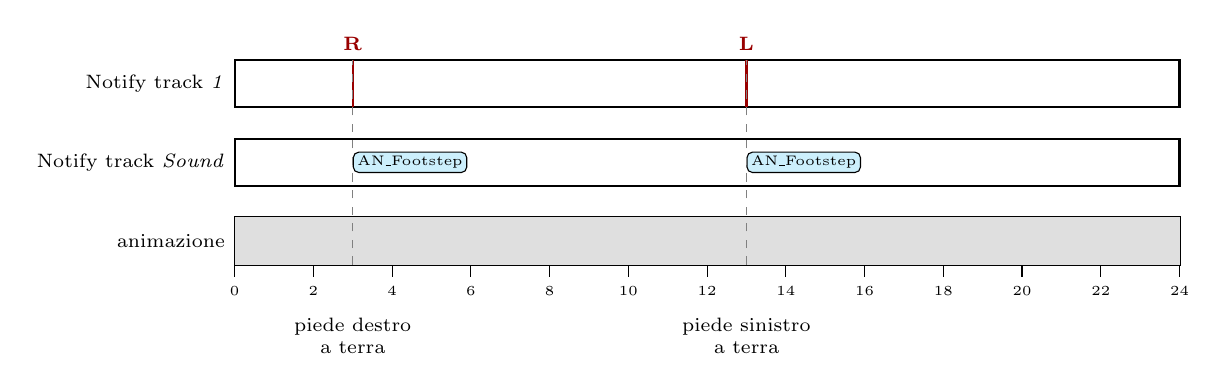
\begin{tikzpicture}[font=\footnotesize, x=0.5cm]
  \draw[thick] (0,0) rectangle (24,0.6);
  \node[left, font=\scriptsize] at (0,0.3) {Notify track \emph{1}};
  \draw[thick] (0,-1.0) rectangle (24,-0.4);
  \node[left, font=\scriptsize] at (0,-0.7) {Notify track \emph{Sound}};
  \draw[thick] (0,-2.0) rectangle (24,-1.4);
  \node[left, font=\scriptsize] at (0,-1.7) {animazione};
  \foreach \f in {0,2,...,24} {\draw (\f,-2.0) -- (\f,-2.15);
    \node[below, font=\tiny] at (\f,-2.15) {\f};}
  \fill[gray!25] (0,-2.0) rectangle (24,-1.4);
  \foreach \f/\n in {3/R, 13/L} {
    \draw[red!60!black, thick] (\f,0) -- (\f,0.6);
    \node[red!60!black, font=\scriptsize\bfseries, above] at (\f,0.6) {\n};
    \node[draw, fill=cyan!20, rounded corners=2pt, font=\tiny, inner sep=1.5pt, anchor=west]
      at (\f,-0.7) {AN\_Footstep};
    \draw[dashed, gray] (\f,-2.0) -- (\f,0.6);
  }
  \node[font=\scriptsize, align=center] at (3,-2.9) {piede destro\\a terra};
  \node[font=\scriptsize, align=center] at (13,-2.9) {piede sinistro\\a terra};
\end{tikzpicture}
\caption{La linea del tempo della corsa del bot (e delle due corse inclinate). Sulla
traccia \emph{1} i Sync Marker R e L ai frame 3 e 13; su una nuova traccia \emph{Sound}
l'AN\_Footstep negli stessi due punti. La lunghezza della linea del tempo è indicativa:
il numero totale di frame dell'animazione non si sente nella trascrizione. Schema
ricostruito.}
\label{ue10:fig:track}
\end{figure}

\paragraph{Approfondimento: Sync Marker, Blend Space e Notify doppi.} I Sync Marker non
sono legati alle ossa, come la trascrizione può far pensare, ma alla linea del tempo:
sono etichette con un nome (qui R e L) che segnano le fasi del passo. Servono quando
Unreal deve mescolare animazioni di durata diversa, nei Blend Space o con i
\emph{Sync Group}: invece di allinearle per tempo normalizzato, le allinea per marker, in
modo che i piedi tocchino terra insieme in tutte le animazioni mescolate. Funziona solo se
tutte le animazioni hanno gli stessi marker, con gli stessi nomi: è il motivo pratico per
cui il docente li aggiunge a tutte e tre le corse. I Notify, invece, pongono una domanda
diversa: in un Blend Space che sta mescolando tre animazioni, \emph{di quale} animazione
devono scattare i Notify? Nei Details del Blend Space, nella sezione \emph{Animation
Notifies}, l'opzione \emph{Notify Trigger Mode} decide: \emph{All Animations} (tutte quelle
che hanno un peso, con il rischio di sentire due o tre passi sovrapposti),
\emph{Highest Weighted Animation} (solo quella che pesa di più, la scelta più sicura per i
passi) o \emph{None}. Da notare infine che, nella lezione, la camminata a 250 non riceve
il Notify: a velocità intermedie i passi si sentono solo se il campione dominante è una
delle corse; per un risultato completo va aggiunto anche alla camminata, ai suoi frame di
appoggio. L'editor delle animazioni offre anche un Notify già pronto,
\emph{Play Sound}, che suona un suono senza Blueprint (il suo limite è che non sa
distinguere le superfici), e i \emph{Notify State}, che hanno un inizio e una fine invece
di un istante.

% ---------------------------------------------------------------------
\section{I Physical Material e le pedane}
\label{ue10:sec:physmat}

``Adesso, se noi andiamo in play, andiamo a vedere. Guardate un po'.'' A ogni passo
compare il trace che identifica il terreno, ``in questo caso il terreno di default''. ``Ma
come facciamo a dire, guarda, questo è un terreno diverso da quello normale? Dobbiamo
usare i Physics Material.''

\paragraph{Creare i Physical Material.} Una cartella \textbf{PhysicsMaterial} (``eccola
qua''); dentro, tasto destro, \textbf{Physics} $\rightarrow$ \textbf{Physical Material}. Se
ne creano due: \textbf{PM\_Rock} e \textbf{PM\_Water}. Poi, ``una cosa molto semplice,
ragazzi'': doppio clic su ciascuno; c'è la proprietà \textbf{Surface Type}, che di default
vale \emph{Default}: per PM\_Water si sceglie \textbf{Water}, per PM\_Rock \textbf{Rock}.
I nomi sono quelli scritti nelle Project Settings (figura~\ref{ue10:fig:catena}).

\paragraph{Le pedane.} ``L'unica cosa che ci manca è prendere una qualsiasi superficie.'' Un
blocco del livello, clonato (\textbf{Alt} più trascinamento, o duplicato) e schiacciato:
``fate un pianerottolino piccoletto'', due pedane. ``Adesso non abbiamo i materiali, ad
esempio, dell'acqua e della terra, ma ne mettiamo due a caso'': un materiale \emph{solid
blu} per l'acqua, \emph{Boulder} per la roccia; sono solo un segnale visivo. Poi:
selezionata la Static Mesh, ``andiamo giù, giù, giù, fino a trovare il \textbf{Phys
Material Override}'', e lì \textbf{PM\_Water} per l'acqua, \textbf{PM\_Rock} per la
roccia. ``Adesso, se noi andiamo sopra con il character, sentiamo che'' sulla roccia il
passo cambia. ``Eccolo qua.''

\begin{figure}[htbp]
\centering
\begin{tikzpicture}[font=\footnotesize,
  ue10box/.style={draw, thick, rounded corners=4pt, align=center, fill=gray!8,
                 minimum height=1.1cm, text width=2.5cm},
  ue10arr/.style={-{Stealth[length=2.5mm]}, thick}]
  \node[ue10box, fill=blue!8] (ps) at (0,0) {\textbf{Project Settings}\\{\scriptsize
    Engine, Physics, Physical Surface: Rock, Water}};
  \node[ue10box, fill=orange!12] (pm) at (4.3,0) {\textbf{PM\_Rock}, \textbf{PM\_Water}\\
    {\scriptsize Physical Material, Surface Type}};
  \node[ue10box, fill=green!10] (sm) at (8.6,0) {\textbf{Pedana}\\{\scriptsize Static
    Mesh, Phys Material Override}};
  \node[ue10box, fill=yellow!15] (tr) at (12.9,0) {\textbf{AN\_Footstep}\\{\scriptsize
    trace, Hit Result, Get Surface Type, Switch}};
  \node[ue10box, fill=violet!12] (cue) at (12.9,-2.4) {\textbf{Sound Cue}\\{\scriptsize
    Footstep, Rock, Water}};
  \node[ue10box, fill=red!10] (an) at (8.6,-2.4) {\textbf{Animazioni di corsa}\\
    {\scriptsize Notify ai frame 3 e 13}};
  \draw[ue10arr] (ps) -- node[above, font=\scriptsize]{nomi} (pm);
  \draw[ue10arr] (pm) -- node[above, font=\scriptsize]{assegnato} (sm);
  \draw[ue10arr] (sm) -- node[above, font=\scriptsize]{colpita} (tr);
  \draw[ue10arr] (tr) -- node[right, font=\scriptsize]{sceglie} (cue);
  \draw[ue10arr] (an.north east) -- node[below right, font=\scriptsize, pos=0.4]{fa
    scattare} (tr.south west);
\end{tikzpicture}
\caption{La catena completa dei passi. I nomi delle superfici nascono nelle Project
Settings, vengono assegnati ai Physical Material, che a loro volta si assegnano alle
superfici del livello; a ogni passo, il Notify inserito nell'animazione lancia il trace,
legge la superficie colpita e sceglie il Sound Cue. Schema ricostruito.}
\label{ue10:fig:catena}
\end{figure}

\paragraph{La spiegazione ripetuta.} A uno studente che chiede dove trovare ``i cosini''
(i PM): ``quelli li crei, praticamente. Lo fai con tasto destro, Physics, Physical
Material, e lo crei. Lo chiami PM\_Rock, come vuoi, PM\_Rock e PM\_Water. Ci clicchi su
ognuno di essi e gli cambi il Surface Type: lo metti Rock per il rock e Water per il
water. Poi, fatto questo, prendi un qualsiasi asset (vabbè, anche un blocco va
benissimo): devi andare su Phys Material Override e gli metti il Physical Material.''
``Basta che fai due pedanine'': ``qualsiasi superficie che tu vuoi prendere, ci puoi
camminare sopra''; ``la scali, fai quello che vuoi, fondamentalmente''.

\paragraph{Approfondimento: dove si assegna un Physical Material.} Il \emph{Phys Material
Override} usato a lezione vale per tutto il componente: comodo per una pedana, poco
pratico per un terreno che cambia da un punto all'altro. Unreal offre altri due posti. Il
primo è il \textbf{materiale}: nei Details di un Material (o di un Material Instance) c'è
la proprietà \emph{Phys Material}; tutte le mesh che usano quel materiale ``diventano''
roccia o acqua, senza toccare il livello, ed è la soluzione abituale nei progetti veri.
Il secondo è il \textbf{Landscape}: ogni layer dipinto può avere il suo Physical Material,
e il trace legge quello del layer dominante nel punto colpito. In più, il Physical
Material non serve solo ai suoni: contiene l'attrito (\emph{Friction}), il rimbalzo
(\emph{Restitution}) e la densità usati dalla simulazione fisica, ed è la base per gli
effetti d'impatto dei proiettili (scintille sul metallo, polvere sulla pietra), con la
stessa tecnica del Get Surface Type e dello Switch.

% ---------------------------------------------------------------------
\section{Gli ultimi problemi e la chiusura}
\label{ue10:sec:chiusura}

\paragraph{Gli ultimi problemi.} ``Un attimo: è successo un casino? Gli altri? Qualche
problema? Funziona?''
\begin{itemize}
  \item Uno studente si è perso il primo pezzo del grafo dell'AN\_Footstep e non sa da
        dove vengano Mesh Comp, Animation ed Event Reference: sono gli ingressi di
        Received\_Notify, la funzione sovrascritta con \emph{Override}. Poi, di nuovo, la
        catena: ``Get Owner, Get Actor Location, Get Actor Up Vector, e poi sottrai,
        per far sì che'' End sia sotto lo Start, ``che è il Get Actor Location''.
  \item Lo stesso studente ha messo le pedane, ma il personaggio non fa nessun rumore,
        nemmeno sul pavimento normale. I suoni nell'Anim Notify ci sono (``Rock1, Water
        Cue, Footstep Cue: va benissimo''); l'errore è nel vettore: il Get Actor Up Vector
        era collegato al pin sbagliato del Multiply. ``Mettilo sopra; stacca quello
        sotto; tasto destro su quello là, to float, 250.'' Con il Draw Debug Type a For
        Duration e una ricompilazione, il passo si sente.
  \item Le pedane, però, non fanno il suono della roccia: ``fammi vedere se hai messo la
        cosa'', e infatti il Phys Material Override non c'era. Lo studente non riesce a
        scendere nei Details fino alla voce: il pannello era filtrato su una categoria
        (\emph{Generale}); cliccando su \emph{Tutto} e aprendo la parte avanzata della
        sezione \emph{Physics} (``vai su tutto, clicca su tutto; giù, eccolo là''), si
        trova \emph{Phys Material Override}. ``A posto, perfetto.''
  \item ``A me non compaiono le linee'': ``basta che fai Draw Debug Type e la metti For
        Duration'', sul Line Trace By Channel. ``Quello è solo una cosa di debug,
        tranquilli.''
\end{itemize}

\paragraph{L'inclinazione rimandata.} ``Io ho sempre quella cosa dell'inclinazione della
testa'': è la studentessa del Lean che non inclina. ``Possiamo farlo la prossima volta?''
``Sì, facciamo la prossima volta. Tanto la prossima volta facciamo interazioni, e allora
ricordamelo tu, eh?'' ``Così fixiamo tutto''; ``lo guardo poi in futuro, lo guardo poi in
post anche''.

\paragraph{Il calendario.} ``Io vi ringrazio per l'attenzione, grazie'' anche a chi segue
in differita. ``Ci vediamo giovedì per la prossima lezione, che faremo in questo caso i
menu: andiamo a fare un po' di UI.'' (Il docente, poco prima, aveva parlato di
``interazioni'': dalla trascrizione non si capisce se la lezione di giovedì conterrà
entrambe le cose.) Uno studente pensava che oggi fosse giovedì; il calendario: ``abbiamo
questo martedì, giovedì e, se non sbaglio, il 30, che è martedì prossimo: è l'ultima con
me. Poi ci avete Davide.'' ``Va bene, ragazzi. Allora ci vediamo. Buona cena. Buona
serata.''

\begin{table}[htbp]
\centering
\small
\begin{tabular}{@{}p{5.4cm}p{8.6cm}@{}}
\toprule
\textbf{Sintomo} & \textbf{Causa e rimedio} \\
\midrule
Il personaggio non si muove, errori su IA\_Run & IA\_Move cancellata e sostituita da
IA\_Run: duplicare IA\_Look (Vector 2D), rinominarla IA\_Move, rimetterla in IMC\_Default
e nell'evento \\
L'evento del movimento non mostra il vettore & salvare l'Input Action; poi Split Struct
Pin sull'Action Value \\
Dopo una compilazione ``sparisce tutto'' & il Blueprint non compila: leggere i Compiler
Results \\
Camera storta, movimento strano & Spring Arm attaccato alla freccia o spostato dal pivot:
riattaccarlo, location a zero, usare Target Arm Length, Socket Offset, Target Offset \\
La camera non segue il mouse & Use Pawn Control Rotation sullo Spring Arm \\
La torretta ignora il nuovo personaggio & manca il tag Player; controllare le risposte
ai trace e alle collisioni \\
Il Montage non si vede & manca lo Slot DefaultSlot nell'AnimGraph \\
Durante il Montage il corpo gira & il DefaultSlot prende tutte le ossa: serve uno slot
per la parte alta (Layered blend per bone) \\
Errori nell'Event Graph incollato & variabili del vecchio ABP: ricrearle con Create
variable, rifare le referenze nell'Initialize \\
\emph{Idle to Walk will never be taken} & la regola della transizione non è ancora
scritta \\
Lo stato non mostra l'anteprima del Blend Space & lo stato non è mai raggiunto
(transizione o dati mancanti) \\
Il personaggio levita & Mesh a Z = $-90$ \\
Il personaggio si muove in T-pose & State Machine non collegata all'Output Pose, o
Mesh senza Anim Class \\
Errori su Jump e Fall & regole vuote: Automatic Rule Based on Sequence Player in State, e
la regola Fall $\rightarrow$ Land Run \\
GroundSpeed sempre zero & due variabili Character Movement (una mai valorizzata), o
Update non collegato al Validated Get \\
Il Lean non inclina & segno e scala del Delta Rotator, opzioni di rotazione; rimandato
alla lezione successiva \\
La camera inclinata di lato & ruotata sulla X (Roll) invece che sulla Y (Pitch) \\
AN\_Footstep non compare in Add Notify & la classe ha un altro nome: cercarla con quello
\\
Nessun suono di passi & Up Vector sul pin sbagliato del Multiply; Notify non inserito
nelle animazioni \\
Le pedane suonano come il pavimento & manca il Phys Material Override, o il Surface Type
del Physical Material \\
Phys Material Override introvabile & filtro dei Details su Generale: scegliere Tutto e
aprire le opzioni avanzate \\
Le linee del trace non si vedono & Draw Debug Type a For Duration \\
\bottomrule
\end{tabular}
\caption{I problemi incontrati durante la lezione, con la causa e il rimedio.}
\label{ue10:tab:errori}
\end{table}

\begin{table}[htbp]
\centering
\small
\begin{tabular}{@{}p{4.8cm}p{9.2cm}@{}}
\toprule
\textbf{Nodo, asset o impostazione} & \textbf{Che cosa fa} \\
\midrule
Input Action, Value Type Vector 2D & azione con un valore a due assi (movimento,
sguardo) \\
Add Movement Input & muove il Pawn lungo una direzione, con una scala \\
Tags (Actor) & etichette con cui altri Blueprint riconoscono l'actor \\
Try Get Pawn Owner / Cast To & il Pawn che possiede l'animazione; la sua classe precisa \\
Promote to Variable & salva un'uscita in una nuova variabile \\
Convert to Validated Get & Get con controllo di validità (Is Valid / Is Not Valid) \\
Create variable (tasto destro) & crea la variabile mancante di un nodo incollato \\
Comment (tasto C) / Reroute Node (doppio clic sul filo) & riquadro con titolo; punto di
piegatura di un filo \\
Blend Space 2D: Lean e GroundSpeed & mescola le corse inclinate e la camminata \\
Get Owning Actor / Get Actor Rotation & l'actor proprietario; la sua rotazione \\
Delta Rotator & la differenza normalizzata fra due rotazioni \\
FInterp To / RInterp To & un passo d'interpolazione fra float; fra rotator \\
Get World Delta Seconds & il tempo dell'ultimo frame \\
State Machine, Can Enter Transition & stati e regole booleane di passaggio \\
Automatic Rule Based on Sequence Player in State & la transizione scatta a fine
animazione \\
AND Boolean / NOT Boolean & congiunzione; negazione \\
Get Last Input Vector & l'ultimo input di movimento del Pawn (lunghezza 0--1) \\
Vector Length & la lunghezza di un vettore \\
Print String & scrive un valore a schermo, per il debug \\
World Settings: Default Pawn Class & il personaggio del giocatore nel livello \\
Anim Notify (classe), Received\_Notify & evento in un istante dell'animazione; la funzione
che lo riceve \\
Get Owner / Get Actor Location / Get Actor Up Vector & proprietario; posizione; vettore
verso l'alto \\
Line Trace By Channel, Draw Debug Type & trace lungo un segmento; disegno di debug \\
Break Hit Result: Impact Point & il punto esatto dell'impatto \\
Get Surface Type & il tipo di superficie colpita (dal Physical Material) \\
Physical Surface (Project Settings) & i nomi dei tipi di superficie \\
Switch on EPhysicalSurface & un'uscita per ogni tipo di superficie \\
Play Sound at Location & suona un suono in un punto \\
Sound Wave / Sound Cue & file audio; grafo che combina e modula i suoni \\
Create Single Cue & crea un Cue dai Sound Wave selezionati (con Random) \\
Random / Modulator & sceglie un ingresso a caso; varia pitch e volume \\
Add Sync Marker & marcatore con nome sulla linea del tempo (R, L) \\
Insert Notify Track / Add Notify & nuova traccia di Notify; inserisce un Notify \\
Physical Material: Surface Type & il tipo di superficie dell'asset \\
Phys Material Override & assegna un Physical Material a un componente \\
\bottomrule
\end{tabular}
\caption{I nodi, gli asset e le impostazioni della decima lezione.}
\label{ue10:tab:nodi}
\end{table}

% ---------------------------------------------------------------------
\section*{Punti chiave del capitolo}
\addcontentsline{toc}{section}{Punti chiave del capitolo}

\begin{itemize}
  \item Un'\textbf{Input Action} cancellata rompe il personaggio in modo silenzioso: si
        ricrea duplicando un'azione dello stesso tipo (\textbf{IA\_Look}, Vector 2D, per
        \textbf{IA\_Move}), la si rimette nell'\textbf{IMC} e nell'evento. Lo
        \textbf{Spring Arm} non si sposta dal pivot: si regolano Target Arm Length,
        Socket Offset e Target Offset.
  \item Quando si cambia personaggio, tutto ciò che riconosceva il vecchio va
        ricontrollato: \textbf{tag} (Player per la torretta), \textbf{cast} a classi
        precise, \textbf{collisioni} e risposte ai trace.
  \item Un Animation Blueprint si può costruire \textbf{copiando} l'Update di un altro, ma
        l'\textbf{Initialize} si rifà: Try Get Pawn Owner, Cast To, referenze promosse a
        variabile, ``un gancio'' fra animazione e personaggio. Le variabili mancanti si
        ricreano con \textbf{Create variable}; il \textbf{Validated Get} protegge l'Update.
        Attenzione alle variabili doppie (Character Movement 0).
  \item Ordine nel grafo: \textbf{commenti} con il tasto C, \textbf{Reroute} con un doppio
        clic sul filo.
  \item Il \textbf{Blend Space 2D} del bot ha il \textbf{Lean} in orizzontale ($-10$,
        10) e la \textbf{GroundSpeed} in verticale (0--500, la Max Walk Speed): corsa e
        corse inclinate a 500, camminata a 250, nessun Idle.
  \item Il \textbf{Lean} si calcola a ogni frame: rotazione attuale, \textbf{Delta
        Rotator} con quella precedente, lo \textbf{Yaw}, \textbf{FInterp To} verso quel
        valore (Interp Speed 1--5, Get World Delta Seconds), poi la rotazione attuale
        diventa la precedente. Segno e scala vanno verificati.
  \item La \textbf{State Machine} ha sette stati: Idle e Walk (GroundSpeed $>$ 0, $\le$
        0), Jump Idle e Jump Run (IsFalling AND la velocità), Fall (automatica dopo i
        salti), Land Idle e Land Run (NOT IsFalling AND [NOT] \textbf{ReceiveInput}),
        ritorni automatici. ReceiveInput viene da \textbf{Get Last Input Vector}: la
        lunghezza maggiore di zero dice che il giocatore sta premendo.
  \item Per giocare con il bot: Spring Arm e Camera a zero, Target Offset, \textbf{Default
        Pawn Class} nelle World Settings, i grafi di input copiati dal vecchio
        personaggio, Use Pawn Control Rotation, Mesh a $-90$.
  \item I passi: un \textbf{Anim Notify} (AN\_Footstep, \textbf{Received\_Notify}) lancia
        un \textbf{Line Trace By Channel} di 250 centimetri verso il basso; dal Hit Result,
        \textbf{Get Surface Type} e \textbf{Switch on EPhysicalSurface} scelgono il
        \textbf{Play Sound at Location} sull'\textbf{Impact Point}.
  \item I tipi di superficie si definiscono nelle \textbf{Project Settings} (Physics,
        Physical Surface: Rock, Water); i \textbf{Physical Material} (PM\_Rock, PM\_Water)
        li assegnano con il Surface Type; il \textbf{Phys Material Override} li applica
        alle mesh del livello.
  \item I \textbf{Sound Cue} variano i passi: \textbf{Random} fra più Sound Wave
        (\emph{Create Single Cue}) e \textbf{Modulator} sul pitch (passo 0,95--1,3, roccia
        2--2,2, acqua 1,3--1,5).
  \item Nelle animazioni di corsa: \textbf{Sync Marker} R e L e una \textbf{Notify Track}
        \emph{Sound} con l'AN\_Footstep ai frame di appoggio (3 e 13), in tutte e tre le
        animazioni.
\end{itemize}
